\documentclass[]{phdthesis}
\addbibresource{../../references/thesis_n.bib}

\degree{Doctor of Philosophy}
\university{University College London}
\title{Computational design and\\[0.2em]characterisation of synthetic\\[0.2em] genetic switches}
\author{Miriam Leon}
\primarysupervisor{Dr. Chris P Barnes}
\secondarysupervisor{Prof. Geraint MH Thomas}

%%  Abbreviations entries  -----------------%%
%\acrlong{ } whole phrase, \acrshort{ } acronym, \acrfull{ } both
\makeglossaries
\newacronym{ode}{ODE}{Ordinary differential equation}
\newacronym{abc}{ABC}{Approximate Bayesian Computation}
\newacronym{smc}{SMC}{Sequential Monte Carlo}
\newacronym{mcmc}{MCMC}{Markov Chain Monte Carlo}
\newacronym{sde}{SDE}{Stochastic differential equation}
\newacronym{mjp}{MJP}{Markov jump process}
\newacronym{gpu}{GPU}{Graphical Processing Units}

\newacronym{pdf}{PDF}{probability density function}
\newacronym{cuda}{CUDA}{Compute Unified Device Architecture}
\newacronym{qssa}{QSSA}{quasi-steady state approximation}
\newacronym{pca}{PCA}{Principal component analysis}

\newacronym{ks}{KS}{Kolmogorov-Smirnov}

\newacronym{cs-ma}{CS-MA}{Mass action classic switch}
\newacronym{dp-ma}{DP-MA}{Mass action double positive switch}
\newacronym{sp-ma}{SP-MA}{Mass action single positive switch}
\newacronym{cs-lu}{CS-LU}{Lu classic switch}
\newacronym{sp-lu}{SP-LU}{Lu single positive switch}
\newacronym{dp-lu}{DP-LU}{Lu double positive switch}
\newacronym{kde}{KDE}{Kernel density estimation}
%\newacronym{1d}{1D}{one dimensional}
%\newacronym{2d}{2D}{two dimensional}
\newacronym{pcr}{PCR}{Polymerase Chain Reaction}
\newacronym{atc}{ATc}{anhydrotetracycline}
\newacronym{iptg}{IPTG}{Isopropyl-beta-D-thiogalactopyranoside}
\newacronym{dna}{DNA}{Deoxyribonucleic acid}
\newacronym{lb}{LB}{Lysogeny broth}
\newacronym{dntp}{dNTPs}{Deoxynucleotide}
\newacronym{bsa}{BSA}{Bovine Serum Albumin}
\newacronym{gfp}{GFP}{green fluorescent protein}

%%---------------------------------------------------%%
\begin{document}
% front matter
\maketitle


\begin{abstract}
blabla
\end{abstract}

\tableofcontents*
\listoffigures
\listoftables
\glossarystyle{list}

\printglossary[type=\acronymtype, title=Abbreviations, toctitle=List of abbreviations]

%\printglossary[type=\acronymtype, title=Abbreviations, toctitle=Abbreviations]

\begin{acknowledgements}
blabla
\end{acknowledgements}

%% --------------------------------------------------------------
%% CHAPTERS
%% --------------------------------------------------------------

%% Introduction -------------------------------------%%
\mainmatter*
\chapter{Introduction}
\label{ch:Intro}


\section{Introduction to synthetic biology}

Synthetic biology aims at the rational design and construction of biological parts, devices, and systems in order to engineer organisms to perform new tasks~\autocite{Lu:2009ez, Andrianantoandro:2006bia}. A part is a basic unit, like a promoter or a ribosome binding site that when combined with other parts will make a functional unit, a device~\autocite{Heinemann:2006ht}. A device processes inputs, performs functions and produces outputs~\autocite{Andrianantoandro:2006bia}. A system comprises of a collection of devices.     

Emphasis is put on the use of engineering principles such as modularity, standardisation, use of predictive models and the separation of design and construction~\autocite{Agapakis:2009bt, Heinemann:2006ht}. A hierarchy similar to computer science is used, with cells, pathways and biochemical reactions acting as computers, modules and gates respectively~\autocite{Andrianantoandro:2006bia}. 
       
Numerous applications of synthetic biology have emerged, from altering existing metabolisms to producing synthetic drugs ~\autocite{Holtz:2010bm} or creating new synthetic life forms ~\autocite{Agapakis:2009bt}. Despite the successes there is still a lack of predictive power due to the stochasticity and lack of complete knowledge of the cellular environment ~\autocite{Andrianantoandro:2006bia}.

Synthetic biology is now entering an age where simple synthetic circuits have been built, such as toggle switches \autocite{Gardner:2000vha, Kramer:2004kq, Isaacs:2003hta, Ham:2008hh, Deans:2007cy, Friedland:2009ce}, oscillators~\autocite{Stricker:2008jqa, Fung:2005jd, Tigges:2009jx} and pulse generators~\autocite{Basu:2004gn}, but larger circuits have proven more difficult \autocite{XXX}. The leap from building low-level circuits to assembling them into complex networks has yet to be made successfully~\autocite{Lu:2009ez}, and predictable circuit behaviour remains challenging~\autocite{XXX}. Efforts to do so are plagued by intra-circuit crosstalk and incompatibility, as well as cellular noise, which can render synthetic networks non-functional \textit{in vivo} \autocite{XXX}. 


\section{Quantitative modelling in synthetic biology}

Importance of quantitative understanding of systems

mathematical modelling can aid the advancement of the field of synthetic biology

Synthetic biology draws from the multidisciplinary work of biologists, mathematicians, computer scientists, physicists, to name a few examples. The work from a lot of different fields comes together to attempt to engineer biology. The randomness of the biological environment, the plethora of unknowns in the engineered system as well as its surrounding environment and their interaction therein makes this task extremely challenging. The field has made great advancements in recent years(XXX), and mathematical modelling has played an integral part in that(XXX). 


Statistical tools are being developed that can handle the complexity of synthetic biological models(XXX).

The field of systems biology has aided in the advancement of the field(XXX). It aims to understand of the underlying principles that govern system dynamics. It aims to uncover the signal within the noise, or to understand the significance of noise itself in the function of the system(XXX)


Here I use quantitative modelling to understand a synthetic system. I look at the problem from two different perspectives, design and inference. I aim to improve on the design of a synthetic biological system and understand the principles dictating the new designs. I also aim to quantitatively study the current system and infer the underlying principles that govern its behaviour.  


\section{Thesis Outline}

This thesis will focus on the biochemical modelling of the genetic toggle switch. The thesis is organised as follows:

\vskip 0.1in
\noindent \textbf{Chapter 2} provides an introduction to biochemical modelling. It contains an overview of the mathematical methods that formed the basis of the methods used throughout this thesis. It also contains a literature review on the current understanding on the dynamics of the genetic toggle switch. I provide material that is necessary for the understanding of the rest of this thesis. 
\vskip 0.1in
\noindent In \textbf{Chapter 3} I explore the effect that adding feedback loops has on the stability and parametric robustness of the toggle switch. I develop more realistic biochemical models of the genetic toggle switch and study their ability to behave like a switch.  

\vskip 0.1in
\noindent In \textbf{Chapter 4} I develop a parameter estimation algorithm for multistable switches, called StabilityFinder. I benchmark this algorithm using a toggle switch model with known results. I then apply it to extensions of the simplified toggle switch as well as the more realistic models of the toggle switch developed in Chapter 4 in order to study the design principles that make a multistable switch. Finally I develop an algorithm for estimating the robustness of a system using the results from StabilityFinder and use it to study the effect of feedback loops on the robustness of the switch.  

\vskip 0.1in
\noindent In \textbf{Chapter 5} I develop an algorithm based on bayesian statistics for parameter estimation for biochemical modelling of flow cytometry data, called ABC-Flow. I also characterise the genetic toggle switch experimentally and provide an overview of the methods used. Finally I apply ABC-FLow to the experimental data collected and infer the parameters that give rise to the data.
\vskip 0.1in
\noindent In \textbf{Chapter 6} contains a detailed experimental plan to be carried out as a next step to this work. I outline the steps needed to design and construct genetic toggle switches with added autoregulating feedback loops experimentally. 
\vskip 0.1in
\noindent \textbf{Chapter 7} concludes this thesis with an overview of the work presented here and a discussion of future directions. 
\vskip 0.1in
\noindent Work carried out throughout my candidature has been published in the following articles:

\begin{enumerate}
	\item Leon, M., Woods, M., Fedorec, J. A., \& Barnes, C. P. (2016). ‘A computational method for the investigation of multistable systems and its application to genetic switches’. [Submitted].
	\item Woods, M. L., Leon, M., Perez-Carrasco, R., \& Barnes, C. P. (2016). ‘A Statistical Approach Reveals Designs for the Most Robust Stochastic Gene Oscillators.’ ACS Synthetic Biology 5(6), 459–470.
	
\end{enumerate}

%% Background -------------------------------------%%
\mainmatter*
\chapter{Background}
\label{ch:backg}


%\section{System design in synthetic biology}

\section{Current understanding of the genetic toggle switch}

One of the first successfully constructed synthetic devices is the genetic toggle switch. A toggle switch consists of a set of transcription factors that mutually repress each other~\autocite{Gardner:2000vha}. Genetic switches play a major role in binary cell fate decisions like stem cell differentiation, as they are capable of exhibiting bistable behaviour. Bistability of a system is defined by the existence of two distinct phenotypic states but no intermediate state. Bistability is a property that is important in nature and a valuable resource to exploit in synthetic biology. It allows cells to alter their response to environmental cues and increases the overall population fitness by 'hedge-betting' the response of the population \autocite{Veening:2008da}. 

\subsection{The genetic toggle switch in natural systems}
In developmental processes, bistability ensures that the differentiating cell will follow one pathway, or the other, with no possible intermediate phenotypes. This is vital for the correct development of a cell in a specific pathway. One example is the trophectoderm differentiation pathway, in which a mutually inhibitory toggle switch exists between Oct3/4 and Cdx2. This determines whether an embryonic stem cell will differentiate into a trophectoderm cell, if Cdx2 dominates the system, or an inner cell mass cell if Oct3/4 dominates~\autocite{Niwa:2005fz}. Bistability is critical in this system as a cell must differentiate into either a trophectoderm cell or an inner cell mass cell and there should not be any intermediate signals. 

In the case of the GATA1 and PU.1 toggle switch, the transcription factor pair controls the fate of the common myeloid progenitors, and the two possible differentiation paths are erythroid and myeloid blood cells~\autocite{Liew:2006cd}. The double-negative feedback loop created by the mutually repressive pair of transcription factors sustains the system in balance until an external stimulus causes one of the two transcription factors to increase in concentration. The increased concentration of one transcription factor causes the increased repression of the production of the antagonistic transcription factor, tipping the balance towards the dominance of the first transcription factor. The double negative feedback loop reinforces this dynamic and the system remains in the same state until an external stimulus disturbs it~\autocite{FerrellJr:2002fh}.

\subsection{Uses in synthetic biology}
Despite their simplicity, toggle switches can be powerful building blocks with which to create complex responses in a synthetic network~\autocite{Lu:2009ez}. They can be used in isolation and have the potential to be used tandem to create complex networks and signalling cascades~\autocite{Lu:2009ez}. The toggle switch has been used for the regulation of mammalian gene expression~\autocite{Deans:2007cy, Kramer:2004kq}. Other synthetic applications of the toggle switch include the construction of a synthetic genetic clock~\autocite{Atkinson:2003tu}, of a predictable genetic timer~\autocite{Ellis:2009hka}, and the formation of biofilms in response to engineered stimuli~\autocite{Kobayashi:2004cv}. 

These applications are modifications of the classical toggle switch~\autocite{Gardner:2000vha}, but an application made of a cascade or collection of the switch would be more challenging. This would make more complex applications possible and could be used to solve real-life problems. For example, an analog-to-digital converter to translate external stimuli like the concentration of an inducer into an internal digital response, or programmable bacteria to move from point to point up different chemical gradients~\autocite{Lu:2009ez}. For a review on current circuits see~\autocite{Khalil:2010hm} and for possible future applications see~\autocite{Lu:2009ez}. This leap will be difficult to achieve before first being able to build robust and well characterised individual switches.

\subsection{Modelling the genetic toggle switch} 

%Deterministic modelling utilises ordinary differential equations (ODE) and models the concentrations of the species (proteins or other molecules) by time-dependent variables~\autocite{deJong:2002ft}. When modelling deterministically the model is viewed as a system whose behaviour is entirely predictable, given sufficient knowledge. In stochastic modelling, species are measured in discrete amounts rather than concentrations and a joint probability distribution is used to express the probability that at time \textit{t} the cell contains a number of molecules of each species~\autocite{deJong:2002ft,Wilkinson:2006td}. It takes uncertainty into account and is thus often more appropriate for modelling cellular systems, although more computationally expensive. In stochastic systems the Gillespie algorithm is widely used to simulate the time-evolution of the state of the system~\autocite{Warren:2005kea}.

The toggle switch motif has been studied extensively and there are numerous studies based on a number of different methods of modelling and analysis of the dynamics, including both deterministic and stochastic approaches. The conclusions drawn about the stability and robustness of the toggle switch vary between the different modelling approaches. Numerous studies have concluded that cooperativity is a necessary condition for bistability to arise~\autocite{Gardner:2000vha, Walczak:2005ds, Warren:2004baa, Warren:2005kea, Cherry:2000wi}. However, ~\textcite{Lipshtat:2006wb} found that stochastic effects can give rise to bistability even without cooperativity in three kinds of switch; the exclusive switch, in which there can only be one repressor bound at any one time, a switch in which there is degradation of bound repressors, and the switch in which free repressor proteins can form a complex, which renders them inactive as transcription factors~\autocite{Lipshtat:2006wb}. 

In another study, \textcite{Ma:2012dt} found that the stochastic fluctuations in a system involving such a small number of molecules, like the toggle switch, uncovers effects that cannot be predicted by the fully deterministic case~\autocite{Ma:2012dt}. In their system, the toggle switch was found to be tristable, as small number effects render the third unstable steady state stable. \textcite{Biancalani:2015vya} identified multiplicative noise as the source of bistability in the stochastic case~\autocite{Biancalani:2015vya}.~\textcite{Warren:2005kea} concluded that the exclusive switch is always more robust than the general switch since the free energy barrier is higher~\autocite{Warren:2005kea}. A summary of the toggle switch models is shown in Table~\ref{tab:refs}. As is clear from above, there is yet to exist a consensus on the stability a switch is capable of, and the most appropriate method of modelling it. Different methods arrive at different conclusions, creating confusion on which behaviour to be expected by the experimentalist for even a simple system like the toggle switch, consisting of just two genes. The toggle switch cannot be used as a building block of larger, more complex systems until its behaviour can be predicted accurately. Until then, designing systems with predictable behaviour will be near impossible.


\begin{table}[t]
\centering

\caption{Summary of stabilities for the classical switch and the switch with double positive feedback found via different modelling approaches}
\label{tab:refs}
\rotatebox{90}{
\begin{tabular}{@{}llll@{}}
\toprule
\multicolumn{1}{c}{} & \multicolumn{2}{c}{Standard toggle switch} & \multicolumn{1}{c}{Double positive autoregulation} \\ \midrule
Stability & Deterministic & Stochastic & Deterministic \\
Monostable & \autocite{Loinger:2009vo} & \autocite{Loinger:2009vo} & \autocite{Guantes:2008gs} \\
\multirow{4}{*}{Bistable} & \autocite{Gardner:2000vha} & \autocite{Lu:2014kc}, & \multirow{4}{*}{\autocite{Guantes:2008gs}} \\
 & \autocite{Loinger:2009vo} & \autocite{Lipshtat:2006wb}, &  \\
 &  & \autocite{Biancalani:2015vya}, &  \\
 &  & \autocite{Loinger:2009vo} &  \\
\multirow{2}{*}{Tristable} & \multirow{2}{*}{} & \autocite{Loinger:2009vo}, & \autocite{Guantes:2008gs}, \\
 &  & \autocite{Ma:2012dt} & \autocite{Lu:2014kc} \\
Quadristable &  &  & \autocite{Guantes:2008gs} \\ \bottomrule
\end{tabular}
}
\end{table}

\clearpage


%\begin{table}[t]
%\centering
%\caption{Summary of stability for the CS switch found via different modelling approaches}
%\label{tab:refs}
%\begin{tabular}{@{}llll@{}}
%\toprule
%             & \multicolumn{2}{c}{CS}                                                                                                                                   & \multicolumn{1}{c}{DP}                      \\ \midrule
%Stability    & Deterministic                                      & Stochastic                                                                                          & Deterministic                               \\
%Monostable   & \autocite{Loinger:2009vo}                           & \autocite{Loinger:2009vo}                                                                            & \autocite{Guantes:2008gs}                     \\
%Bistable     & \autocite{Gardner:2000vha}, \autocite{Loinger:2009vo} & \cite{Lu:2014kc}, \autocite{Biancalani:2015vya}, \autocite{Lipshtat:2006wb}, \autocite{Loinger:2009vo} & \autocite{Guantes:2008gs}                     \\
%Tristable    &                                                    & \autocite{Loinger:2009vo}, \autocite{Ma:2012dt}                                                        & \autocite{Guantes:2008gs}, \autocite{Lu:2014kc} \\
%Quadristable &                                                    &                                                                                                     & \autocite{Guantes:2008gs}                     \\ \bottomrule
%\end{tabular}
%\end{table}

%\begin{table}[]
%\centering
%\caption{Summary of stability for the toggle switch found via different modelling approaches}
%\label{tab:refs}
%\rotatebox{90}{
%\begin{tabular}{@{}ccccccc@{}}
%\toprule
%                                        & \multicolumn{3}{c}{\textbf{Simple}}                                                                                                                                            & \multicolumn{3}{c}{\textbf{Double positive autoregulation}} \\ \midrule
%                                        & \textit{Stability}                             & \textit{Reference} & \textit{Notes}                                                                                           & \textit{Stability}  & \textit{Reference}  & \textit{Notes}  \\  \midrule
%\multirow{3}{*}{\textbf{Deterministic}} & Monostable                                     & \autocite{Loinger:2007vma}       & \begin{tabular}[c]{@{}c@{}}no cooperativity,\\ exclusive \& general\end{tabular}                         & Bistable            & \autocite{Guantes:2008gs}        &                 \\
%                                        & \multirow{2}{*}{Bistable}                      & \autocite{Gardner:2000vha}       & copperativity \textgreater 2,                                                                            & Tristable           & \autocite{Guantes:2008gs}        &                 \\
%                                        &                                                & \autocite{Loinger:2007vma}       & bound repressor degradation                                                                              & 4 steady steates    & \autocite{Guantes:2008gs}        &                 \\ \midrule
%\multirow{7}{*}{\textbf{Stochastic}}    & Monostable                                     & \autocite{Loinger:2007vma}       & \begin{tabular}[c]{@{}c@{}}no cooperativity, \\ weak repression\end{tabular}                             & Tristable           & \autocite{Lu:2014kc}             &                 \\
%                                        & \multirow{4}{*}{Bistable}                      & \autocite{Lu:2014kc}            &                                                                                                          &                     &                     &                 \\
%                                        &                                                & \autocite{Biancalani:2015vya}    & \begin{tabular}[c]{@{}c@{}}exclusive,\\ controlled by noise strength\end{tabular}                        &                     &                     &                 \\
%                                        &                                                & \autocite{Lipshtat:2006wb}      & no cooperativity                                                                                         &                     &                     &                 \\
%                                        &                                                & \autocite{Loinger:2007vma}       & \begin{tabular}[c]{@{}c@{}}no cooperativity,\\ exclusive \& \\ bound repression degradation\end{tabular} &                     &                     &                 \\
%                                        & \multicolumn{1}{l}{\multirow{2}{*}{Tristable}} & \autocite{Loinger:2007vma}       & \begin{tabular}[c]{@{}c@{}}no cooperativity,\\ strong repression\end{tabular}                            &                     &                     &                 \\
%                                        & \multicolumn{1}{l}{}                           & \autocite{Ma:2012dt}           &                                                                                                          &                     &                     &                 \\ \bottomrule 
%\end{tabular}
%}
%\end{table} 


\section{Methods in biochemical modelling}

Modelling attempts to describe the elements and dynamics of the biochemical system of interest. It is a tool used for integrating knowledge and experimental data as well as for predicting the behaviour of the system~\autocite{Wilkinson:2006td}. 


\subsection{Representation of transcription networks}
A transcription network can be represented in a number of ways. A network can be described by using a diagram supplemented by verbal explanations or by a set of differential equations. A diagram with a lengthy verbal explanation risks the not providing sufficient clarity whereas a set of differential equations cannot easily be separated from the underlying assumptions made on the kinetics of the network. A convenient way of describing sufficient information about a system while avoiding the addition of the particular interpretation of the underlying kinetics is the use of coupled chemical reactions~\autocite{Wilkinson:2006td}. 

\subsubsection{Coupled chemical reactions and the law of mass action}

Coupled chemical reactions are often used to describe transcription networks in systems biology. They have the advantage of describing a system concisely while they can be used subsequently for a variety of different simulation methods, each with their associated interpretation of chemical kinetics~\autocite{Wilkinson:2006td}. Coupled chemical reactions take the form


\begin{align}
	R_a + R_b \xrightarrow{k} P, \label{eq:example_eq}
\end{align}

\noindent where $R_a$ represents reactant A, $R_b$ reactant B and $P$ a product. Each reaction has an associated rate constant $k$. A biological transcription network can be represented using the above notations. Some common examples of coupled chemical reactions used in a biological network are given in Table~\ref{tab:chem_reac_ex}. A double headed arrow represents a reversible reaction. 


\begin{table}[tb]
\centering
\caption{Examples of common genetic coupled chemical reactions. $p$ stands for promoter, and $A$ represents a protein. $A_2$ is the dimer of protein $A$.  }
\label{tab:chem_reac_ex}
\begin{tabular}{@{}lll@{}}
\toprule
Event & Coupled chemical reaction & Rates\\ \midrule
Transcription & $p  \xrightarrow{k_1} p + RNA$ & $k_1[p]$\\
Dimerization & $2A \xrightleftharpoons[k_3]{k_2} A_2$&$ k_2[A][A]$, $ k_3[A_2]$\\
Promoter repression & $A_2 + p \xrightleftharpoons[k_5]{k_4} p\bullet A_2$& $ k_4[A_2][p]$, $ k_5[p\bullet A_2]$ \\
Activation & $A_2 + p \xrightarrow{k_6} p\bullet A_2 + RNA$ & $ k_6[A_2][p]$\\
Degradation & $A \xrightarrow{k_7}\varnothing $ &$k_7[A]$\\ \bottomrule
\end{tabular}
\end{table}

The law of mass action allows one to derive these reaction rates from the coupled chemical reactions. The assumption made in the law of mass action is that the system exists in a well-mixed solution and in dynamic equilibrium. The law of mass action states that the reaction rate is equal to the concentration of the reactants multiplied by a rate constant. So for a given chemical equation as the one shown in Equation~\ref{eq:example_eq}, the rate of the reaction is defined by:
\begin{align*}
	rate = k[R_a][R_b],
\end{align*}
\noindent where $k$ is the rate constant.


\subsubsection{Graphical representation of biochemical systems}

It is common to represent coupled biochemical reactions graphically. In a graph, as shown in Figure~\ref{fig:Toggle_switch_example}, nodes represent the species and the edges represent an interaction between the species it connects, in which a transcription factor directly affects the transcription of a gene~\autocite{Alon:2007}. An arrow at the end of an arc represents activation, i.e. that when the transcription factor binds to the promoter the rate of transcription of the gene increases. A flat line perpendicular to the arc at the end of an arc represents repression, i.e. that when the transcription factor binds to the promoter the rate of transcription of the gene decreases~\autocite{Alon:2007}.

\begin{figure}[h!]
\begin{center}
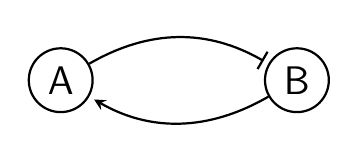
\begin{tikzpicture}	[node distance=3cm,thick,
	activate/.style={-stealth, shorten >= 2pt},
	repress/.style={-|, shorten >= 2pt},
  main node/.style={circle,fill=white,draw,font=\sffamily\Large}]

\node[main node] (1) {A};
\node[main node] (2) [right of=1] {B};
\draw[repress] [bend left] (1) to (2) {};
\draw[activate] [bend left] (2) to (1) {};
\end{tikzpicture}
\caption[A graphical representation of a biochemical system]{A graphical representation of a biochemical system. The two nodes, A and B represent species and the edges (arrows) a reaction between the two. An arrow represents activation and a flat line represents repression.}
\label{fig:Toggle_switch_example}
\end{center}

\end{figure}	



\subsubsection{\acrfull{sbml}}

The \acrfull{sbml} was developed by~\textcite{Hucka:2003wg} in order to allow for the exchange of biochemical models between software. It is an extension of the XML encoding~\autocite{DuCharme:1999} with additional fields specific to biochemical models. Software like Copasi~\autocite{Hoops:2006gy} can be used to convert a set of coupled chemical reactions to an SBML model. SBML models have been a key resource for model sharing within the systems biology community~\autocite{Wilkinson:2006td} in databases like the BioModels database~\autocite{LeNovere:2006ep}. 

\subsection{Transcriptional binding kinetics}

The processes of transcription regulation in prokaryotes are complex and there have been a number of mathematical descriptions developed to approximate the dynamics observed. These include the Hill equation and the Shea-Ackers formalism. 

\subsubsection{Hill formalism}
\label{sec:hill}
The Hill formalism is often used to describe a biochemical system where an activator or repressor is present~\autocite{Hill:1910vo}. The Hill function is often represented as

\begin{align*}
	\frac{dP}{dt} = V_{max}\frac{x^n}{1 + x^n},
\end{align*}
\noindent if activation is being modelled. This is an increasing S-shaped function. Parameter $n$ is the Hill coefficient and $K$ the dissociation constant. $V_{max}$ is the maximum amount of product and $x = \frac{S}{K}$, where S is the substrate concentration. The Hill function reaches a plateau at high substrate concentrations, as is often seen in biological reactions~\autocite{Alon:2007}. $K$ represents the substrate concentration that results in half of the response and the Hill coefficient affects the steepness of the function and represents the cooperativity of the binding to the promoter~\autocite{Alon:2007}. If repression is being modelled, the Hill function is represented as

\begin{align*}
	\frac{dP}{dt} = V_{max}\frac{1}{1 + x^n}.
\end{align*}



\noindent An example of the effect that the value of the Hill coefficient $n$ has on the shape of the Hill function in both activation and repression is given in Figure~\ref{fig:hill_ex}. The higher the value of $n$, the more step-like the function becomes~\autocite{Alon:2007}. 
\newpage

\begin{figure*}[htb]
\centerfloat
    \includegraphics[scale=0.6]{../../chapters/chapterBackgr/images/hill_both-01.png}
    \caption[Hill formalism example]{The effect of different values of $n$ on the Hill function when $K$ is kept constant in the case of (A) activation and (B) repression.}
    \label{fig:hill_ex}
\end{figure*}



\subsubsection{Shea-Ackers formalism}
\label{sec:shea-ackers}
The Shea-Ackers formalism developed by~\textcite{Ackers:1982tq} uses a statistical thermodynamic model to represent the binding of transcription factors to their promoters. A system is described by the various states the promoter can have. An example of possible states is given in Figure~\ref{fig:shea_ack_ex}. Each state has an associated term, or weight, and the probability of transcription is given by the ratio of the producing states over all possible states. This is referred to as the partition function. 

\begin{figure*}[htb]
\centerfloat
    \includegraphics[scale=0.8]{../../chapters/chapterBackgr/images/shea-ackers.png}
    \caption[Shea-Ackers formalism example]{An example of a promoter regulated by a repressor (R) and an activator (A) modelled using the Shea-Ackers formalism. Figure adapted from~\textcite{Woods:2016eh}}
    \label{fig:shea_ack_ex}
\end{figure*}


\begin{align}
	P_{T} = \alpha \frac{k_1 + k_{3}A^2}{1 + k_1 + k_{2}R^2 + k_{3}A^2}.
\end{align}
Here I assume that repression and activation is cooperative, thus two transcription factors must bind to the promoter to repress or activate it. 
\newpage
\subsection{Simulation of deterministic dynamical systems}
Deterministic modelling utilises \acrfull{ode}s and models the concentrations of the species (proteins or other molecules) by time-dependent variables~\autocite{deJong:2002ft}. Rate equations are used to model gene regulation where the rate of production of a species is a function of the concentrations of the other species~\autocite{deJong:2002ft}. 

\subsubsection{Deterministic mass action kinetics}
\label{sec:predator_prey_odes}
\acrshort{ode}s are used to represent the quantitative dynamics of a biochemical network. The \acrshort{ode}s describing a system can be derived from the coupled chemical reactions describing the system as well as their associated rates. This will be illustrated using a simple example, the Lotka-Voltera predator-prey model~\autocite{lotka:voltera}. This system describes the dynamics between two interacting species, a predator and a prey. The chemical reactions describing the system are given in Table~\ref{tab:pp_reac}. The rates of the system are organised in vector form,


\begin{table}[h]
\centering
\caption{Predator-prey chemical reactions}
\label{tab:pp_reac}
\begin{tabular}{@{}lll@{}}
\toprule
Name & Reaction & Rate \\ \midrule
prey birth & $x \xrightarrow{k_1} 2x$ & $k_{1}x$ \\
predation & $x + y \xrightarrow{k_2} 2y$ & $k_{2}xy$ \\
predator death & $y \xrightarrow{k_3} \varnothing$ & $k_{3}y$ \\ \bottomrule
\end{tabular}
\end{table}

\begin{align*}
h = 
\begin{pmatrix}
	k_{1}x \\
	 k_{2}xy \\
	 k_{3}y 
\end{pmatrix}.
\end{align*}
The stoichiometry matrix of the system is an $m\times n$ matrix, where $m$ is the number of species and $n$ the number of reactions and it summarises the stoichiometries of the system, 
\begin{align}
S = \begin{pmatrix}
	1 & -1& 0\\
	0&1&-1 
\end{pmatrix}.
\end{align}
The \acrshort{ode}s can then be constructed by multiplying the stoichiometry matrix $S$ by the matrix containing the rates $h$. Therefore
\begin{align}
s(t) = \frac{d}{dt}\begin{pmatrix}
x\\
y 
\end{pmatrix} = \begin{pmatrix}
1 &-1  &0 \\ 
 0&1  &-1 
\end{pmatrix}\begin{pmatrix}
k_1[x]\\
k_2[x][y]\\
k_3[y] 
\end{pmatrix},
\end{align}
and thus we get the two \acrshort{ode}s describing the system as

\begin{align}
\frac{dx}{dt} &= k_1x - k_2xy\\ \label{eq:predator-prey}
\frac{dy}{dt} &= k_2xy - k_3y.
\end{align}

\noindent These differential equations can be simulated numerically over time using software packages like Mathematica~\autocite{mathematica:2016} and Python.

\subsubsection{Assumptions of deterministic modelling}

Two key assumptions are made when modelling a biochemical system using \acrshort{ode}s. Firstly, the species present in the system are measured continuously rather than discretely. This means that the species are measured in concentration over time and not the number of molecules over time. This assumption requires a large number of molecules to be present in order to be met~\autocite{iglesias:2010}. The second assumption made is that the reactants are in a well-mixed solution. This means that the species in the system can interact each other constantly and freely. 


\subsection{Nonlinear dynamical modelling}

\subsubsection{Phase plane analysis}
An alternative to studying the trajectory of a dynamical system over time is to study its behaviour in the phase plane. During a phase plane analysis the dependent variables $x$ and $y$ are plotted against each other. An example of a phase plane analysis of the predator-prey model given in Equations~\ref{eq:predator-prey} is shown in Figure~\ref{fig:pp_phase}.

\begin{figure*}[htb]
\centerfloat
    \includegraphics[scale=0.7]{../../chapters/chapterBackgr/images/phas_plane_example.png}
    \caption[Phase plane analysis]{The predator-prey system is defined by Equations~\ref{eq:predator-prey}. (A) The trajectory over time (B) Phase plane plot of the predator-prey system of equations. The parameters used here are $k_1=2$, $k_2=1$ and $k_3=1$.}
    \label{fig:pp_phase}
\end{figure*}

\subsubsection{Steady states}

For a system $s$, any point satisfying $\frac{d}{dt}s(t) = 0$ is considered a fixed point, or steady state. At that point the dynamics of the system are considered in equilibrium and will not change with increasing time. Using the example of the predator-prey system, a steady state exists when the system of Equations~\ref{eq:predator-prey} are equal to 0: 
 
\begin{align}
\frac{dx}{dt} &= f_x(x,y) = k_{1}x - k_{2}xy = 0\\
\frac{dy}{dt} &= f_y(x,y) = k_{2}xy - k_{3}y = 0
\end{align}

By solving this system of equations, we get two steady states. One when $x = y = 0$ and one when $x = \frac{k_3}{k_2}$ and $y = \frac{k_1}{k_2}$. The stability of each steady state can then be determined.

\subsubsection{Steady state stability} 

A stable steady state is defined as a fixed point whose nearby points approach the fixed point~\autocite{kaplan:1959}. This means that after a small perturbation the system will quickly return to the steady state. An unstable steady state is one which if the system is perturbed slightly then it moves away from the steady state~\autocite{konopka:2007}. The stability of the fixed points can be determined by the sign of the eigenvalues of the Jacobian matrix at each point. The Jacobian matrix is given by 

\begin{align}
\textbf{J} = \begin{pmatrix}
	\frac{\partial f_x}{\partial x} & \frac{\partial f_x}{\partial y}\\
	\frac{\partial f_y}{\partial x} & \frac{\partial f_y}{\partial y}	
\end{pmatrix}
\end{align}


\noindent Using the predator-prey system as an example, the Jacobian matrix is given by

\begin{align}
\textbf{J} = \begin{pmatrix}
	k_1 - k_{2}y & -k_{2}x\\
	k_{2}y & k_{2}x - k_3 
\end{pmatrix}
\end{align}

\noindent The eigenvalues λ are given by

\begin{align}
\det(\mathbf{J} - λ\mathbf{I}),
\end{align}

\noindent where det is the determinant and \textbf{I} the identity matrix. If both eigenvalues are real and negative or imaginary with a negative real part then the steady state is stable. If both eigenvalues have a positive real part then the steady state is unstable and if one has a positive and one has a negative fixed part the steady state is an unstable saddle node. If both eigenvalues are purely imaginary, the system oscillates around the fixed point. Solving the above for the fixed points in the predator-prey system, we find one stable steady state and one oscillatory fixed point. 


\subsubsection{Bifurcation analysis}

A bifurcation analysis is carried out in order to study the effect that parameters have on the dynamical behaviour of the system~\autocite{Strogatz:1994}. In order to create a bifurcation diagram, all the parameters in the system remain constant while the value of one parameter is varied. We can then observe any changes in the number and stability of the steady states of the system, for example, whether a stable equilibrium in the system becomes unstable. The point where a major change occurs in the steady states of the system is called a bifurcation point~\autocite{iglesias:2010}. The stability of the steady state, as well as its position, is depicted on a bifurcation diagram. By convention, the unstable branches are denoted by a dashed line and the stable branches by a solid line~\autocite{Strogatz:1994}. 

One example of a bifurcation is the saddle-node bifurcation. This occurs when two stable states come closer together until they collide and destroy each other~\autocite{Strogatz:1994}. This can be illustrated using a simple example from \textcite{Strogatz:1994}. Consider the following system 

\begin{align*}
	\frac{dx}{dt} = r + x^2.
\end{align*}

\noindent A bifurcation diagram of the above can be constructed by varying the value of parameter $r$. This gives the bifurcation diagram shown in Figure~\ref{fig:exampl_bifurc}. This system has two steady states when $r$ \textless 0, one unstable steady state and one stable. When $r = 0$ these collapse into one steady state which then disappears when $r$ \textgreater 0. 
\newpage
\begin{figure*}[h]
    \begin{center}
    \includegraphics[scale=0.5]{../../chapters/chapterBackgr/images/example_bifurc.png}
    \caption[Example of a saddle-node bifurcation diagram]{An example of a saddle-node bifurcation diagram. Figure adapted from~\textcite{Strogatz:1994}.}
    \label{fig:exampl_bifurc}
    \end{center}
\end{figure*}




\subsection{Stochastic modelling of dynamical systems}

The assumptions that have to be made to model a system deterministically cannot always be met. This can occur when the molecule numbers in the system are low. When this is the case, stochastic dynamics are more appropriate to model the dynamical system. In stochastic modelling species are measured in discrete amounts rather than concentrations and a joint probability distribution is used to express the probability that at time \textit{t} the cell contains a number of molecules of each species~\autocite{deJong:2002ft,khamash_iglesias:2010}. It takes probabilistic effects into account. 

Biological processes are well known to include randomness. The source of this randomness originates from the random collisions between molecules that govern biological reactions~\autocite{khamash_iglesias:2010}. This randomness affects downstream events and the phenotypic behaviour of cells. This is known as cellular noise and it is known to be key for various cellular processes~\autocite{Eldar:2010kk}. Cellular noise can be classified into two categories, intrinsic noise and extrinsic noise. Intrinsic noise originates from the inherently random collisions between the species of the system under consideration. Extrinsic noise originates from fluctuations in the environment within which the system of interest resides, like the number of available RNA polymerases or other protein numbers~\autocite{khamash_iglesias:2010}. The noisiness of biological processes often makes stochastic dynamics more appropriate for modelling cellular systems.  


%Stochastic modelling is used to describe systems that behave discretely and stochastically~\autocite{Wilkinson:2006td}. It takes into account the randomness in the behaviour of the species involved in a biochemical system, known as 'intrinsic' noise. The probability that a given species will have a certain number of molecules at time t is described by a stochastic simulation~\autocite{khamash_iglesias:2010}.   

\subsubsection{Simulating stochastic models}

Stochastic models are often analytically intractable but can be studied using numerical simulation. A well known algorithm for the simulation of such models is the Direct method proposed by~\textcite{Gillespie:1977ww}.

%Stochastic models can be simulated using a number of different methods. Here I will describe the use of Monte Carlo simulations, as these are used throughout this thesis. The most widely used of the Monte Carlo algorithms is the Gillespie algorithm, described below. 


\subsubsection{The Gillespie algorithm}
 In stochastic systems, the Gillespie algorithm is widely used to simulate the time-evolution of the state of the system~\autocite{Wilkinson:2006td}. The algorithm, developed by~\textcite{Gillespie:1977ww} can be summarised in four steps:
%What type of random numbers are generated for each of these? How does the time-step one work? (i.e. is there a limit on the length of timestep that can be produced?)
\begin{enumerate}
\item Initialise time $t$ and number of species $s$ and state of system $x$
\item Draw a sample time step τ from the (exponential) distribution of time $Τ$
\item Draw a sample reaction from all reactions $R$
\item Update time by $t = t + τ$ and state of system by $x = x + s_μ$
\item Repeat from Step 2 until total simulation time reached
\end{enumerate}
   
\noindent This algorithm results in one trajectory of the system. It has to be repeated a number of times to obtain enough realisations of the trajectory to compute appropriate summary statistics.

\subsubsection{Stochastic mass action kinetics}
Here I will consider the predator-prey system introduced in Section~\ref{sec:predator_prey_odes}. A set of reactions is defined, as shown in Table~\ref{tab:pp_reac}, and each one has an associated stochastic rate constant $c_i$. The rate constant, or hazard function, of each reaction $i$ is defined as $h_i(x, c_i)$, where x is the current state of each species in the system. The form of each hazard function is defined by the order of the given reaction~\autocite{Wilkinson:2006td}, as shown in Table~\ref{tab:hazards}. When simulating a stochastic system using the Gillespie algorithm, the state of the system $x$ is defined as the sum of all the reaction hazards, namely $h_0(x, c) = \sum_{i=1}^{n}h_{i}(x, c_i)$~\autocite{Wilkinson:2006td}. 



\begin{table}[h]
\centering
\caption{Defining reaction hazards}
\label{tab:hazards}
\begin{tabular}{@{}lll@{}}
\toprule
Order & Reaction & Hazard \\ \midrule
Zeroth & $\varnothing \xrightarrow{c_i}X $ & $h_i(x, c_i) = c_i$ \\
First & $X_a \xrightarrow{c_i} ? $ & $h_i(x, c_i) = c_{i}x_a$ \\
Second & $X_a + X_b \xrightarrow{c_i} ? $ & $h_i(x, c_i) = c_{i}x_{a}x_b$ \\
Dimerization & $X_a + X_a \xrightarrow{c_i} X_{2a} $ & $h_i(x, c_i) = c_{i}\frac{x_{a}(x_{a}-1)}{2}$ \\ \bottomrule
\end{tabular}
\end{table}


\section{The Bayesian approach to parameter inference and system design}

%For a model to be used in a systems biology setting the parameters must first be defined. 
The parameters of a model represent the biochemical rates that are involved in the system under study, like degradation rates, transcription rates and polymerization rates. These rates cannot often be measured \textit{in vitro} and taking generalised estimates from existing literature can be inaccurate. In order to make useful predictions about the biological system under consideration, the model parameters must be estimated~\autocite{Zheng:2010bp}. 

To address this challenge, statistical optimisation methods have been developed. These methods aim to infer the parameters of the model that can give rise to some experimentally observed behaviour. Parameter inference methods have the same general structure: there is a cost function that compares the model data to the experimental data and an optimisation function that aims to optimize the cost function~\autocite{Toni:2010}. There is a wide range of such optimisation algorithms that can be used like gradient descent~\autocite{Levenberg:1944we, Marquardt:1963wr}, simulated annealing~\autocite{Kirkpatrick:1983kv} and evolutionary algorithms~\autocite{Onbasoglu:2001um, Wood:2002uo}.  

Bayesian approaches to parameter inference have been shown to work well in biological problems~\autocite{Barnes:2011hh, Toni:2010, Liepe:2014iw}. Bayesian approaches to parameter inference have the advantage of offering a range of values that give rise to the data, rather than point estimates. In Bayesian approaches the aim is to obtain the posterior distribution, which is dependent on the prior distribution, the prior knowledge about the system, and the likelihood, which is obtained from the data. At the core of Bayesian statistics lies Bayes' rule which states that, for a set of data $x$ and a model with a set of parameters $θ$:

\begin{align}
	p(θ|x) = \frac{p(x|θ)p(θ)}{p(x)} \propto p(x|θ)p(θ), \label{eq:bayes}
\end{align}



\noindent where $p(x|θ)$ is the likelihood, and $p(θ)$ is the prior. In continuous problems, Equation~\ref{eq:bayes} becomes

\begin{align}%
	p(θ|x) &= \frac{p(θ)p(x|θ)}{\int p(x|θ)p(θ)dθ}
\end{align}


\noindent where $\displaystyle \int p(x|θ)p(θ)dθ$ is the evidence. It is often not possible to obtain analytical expressions of the posterior, but methods to approximate it numerically have been developed~\autocite{Barnes:2011bk}. One such class of algorithms are the Markov Chain Monte Carlo methods~\autocite{Gilks96}. These are described in more detail in Section~\ref{sec:abc}.


Parameter estimation problems typically involve a set of observed data and a mathematical model describing the biological system. Oftentimes there are a number of competing models under consideration. The challenge then is to fit the model, and model parameters in order to reconstruct the observed data~\autocite{Ma:2009ig}. In system design a different but related problem must be addressed; Instead of experimental data the researcher has an idea of what the system output should be~\autocite{Barnes:2011bk}. A set of carefully selected design objectives can then be used as substitute data ($x_s$), representing data one would like to observe, in the Bayesian inference problem~\autocite{Barnes:2011bk}. This method has been successfully applied in synthetic biology system design~\autocite{Barnes:2011hh, Woods:2016eh}. 

%These optimisation methods can largely be separated into two categories: frequentist and Bayesian. Frequentist methods provide point estimates of the inferred parameters, with associated confidence intervals. On the other hand Bayesian methods offer probability distributions over the values of the inferred parameters. These are especially suited for use in synthetic biology problems, where the  
%In this section I aim to discuss the use of Bayesian methods for parameter inference and system design.  
%All methods are comprised largely of a cost function that compares the model data to the experimental data and an optimisation function that aims to optimize the cost function. There is a wide range of such optimisation algorithms used like gradient decent(XXX), simulated annealing(XXX) and evolutionary algorithms(XXX). 



 







%\section{Introduction to Bayesian statistics}
%\subsection{Bayes' theorem}
%\subsection{Bayesian inference}
%\subsection{Model checking}
%\subsection{Prior selection}

%\subsection{Parametric robustness defined via Bayesian statistics}
%
%\begin{align*}
%p(\theta|x) &= \frac{p(x|\theta)p(\theta)} {\displaystyle \int p(x|\theta)p(\theta)d\theta\frac{p(x|\theta)p(\theta)}{p(x)}}
%\end{align*}
%
%because
%\begin{align*}
%p(x)p(\theta|x) &= p(\theta)p(x|\theta)
%\end{align*}
%
%where $p(x|\theta)$ is the likelihood, $p(\theta)$ is the prior, and $\displaystyle \int p(x|\theta)p(\theta)d\theta$ is the evidence. This is the normalisation. 
%
%Bayes factor: 
%\begin{align*}
%B_{12} = \frac{\displaystyle \int p(x|\theta, M_1)p(\theta, M_1)d\theta}{\displaystyle \int p(x|\theta, M_2)p(\theta, M_2)d\theta}
%\end{align*}
%
%
%In our case, O is the objective, and D is the design. Therefore:
%
%\begin{align*}
%p(O|D_1) = \int p(O|\theta,D_1)p(\theta|D_1)d\theta,
%\end{align*}
%
%
%
%This is the robustness, or evidence or marginal likelihood
%
%\begin{align*}
%p(O|D_1) &= \displaystyle \int p(O|\theta,D_1)p(\theta|D_1)d\theta, \\
%p(O|D_1) &= \displaystyle \iiint_{\underline{\Theta}} p(O|\underline{\Theta})p(\underline{\Theta}|D_1)d\underline{\Theta}
%\end{align*}
%
%where $\underline{\Theta} = \{ \theta_1, \theta_2,\theta_3 \}$ 
%
%Assuming the prior is uniform, and $a=0$:
%
%\begin{align*}
%p(O|D_1) &= \displaystyle \iiint_{\underline{\Theta}} p(O|\underline{\Theta})\frac{1}{b_1}\frac{1}{b_2}\frac{1}{b_3}d\underline{\Theta} \\
%p(O|D_1) &= \frac{1}{b_1}\frac{1}{b_2}\frac{1}{b_3} \displaystyle \iiint_{\underline{\Theta}}p(O|\underline{\Theta})d\underline{\Theta}
%\end{align*}
%
%
%Assuming uniform likelihood:
%\begin{align*}
%p(O|D_1) &= \frac{1}{b_1}\frac{1}{b_2}\frac{1}{b_3} \displaystyle \iiint_{\underline{\Theta}_F}1d\theta_1\theta_2\theta_3+\frac{1}{b_1}\frac{1}{b_2}\frac{1}{b_3} \displaystyle \iiint_{\underline{\Theta}_F}Od\underline{\Theta}
%\end{align*}
%
%


%\section{Background}
%behind making a bistable switch, as well as those necessary to make a tristable switch. %We find that degradation rates of transcription factors are important for bistability, and that the addition of positive autoregulation can create tristable behaviour and also significantly more robust bistability when feedback strength is well balanced. Modelling transcription and translation allows us to conclude that transcriptional bursting can inhibit bistability, and also that bistability can occur even when the assumptions of time scale separation in the repressor dynamics are not met. We also examine the design principles behind the design of bistable versus tristable switches and highlight the importance of including stochastic dynamics when modelling these systems. Finally we demonstrate the ability of the framework to examine more complex systems and examine the design principles of a three gene switch. These examples demonstrate that StabilityFinder will be a valuable tool in the future design and construction of novel gene networks. 
\subsection{\acrfull{abc}}
\label{sec:abc}
%\subsection{\acrshort{abc} algorithms}

%Stability Finder is based on a statistical inference method which combines \acrshort{abc} with \acrfull{smc}~\autocite{Toni:2009tr}. This simulation-based method uses an iterative process to arrive at a distribution of parameter values that can give rise to observed data or a desired system behaviour~\autocite{Barnes:2011hh}.

ABC methods are used for inferring the posterior distribution in cases where it is too computationally expensive to evaluate the likelihood function. Instead of calculating the likelihood, ABC methods simulate the data and then compare the simulated and observed data through a distance function~\autocite{Toni:2009tr}. Given the prior distribution $p(\theta)$ we can approximate the posterior distribution, $p(\theta\mid x)\propto p(x\mid\theta)p(\theta)$, where $p(x\mid\theta)$ is the likelihood of a parameter, $\theta$, given the data, $x$. There are a number of different variations of the ABC algorithm depending on how the approximate posterior distribution is sampled. 

The simplest \acrshort{abc} algorithm is the \acrshort{abc} rejection sampler~\autocite{Pritchard:1999td}. In this method, parameters are sampled from the prior and data simulated through the data generating model. For each simulated data set, a distance from that of the data is calculated, and if greater than a threshold, \textepsilon{}, the sample is rejected, otherwise it is accepted. 
\begin{algorithm}[H]

  \caption{ABC rejection algorithm}
 	\label{alg:ABC}
 \begin{algorithmic}[1]
    \Statex
	\State Sample a parameter vector \texttheta{} from prior $p(\theta)$
	\State Simulate the model given \texttheta{}
    \State Compare the simulated data with the desired data, using a distance function d and tolerance \textepsilon{}. if d $\leq$ \textepsilon{}, accept \texttheta{} 
   
  \end{algorithmic}
\end{algorithm}


\noindent The main disadvantage of this method is that if the prior distribution is very different from the posterior, the acceptance rate is very low~\autocite{Toni:2009tr}. An alternative method is the \acrshort{abc} \acrfull{mcmc} developed by~\textcite{Marjoram:2003up}. The disadvantage of this method is that if it gets stuck in an area of low probability it can be very slow to converge~\autocite{Sisson:2007il}. 

An alternative method developed by~\textcite{Toni:2009tr} takes advantage of \acrlong{smc}, and avoids issues faced by the rejection and \acrshort{mcmc} methods. It propagates the prior through a series of intermediate distributions in order to arrive at an approximation of the posterior. The tolerance, ε, for the distance of the simulated data to the desired data is made smaller at each iteration. When ε is sufficiently small, the result will approximate the posterior distribution~\autocite{Toni:2009tr}.  

%The desired behaviour of the system is used as the data to which the candidate model output is compared to \cite{Barnes:2011hh}. 
%Given a set of competing models, their associated prior estimates of their parameters and the design specifications, the algorithm is able to rank the models according to how well they describe the data and the posterior probabilities of the parameters \cite{Barnes:2011hh}. 

ABC SMC can identify the parameter values within a predefined range of values that can give rise to the data. It works by first sampling at random from the initial range set by the researcher, i.e. from the prior distribution of values. Each sample is called a particle. It then simulates the model given those values and compares that to the target behaviour. If the distance between the simulation and the target behaviour is greater than a predefined threshold distance ε, then the parameter values that produced that simulation are rejected. This is repeated for a predefined number of samples which are collectively referred to as a population. Each particle in a population has a weight associated with it, which represents the probability of it producing the desired behaviour. At subsequent iterations, the new samples are obtained from the previous populations and the ε is set to a smaller value, thus eventually reaching the desired behaviour. The algorithm proceeds as follows:

\begin{algorithm}[H]

  \caption{ABC SMC algorithm}
	\label{alg:ABC-SMC}
 \begin{algorithmic}[1]
    \Statex
    \State Select ε and set population t = 0
	\State Sample particles (θ). If t = 0, sample from prior distributions (p). If t $\textgreater$ 0, sample particles from the previous population to obtain θ*.
	\State If t $\textgreater$ 0: Perturb each particle θ* using perturbation kernel $K_t$ to obtain perturbed particle θ** %, by $\pm$ half the range of the previous population (j) to obtain new perturbed population (i).
	\State Simulate each particle to obtain time course.
	\State Reject particles if d $\textgreater$ ε.
	\State Calculate the weight $w$ for each accepted particle. At the first population assign a weight equal to 1 for all particles. In subsequent populations the weight of a particle is equal to the probability of observing that particle divided by the sum of the probabilities of the particle arising from each of the particles in the previous population:

	\State $w_{t}^{(i)} = \begin{cases} 1, & \mbox{if } t = 0 \\\frac{p(\theta_{t}^{(i)})}{\sum_{j=1}^N w_{t-1}^{(j)} K_{t}(\theta_{t-1}^{(j)}, \theta_{t}^{(i)})}, & \mbox{if } t $\textgreater$  0. \end{cases}$

  \end{algorithmic}
\end{algorithm}

\noindent Details about each module of the ABC SMC algorithm are given in the sections below. 


\subsubsection{Particle sampling}
\label{sec:part_samp}
For the first population, particles are sampled from the prior, which consists of the boundaries of a distribution for each parameter defined by the user based on biochemical knowledge or literature. For subsequent populations, particles are sampled from the previous population. The weight of each particle in the previous population dictates the probability of it being sampled. The number of samples to be drawn is specified by the user.  

\subsubsection{Perturbation}
\label{sec:pertub}
Each sampled particle is perturbed by a kernel defined by the distribution of the previous population, as developed by~\textcite{Toni:2009tr}. 
\begin{align}
K_t(\theta|\theta^* ) = \theta^* + U(+s_p, -s_p),
\end{align}
\noindent  where
\begin{align}
s_p = \frac{1}{2} \big (max(\theta_{p-1}) - min(\theta_{p-1}) \big )
\end{align}

\noindent If the θ** falls out of the limits of the priors then the perturbation is rejected and repeated until an acceptable θ** is obtained. This method is successful in perturbing the particles by a small amount in order to explore the parameter space, but can be slow to complete. 


\subsubsection{Epsilon schedule}
The algorithm uses an automated epsilon schedule, where the threshold of the next iteration is chosen from the range of values of the current population. This method is the quantile method. Another approach to the epsilon schedule is to use an adaptive epsilon schedule which is efficient in avoiding local minima~\autocite{Silk:2013bi}. Throughout this thesis, the quantile method was used with a tight quantile (0.3) to avoid the problem of local minima. 

\subsubsection{Particle simulation}
\label{sec:sim}
Each particle is simulated using cuda-sim~\autocite{Zhou:2011hp}. The model is provided by the user in SBML format and is converted into CUDA\textsuperscript{\textregistered} code by cuda-sim. The model in CUDA\textsuperscript{\textregistered} code format can then be run on NVIDIA\textsuperscript{\textregistered} \acrshort{gpu}s. This allows the user to take advantage of the speed of parallelised simulations without any CUDA\textsuperscript{\textregistered} knowledge. 


\subsubsection{Weight calculation}
\label{sec:weight}
For the first population the weights are all given a value of 1, and then normalised over the number of particles. For subsequent populations, the weights of the particles are calculated by considering the weights of the previous population~\autocite{Toni:2009tr}. The weights are then normalised over the total number of particles. 


\begin{align}
w_{t}^{(i)} = \frac{p(\theta_{t}^{(i)})}{\sum_{j=1}^N w_{t-1}^{(j)} K_{t}(\theta_{t-1}^{(j)}, \theta_{t}^{(i)})} \text{ for n $\textgreater$  0}.
\end{align}
	
	
\subsubsection{ABC SMC algorithm example}	
This algorithm is implemented on a simple example for illustration. A simple model was used, consisting of one species, $A$ converting to another, $B$. The model is described by two differential equations, where $A$ is the reactant and B the product, produced at a rate $p$. 

\begin{align}
\frac{d[B]}{dt} &= p[A] \\ 
\frac{d[A]}{dt} &= -p[A]. 
\end{align}

\noindent The priors were set to $p \sim U(0, 10)nM s^{-1}$. Initial conditions for $A$ and $B$ were set to 1 and 0 respectively. The data to which the model was compared to was generated by simulating the same model with the parameter set to 1, as shown in Figure~\ref{fig:myABC true 1}.

\begin{figure*}[htbp]
    \begin{center}
    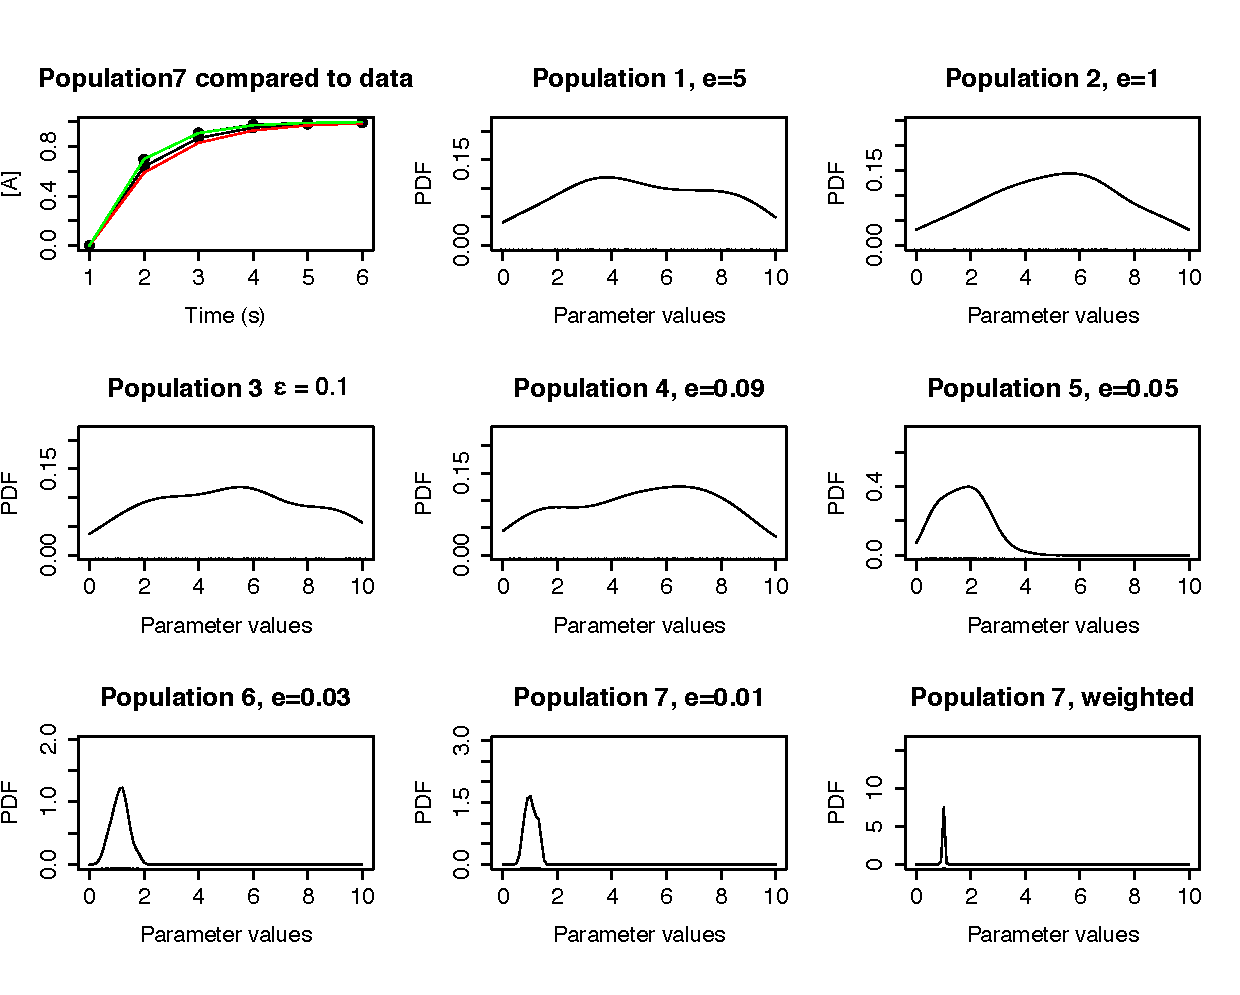
\includegraphics[scale=0.6]{../../chapters/chapterIntroduction/images/abc_smc_example.pdf}
    \caption[\acrshort{abc} \acrshort{smc} parameter inference example]{ABC SMC parameter inference. The true parameter value is equal to 1 and its time course is shown in red in the top left panel. The blue time course is that of the final population, green is the upper quartile and red is the lower quartile range of values. The progress of the selection process can be seen the as the ε schedule proceeds from the top left to the bottom right. The bottom far right panel is a weighted density plot of the posterior distribution of p at ε = 0.01.}
    \label{fig:myABC true 1}
    \end{center}
\end{figure*}


Figure~\ref{fig:myABC true 1} illustrates the use of \acrshort{abc} \acrshort{smc}, using a simple example. During the course of 7 populations, the accepted distance ε of the simulated particles to the data is incrementally decreased. This leads to a final population where the distance of the data to the particles is very small, and there is a good agreement between the two. The algorithm concludes with a set of parameter values that produced this behaviour, which approximate the posterior distribution. The posterior distribution found in this model is in good agreement with the parameter value used to generate the data. 

\clearpage
\subsubsection{Visualising posterior distributions}

The posterior distribution has as many dimensions are there are parameters, thus can be challenging to visualise for models containing more than two parameters. In order to visualise the multi-dimensional posterior distributions in this thesis, the one and two-dimensional marginal distributions of the parameters will be shown. An example of such a plot is shown in Figure~\ref{fig:exampl_post}. The data shown in Figure~\ref{fig:exampl_post} consists of 10000 random samples drawn from a bivariate normal distribution, of mean = 0 for all dimensions and variance σ
\begin{align*}
σ = \begin{bmatrix}
1 &0.5 \\ 
 0.5& 1  
\end{bmatrix}.
\end{align*}
\noindent The two-dimensional distribution is plotted as shown in Figure~\ref{fig:exampl_post}.

\begin{figure*}[h]
    \begin{center}
    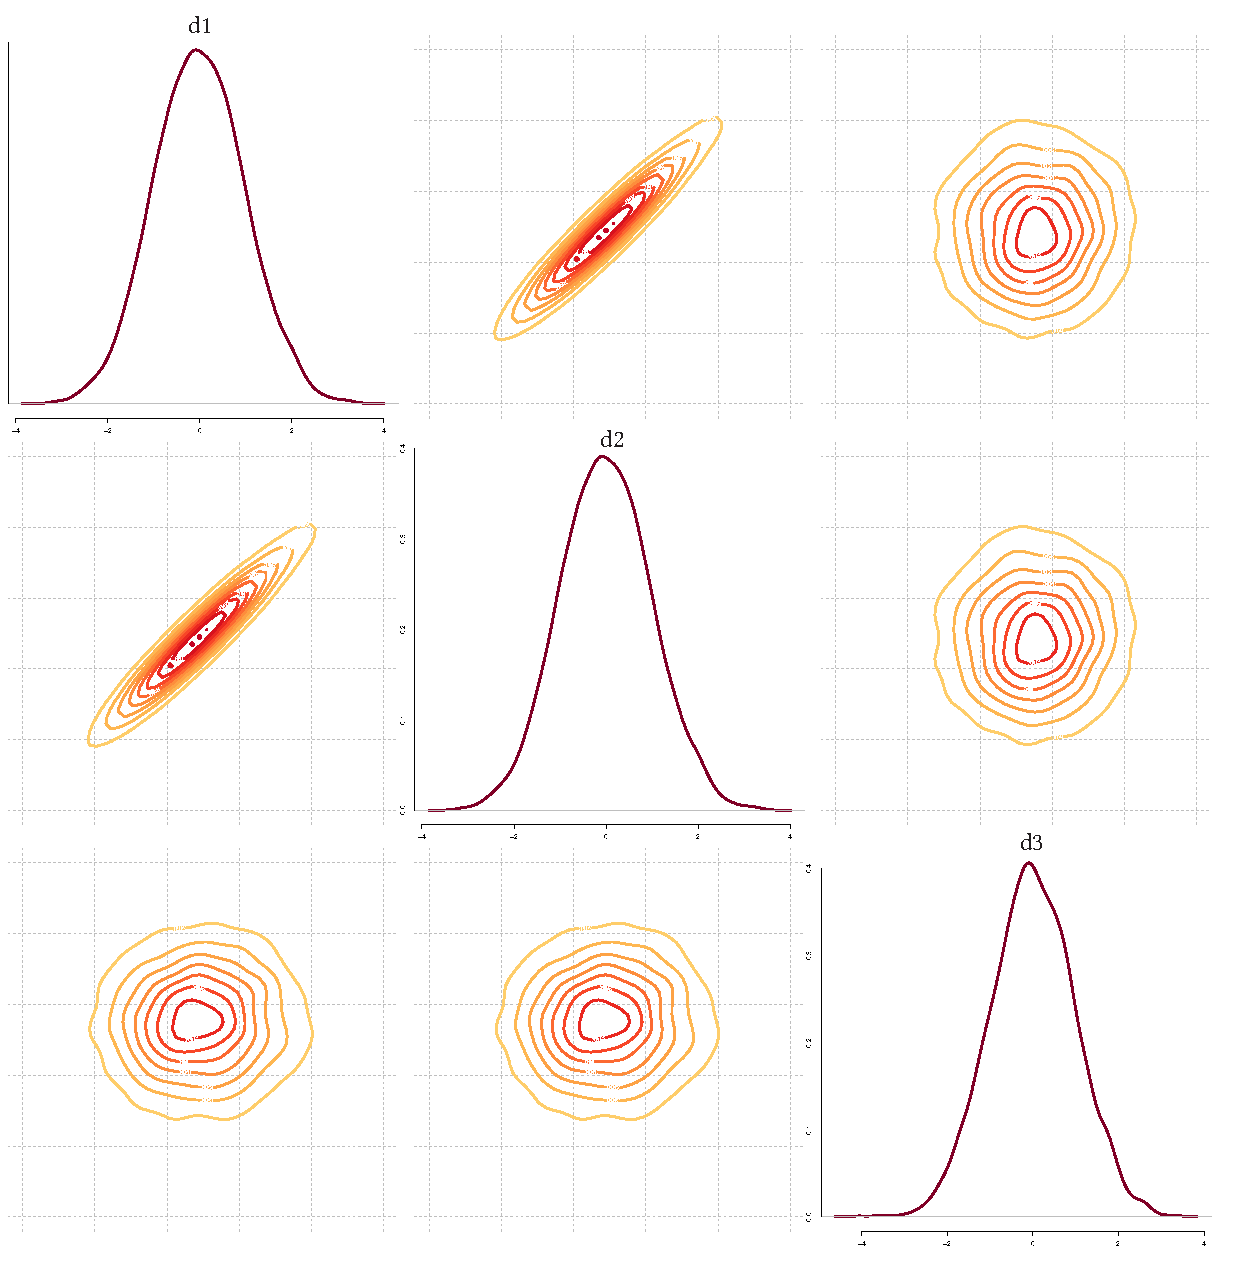
\includegraphics[width=1.1\textwidth]{../../chapters/chapterBackgr/images/example_posterior.pdf}
    \caption[Example of a posterior distribution plot]{Visualising a two-dimensional distribution. (A) A bivariate normal distribution plotted in 3D. (B) A bivariate normal can be visualised by plotting the one-dimensional marginal distributions on the diagonal and the two-dimensional marginal distributions are on the off-diagonal. Correlation can be visualised using the 2D marginal distributions.}
    \label{fig:exampl_post}
    \end{center}
\end{figure*}


	


\subsection{Derivation of model parametric robustness defined via Bayesian statistics}
\label{sec:rob_back}
During this thesis I use the term robustness in its parametric meaning, i.e. as the ability of a system to retain its function despite parameter perturbations~\autocite{Stelling:2004wo}. The robustness of biological systems has been studied extensively~\autocite{Barkai:1997cd, Stelling:2004wo, Prill:2005fq, Kim:2006uk, Kitano:2007cp, Hafner:2009ct, Shinar:2010dd, ZamoraSillero:2011jw, Woods:2016eh}. Below I show that the robustness of a model can be calculated by dividing the volume of its functional region by the volume of its priors. Starting with Bayes' rule that:
%. and it is well known that feedback loops can increase the robustness of a system~\autocite{Becskei:2000ft,	 DOYLE:2005ul}. 
\begin{align}
	f(\theta|x) &= \frac{f(\theta)f(x|\theta)}{\int p(x|\theta)p(\theta)d\theta},
\end{align}

\noindent where $x$ is the data, $p(x|\theta)$ is the likelihood, $p(\theta)$ is the prior, and $\displaystyle \int p(x|\theta)p(\theta)d\theta$ is the evidence. The evidence is the normalisation constant so that the distribution integrates to 1. For a given model design $D_1$ and objective O we define the functional region $F$ as the region within the prior where O is satisfied. So within the prior we can assign 1 to any region that falls within $F$ and 0 to any region outside that. 

\begin{align}
p(O|D_1) = \int p(O|\theta,D_1)p(\theta|D_1)d\theta,
\end{align}

\noindent for a design with three parameters this becomes

\begin{align}
p(O|D_1) &= \displaystyle \iiint_{\underline{\theta}} p(O|\underline{\theta})p(\underline{\theta}|D_1)d\underline{\theta},
\end{align}

\noindent where $\underline{\theta}$ is a vector containing the three parameters $ = (\theta_1, \theta_2,\theta_3)$, and each $\theta_i \in \mathbb{R} $. To calculate the robustness, or model evidence, we integrate this with respect to $\underline{\theta}$. We assume  all parameters $\theta_1, \theta_2,\theta_3$ have uniform prior, $p(\underline{\theta}|D_1) \sim U(a, b)$. If we assume a = 0 this integral becomes:

\begin{align}
p(O|D_1) &= \displaystyle \iiint_{\underline{\theta}} p(O|\underline{\theta})\frac{1}{b_1}\frac{1}{b_2}\frac{1}{b_3}d\underline{\Theta} \text{ , and }\\
p(O|D_1) &= \frac{1}{b_1}\frac{1}{b_2}\frac{1}{b_3} \displaystyle \iiint_{\underline{\theta}}p(O|\underline{\theta})d\underline{\theta}, \label{eq:1.6}
\end{align}

\noindent since $\frac{1}{b_1}\frac{1}{b_2}\frac{1}{b_3} $ is a constant. Then assuming that the likelihood is uniform Equation~\ref{eq:1.6} becomes

\begin{align}
p(O|D_1) &= \frac{1}{b_1}\frac{1}{b_2}\frac{1}{b_3} \bigg[\displaystyle \iiint_{\underline{\theta}_F} 1 d\underline{\theta} +\cancelto{0}{\displaystyle \iiint_{\underline{\theta}_{\cancel{F} }} 0 d\underline{\theta}}\bigg],  
\end{align}

\noindent since we assign 1 to any region within $F$ and 0 to any region outside it. This becomes:

\begin{align}
p(O|D_1) &= \overbrace{\frac{1}{b_1}\frac{1}{b_2}\frac{1}{b_3}}^{|P|} \underbrace{\displaystyle \iiint_{\underline{\theta}_F} 1 d\underline{\theta}}_{|F|}, \\
\therefore p(O|D_1) &= \frac{|F|}{|P|},
\end{align}
where |P| is the volume of the prior P and |F| the volume of the functional region F. Therefore, in the case where both the prior and the likelihood are uniform, the robustness $R$ of the design is the ratio of the volumes of the two. If on the other hand we assume the likelihood is multivariate normal, with priors remaining uniform, Equation~\ref{eq:1.6} becomes: 
%normal
%\begin{align*}
%p(O|\underline{\Theta}) = c \times exp\bigg(-\frac{(O-\mu)^2}{2\sigma^2}\bigg)
%\end{align*}



%\begin{align}
%p(O|D_1) &= \frac{1}{|P|}\iiint_{\underline{\Theta}}f(\underline{\Theta};\mu,\Sigma)d\underline{\Theta} \\%, & \parbox[c]{\Sigma = \det(\text{covariance matrix})} \\
%\therefore p(O|D_1) &= \frac{1}{|P|}\underbrace{\times(2\pi)^\frac{k}{2}\times |\Sigma|^\frac{1}{2}}_{|F|} \\
%\therefore p(O|D_1) &= \frac{|F|}{|P|},
%\end{align}

\begin{align}
p(O|D_1) &= \frac{1}{|P|}\iiint_{\underline{\theta}}f(\underline{\theta};\mu,\Sigma)d\underline{\theta} \\%, & \parbox[c]{\Sigma = \det(\text{covariance matrix})} \\
\therefore p(O|D_1) &= \frac{1}{|P|}\underbrace{\frac{2\pi^{\frac{k}{2}}}{k\Gamma(\frac{k}{2})} \Big[ \chi _{k}^{2}(\alpha) \Big]^{\frac{k}{2}} |\Sigma|^\frac{1}{2}}_{\text{The volume of an ellipsoid}} \\
\therefore p(O|D_1) &= \frac{|F|}{|P|}.
\end{align}

%\begin{align}
%	V & = \frac{2\pi^{\frac{k}{2}}}{k\Gamma(\frac{k}{2})} \Big[ \chi _{k}^{2}(\alpha) \Big]^{\frac{k}{2}} |\Sigma|^\frac{1}{2}, \label{eq:el_vol}
%\end{align}


\noindent We can use the Bayes factor in order to compare the robustness between two model designs. The Bayes factor is used to determine which model, $M_a$ or $M_b$, can explain the data X better and is defined as follows:

\begin{align}
 B_{12} &= \frac{p(X|M_a)}{p(X|M_b)}, \label{eq:final_bayes1}
\end{align}	

\noindent which represents the fraction of the evidence supported by model $a$ over the evidence supported by model $b$. The evidence against model $M_b$, and thus in favour of $M_a$, the Bayes factor, can be interpreted as shown in Table~\ref{tab:BAYES_FACTS}. For a comprehensive review on the use of Bayes factors see~\textcite{Kass:1995vb}.


In a system design model, the Bayes factor is used to determine which design, $D_1$ or $D_2$ can fulfil the design objective O better. Therefore,


\begin{align}
B_{12} &= \frac{\displaystyle \int p(x|\theta, D_1)p(\theta, D_1)d\theta}{\displaystyle \int p(x|\theta, D_2)p(\theta, D_2)d\theta} = \frac{p(O|D_1)}{p(O|D_2)}\\
\therefore B_{12} &= \frac{|F_1|}{|P_1|} / \frac{|F_2|}{|P_2|}. \label{eq:final_bayes}
\end{align}

\noindent We can thus use the ratio of the two robustness measures to calculate the Bayes factor. If two models have a different number of parameters, the robustness of the system will only increase if |F| increases by more than the proportion by which |P| increased~\autocite{Woods:2016eh}. A model is penalised for an additional parameter if it does not increase the volume of the functional region by more than the volume that the added parameter added to the prior. This is also true for nested models, where one model is wholly contained in the other. 


\begin{table}[tb]
\centering
\caption{Bayes factor evidence interpretation. Modified from~\textcite{Kass:1995vb}}
\label{tab:BAYES_FACTS}
\begin{tabular}{@{}ll@{}}
\toprule
Bayes factor & Evidence \\ \midrule
1 to 3.2 & Not significant \\
3.2 to 10 & Substantial \\
10 to 100 & Strong \\
\textgreater 100 & Decisive \\ \bottomrule
\end{tabular}
\end{table}





%\section{Flow Cytometry}


%\section{Control theory in systems biology}



%% ABC-SysBio ---------------------------------------%%
\mainmatter*
\chapter{Postive feedback loops can increase the robustness of a genetic toggle switch}
\label{ch:abcsysbio}
\section{Introduction}

In this chapter I aim to find out whether adding feedback loops to the genetic toggle switch increases its robustness to parameter fluctuations. To do this, I use \acrshort{abc} \acrshort{smc} model selection, which is capable of selecting the most robust model for a given model behaviour.

Structurally this chapter is organised as follows: In the first section I examine the genetic toggle switch with no added feedback loops. I use a parameter scan to find the parameter values that make it bistable and then use \acrshort{abc} \acrshort{smc} for parameter inference for a switch-like behaviour. In the following section I examine the effect that the addition of feedback loops to the genetic toggle switch has on its stability, and select the switch architectures that are capable of bistable behaviour. Finally, I use ABC-SysBio model selection to select the most robust model out of the bistable switches.


%First parameter scan in order to determine the parameter values that can produce the desired behaviour. Then ABC parameter estimation to determine whether the models used are capable of the desired behaviour. Finally, I use ABC-SysBio model selection to select the most robust model. 


\section{The genetic toggle switch}
%the following is copy paste from SF:
\textcite{Gardner:2000vha} constructed the first synthetic genetic toggle switch. Their model consisted of two mutually repressing transcription factors, and is defined by the following \acrshort{ode}s:

\begin{align}\label{eq:gards}
\frac{du}{dt} &= \frac{a_1}{1+v^{\beta}} - u \\
\frac{dv}{dt} &= \frac{a_2}{1+u^{\gamma }} - v,
\end{align}

\noindent where \textit{u} is the concentration of repressor 1, \textit{v} the concentration of repressor 2, $a_1$ and $a_2$ denote the effective rates of synthesis of repressors 1 and 2 respectively, β is the cooperativity of repression of promoter 1 and γ of repressor 2. 

First, I study the model given in Equations~\ref{eq:gards} by conducting a bifurcation analysis using the PyDSTool~\autocite{Clewley:2012kj} in order to determine whether it is capable of bistable behaviour. The system has two stable steady states and one unstable steady state when $a_1$ and $a_2$ are set to 10, and β, γ set to 2, as shown in Figure~\ref{fig:Gard_CS}B. The bifurcation analysis shows that by varying the parameter for the effective rate of synthesis of repressor 1 while all other parameters remain constant, the system is bistable when 5 \ge{} $a_1$ \le{} 31.



\begin{figure*}[htbp]
	\begin{center}
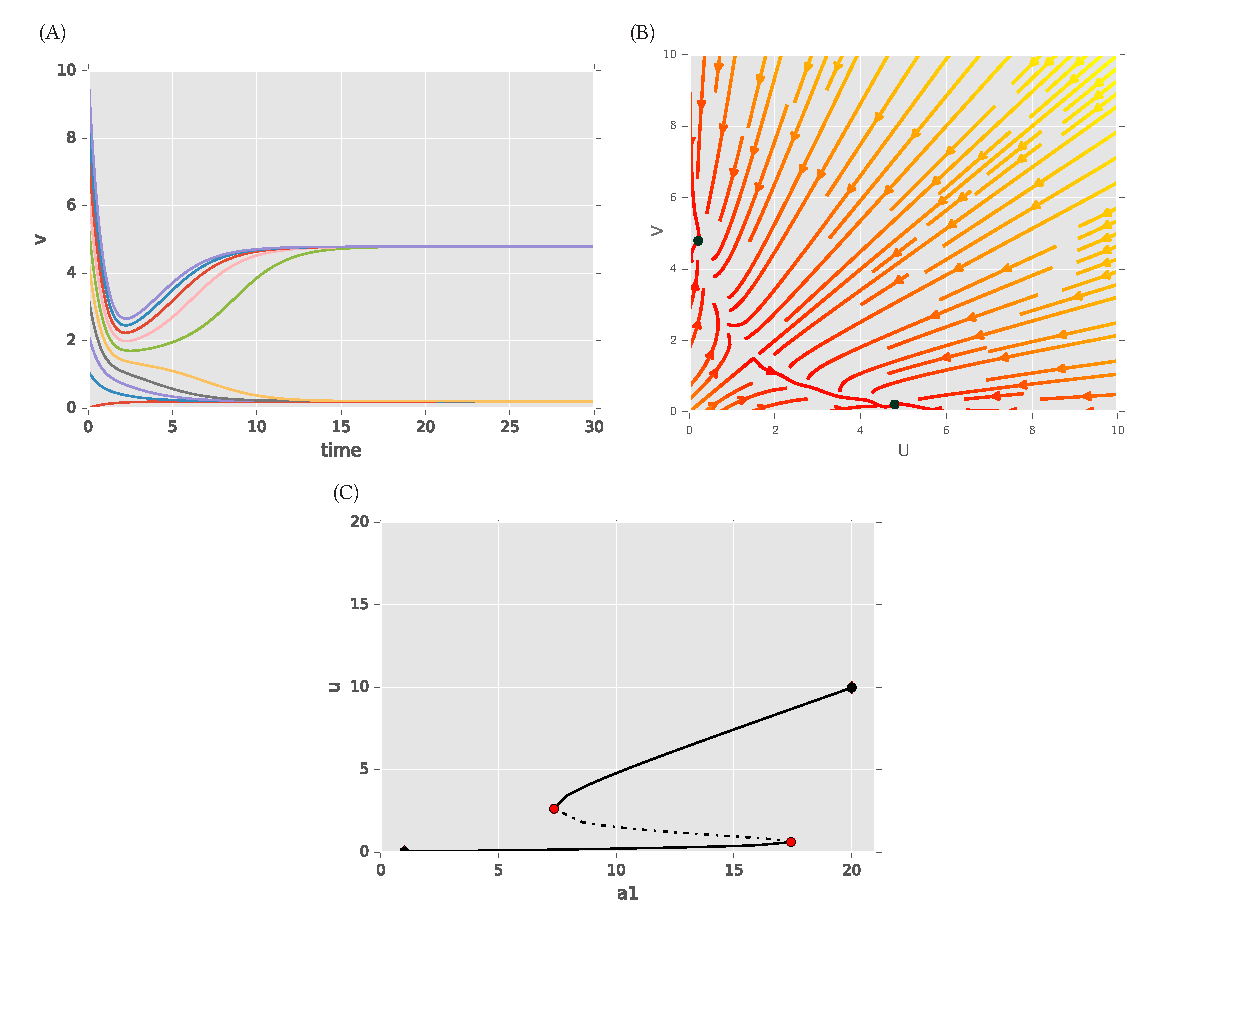
\includegraphics[scale=0.7]{../../chapters/chapterABCSysBio/images/Gard_CS.png}
\caption[LoF caption]{\label{fig:Gard_CS}: The \textcite{Gardner:2000vha} toggle switch is capable of bistable behaviour given $a_1$ and $a_2$ = 10, and β, γ = 2. (A) The timecourse of the simulated model using multiple initial conditions. (B) The vector plot of the Gardner switch shows there are two stable steady states and one unstable steady state. (C) A bifurcation diagram shows that the system is bistable when 5 \ge{} $a_1$ \le{} 31.}
\end{center}
\end{figure*}
\clearpage


\section{Toggle switch parameter scan}
\label{sec:paramscan}
%This bit is from SF chapter as well
In order to study the switch system in a more realistic way, I developed an extension to the ~\textcite{Gardner:2000vha} switch. This new set of switches does not use the \acrfull{qssa} that is often used in modelling the toggle switch. Using mass action, this changes the two-equation system used in Equations~\ref{eq:gards} into a system of 18 equations. The equations describing the system are shown below and illustrated in Figure~\ref{fig:Gard_MA}. The system consists of two genes, gA and gB. The products of the genes homodimerise and mutually repress eachother. There are also two inducers in the system, S and R. S removes AA from the system by binding to the homodimer and thus removes the repression on gene B, and R removes BB from the system by binding to it. A symmetric model, where the parameters for equivalent reactions were set to be the same, was used for simplicity.

\begin{figure*}[tbp]
	\begin{center}
\includegraphics[scale=0.7]{../../chapters/chapterABCSysBio/images/ma-switch-diagram.png}
\caption[LoF caption]{\label{fig:Gard_MA}:An illustration of the model used in the parameter scan. }
\end{center}
\end{figure*}



$$
\begin{array}{cccc}
      \textrm{gA}\stackrel{\textrm{ge}}{\longrightarrow}\textrm{gA} + \textrm{A} \\
      \textrm{gB}\stackrel{\textrm{ge}}{\longrightarrow}\textrm{gB} + \textrm{B} \\
      \textrm{A} + \textrm{A} \stackrel{\textrm{dim}}{\longrightarrow}\textrm{A2} \\
      \textrm{A2} \stackrel{\textrm{dim\_r}}{\longrightarrow}\textrm{A} + \textrm{A} \\
      \textrm{B} + \textrm{B} \stackrel{\textrm{dim}}{\longrightarrow} \textrm{B2} \\
      \textrm{B2} \stackrel{\textrm{dim\_r}}{\longrightarrow}\textrm{B} + \textrm{B} \\
      \textrm{gA} + \textrm{B2} \stackrel{\textrm{rep}}{\longrightarrow}\textrm{B2gA} \\
      \textrm{B2gA} \stackrel{\textrm{rep\_r}}{\longrightarrow}\textrm{B} + \textrm{gA} \\
      \textrm{gB} + \textrm{A2} \stackrel{\textrm{rep}}{\longrightarrow}\textrm{A2gB} \\
      \textrm{A2gB} \stackrel{\textrm{rep\_r}}{\longrightarrow}\textrm{A2} + \textrm{gB} \\
      \textrm{A} \stackrel{\textrm{deg}}{\longrightarrow}\textrm{\O}\\
      \textrm{B} \stackrel{\textrm{deg}}{\longrightarrow}\textrm{\O}\\
      \textrm{S} + \textrm{A2} \stackrel{\textrm{rep\_dim}}{\longrightarrow}\textrm{SA2}\\
      \textrm{SA2} \stackrel{\textrm{rep\_dim\_r}}{\longrightarrow}\textrm{S} + \textrm{A2}\\
      \textrm{R} + \textrm{B2} \stackrel{\textrm{rep\_dim}}{\longrightarrow}\textrm{RB2}\\
      \textrm{RB2} \stackrel{\textrm{rep\_dim\_r}}{\longrightarrow}\textrm{R} + \textrm{B2}\\
      \textrm{R} \stackrel{\textrm{deg}}{\longrightarrow} \textrm{\O}\\
      \textrm{S} \stackrel{\textrm{deg}}{\longrightarrow}\textrm{\O}\\
\end{array}
$$
%This bit is in SF chapter also:
This model is too complex to solve analytically. In order to determine whether it is capable of bistable behaviour, a numerical solution must be deployed. In order to do that I used a parameter scanning algorithm outlined in Algorithm~\ref{alg:param_scan} below. This method involves the scan of parameter values as well as initial conditions for AA and BB. Parameter values are sampled randomly from a uniform distribution. Then for each sample of values, latin hypercube sampling is used to sample initial conditions~\autocite{MCKAY:2000vt}. This is used to ensure that the whole space is sampled uniformly. Latin hypercube sampling is done in two dimensions, in order to sample initial conditions for the two dimers, AA and BB. The uniform priors of the two species in consideration represent a rectangle space, which is subdivided into equal parts. Then a random sample is drawn from each sub-part. This ensures the whole space is evenly sampled. 
\clearpage
\begin{figure*}[tbp]
\begin{center}
\includegraphics[scale=0.5]{../../chapters/chapterABCSysBio/images/LHS.png}
\caption[LoF caption]{\label{fig:lhs}Latin hypercube sampling ensures that the whole space is sampled evenly. For the two species concerned, A and B, we assume uniform distributions, shown in grey. The joint space of the two distributions is divided into smaller equal parts and a random sample is drawn from within each subspace.  }
\end{center}
\end{figure*}


The parameter scan uncovered the presence of tristable, bistable and monostable systems given a different set of parameter values. The Algorithm of the parameter scans is outlined below:
%A deterministic and a stochastic scan were carried out. 


\begin{algorithm}[htbp]
\caption{Parameter scan algorithm}
\label{alg:param_scan}
 \begin{algorithmic}[1]
    \Statex
	\State Select multiple sets of parameter values from a random uniform distribution between 0 and 10.
	\For{each set of parameter values}:
	\State Select multiple sets of initial conditions for the two dimers via latin hypercube sampling
	\For{For each set of initial conditions}
	\State Integrate ODEs of the model
	\State Solve system to steady state
	\EndFor
	\EndFor
  \end{algorithmic} 
\end{algorithm}

One dimer was plotted against the other for all initial conditions of each parameter set. An example for each of the three types of stabilities found during the scan are shown in Figure ~\ref{fig:stab exampl}.

\begin{figure*}[htbp]
\centering
\includegraphics[width=\textwidth]{../../chapters/chapterABCSysBio/images/switch_stbility_examples}
\caption[LoF caption]{\label{fig:stab exampl}: An example for each type of switch found during the parameter scan. Each graph represents the steady state values of one dimer plotted against the other, from one parameter set and 100 initial conditions.}
\end{figure*}



In order to determine which areas in the parameter space give rise to the different kinds of stability, a histogram of the frequency of each parameter value found in monostable, bistable and tristable systems was plotted and shown in Figure~\ref{fig:scan ode param hist}. There were a total of 217 monostable, 16 bistable and 6 tristable switches out of 400 sampled parameter sets. The remaining samples did not reach steady state. This shows that different parameter values have a great effect on the stability profile of the switch.
 
\begin{figure}
\centering
\begin{minipage}[c]{1\textwidth}
\centering
    \includegraphics[width=1.05\textwidth]{../../chapters/chapterABCSysBio/images/param_stability_hist}
    \caption{The distribution of parameter values that resulted in monostable, bistable and tristable switches in the parameter scan. Each graph represents the distribution of the values of one parameter. }
    \label{fig:scan ode param hist}
\end{minipage}
\end{figure}


From the histograms in Figure ~\ref{fig:scan ode param hist} it can be seen that the parameter for gene expression (ge) tends to be relatively high when bistability arises whereas the parameter for the reverse reaction of repression (rep\_r) tends to be low. Degradation (deg) also tends to be low. It must also be noted that the parameter values that give rise to monostable systems are generally evenly distributed for all parameters, suggesting that monostable systems arise from the whole range of values sampled. This can further indicate that the right combination of more than one parameter values is necessary for bistability. 



\section{Toggle switch parameter inference}


In this section I study the problem of how to rationally design a synthetic biological system to perform a behaviour of choice.  In order to address this question I use a Bayesian approach, known as \acrlong{abc} and described in Section(XXX). This approach is capable of approximating the posterior distribution that gives rise to the behaviour of choice~\autocite{Toni:2009tr}. By simulating the model in question, this approach can identify an approximate posterior distribution via a series of intermediate distributions. Here I use an implementation of the above approach, the software package ABC-SysBio~\textcite{Liepe:2010eg}. This method can be used for the rational design of synthetic biological systems by defining some design objectives to which the model is fitted to~\textcite{Barnes:2011hh}. By specifying the inputs to the system and the outputs required, the posterior of the model that can produce this behaviour can be identified. 

This method is used here to fit the model used in Section~\ref{sec:paramscan} to a switch-like behaviour. The design specifications are shown in Figure~\ref{fig:abc_behav}. The two inducers, S and R, as used as inputs to flip the switch ON and OFF respectively. The required output is the switch flipping from the OFF state to the ON state and then to the OFF state again. As priors to the parameter inference I used the parameter values shown to produce a bistable switch in Section~\ref{sec:paramscan}. The priors used are shown in Table~\ref{tab:param_inf_params}.

\begin{table}[htbp]
\centering
\caption{The parameter priors used for the standard toggle switch parameter inference. The priors consist of the lower and upper limit of a uniform distribution}
\label{tab:param_inf_params}
\begin{tabular}{ccccccccc}
\toprule
 \textbf{ge}     & \textbf{rep}     & \textbf{rep r}     & \textbf{dim}    & \textbf{dim r}     & \textbf{deg}  & \textbf{rep dim}    & \textbf{rep dim r} & \textbf{deg sr}    \\
6 9     & 4 10    & 1 4       & 4 10   & 2 7       & 2 5  & 0.05 0.1   & 0.01 0.05     & 0.01 0.05         \\ \bottomrule
\end{tabular}
\end{table}


\begin{figure*}[htbp]
	\begin{center}
\includegraphics[scale=0.7]{../../chapters/chapterABCSysBio/images/behaviour.png}
\caption[LoF caption]{\label{fig:abc_behav}: Design specification for ABC parameter inference. The input to the system consists of an event turning on the stimulus (S) at t=20 and another turning on the repressor (R) at t=70. The output specification is the response to the switch to these stimuli.}
\end{center}
\end{figure*}
In order to fit the switch model to the behaviour specified above, a distance function must be defined. The distance function defines the quantity that is minimized at each successive iteration of \acrshort{abc} \acrshort{smc}. The distance function defined here is shown in Equations\ref{eq:dist}. Three distances are measured, one for each state of the switch, OFF-ON-OFF.


\begin{align}\label{eq:dist}
	d_1 &= \sum_{i=0}^{20} (s_i-t_1)^2 \\
	d_2 &= \sum_{i=21}^{70} (s_i-t_2)^2 \\
	d_3 &=  \sum_{i=71}^{100} (s_i-t_3)^2,
\end{align}
where $i$ represents the timepoints, $s_i$ the simulation result at  each timepoint and $t1 = 0$, $t2 = 20$, $t3 = 0$ represent each target behaviour.


The result of the toggle switch parameter inference are shown in Figure~\ref{fig:stand_abc_timeseries}. The results show that the model can indeed behave like a switch within the parameter range given as priors. 

\begin{figure}[htbp]
    \centering
    \hspace*{-1cm}
    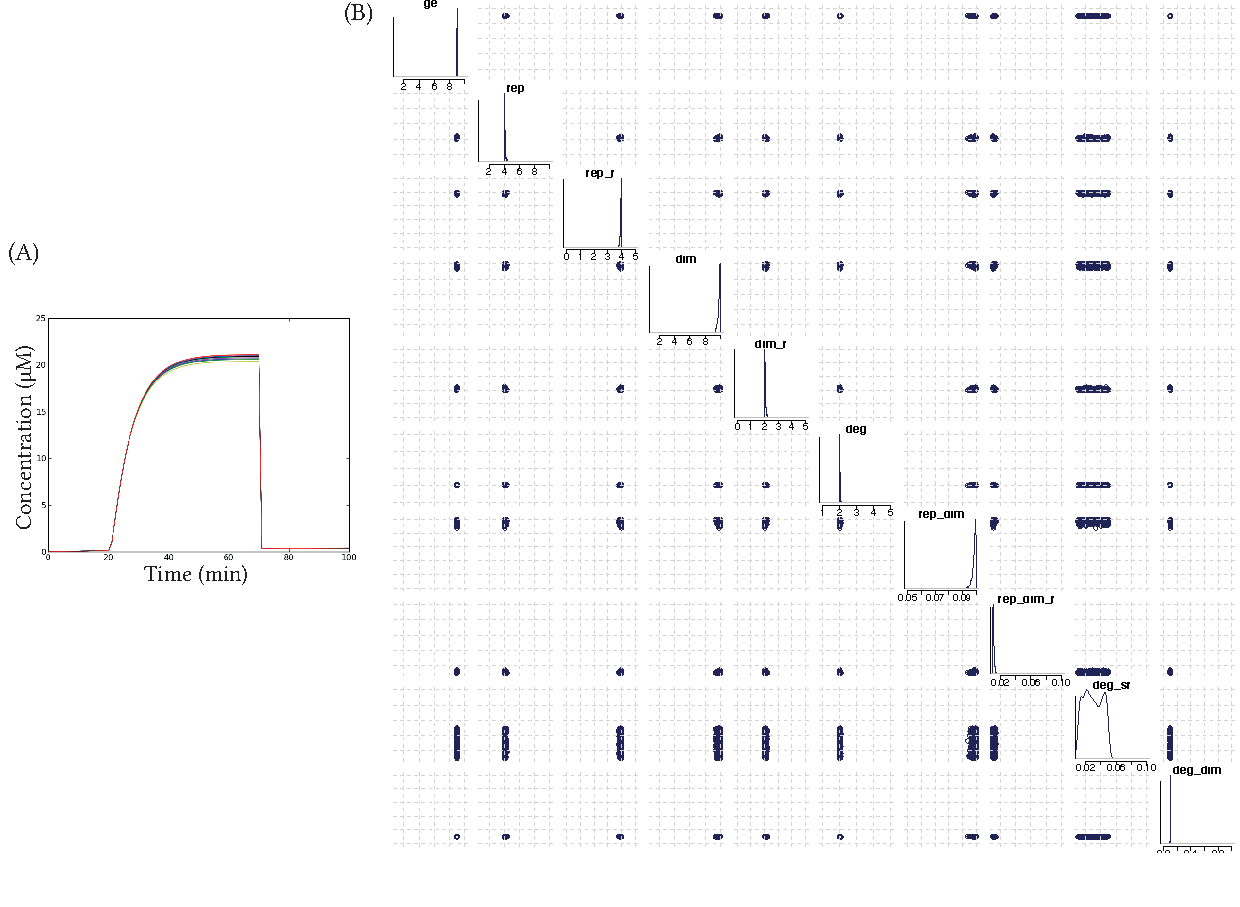
\includegraphics[scale=0.7]{../../chapters/chapterABCSysBio/images/param_inf_res.png}
    \caption{(A) The time series of the final population (for final $\epsilon$ = 2 ) of the standard toggle switch ABC-SMC parameter inference. The stimulus, that represses A2, is added at t=20 and the repressor, that represses B2 is added at t=70. (B) The posterior distribution of the toggle switch.}
    \label{fig:stand_abc_timeseries}
\end{figure}
\clearpage
    

The standard toggle switch model was shown to successfully behave like a switch within the parameter range used here.  By examining Figure~\ref{fig:stand_abc_timeseries}B, I conclude that for this model to behave like the design principles defined, gene expression (ge) must be high relative to the prior. Repression (rep) and degradation must both be low and the rate of dimerisation (dim) must be high relative to the prior. These specifications will be useful when building such a switch in the lab, as the appropriate components must be tweaked. More generally, it can be seen in Figure~\ref{fig:stand_abc_timeseries}B, that the posterior distribution that can produce such a behaviour is narrow, which means there is a small combination of parameter values that can produce this behaviour. In the next section I will examine wether the addition of feedback loops can increase the volume of the posterior that produces the required behaviour.


\section{Genetic toggle switch model selection}

In this section I examine wether the addition of feedback loops to the toggle switch can increase its robustness to parameter fluctuations. It is well known that additional feedback interactions can increase robustness to  noise. 

\subsection{Models of the genetic toggle switch}
\label{sec:models_bist}

I consider 7 models for their capability to behave like a switch. The simple toggle switch, switches with positive autoregulation in either or both nodes and switches with negative autoregulation in either or both nodes. The models considered are illustrated in Figure~\ref{fig:toggle_switch_designs}. 


In order to use these models for model selection, it must first be determined whether they are capable of behaving like a switch. ABC model selection is used to select models that can produce the same behaviour, over a greater range of parameter values. If a model is not capable of producing the desired behaviour for the prior range, then it will not be used for model selection. In order to study each model I built extensions to the ~\autocite{Gardner:2000vha} toggle switch in order to incorporate positive and negative feedback to the system.  The models for the double autoregulation models are shown below. For the single autoregulation models, the unnecessary autoregulation term is set to 0.

Double positive autoregulation: 
\begin{align}\label{eq:gards_neg}
\frac{du}{dt} &= \frac{a_1}{1+v^{\beta} + k_{u}^{\delta_{u}}} - u \\
\frac{dv}{dt} &= \frac{a_2}{1+u^{\gamma }+ k_{v}^{\delta_{v}}} - v,
\end{align}

Double negative autoregulation: 
\begin{align}\label{eq:gards_pos}
\frac{du}{dt} &= \frac{a_1+ k_{u}^{\delta_{u}}}{1+v^{\beta}} - u \\
\frac{dv}{dt} &= \frac{a_2+ k_{v}^{\delta_{v}}}{1+u^{\gamma }} - v,
\end{align}

where $k$ represents the effective binding of the transcription factor to its own promoter and $\gamma$ represents the polymerisation of the bound transcription factor. 


\begin{figure*}[htbp]
	\begin{center}
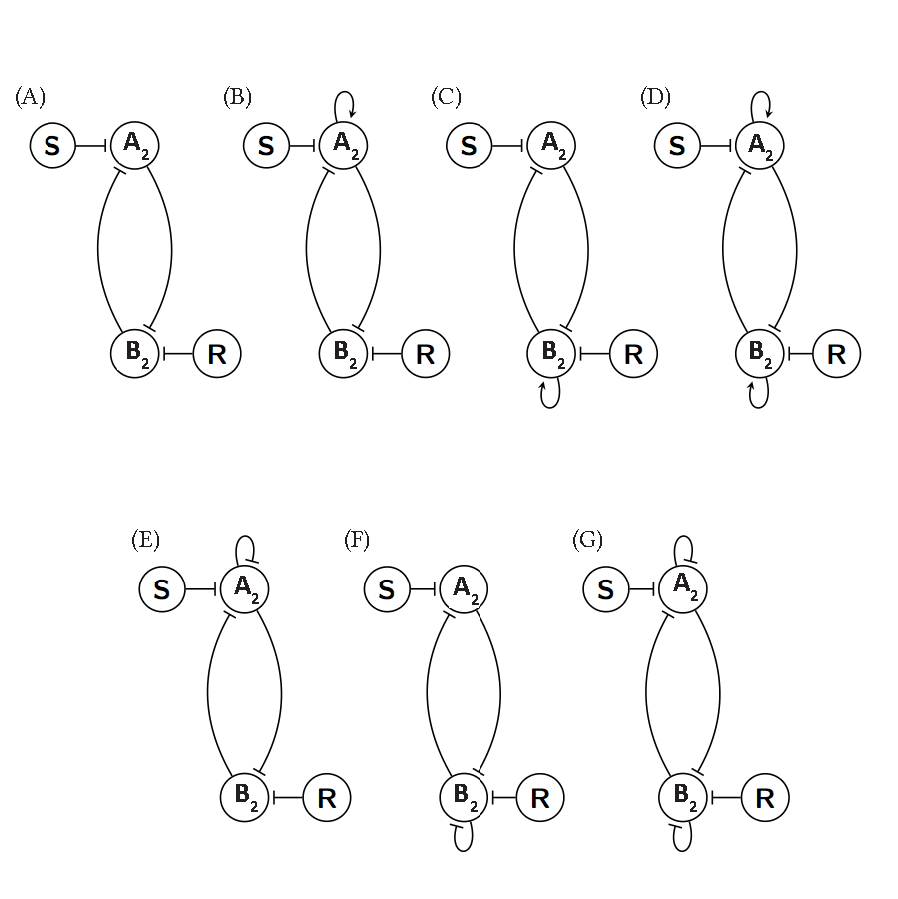
\includegraphics[width=\textwidth]{../../chapters/chapterABCSysBio/images/toggle_switch_designs.png}
\caption[LoF caption]{\label{fig:toggle_switch_designs}: Toggle switch designs considered for model selection}
\end{center}
\end{figure*}
\clearpage


I used the PyDSTool~\autocite{Clewley:2012kj} in order to determine whether each of the 7 switches is capable of bistable behaviour. As shown in Figure~\ref{fig:Gard_pos}, both single and double positive autoregulation is consistent with bistable behaviour. Two stable and one unstable steady state were found for both cases when $k$ = 2 and $\gamma$ = 1. 


\begin{figure*}[htbp]
	\begin{center}
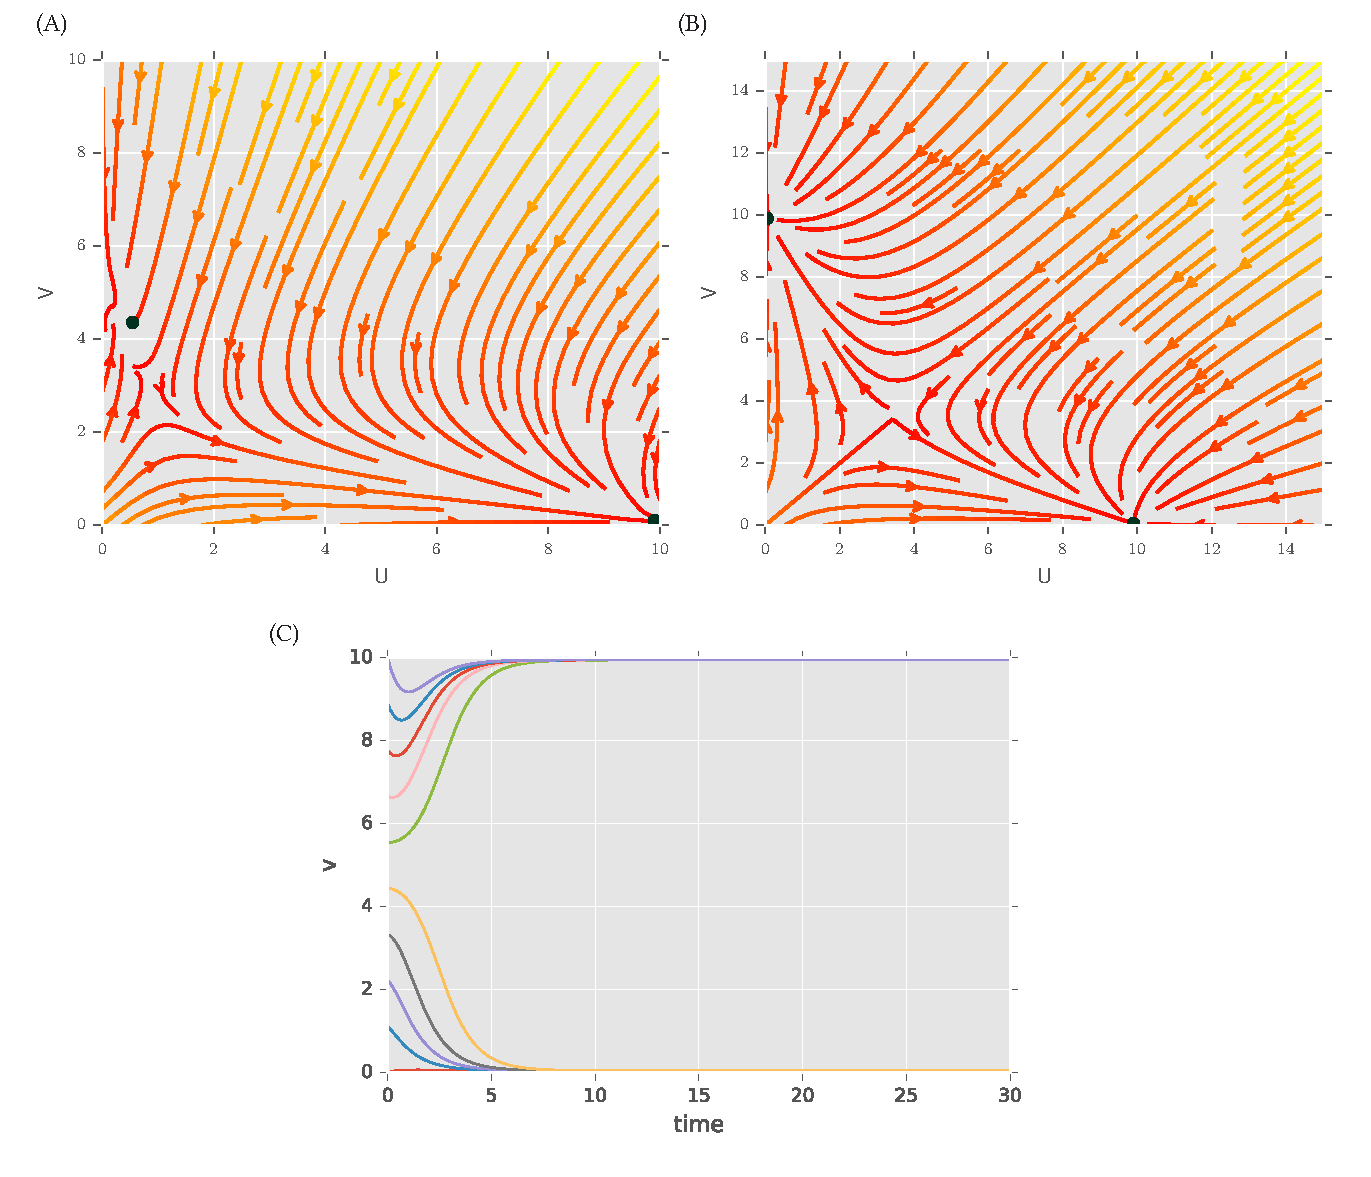
\includegraphics[scale=0.6]{../../chapters/chapterABCSysBio/images/gard_pos.png}
\caption[LoF caption]{\label{fig:Gard_pos}: Both single and positive autoregulation is consistent with bistable behaviour. Two stable and one unstable steady state is found for each model. (A) Single positive autoregulation and (B) double positive autoregulation vector plots.}
\end{center}
\end{figure*}

On the other hand, negative autoregulation was not consistent with bistable behaviour. A bifurcation analysis, when all other parameters are kept constant and only $k$ varied, shows that  even small values of $k$ destroy bistability. This is shown in Figure~\ref{fig:Gard_neg}C. 
\begin{figure*}[htbp]
	\begin{center}
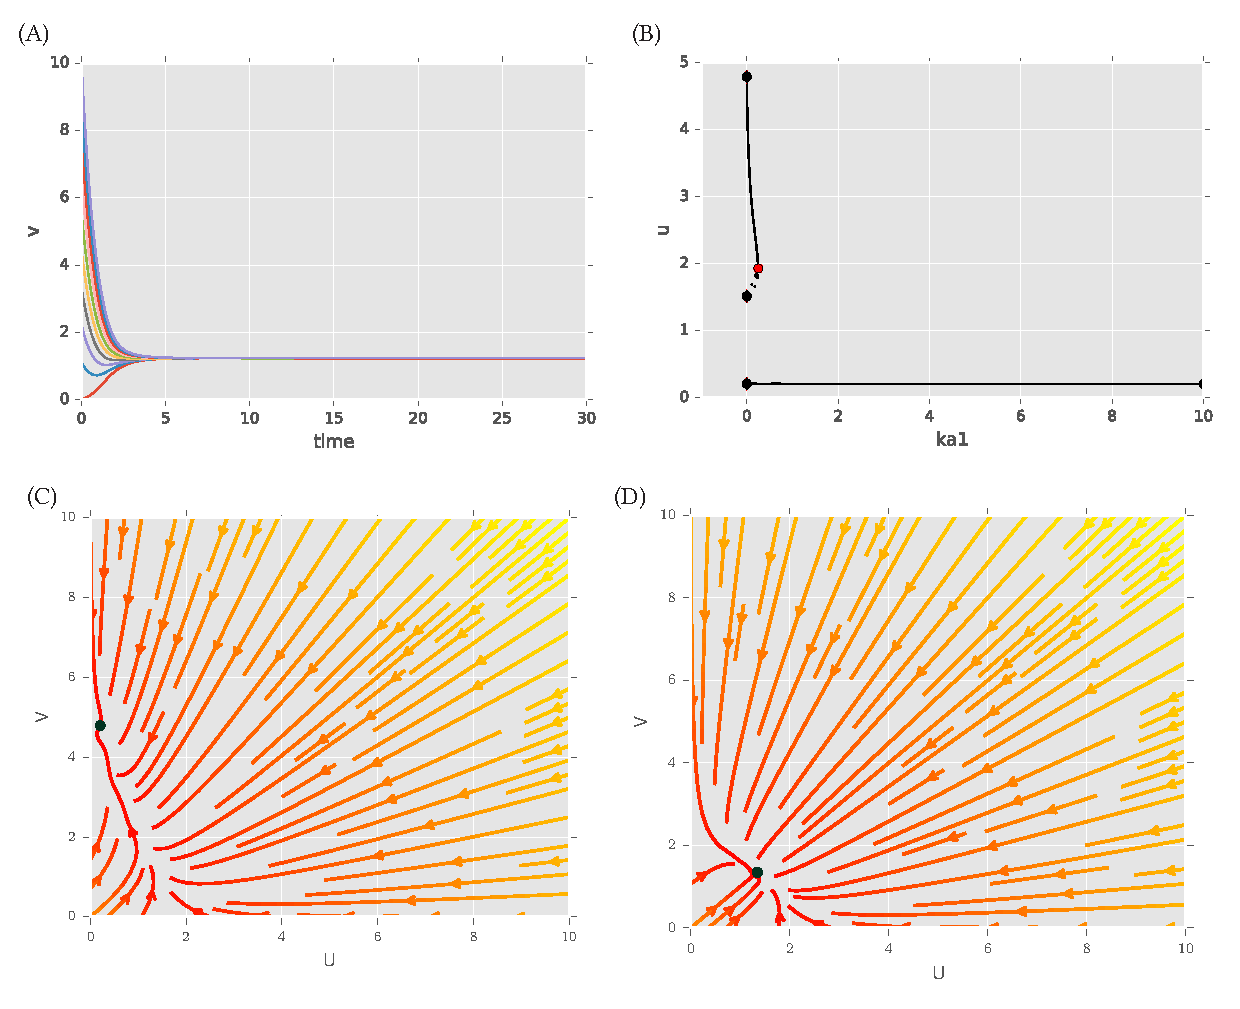
\includegraphics[scale=0.7]{../../chapters/chapterABCSysBio/images/gard_neg.png}
\caption[LoF caption]{\label{fig:Gard_neg}:(A) Timecourse of the single negative autoregulation switch, when $k_u$=2 with varying initial conditions. The system is monostable. (B) One stable and one unstable steady states are found for the single negative autoregulation switch when $k_u$=2 (C) Bifurcation diagram of the single positive autoregulation switch, where all parameters remain constant and only $ku$ varied. (D) The vector plot of the switch with double negative autoregulation. The switch is monostable.}
\end{center}
\end{figure*}




\clearpage




%the rational comparison of models under parameter uncertainty using Bayesian model selection, which automatically accounts for model complexity (number of parameters) and robustness to parameter uncertaint


\subsection{\acrlong{abc} for model selection}

Using the models shown in Section~\ref{sec:models_bist} to exhibit bistability, model selection is carried out. Bayesian model selection is used to directly compare the competing designs using ABC-SysBio~\autocite{Liepe:2010eg}. This method enables the simultaneous inference of the kinetic parameters and the structure of the models in order to select the model producing the same behaviour over a greater parameter range. \acrshort{abc} \acrshort{smc} can be used for model selection by adding the model as a parameter to the selection process. The algorithm samples models as well as parameters at each iteration. When the last \textepsilon{} is reached, the algorithm will have concluded to a posterior distribution of parameters for each model, a subset of the prior distribution that can give the best rise to the data. The model that performs over a greater posterior parameter range is selected as the most robust~\autocite{Toni:2009tr}. The process is outlined in Figure~\ref{fig:abc_model_sel}.
    
\begin{figure*}[htbp]
	\begin{center}
\includegraphics[scale=0.5]{../../chapters/chapterABCSysBio/images/model_selection.png}
\caption[LoF caption]{\label{fig:abc_model_sel}: Model selection}
\end{center}
\end{figure*}
\clearpage


In order to select for the more robust toggle switch, the standard toggle switch will be compared to switches with positive auto-regulation in one or both nodes. The more realistic mass action models were used for model selection, with the addition of two inducers, one turning the switch on by repressing AA and one turning the switch off by repressing BB. The following equations are added to the equations of the simple toggle switch used in Section~\ref{sec:paramscan}. Toggle switches with autoregulation on both nodes have both relevant sets of equations added. 

Positive autoregulation on A:

$$
\begin{array}{cccc} 
    \textrm{A2} + \textrm{gA} \stackrel{\textrm{aut 1}}{\longrightarrow} \textrm{A2gA} \\
    \textrm{A2gA} \stackrel{\textrm{aut 2}}{\longrightarrow} \textrm{A} + \textrm{A2gA}\\
    \textrm{A2gA} \stackrel{\textrm{aut 3}}{\longrightarrow} \textrm{A2}+ \textrm{gA}  \\
\end{array}
$$

Positive autoregulation on B:

$$
\begin{array}{cccc} 
    \textrm{B2} + \textrm{gB} \stackrel{\textrm{aut\_1}}{\longrightarrow} \textrm{B2gB} \\
    \textrm{B2gB} \stackrel{\textrm{aut\_2}}{\longrightarrow} \textrm{B} + \textrm{B2gB}\\
    \textrm{B2gB} \stackrel{\textrm{aut\_3}}{\longrightarrow} \textrm{B2}+ \textrm{gB}  \\
\end{array}
$$

%Negative autoregulation on A:
%
%$$
%\begin{array}{cccc} 
%    \textrm{A2} + \textrm{gA} \stackrel{\textrm{aut\_1}}{\longrightarrow} \textrm{A2gA} \\
%    \textrm{A2gA} \stackrel{\textrm{aut\_2}}{\longrightarrow} \textrm{A2}+ \textrm{gA}  \\
%\end{array}
%$$
%
%Negative autoregulation on B:
%
%$$
%\begin{array}{cccc} 
%    \textrm{B2} + \textrm{gB} \stackrel{\textrm{aut\_1}}{\longrightarrow} \textrm{B2gB} \\
%    \textrm{B2gB} \stackrel{\textrm{aut\_2}}{\longrightarrow} \textrm{B2}+ \textrm{gB}  \\
%\end{array}
%$$

Given the models shown above and the parameter priors used for the standard toggle switch parameter inference, ABC SMC model selection is carried out. The results are shown in Figure~\ref{fig:model_sel_res}. The toggle switch with positive autoregulation on A is found as the most robust model using ABC-SysBio. 



\begin{figure*}[htbp]
	\begin{center}
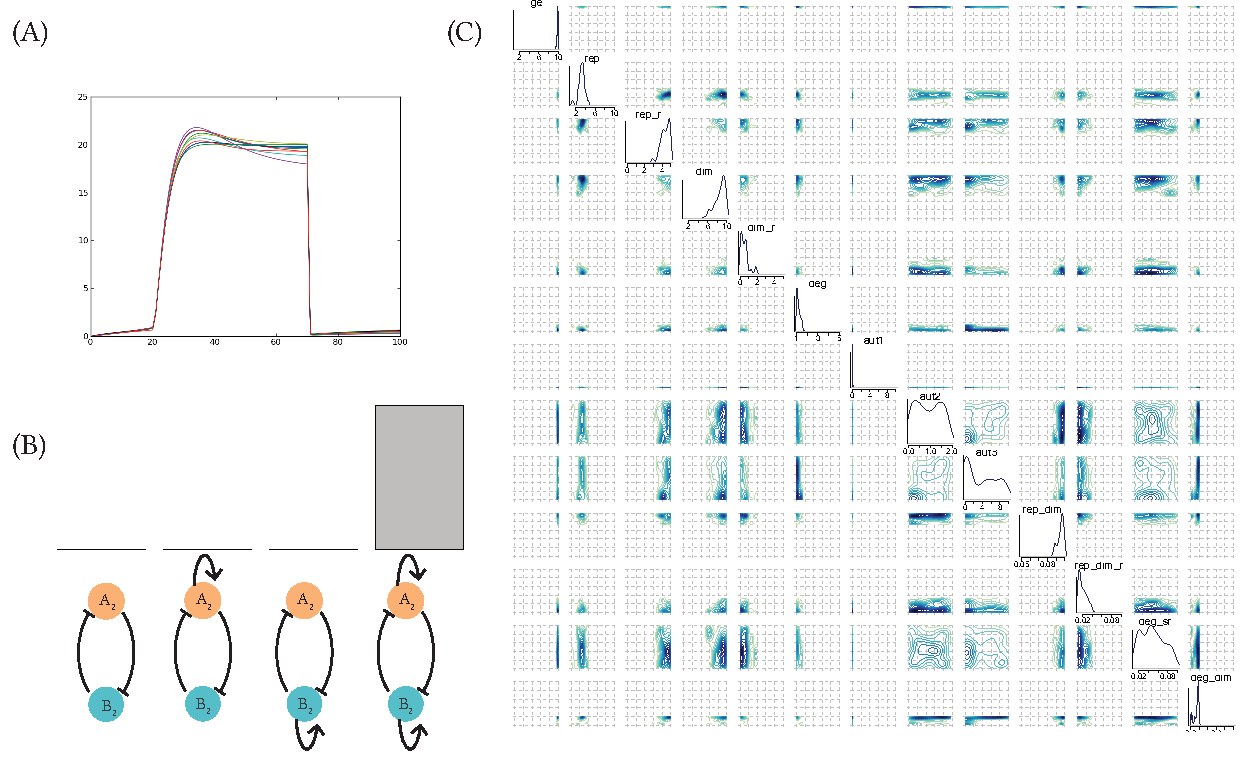
\includegraphics[scale=0.75]{../../chapters/chapterABCSysBio/images/model_sel_res.png}
\caption[LoF caption]{\label{fig:model_sel_res}: (A) The toggle switch models considered. Interactions denoted by a circular arrow head can be positive of zero. (B) The toggle switch with positive autoregulation on A was found to be the most robust to parameter fluctuations. (C) The posterior distribution of the toggle switch with positive autoregulation on A.}
\end{center}
\end{figure*}
\clearpage

\section{Discussion}

Constraints are too many for accurate analysis (the behaviour is too specific).
%From parameter scan
Further analysis is thus needed to determine what these combinations are. A sensitivity analysis of the model will be carried out in order to determine which parameters affect bistability and to which parameters is the system robust. The parameter scan will also be incorporated into the ABC SMC methodology, in order to identify the parameter values required for bistability more efficiently.             

In this work it was shown that a range of stability profiles are achievable by the standard toggle switch. The patterns of the parameter values required for each are beginning to emerge. Further work is required in order to get a definitive answer for the stability characteristics of the toggle switch given this modelling approach.


\clearpage
\section{Summary}

In this chapter I studied the~\textcite{Gardner:2000vha} toggle switch and showed that it is bistable. I further studied the genetic toggle switch by using mass action to represent the model, and removing the \acrshort{qssa} approximation from the models. I identified the parameter ranges that produce a bistable behaviour and could be used as prior distributions for parameter inference. Further, I studied the effect of adding feedback loops has on the robustness of the genetic toggle switch. In the next chapter I address these shortcomings by developing a new algorithm, StabiliyFinder. 





%% StabilityFinder ----------------------------------%%
\mainmatter*
 
\chapter{Dynamics of multi-stable switches}
\label{ch:SF}
\section{Introduction}

In this chapter, I aim to uncover the underlying principles that govern the stability of a given switch. To do this, I developed an algorithm, called StabilityFinder, that can identify the parameter value ranges that can produce the desired stability in a given model. I use this algorithm to examine a variety of switch architectures using different modelling abstractions.

Structurally, this chapter is organised as follows: In the first section I examine the current understanding of the stability landscape of the genetic toggle switch. Then, I discuss the development of StabilityFinder, justify the choices made and the drawbacks of this method. In the sections following I apply StabilityFinder to a variety of models and finally I discuss the implications these findings have to the overall understanding of the toggle switch stability. 

\section{Contributions to this Chapter}
The phase plots of the Lu switch and the characterization of their steady states shown in Figure~\ref{fig:lu_bifurc} was carried out by Mae Woods, PhD.

\section{Motivation}
%A circuit must be robust to a fluctuating cellular environment and its response and sensitivity must be able to be fine tuned in order to orchestrate a network of circuits that function together. A robust circuit can tolerate the compound stochasticity that a chain of circuits brings, and fine tuning of its response and sensitivity enables the researcher to make it sensitive to an upstream signal as well as influence a downstream subsystem. %

Synthetic biology puts an emphasis on creating modular, standardized parts that can be used to create larger systems~\autocite{Agapakis:2009bt}. When faced with the creation of a new model design, the researcher can select the appropriate parts from the BioBrick registry~\autocite{Muller:2011bp} and combine them to create the system of choice. Synthetic circuit design presents a challenge as the collection of assembled parts have to work together to create the target behaviour~\autocite{Nielsen:2013hs}. Parts can be fine tuned by developing component libraries~\autocite{Lu:2009ez}, but this will be of little use if the required parameter ranges for parts to make a functional system are unknown, and will only perpetuate the cycles of trial-and-error. A computational method to find the range of parameter values that will produce the behaviour of choice is crucial to the design process by enabling the informed selection of appropriate parts from the libraries. For example, if it is known that gene expression must be low for a given stability, one can select a weak promoter or a low copy plasmid for the desired construct. 

Both analytical and computational approaches have been deployed for the study of the toggle switch. Analytical approaches are limited to simpler models and thus require a number of assumptions to be made. The system under consideration has to be reduced to very few equations and parameters in order to make the system solvable. This requires assumptions to be made about the system that cannot always be justified, such as the~\acrfull{qssa}. The \acrshort{qssa} assumes that the binding/unbinding processes are much faster than any other process~\autocite{Loinger:2007vma}, thus the bound intermediate is assumed to always be in steady state. The \acrshort{qssa} assumption is met \textit{in vitro} but often does not hold \textit{in vivo} and its misuse can lead to large errors and incorrectly estimated parameters~\autocite{Pedersen:2007ke}. Moreover, it is generally not possible to solve even simple stochastic models analytically, and these methods are restricted to deterministic models. The computational and graph-theoretic approaches developed for the study of multistationarity generally focus on deciding on whether a given system is incapable of producing multiple steady states ~\autocite{Conradi:2007jo, Banaji:2010fh,Feliu:2013dz}. For example,~\textcite{Feliu:2013dz} developed an approach using chemical reaction theory and generalised mass action modelling \autocite{Feliu:2013dz}. No approach exists that can handle both deterministic and stochastic systems in an integrated manner.

For this purpose, I developed a computational framework based on sequential Monte Carlo that takes a model and determines whether it is capable of producing a given number of steady states and the parameter space that gives rise to the behaviour. Uniquely, this can be done for both deterministic and stochastic models, and also complex models with many parameters, thus removing the need for simplifying assumptions. This framework can be used for comparing the conclusions drawn by various modelling approaches and thus provides a way to investigate appropriate abstractions. I have made this framework into a python package, called StabilityFinder. 

I use this methodology to investigate genetic toggle switches and uncover the design principles behind making a bistable switch, as well as those necessary to make a tristable and a quadristable switch (4 steady states). The number of stable steady states will be referred to as the desired stability of the model in this thesis. I also demonstrate the ability of StabilityFinder to examine more complex systems and examine the design principles of a three gene switch. The examples I used demonstrate that StabilityFinder will be a valuable tool in the future design and construction of novel gene networks. 




%\section{Parameter scan}
%\subsection{Background}
%
%    
%\subsection{Methods}
%
%\par
%A scan of the parameter values and initial species concentrations of the general toggle switch (shown in Figure~\ref{fig:Toggle switch example}) was performed in this work. This illustrated the presence of tristable, bistable and monostable systems given a different set of parameter values. In addition, the scan was carried out to identify a set of parameter values that leads to a bistable system with maximum distance between the two steady states. This system is able to produce high amounts of the response protein when switched on. A symmetric model, where the parameters for equivalent reactions were set to be the same, was used for simplicity. The algorithm of the scans is outlined below:
%
%\begin{algorithm}[H]
%	\label{alg:param_scan}
%  \caption{Parameter scan}
% \begin{algorithmic}[1]
%    \Statex
%	\State Sample parameters from $U(0, 10)$
%	\ForAll{Sample}
%    	\State Sample initial conditions via Latin Hypercube sampling~\autocite{Mckay:2000lhs}
%    	\ForAll{Samples}
%    		\State Simulate model
%    		\State Solve to steady state
%    	\EndFor
%    \EndFor
%  \end{algorithmic}
%\end{algorithm}
%
%%\begin{itemize}
%%\item Select multiple sets of parameter values from a random uniform distribution between 0 and 10.
%%\item For each set of parameter values:
%%    \begin{itemize}
%%    \item Select multiple sets of initial conditions for the two dimers via latin hypercube sampling:
%%    The space from which the sampling will take place, here between 0 and 10 for both species, is divided equally into 100 smaller subspaces and one value is selected from each subspace~\autocite{Mckay:2000lhs}. Therefore it is ensured the whole space is sampled from. 
%%    \item For each set of initial conditions:
%%        \begin{enumerate}
%%        \item Integrate ODEs of the model
%%        \item Solve system to steady state
%%        \end{enumerate}
%%    \end{itemize}
%%\end{itemize}
%
%
%
%One dimer was plotted against the other for all initial conditions of each parameter set. An example for each of the three types of stabilities found during the scan are shown in Figure~\ref{fig:stab exampl}. The parameter sets that resulted in bistability are shown in Table ~\ref{tab: scan params}. 
%
%\subsection{Results}
%\begin{figure}[h!]
%\centering
%\includegraphics[scale=0.9]{../../chapters/chapterStabilityFinder/images/switch_stbility_examples.pdf}
%\captionof{figure}{An example for each type of switch found during the parameter scan. Each graph represents the steady state values of one dimer plotted against the other, from one parameter set and 100 initial conditions.}
%    \label{fig:stab exampl}
%\end{figure}
%
%In order to determine which areas in the parameter space give rise to the different kinds of stability, a histogram of the frequency of each parameter value found in monostable, bistable and tristable systems was plotted and shown in Figure~\ref{fig:scan ode param hist}.
%
%
%\begin{figure}
%\centering
%\begin{minipage}[c]{1\textwidth}
%\centering
%    \includegraphics[width=1.05\textwidth]{../../chapters/chapterStabilityFinder/images/param_stability_hist.pdf}
%    \caption{The distribution of parameter values that resulted in monostable, bistable and tristable switches in the parameter scan. Each graph represents the distribution of the values of one parameter. }
%    \label{fig:scan ode param hist}
%\end{minipage}
%\end{figure}
%
%
%
%\begin{table}[h!]
%\centering
%\caption {The parameter values obtained from the parameter scan that resulted in bistability. Each row corresponds to a set of parameter values.} \label{tab: scan params}
%\begin{tabular}{ccccccc}
%\toprule
% \textbf{ge}     & \textbf{rep}    & \textbf{rep r}     & \textbf{dim}    & \textbf{dim r}     & \textbf{deg      }\\
% \midrule
%6.95   & 9.53    & 1.890     & 6.43   & 7.06      & 2.91   \\
%4.82   & 4.37    & 0.595     & 9.45   & 2.07      & 3.72   \\
%8.44   & 6.53    & 0.818     & 8.15   & 3.59      & 9.99   \\ 
%6.46   & 7.92    & 2.650     & 3.07   & 8.01      & 1.91   \\
%8.15   & 9.42    & 1.44      & 6.13   & 5.45      & 4.84     \\
%8.89   & 8.98    & 5.39      & 3.56   & 7.39      & 2.24     \\
%8.01   & 9.95    & 5.69      & 5.95   & 4.01      & 1.90     \\
%6.28   & 4.88    & 2.11      & 4.96   & 2.44      & 4.24     \\
%9.48   & 9.40    & 3.69      & 2.16   & 3.95      & 2.08     \\
%7.72   & 6.19    & 2.31      & 5.97   & 1.58      & 5.40     \\
%3.60   & 3.80    & 0.43      & 8.90   & 4.66      & 2.24     \\
%8.23   & 4.31    & 2.07      & 7.94   & 3.52      & 6.32     \\
%9.36   & 7.33    & 7.47      & 8.19   & 9.87      & 2.99   \\
%8.16   & 2.08    & 1.36      & 3.29   & 8.27      & 1.62   \\
%8.52   & 8.09    & 4.41      & 4.25   & 1.23      & 6.48   \\
%8.15   & 4.42    & 1.05      & 5.44   & 9.57      & 2.16   \\
%\bottomrule
%\end{tabular}
%\end{table}   
%   
%\clearpage
%\subsection{Discussion}
%\par
%   The parameter scan was successfully completed in the deterministic case and some of the results shown in Figure \ref{fig:stab exampl}. Different parameter sets resulted in different stability of the toggle switch.   
%     
%\par
%   There were a total of 217 monostable, 16 bistable and 6 tristable switches out of 400 sampled parameter sets. The remaining samples did not reach steady state. This shows that different parameter values have a great effect on the stability profile of the switch. Note the symmetry of the steady states of each bistable switch is due to the use of a symmetric model. 
% 
%\par 
%    Some interesting results arise from the histograms in Figure ~\ref{fig:scan ode param hist}. It can be seen that the parameter for gene expression (ge) tends to be relatively high when bistability arises whereas the parameter for the reverse reaction of repression (rep r) tends to be low. Degradation (deg) also tends to be low. It must also be noted that the parameter values that give rise to monostable systems are generally evenly distributed for all parameters, suggesting that monostable systems arise from the whole range of values sampled. This can further indicate that the right combination of more than one parameter values is necessary for bistability. Further analysis is thus needed to determine what these combinations are. A sensitivity analysis of the model will be carried out in order to determine which parameters affect bistability and to which parameters is the system robust. The parameter scan will also be incorporated into the ABC SMC methodology, in order to identify the parameter values required for bistability more efficiently.             
%
%\par
%    In this work it was shown that a range of stability profiles are achievable by the standard toggle switch. The patterns of the parameter values required for each are beginning to emerge. Further work is required in order to get a definitive answer for the stability characteristics of the toggle switch given this modelling approach.
%
%\section{Bayesian approach to model stability}
\section{StabilityFinder algorithm}

To investigate the multistable behaviour of systems, I had to make a number of extensions to existing approaches. Firstly, a wide range of initial condition samples are required in order to determine the stability of a system. For a given set of parameter values, sample points are taken across initial conditions using latin hypercube sampling~\autocite{MCKAY:2000vt}, and the ensemble system simulated in time until steady state. As a distance function I use the desired stability of the simulated model. An overview of the algorithm is given in Section~\ref{sec:Alg_overview}. %Then each module in the algorithm is described in Sections~\ref{sec:part_samp}-\ref{sec:mod_check}.


\subsection{Algorithm overview}
\label{sec:Alg_overview}
The StabilityFinder algorithm is summarised below. StabilityFinder is available as a Python package, and can be downloaded from \url{https://github.com/ucl-cssb/StabilityFinder.git}. 

\begin{figure*}[h]
\begin{center}
\includegraphics[scale=0.9]{../../chapters/chapterStabilityFinder/images/SF_algo_overv.png}
\caption[StabilityFinder algorithm overview]{\label{fig:fig1}Using sequential Monte Carlo to examine system stability. The algorithm takes as input a model (A) and evolves it (B) to the stability of choice via (C) intermediate populations. In this example model shown in (A), There are two species and two parameters. For the model to be bistable, the phase plot of the two species of interest must have two distinct densities, as shown in (D). The parameter space of the model is searched through our algorithm until the resulting simulations give rise to bistability. The parameter values for the model that demonstrated the desired behaviour are given as an output (D). The output consists of the accepted values for each parameter, as well as each density plotted against the other. This allows us to uncover correlations between parameter values. This algorithm is available as a python package, called StabilityFinder. The overview of the algorithm is shown in (E).}
\end{center}
\end{figure*}
\clearpage

The user provides an SBML model file~\autocite{Finney:2003vk, Hucka:2004wh} and an input file that contains all the necessary information to run the algorithm, including the desired stability and the final tolerance, ε, for the distance from the desired behaviour necessary for the algorithm to terminate. The flow of execution is illustrated in Figure~\ref{fig:fig1}E. Since the algorithm is computationally intensive, all deterministic and stochastic simulations are performed using algorithms implemented on \acrfull{gpu}s, which are used for mutli-threaded computation~\autocite{Kirk:2010we}.


%The user provides an SBML model file and an input file that contains all the necessary information to run the algorithm, including the desired stability and the final tolerance \textepsilon, for the distance from the desired behaviour necessary for the algorithm to terminate. The flow of execution is illustrated in Figure~\ref{fig:fig1}E. Since the algorithm is computationally intensive, all deterministic and stochastic simulations are parallelised and performed using algorithms implemented on \acrfull{gpu}s. 

%\begin{figure*}[h]
%\begin{center}
%\includegraphics[scale=0.5]{../../chapters/chapterStabilityFinder/images/process_overv.png}
%\caption[LoF caption]{q}
%\end{center}
%\end{figure*}
%\clearpage

%\subsection{Particle sampling}
%\label{sec:part_samp}
%For the first population, particles are sampled from the priors. Random samples are taken from the distribution specified by the user for each parameter. 
%
%For subsequent populations particles are sampled from the previous population. The weight of each particle in the previous population dictates the probability of it being sampled. The number of samples to be drawn is specified by the user in the input file.  
%
%\subsection{Perturbation}
%\label{sec:pertub}
%Each sampled particle is perturbed by a kernel defined by the distribution of the previous population, as developed by~\textcite{Toni:2009tr}. 
%
%\begin{align}
%K_p(\theta|\theta* ) =& \theta* + U(+s_p, -s_p)\text{, where:} \\
%s_p =& \frac{1}{2} \big (max(\theta_{p-1}) - min(\theta_{p-1}) \big )
%\end{align}
%
%If the \texttheta* falls out of the limits of the priors then the perturbation is rejected and repeated until an acceptable \texttheta* is obtained. This method is successful in perturbing the particles by a small amount in order to explore the parameter space, but can be slow to complete. 

\subsection{Initial condition sampling}
\label{sec:init_cond_samp}
In StabilityFinder, latin hypercube sampling is used to sample initial conditions~\autocite{MCKAY:2000vt}. This is used to ensure that the whole space is sampled uniformly. Latin hypercube sampling is done in two dimensions in StabilityFinder. This is the same algorithm used for initial condition sampling in Chapter~\ref{ch:abcsysbio}, and the reader is referred to Section~\ref{sec:paramscan} for a description of this algorithm. StabilityFinder could easily be implemented to be used for a larger number of species, but here it has only been used for stability analyses concerning two species. Stability landscapes involving more that two species are beyond the scope of this thesis. %The uniform priors of the two species in consideration represent a rectangle space, which is subdivided into equal parts. Then a random sample is drawn from each sub-part. This ensures the whole space is evenly sampled. 

%\begin{figure*}[htbp]
%\begin{center}
%\includegraphics[scale=0.5]{../../chapters/chapterStabilityFinder/images/LHS.png}
%\caption[LoF caption]{\label{fig:lhs}Latin hypercube sampling ensures that the whole space is sampled evenly. For the two species concerned, A and B, we assume uniform distributions, shown in grey. The joint space of the two distributions is divided into smaller equal parts and a random sample is drawn from within each subspace.  }
%\end{center}
%\end{figure*}


\clearpage

%\subsection{Particle simulation}
%\label{sec:sim}
%Each particle is simulated using cuda-sim~\autocite{Zhou:2011hp}. The model is provided by the user in SBML format and is converted into CUDA\textsuperscript{\textregistered} code by cuda-sim. The model in CUDA\textsuperscript{\textregistered} code format can then be run on NVIDIA\textsuperscript{\textregistered}. CUDA\textsuperscript{\textregistered}. \acrshort{gpu}s. This allows the user to take advantage of the speed of parallelised simulations without any CUDA\textsuperscript{\textregistered} knowledge. 
%
 
\subsection{Clustering methods}
\label{Clustering methods}

Whether the model was simulated using \acrshort{ode}s or the Gillespie algorithm~\autocite{Gillespie:1977ww} dictated the method of clustering that I used. For the deterministic models I used an algorithm I developed, that will be referred to as the delta clustering algorithm in this thesis. This algorithm consists of defining the number of clusters by counting a new cluster every time a data point is more than a distance δ away from any existing clusters. The benefits of the delta clustering algorithm are that it is fast and can be used on deterministic solutions, where steady state values tend to be identical if all the particles have reached steady state.

Steady states of stochastic models are clustered using the K-means clustering~\autocite{Lloyd:1982wn} and the number of clusters determined using the Gap statistic~\autocite{Tibshirani:2001vo}. This method is more suited to stochastic solutions, where the delta clustering method would fail as the steady state solutions tend to be more widely dispersed than in the deterministic case. The detailed algorithms used are shown in Appendix~\ref{ap:Alg}. 

The method used for clustering can be altered by the user if he/she wants to add their own preferred clustering algorithm that might be more appropriate for their specific purposes. For the models I used here, the above methods were successful in clustering the steady state solutions. 

\subsection{Distance function}
\label{sec:dist}
 The distance function is used to compare the desired behaviour to the behaviour observed in each particle~\autocite{Toni:2009tr}. In StabilityFinder the distance function consists of three distances. The first one is the difference between the number of desired clusters and the number of clusters observed in the phase plot. For this distance metric the number of clusters in the phase plot must be calculated. The clustering methods used are outlined in Section~\ref{Clustering methods}.
 
 The other two distance metrics used in StabilityFinder are the variance within each cluster and the overall (between cluster) variance. The within cluster variance ensures that the clusters are tight, and the between cluster variance is used to ensure the clusters are far apart from each other. In the context of this thesis, the ideal behaviour of a system is tight, widely separated clusters. This means that the genetic system has distinct steady states, and the difference in the protein levels between each steady state is observable.

\begin{align}
	d_1 &= C = M_c \label{eq:dist1}\\
	d_2 &= V_{tot} = \frac{1}{n} \sum_{i=1}^{n}(x_i- \mu)	\label{eq:dist1}\\
	d_3 &= V_{cl} =  \underset{m_c = 1}{\overset{Mc}{\mathrm{median}}} \{ \frac{1}{n_{m_c}} \sum_{c=1}^{n_{m_c}}(x_c- \mu_c)\} \label{eq:dist3},
\end{align}
where $n$ denotes the total number simulations per particle, $x$ refers to each  simulation steady state of a given particle and μ the mean value of all the simulations steady states in each particle. $M_c$ denotes the total number of clusters per particle and $m_c$ refers to each cluster. $x_c$ and $\mu_c$ represent the simulation steady state of a given particle in the current cluster and the mean of the current cluster respectively.   


%\subsection{Particle rejection}
%\label{sec:rej}

Once the distance from the desired behaviour has been calculated, the algorithm rejects any particles whose distance is farther than the current ε. The distances taken into account are the number of clusters ($C$), the total variance (V\textsubscript{tot}) and the within cluster variance (V\textsubscript{cl}) as outlined in Equations~\ref{eq:dist1}-\ref{eq:dist3}. In addition to these distances I have included another two checks for the particles. Firstly, StabilityFinder checks if the simulation of a particle has reached steady state. If the standard deviation of the last ten time points in the simulation (denoted as $SS_{ss}$) is larger than a user-specified value, then the particle is rejected. This is to ensure that only particles that have reached steady state are considered. Secondly, there is a check for the minimum level of the steady states (denoted as $SS_{l}$). This is to allow the user to select for steady states whose protein levels are above a certain threshold. This has to be added as an additional check as the steady state levels must be experimentally observable if they are to be used to design new systems. Two steady state levels of very low levels would be biologically indistinguishable and thus meaningless in an experimental setup. This check is optional to the user, and can be set to zero if not desired. In summary, a particle must satisfy all of the criteria given below in order to be accepted:

\begin{align*}
	M_c &\leq ε_{M_c} \\
	V_{tot} &\leq ε_{V_{tot}}\\
	V_{cl} &\leq ε_{V_{cl}}\\
	SS_{ss} &\leq ε_{SS_{ss}}\\
	SS_{l} &\leq ε_{SS_{l}}
\end{align*}



%\begin{enumerate}
%	\item Cluster distance \textgreater \textepsilon\textsubscript{c}
%	\item V\textsubscript{bc} distance \textgreater \textepsilon \textsubscript{Vbc}
%	\item V\textsubscript{wc} distance \textgreater \textepsilon \textsubscript{Vwc}
%	\item SS\textsubscript{v} \textgreater \textepsilon \textsubscript{ssv}
%	\item SS\textsubscript{l}  \textgreater \textepsilon \textsubscript{ssl}
%\end{enumerate}
% 

%\subsection{Weight calculation}
%\label{sec:weight}
%For the first population the weights are all given a value of 1, and then normalised over the number of particles. For subsequent populations the weights of the particles are calculated by considering the weights of the previous population~\autocite{Toni:2009tr}. 
%
%\begin{align}
%w_{t}^{(i)} = \frac{P(\theta_{t}^{(i)})}{\sum_{j=1}^N w_{t-1}^{(j)} K_{t}(\theta_{t-1}^{(j)}, \theta_{t}^{(i)})} \text{ for n $\textgreater$  0}
%\end{align}
%	
%The weights are then normalised over the total number of particles. 
%    

\subsection{Model checking}
\label{sec:mod_check}
A problem that can arise by using this method with stochastic simulations is that the behaviour observed may not be the true behaviour but it might be a result of noise. We need to ensure that the resulting behaviour is reproducible. Therefore, I added model checking to the algorithm. Model checking consists of resampling from the posterior distribution and simulating each sample. If the resulting behaviour is the same as what we expected we can be confident that it is the true behaviour of the system and not a result of noise. 
\begin{algorithm}[htbp]

\caption{ StabilityFinder algorithm}
\label{alg:StabilityFinder}
 \begin{algorithmic}[1]
    \Statex
	\State Initialise $t=0$, 
	\State $i=0$ 
	\If{t $= 0$}
		\State Sample particle from prior, $\theta^{**} \sim \pi(\theta)$
	\Else
		\State Sample $\theta^*$ from the previous population $\{ \theta_{t-1}^{i} \}$ with weights $w_{t-1}$.
		\State Perturb the particle, $\theta^{**} \sim K_t(\theta|\theta^{*})$ where $K_t$ is the perturbation kernel.
	\EndIf
	
	\State Sample $k$ initial conditions $\{ x_0^k \}$ via latin hypercube sampling.
	\State Simulate $k$ datasets to steady state, $\{ x^{*k} \}$, from the the model, $ x^{*} \sim f(x|\theta, x_0)$
    	\State Apply clustering in phase space on $\{ x^{*k} \}$
    	\State Calculate the distance $ d = \rho( \{ x^{*k} \},y)$. 
    	\If{$d \leq \epsilon_t$}
	\State $\theta^{i}_{t} = \theta^{**}$.  $i = i + 1$
	\If{ $i \le N$ } 
		GoTo step 3
	\Else
	\State Calculate weight for each accepted $\theta^{i}_t$
	\State $w_{t}^{(i)} = \begin{cases} 1, & \mbox{if } t = 1 \\\frac{\pi(\theta_{t}^{(i)})}{\sum_{j=1}^N w_{t-1}^{(j)} K_{t}(\theta_{t-1}^{(j)}, \theta_{t}^{(i)})}, & \mbox{if } p \geq  1. \end{cases}$
	\State Normalise weights
	\State $t = t + 1$. 
	\If{ $t \le N_t$} 
	\State GoTo step 3 
	\EndIf
	\EndIf
	\EndIf	
\end{algorithmic} 
\end{algorithm}

\clearpage

\section{Calculating robustness}
\label{sec:cal_rob}
Unlike~\textcite{Toni:2009tr}, StabilityFinder does not have model selection integrated into the method. This is because the purpose of StabilityFinder is not necessarily to compare models for robustness but to elucidate the stability a given model is capable of. Nevertheless, robustness analysis is an outcome that Bayesian methods are well suited for. Therefore, here I discuss another algorithm I developed in order to extract robustness information from the results of StabilityFinder and apply model selection.  

As discussed in Section~\ref{sec:rob_back}, two models $M_a$ and $M_b$ can be compared for their robustness using the Bayes factor, defined as follows:

\begin{align}
 B_{ab} &= \frac{p(D|M_a)}{p(D|M_b)}, \label{eq:final_bayes1}
\end{align}	

\noindent which represents the fraction of the evidence supported by model $a$ over the evidence supported by model $b$. This can be interpreted as the ratio of the fraction of the volume of the functional region to the volume of its prior of model $a$ and model $b$:

\begin{align}
 B_{ab} &= \frac{|F_a|}{|P_a|} / \frac{|F_b|}{|P_b|}, \label{eq:final_bayes2}
\end{align}	

\noindent where $|F|$ is the volume of the functional region of model and $|P|$ the volume of the prior. Equation~\ref{eq:final_bayes2} represents the ratio of the robustness measure of each model which in turn is defined as the ratio between the volume of functional region $F$ and the volume of the prior $P$. The reader is referred to Section~\ref{sec:rob_back} for a further discussion.

In order to calculate the Bayes factor we must first be able to approximate the volume of the viable parameter space. The viable parameter space is the space that approximates the posterior distribution that can give rise to the desired behaviour. I tested two methods of approximating the volume of the viable space, which are outlined in Algorithm~\ref{alg:robustness}. The first method is based on the method used by~\autocite{Hafner:2009ct}, where the volume of the cuboid containing all the viable space is calculated. I modified this part of their method by only including the area of the viable space where the majority of the last population lies. Therefore only the 1\textsuperscript{st} and 99\textsuperscript{th} percentile of the viable space are taken into account. This is necessary in order to exclude outliers in the distribution that would skew the volume calculation significantly. Each parameter represents a side in the cuboid and since the volume of a cuboid is equal to the product of its sides, the volume of the viable space is equal to the product of the ranges of all the parameters. This cuboid method will be prone to overestimating robustness especially in cases of correlation between parameters. This caveat could be alleviated if a \acrfull{pca}~\autocite{Fukunaga:2013wt} is done on the data before the cuboid is calculated~\autocite{Hafner:2009ct}. This would align the axes of the cuboid to the major axes of the distribution. This would still be a crude estimation of the volume, since if the posterior distribution is assumed to be normally distributed the volume would still be overestimated. 

Thus I used a second method, where the volume of the viable space was represented by a hyper-ellipsoid, an ellipse in higher dimensions. This method should not be as prone to overestimation of robustness as the cuboid method as an ellipsoid can take correlation into account. For this method the distribution of the viable space is assumed to be normal. The method calculates the covariance matrix of the distribution, whose volume is given by Equation~\ref{eq:el_vol}. Just as in the cuboid method, the 1\textsuperscript{st} and 99\textsuperscript{th} percentile of the data is ignored. 

\begin{align}
	V & = \frac{2\pi^{\frac{k}{2}}}{k\Gamma(\frac{k}{2})} \Big[ \chi _{k}^{2}(\alpha) \Big]^{\frac{k}{2}} |\Sigma|^\frac{1}{2}, \label{eq:el_vol}
\end{align}
\noindent where k is the number of dimensions, \textGamma{} is the Gamma function, \textalpha{} is the confidence interval required and |$\Sigma$| is the determinant of the covariance matrix. %In this case p = 3, \textalpha{} = 0.025

To validate these methods I compare them to ABC-SysBio model selection~\autocite{Liepe:2014iw}. ABC-SysBio has been used extensively for model selection~\autocite{Toni:2009tr, Toni:2011jy, Barnes:2011hh} and is thus used as a benchmark to the algorithm used here. I use two examples used in the ABC-SysBio package~\autocite{Toni:2009tr} as well as in~\textcite{Toni:2010}. 
%There is good agreement between the three methods as can be seen in Figures~\ref{fig:rob_sysbio1} and \ref{fig:rob_sysbio4}.


\begin{algorithm}[htbp]
\caption{Approximating robustness}
\label{alg:robustness}

 \begin{algorithmic}[1]
 	\Let{k}{number of parameters}
 	\Let{i}{marginal prior distribution of each parameter}
    \Statex
		\For{each model $m$ of $M$}
		\State Prior$\sim U(a, b)$
    	\State $V_{prior}^{m} = \prod_{i=1}^{k} (i_{b} - i_{a})$ \
		\Statex
			\State Get $1^{st} < data < 99^{th}$ percentiles
    		\If{Cuboid calculation}
    		\State $V_{post}^{m} = \prod_{i=1}^{k} (i_{max} - i_{min})$ \
    		\EndIf
			\If{Ellipsoid calculation}
				\State Calculate data covariance matrix
    			\State $V_{post}^{m} = \frac{2\pi^{\frac{k}{2}}}{k\Gamma(\frac{k}{2})} \Big[ \chi _{k}^{2}(\alpha) \Big]^{\frac{k}{2}} |\Sigma|^\frac{1}{2}$
    		\EndIf
			\Statex
			\State $R^{m} = \frac{V_{post}^{m}}{V_{prior}^{m}}$
			
			\State $R_{norm}^{m} = \frac{R^{m}_i}{\sum_{i=1}^{M} R^m_i }$
		\EndFor
  \end{algorithmic}
\end{algorithm}	

\clearpage
\subsection{Case study 1: Infectious diseases}
\label{sec:cs1}

As described in~\textcite{Toni:2009tr}, the models used for the first case study describe the spread of an infectious disease through a population over time. The population is made up of susceptible, infected or recovered individuals, denoted as $S$, $I$ and $R$ respectively. Three models are compared for the robustness of their posterior distributions. The first model (Model 1), is the simplest model of the three. Each individual $S$ or $R$ can be infected once and then it can immediately infect other individuals~\autocite{Toni:2009tr}.

\noindent Model 1:
\begin{align*}
\frac{dS}{dt} &= \alpha - \gamma SI - dS \\
\frac{dI}{dt} &= \gamma SI - \upsilon I - dI \\
\frac{dR}{dt} &= \upsilon I - dR,
\end{align*}

\noindent where $\alpha$ denotes the birth rate, $d$ the death rate, \textgamma{} the infection rate, and $\upsilon$ the recovery rate. The second model, Model 2, includes a time delay between an individual getting infected and being infectious. \textdelta{} denotes the rate of transition of a non-infectious infected individual to an infectious one.

\noindent Model 2:
\begin{align*}
\frac{dS}{dt} &= \alpha - \gamma SI - dS \\
\frac{dL}{dt} &= \gamma SI - \delta L - dL \\
\frac{dI}{dt} &= \delta L - \upsilon I - dI \\
\frac{dR}{dt} &= \upsilon I - dR,
\end{align*}

\noindent Finally the third model, Model 3, extends Model 1 and includes the recovered individuals being able to become susceptible again. This is denoted by rate $e$.

\noindent Model 3:
\begin{align*}
\frac{dS}{dt} &= \alpha - \gamma SI - dS + eR\\
\frac{dI}{dt} &= \gamma SI - \upsilon I - dI \\
\frac{dR}{dt} &= \upsilon I - dR - eR,
\end{align*}

\noindent The three models are simulated using \acrshort{ode}s. In ABC-SysBio model selection is used. Parameter inference is also used for each model separately without the use of model selection. I used the two methods outlined in Algorithm~\ref{alg:robustness} to calculate the robustness of the posterior distributions of all three models resulting from the parameter inference. This robustness measure was then compared to the result of ABC-SysBio model selection of the same models. As shown in Figure~\ref{fig:rob_sysbio1}, there is good agreement between the three measures of robustness. The posterior distributions of all three models are also shown in Figure~\ref{fig:rob_sysbio1}.

\subsection{Case study 2: Population growth}
\label{sec:cs2}
The second example I will use to demonstrate the effectiveness of the methods used here for robustness calculation is a population growth model. This is example is also used in the ABC-SysBio package~\autocite{Toni:2009tr}. The data was obtained by simulating an immigration-death model shown in Equation~\ref{eq:id}. This model (referred to as Model 1) and a model of logistic growth are compared for robustness of their posterior distributions.
 
\noindent Model 1:
\begin{align}
  \frac{dI}{dt} &= \alpha - \beta I \label{eq:id}
\end{align}

\noindent Logistic growth, Model 2:

\begin{align}
  \frac{dI}{dt} &= \gamma - I	(\delta - \epsilon I)
\end{align}

%5{\color{red} check these equations}

\noindent As in Section~\ref{sec:cs1}, two analyses were carried out on these two models. First, ABC-SysBio model selection was used to find the most robust model. Then parameter inference was done on each model. The resulting posterior distributions (shown in Figure~\ref{fig:rob_sysbio4}), were compared for robustness using the cuboid and the ellipsoid approximation methods. All three robustness measures find that Model 1 is the most robust model. The analysis was repeated for~\acrshort{ode},~\acrfull{mjp} and~\acrfull{sde} simulations, all arriving to the same result of Model 1 being the most robust. The results are shown in Figure~\ref{fig:rob_sysbio4}.


\begin{figure*}[p]
\begin{center}
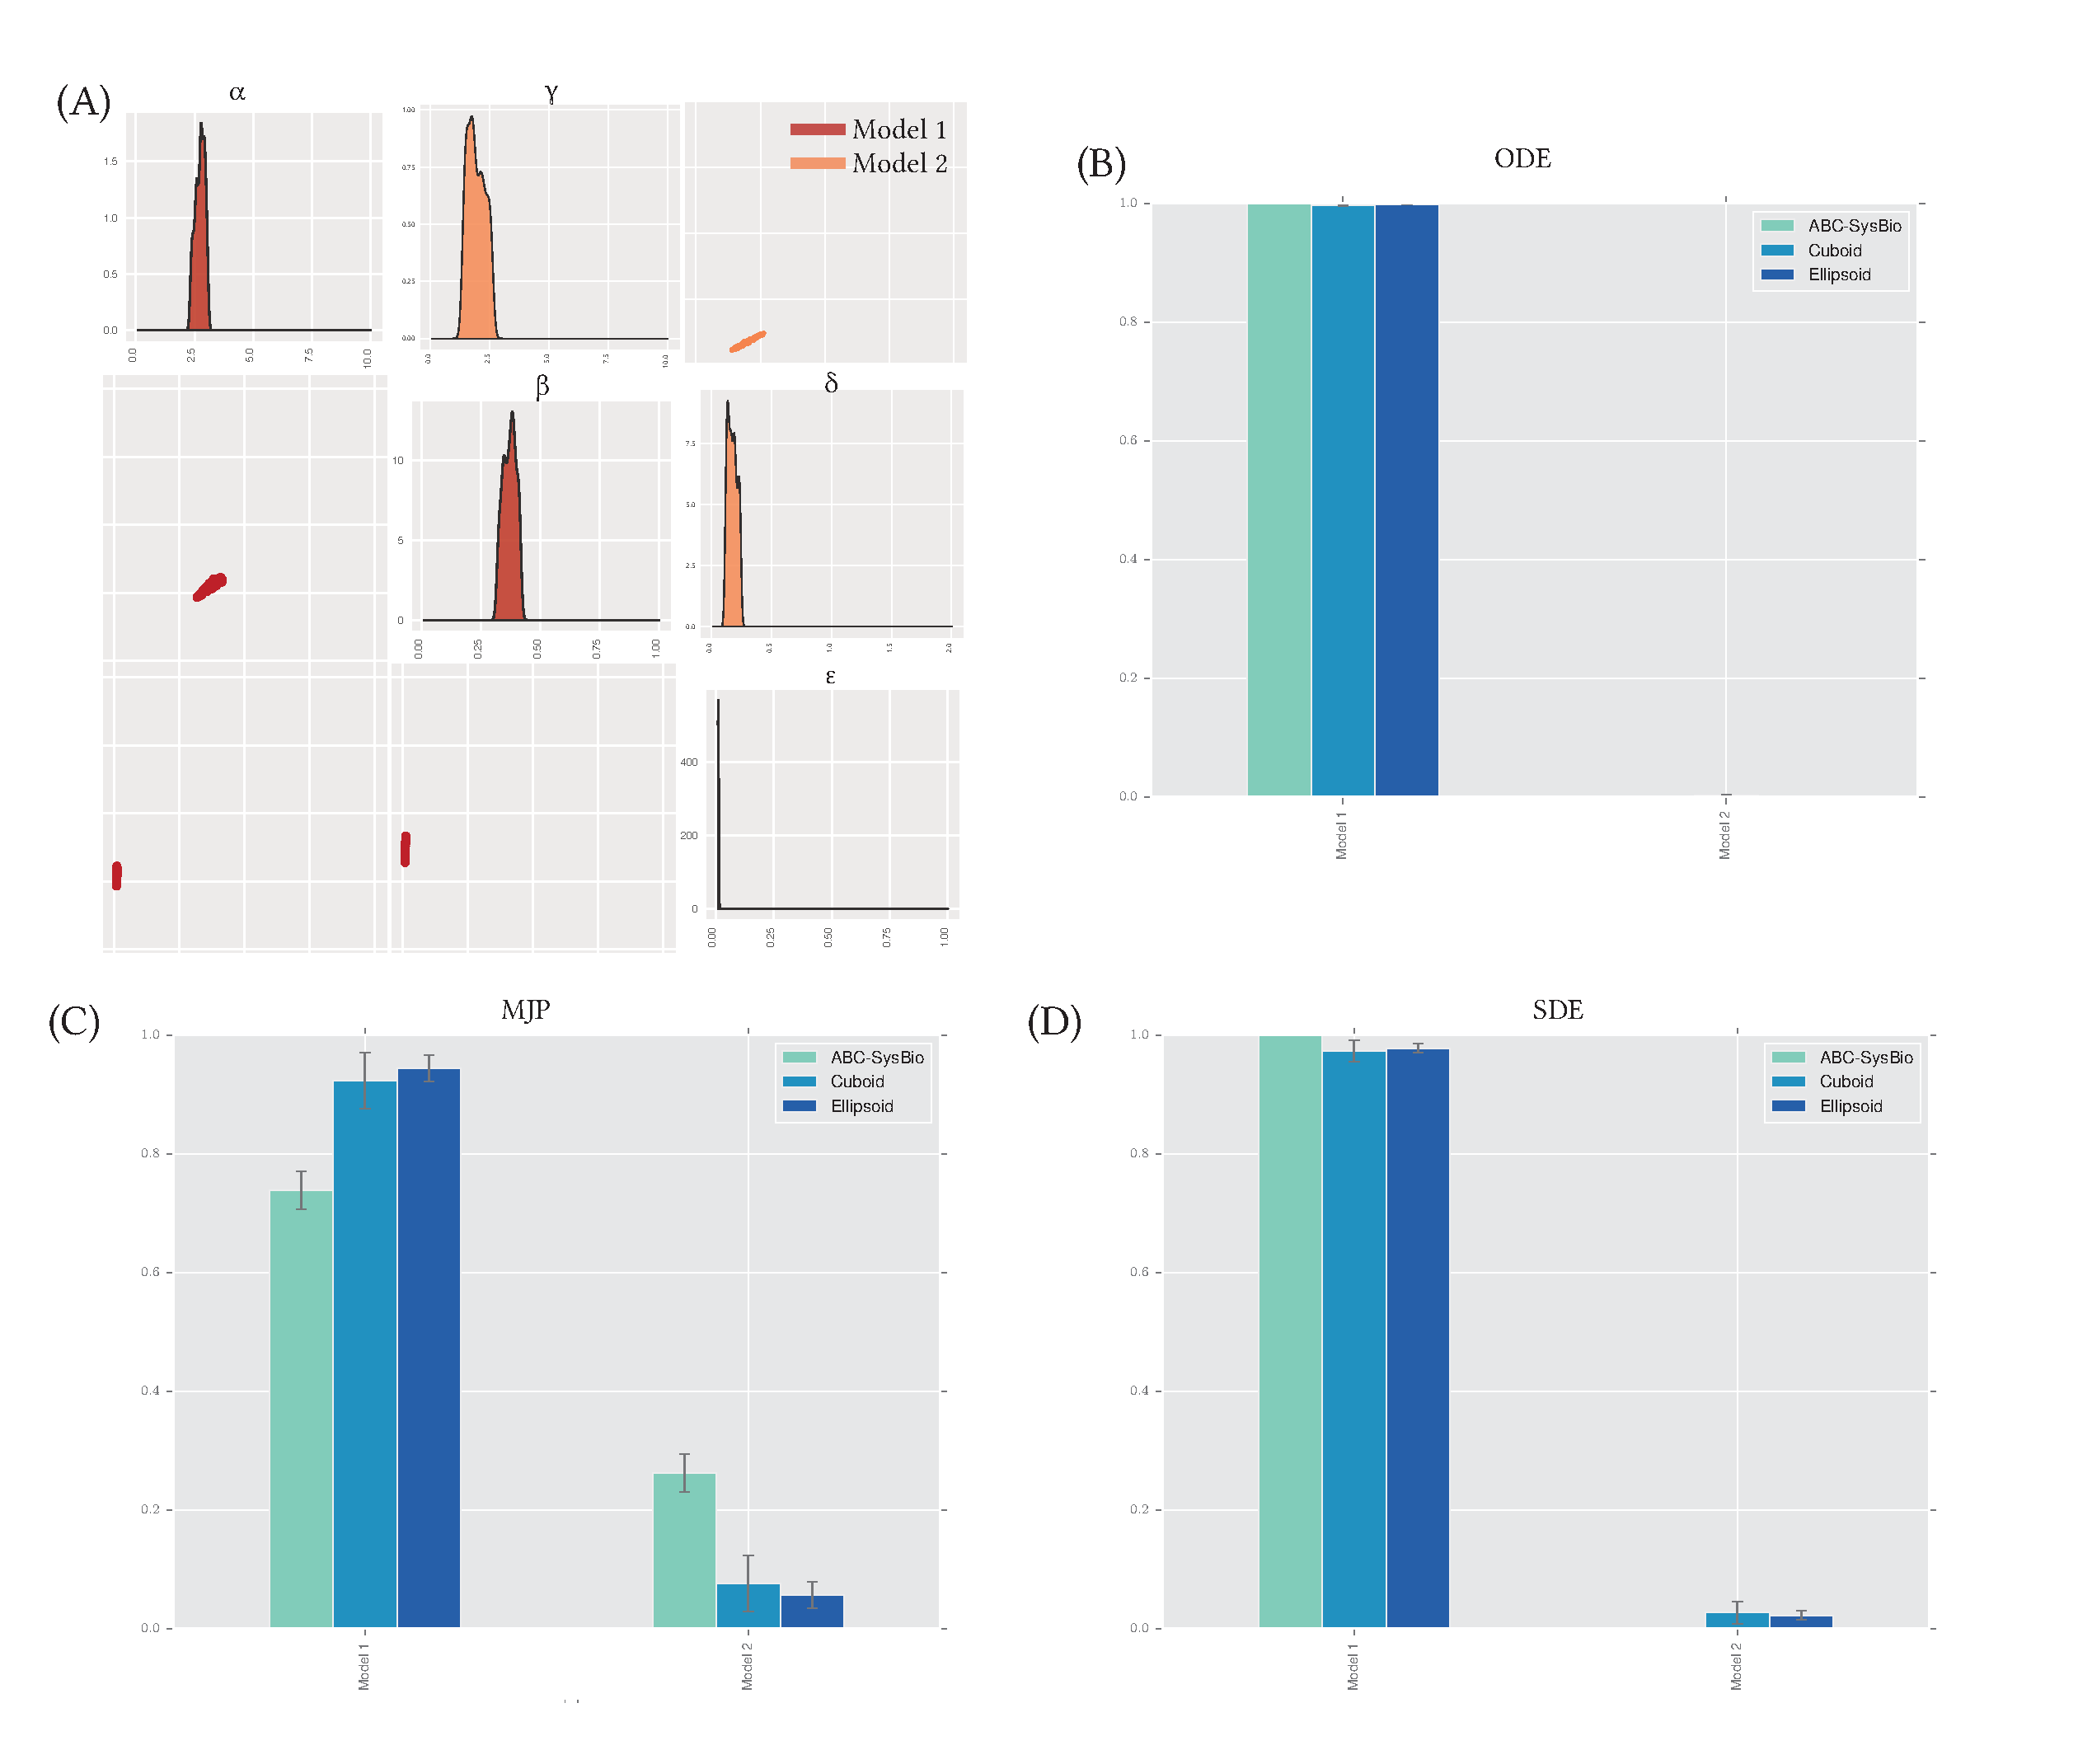
\includegraphics[width=\textwidth]{../../chapters/chapterStabilityFinder/images/ex1_sum.png}
\caption[Robustness analysis of case study 1]{\label{fig:rob_sysbio1} Robustness analysis of the three models for the spread of infectious diseases. (A-C) The posterior distributions of the three models compared. (D) I use three methods to calculate robustness, ABC-SysBio model selection, the volume of the hyper-cuboid approximation of the posterior distribution and the volume of the hyper-ellipsoid approximation of the posterior distribution. Each analysis was repeated three times. The height of the bars indicate the mean robustness from the three repeats and the error bars represent the standard deviation. There is good agreement between all three methods. All three methods show that Model 1, the simplest model, is the most robust model. }

\end{center}
\end{figure*}

\begin{figure*}[p]
\begin{center}
\includegraphics[width=\textwidth]{../../chapters/chapterStabilityFinder/images/Example4_summ.png}
\caption[Robustness analysis of case study 2]{\label{fig:rob_sysbio4} Robustness comparison of two population growth models. (A) The posterior distributions of the two models. (B-D) The models were simulated using \acrshort{ode},~\acrshort{mjp} and~\acrshort{sde}. Both the cuboid and the ellipsoid approximations agree with ABC-SysBio model selection results. Each analysis was repeated three times. The height of the bars indicate the mean robustness from the three repeats and the error bars represent the standard deviation. }
\end{center}
\end{figure*}

\clearpage


The two case studies used above show that the cuboid and the ellipsoid approximation of model robustness agree with the results obtained from ABC-SysBio model selection. A point I must draw attention to is that for ABC-SysBio model selection where model selection is incorporated in the process, each model is also considered a particle with an associated weight~\autocite{Toni:2009tr}. If a model is performing poorly it does not proceed in the algorithm and is dropped when the weight falls low enough so that the model is not sampled~\autocite{Toni:2009tr}. This can save time in the analysis as computational resources are not wasted on 'dead' models, models that perform the required behaviour poorly. Using StabilityFinder for model selection, each model must reach the given final \textepsilon{} in order for the cuboid and ellipsoid methods to be valid. This means that time and computational power will be spent on models that are potentially a bad fit, or that have posterior distributions so small compared to the prior that it will take a long time for StabilityFinder to find it. Despite this, the results agree between the all three methods of model selection. This shows that the requirement for all models to reach the final \textepsilon{} does not affect the results for the models used in the above case studies. The potentially wasted computational resources on 'dead' models is a compromise made in order to be able to run the models separately, as model selection is not the primary purpose of StabilityFinder. 

\section{Applications of StabilityFinder}

In this section I apply StabilityFinder to toggle switch models in order to find the design principles underlying their stabilities. First I apply it to a simple model with known results, the~\textcite{Gardner:2000vha} toggle switch. This model can serve as a test for StabilityFinder, as the conditions for bistability are derived in~\textcite{Gardner:2000vha}.


\subsection{StabilityFinder used on the Gardner toggle switch}
\label{sec:gard}
\textcite{Gardner:2000vha} constructed the first synthetic genetic toggle switch~\autocite{Gardner:2000vha}. Their model consisted of two mutually repressing transcription factors, as shown in Figure~\ref{fig:gard_mod}A, and in the deterministic case is defined by the following \acrshort{ode}s:

\begin{align}
\frac{du}{dt} &= \frac{a_1}{1+v^{\beta}} - u\\
\frac{dv}{dt} &= \frac{a_2}{1+u^{\gamma }} - v,
\end{align}
\noindent where \textit{u} is the concentration of repressor 1, \textit{v} the concentration of repressor 2, $a_1$ and $a_2$ denote the effective rates of synthesis of repressors 1 and 2 respectively, β is the cooperativity of repression of promoter 1 and γ of repressor 2. \textcite{Gardner:2000vha} studied the deterministic case and concluded that there are two conditions for bistability for this model; that $a_1$ and $a_2$ are balanced and that β, γ \textgreater 1 \autocite{Gardner:2000vha}. I test StabilityFinder by using it to find the posterior distribution for which this model exhibits bistable behaviour. Therefore, the desired behaviour is set to two steady states, and using a wide range of values as priors as shown in Table~\ref{tab:gard_det_stoch}, I used StabilityFinder to find the parameter values necessary for bistability to occur. The posterior distribution calculated by StabilityFinder for the Gardner deterministic case is shown in Figure~\ref{fig:gard_post}A.

\begin{table}[htbp]
\centering
\caption{Gardner switch priors in the deterministic and stochastic cases}
\label{tab:gard_det_stoch}
\begin{tabular}{@{}cccccc@{}}
\toprule
\multicolumn{4}{c}{Parameters (time\textsuperscript{-1})}                          & \multicolumn{2}{c}{Species (μM)} \\ \cmidrule(lr){1-4}
\cmidrule(lr){5-6}
$a_1$ & $\beta$ & $a_2$ & \multicolumn{1}{c}{$\gamma$} & $s_1$        & $s_2$        \\
0-60  & 0-5     & 0-60  & 0-5                           & 0-100        & 0-100        \\ \bottomrule
\end{tabular}
\end{table}

These results agree with the results reported by~\textcite{Gardner:2000vha}. For this switch to be bistable $a_1$ and $a_2$ must be balanced while β and γ must both be \textgreater 1, as can be seen in the marginal distributions of β and γ in Figure~\ref{fig:gard_post}A.

I next applied StabilityFinder to the case of the Gardner switch under stochastic dynamics using the same priors as the deterministic case, and again searched the parameter space for bistable behaviour. The posterior distribution is shown in Figure~\ref{fig:gard_post}B. We can see that the conditions on the parameters required for bistability in the deterministic case generally still stand in the stochastic case. There appears to be slightly looser requirements on the parameters of the stochastic model (wider marginal distributions). Some difference between the deterministic and stochastic posteriors is expected as different clustering algorithms are used for the stochastic and the deterministic cases. The Gap statistic is used in the case of the stochastic case, as it is capable of dealing with noisier data whereas a simpler and faster algorithm is used for clustering the deterministic solutions. These results demonstrate that StabilityFinder can be used to find the parameter values that can produce a desired stability and can be confidently applied to more complex models.


\begin{figure*}[htbp]
\begin{center}
	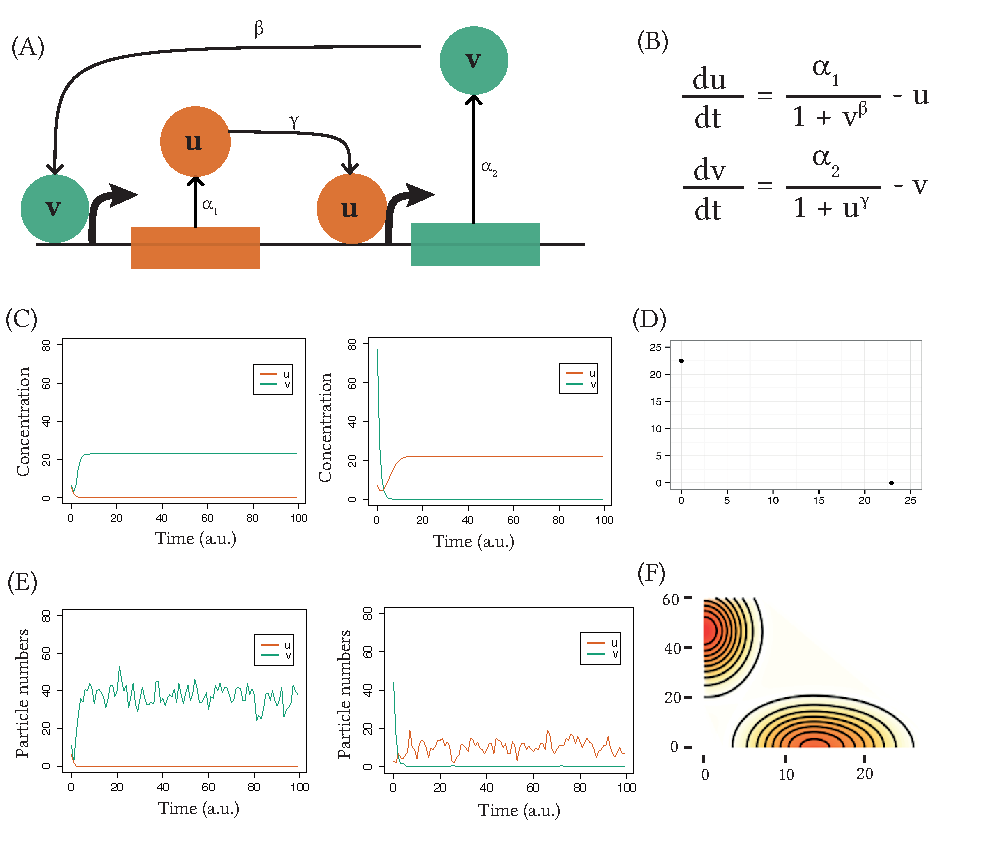
\includegraphics[scale=0.8]{../../chapters/chapterStabilityFinder/images/gardner_poste.pdf}
	\caption[StabilityFinder used on the Gardner toggle switch]{\label{fig:gard_mod} The Gardner switch model used to test StabilityFinder. The Gardner model (A) consists of two mutually repressing transcription factors. (B) It can be reduced to a two-equation system, where $u$ and $v$ are the two transcription factors, $a_1$,$a_2$ are their effective rates of synthesis, $u$, $v$ are their concentrations and $\beta$, $\gamma$ represent the cooperativity of each promoter. (C) Two samples of deterministic simulated time courses of the Gardner switch and (D) The resulting phase plot. (E) Two samples of time courses of the stochastic simulations and (F) the resulting stationary distributions.}
\end{center}
\end{figure*}

\begin{figure*}[htbp]
\centerfloat
	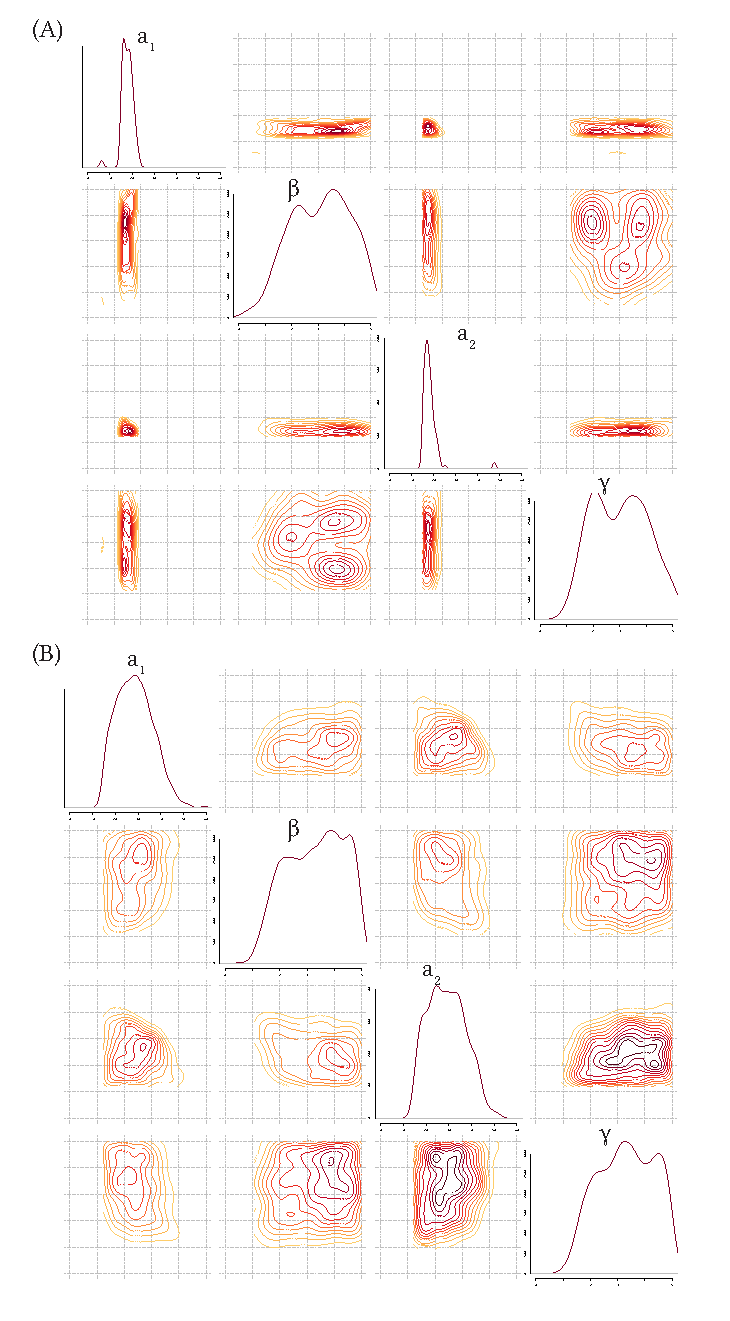
\includegraphics[width=0.8\textwidth]{../../chapters/chapterStabilityFinder/images/gardner_posterior_w.pdf}
	\caption[The posterior distributions of the bistable Gardner toggle switch]{\label{fig:gard_post} Elucidating the stability of the Gardner switch. The Gardner model has four parameters, for which I want to find the values for which this system is bistable. I use StabilityFinder to find the posterior distribution of the bistable Gardner switch, deterministically (A) and stochastically (B). The posterior distributions are shown as the density plots of each parameter as well as each one plotted against the other.  }
\end{figure*}
\clearpage
%\begin{figure*}[h]
%\begin{center}
%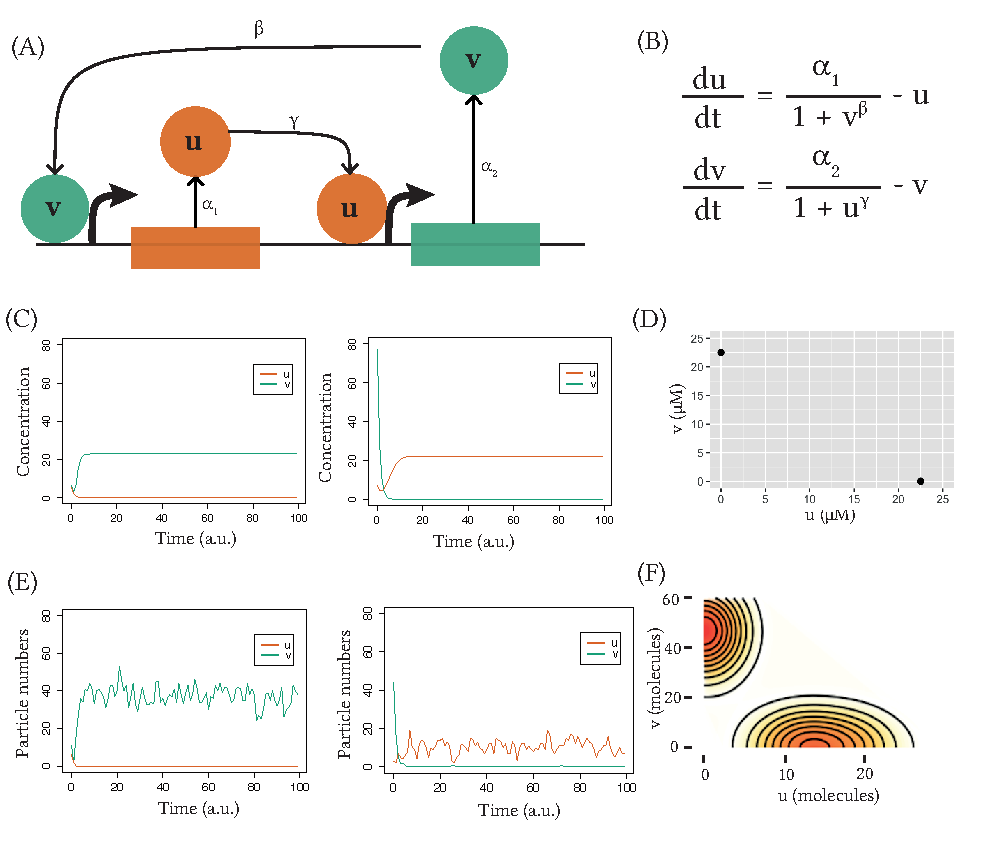
\includegraphics[width=\textwidth]{../../chapters/chapterStabilityFinder/images/gardner_poster.png}
%\caption[LoF caption]{ \label{fig:fig2}: Elucidating the stability of the Gardner switch. The Gardner model (A) consists of two mutually repressing transcription factors. It can be reduced to a two-equation system, where $u$ and $v$ are the two transcription factors, $a_1$,$a_2$ are their effective rates of synthesis, $u$,$v$ are their concentrations and $\beta$, $\gamma$ represent the cooperativity of each promoter. There are four parameters in the model, for which we want to find the values for which this system is bistable. We use StabilityFinder to find the posterior distribution of the bistable Gardner switch, deterministically (B) and stochastically (C). The posterior distributions are shown as the density plots of each parameter as well as each one plotted against the other. }
%\end{center}
%\end{figure*}
%\clearpage


\subsection{Lu toggle switch models}
\label{sec:lu}
Next I analyzed an extension of the Gardner switch model developed by~\textcite{Lu:2014kc}. I use these models as they are of increased complexity from the Gardner model. \textcite{Lu:2014kc} considered two types of switches, the classic switch consisting of two mutually repressing transcription factors (model \acrshort{cs-lu}), as well as a double positive switch \acrshort{dp-lu}.  The \acrshort{cs-lu} switch was found to be bistable given the set of parameters used, while the \acrshort{dp-lu} switch was found to be tristable~\autocite{Lu:2014kc}. The \acrshort{cs-lu} model used in their study is given by the following system of \acrshort{ode}s, as given in~\textcite{Lu:2014kc}.

\begin{align}
\dot{x} & = g_{x}\, H^{S}_{xy}(y) -k_{x}x \\
\dot{y} & = g_{y}\,H^{S}_{yx}(x) -k_{y}y,
\end{align}

\noindent where:

\begin{align}
H^{S}_{I}(x) &= H^{-}_{I}(x)+\lambda_{I}H^{+}_{I}(x) \\
H^{-}_{I}(x) &= 1 \big/\left[1+(x/x_{I})^{n_{I}}\right] \\
H^{+}_{I}(x) &= 1-H^{-}_{I}(x),
\end{align}

\noindent and the \acrshort{dp-lu} model is given by
\begin{align}
\dot{x} = f_{x}(x,y) &= g_{x}\, H^{S}_{xy}(y)\, H^{S}_{xx}\,(x)-k_{x}x \\
\dot{y} = f_{y}(x,y) &= g_{y}\,H^{S}_{yx}(x)\,H^{S}_{yy}\,(y)-k_{y}y,
\end{align}

\noindent $g_I$ represents the production rate, $k_I$ the degradation rate, $n_I$ the Hill coefficient, $x_I$ the Hill threshold concentration and $\lambda_I$ the fold change of the transcription rates, and $I\in\{xy, yx, xx, yy\}$.

For the parameter values used in the Lu study, the \acrshort{cs-lu} switch exhibits three steady states, two of which are stable and one is unstable. The \acrshort{cs-lu} switch exhibits five steady states, of which three are stable and two are unstable. Bifurcation diagrams of the two Lu models are shown in Figure~\ref{fig:lu_bifurc}. 


\begin{figure*}[htbp]
\begin{center}
	\includegraphics[scale=0.5]{../../chapters/chapterStabilityFinder/images/lu_bifurc.png}
	\caption[Phase plane analysis of the Lu toggle switch models]{\label{fig:lu_bifurc}  Stream plot of the vector plot of the (A) \acrshort{cs-lu} and (B) \acrshort{dp-lu} switches. The colours indicate the magnitude of the vectors, with yellow indicating high and red low values. The blue points represent stable steady states and the grey points represent unstable steady states.  }
\end{center}
\end{figure*}
\clearpage
 
\subsubsection{Extending the Lu models}

I start the analysis of the Lu models by extending their analytical approach to solving the system. I use StabilityFinder to explore a larger parameter space which allows us to distinguish between rare events and robust behaviours. The advantage of using StabilityFinder over solving the system analytically is that the full parameter space is explored rather than solving the system for a single set of parameters. This allows us to deduce model properties that could not otherwise be identified. Robustness to parameter fluctuations can be explored, as well as parameter correlations and restrictions on the values they can take while still producing the desired behaviour. 

It is known that that the addition of positive autoregulation to the classical toggle switch can induce tristability~\autocite{Lu:2014kc}. Here I investigate the interplay of positive autoregulation on the values of the other parameters in the model. I extended the analysis presented in~\textcite{Lu:2014kc} by including the switch with single positive autoregulation (model \acrshort{sp-lu}), where an asymmetry of positive feedbacks is present between the two genes. The three switches considered in this analysis are shown in Figure~\ref{fig:lu_mods}. The \acrshort{sp-lu} switch is modelled using the following \acrshort{ode} system


\begin{figure*}[tb]
\begin{center}
	\includegraphics[width=\textwidth]{../../chapters/chapterStabilityFinder/images/LU_diagrams.png}
	\caption[The three Lu toggle switch models.]{\label{fig:lu_mods} The three LU toggle switch models. (A) \acrshort{cs-lu}, (B) \acrshort{sp-lu} and (C) \acrshort{dp-lu}.   }
\end{center}
\end{figure*}



\begin{align}
\dot{x} & = g_{x}\, H^{S}_{xy}(y)\, H^{S}_{xx}\,(x)-k_{x}x \\
\dot{y} & = g_{y}\,H^{S}_{yx}(x) - k_{y}y.
\end{align}


Using StabilityFinder with priors centred around the parameter values used in the original paper (see Table~\ref{tab:lu_all}), we can identify the most important parameters for achieving the models' stability. The phase plots of the final populations of the models are shown in Figure~\ref{fig:lu_paper_phase} and the posterior distribution of these models are shown in Figure~\ref{fig:fig3}A. We find that the parameters representing the rates of degradation of the transcription factors in the system ($k_x$, $k_y$) must both be large in relation to the prior ranges for bistability to occur. Protein degradation rates have been shown to be important for many system behaviours including oscillations \autocite{Woods:2016eh}.

\begin{table}[htpb]
\centering
\caption{Priors of the classical (\acrshort{cs-lu}), single positive (\acrshort{sp-lu}) and double positive (\acrshort{dp-lu}) models.}
\label{tab:lu_all}
\begin{tabular}{@{}ccccc@{}}
\toprule
Parameter                                            & Symbol & \acrshort{cs-lu}        & \acrshort{sp-lu}         & \acrshort{dp-lu}       \\ \midrule
\multirow{2}{4cm}{Production rate (Proteins/Minute)}                & gx        & 30-50   & 1-2       & 1-100    \\
                                                & gy        & 30-50   & 20-25     & 1-100    \\[4pt]
\multirow{2}{4cm}{Degradation rate (Minute-1)}               & kx        & 0-0.5   & 50-55     & 0-1      \\
                                                & ky        & 0-0.5   & 48-52     & 0-1      \\[4pt]
\multirow{2}{4cm}{Hill coefficient}               & nxy       & 1-5     & 30-35     & 0-10     \\
                                                & nyx       & 1-5     & 0.1-0.2   & 0-10     \\[4pt]
\multirow{2}{4cm}{Hill thresholds concentration (Proteins)}  & xxy       & 100-300 & 2-3       & 100-1000 \\
                                                & xyx       & 100-300 & 0.4-0.6   & 100-1000 \\[4pt]
\multirow{2}{4cm}{Transcription rate fold change} & lxy       & 0-0.5   & 0.02-0.04 & 0-1      \\
                                                & lyx       & 0-0.5   & 0.02-0.04 & 0-0.2    \\[4pt]
\multirow{2}{4cm}{Hill coefficient}               & nXX       & -       & 25-30     & 0-10     \\
                                                & nYY       & -       & 0.01-0.02 & 0-10     \\[4pt]
\multirow{2}{4cm}{Hill thresholds concentration (Proteins)}  & xXX       & -       & 0.4-0.5   & 50-500   \\
                                                & xYY       & -       & 1-3       & 50-500   \\[4pt]
\multirow{2}{4cm}{Transcription rate fold change} & lXX       & -       & 65-72     & 1-20     \\
                                                & lYY       & -       & 0.02-0.04 & 1-20     \\ \hline
\end{tabular}
\end{table}



\begin{figure*}[p]
\begin{center}
\includegraphics[width=\textwidth]{../../chapters/chapterStabilityFinder/images/lu_paper_phase.png}
\caption[Resulting phase plots from StabilityFinder used on the Lu switches ]{ \label{fig:lu_paper_phase}The phase plots of 100 particles from the last population of the three Lu switches. (A) The bistable \acrshort{cs-lu} (B) The bistable \acrshort{sp-lu} and (C) The tristable \acrshort{dp-lu}. There are two types of tristable behaviour, one where the third steady state is zero-zero and one where the third state is high (non-dead). }
\end{center}
\end{figure*}
\clearpage

\begin{figure*}[p]
\centerfloat
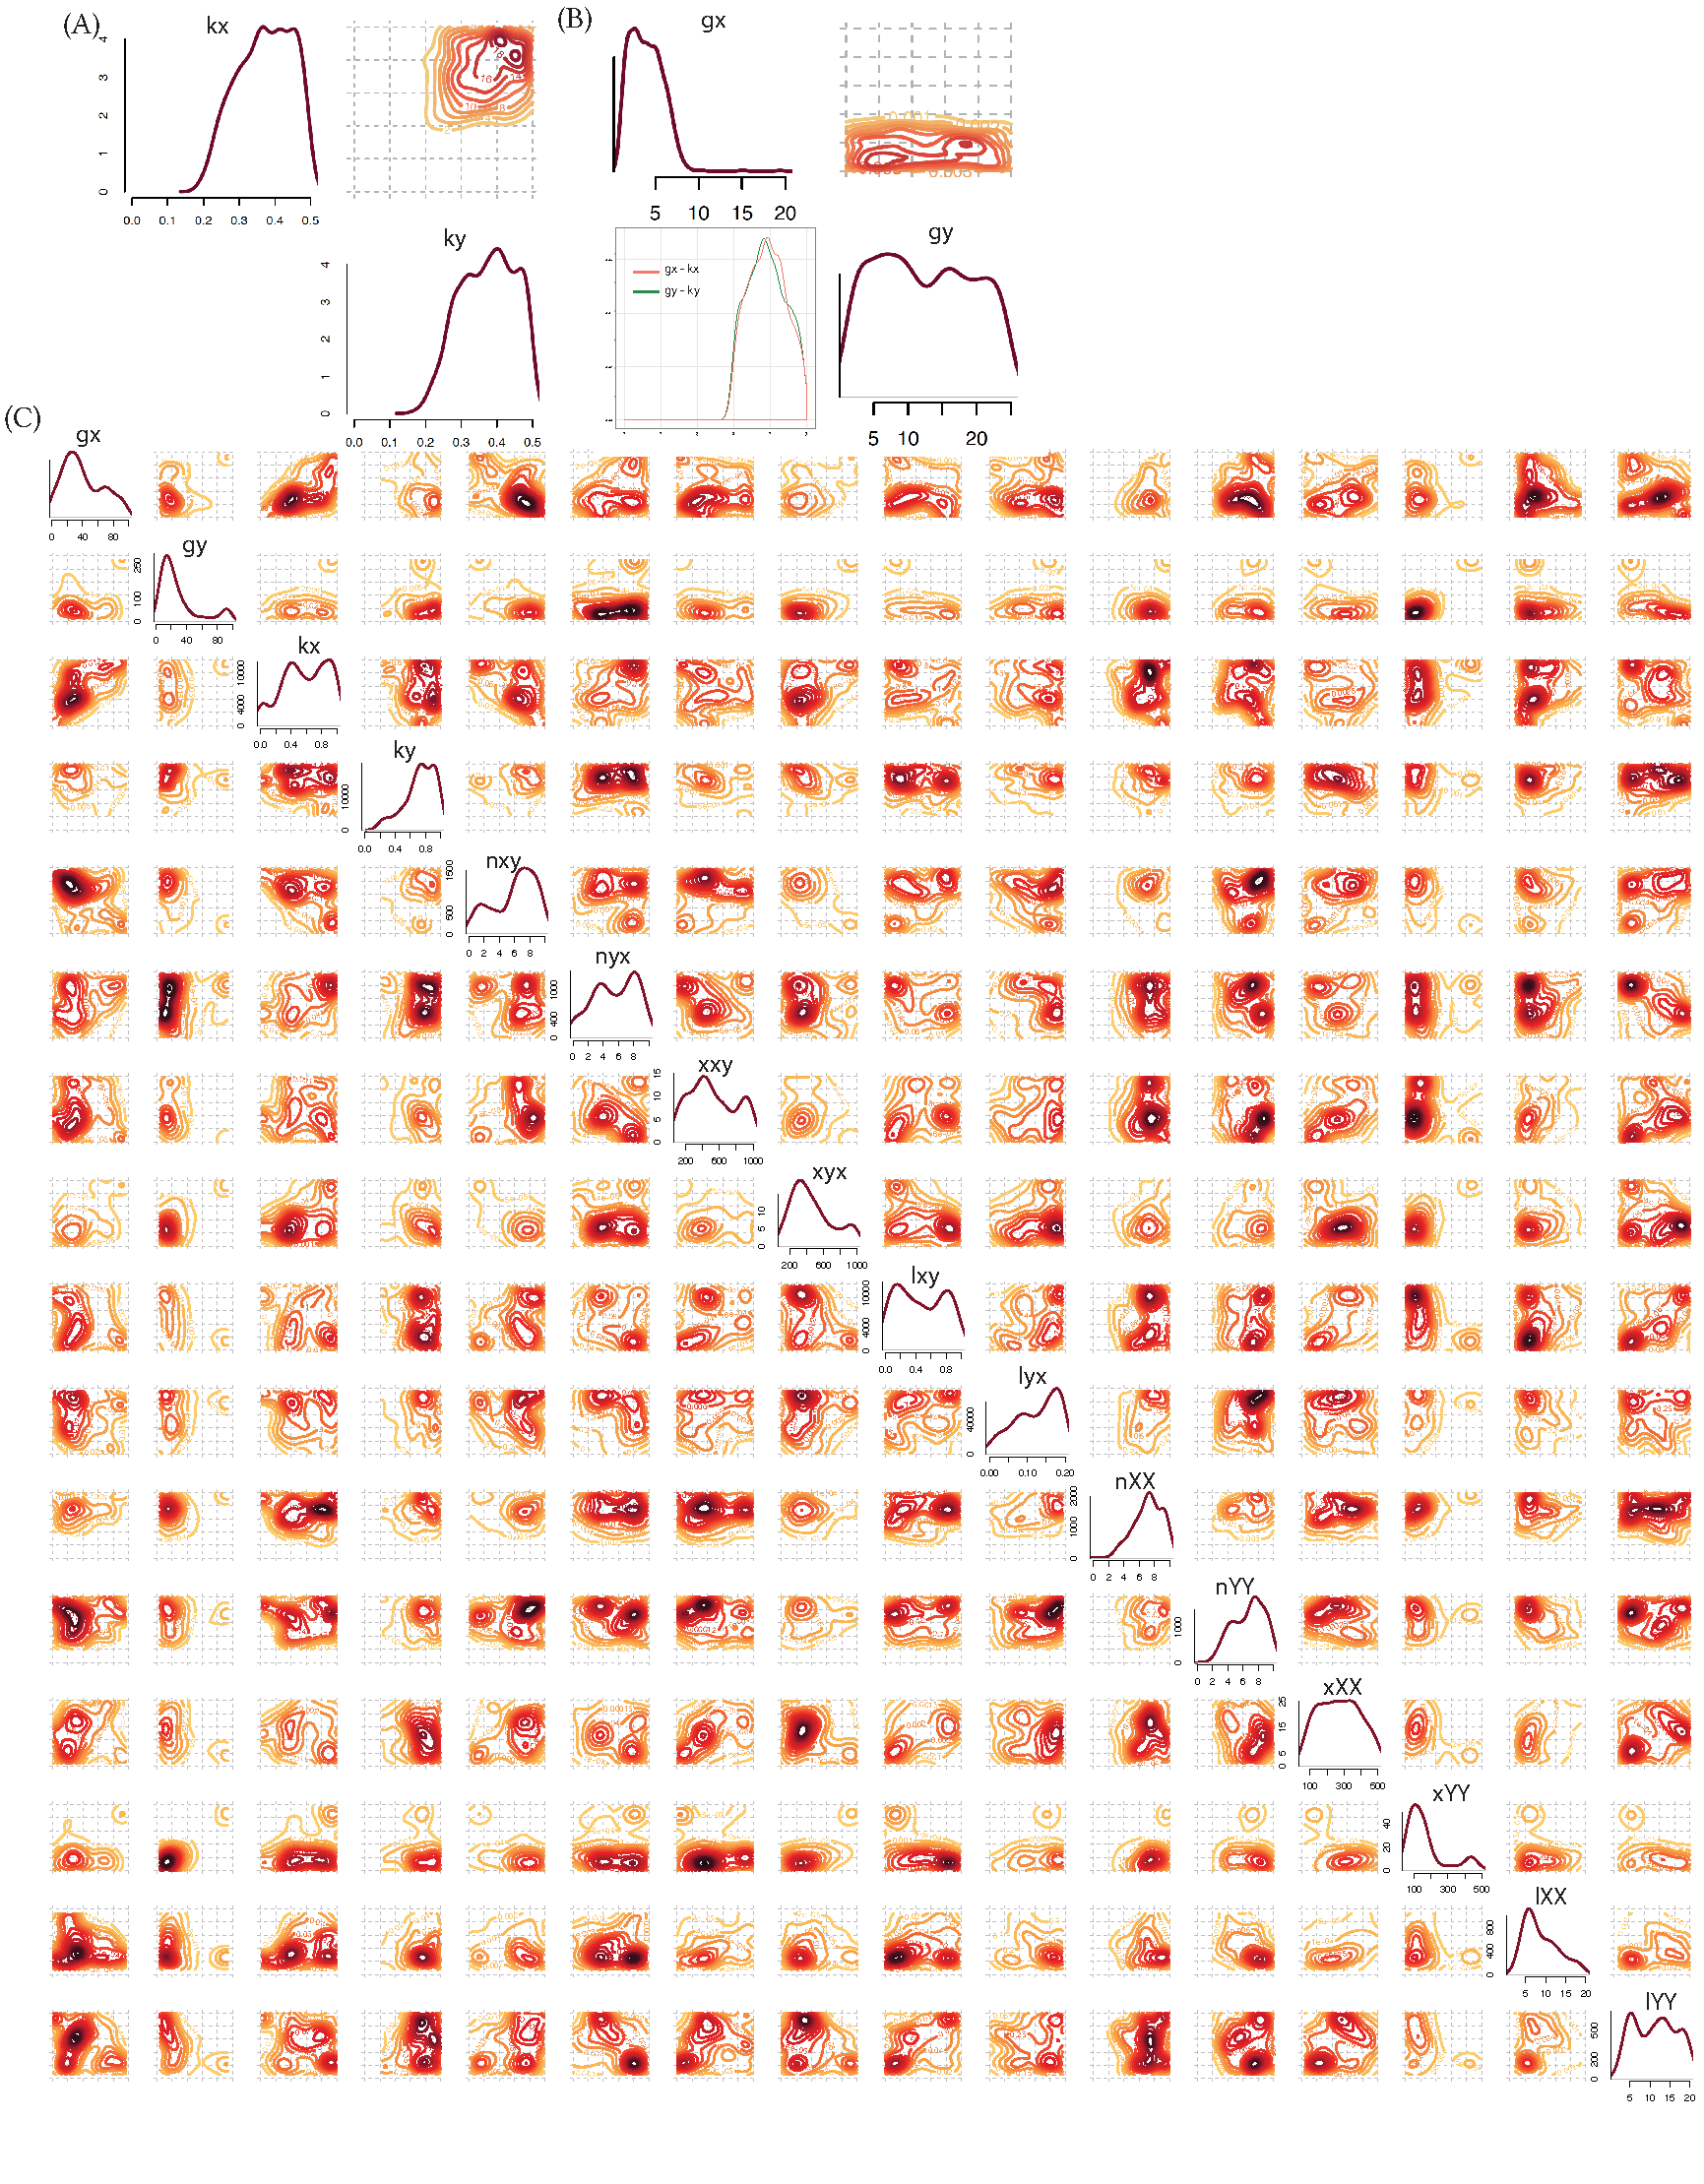
\includegraphics[width=1.3\textwidth]{../../chapters/chapterStabilityFinder/images/lu_paper_post_w.pdf}
\caption[Posterior distributions of the Lu switches]{ \label{fig:fig3}The three variants of the Lu models. (A) The \acrshort{cs-lu} switch is bistable. The most restricted parameters for this behaviour are $kx$ and $ky$ which both have to be high relative to the prior. (B) The extended Lu model with a single positive autoregulation on $X$. This model is bistable when $gx$ is small, but the net production of protein is equal for the two nodes. (C) The Lu model with double positive autoregulaiton is tristable, and its posterior distribution shown here. }

\end{figure*}
\clearpage

We find that the switch with single positive autoregulation is capable of bistable behaviour as seen in Figure~\ref{fig:fig3}B, but this is only possible when the strength of the promoter under positive autoregulation, $gx$, is small (Figure \ref{fig:fig3}). There appear to be no such constraints on the strength of the original, unmodified, promoter, $gy$.  

Upon examination of the \acrshort{dp-lu} model, we also find that tristability in the switch is relatively robust, as tristability is found across a large range of parameter values, with no parameters strongly constrained. Two types of tristable behaviour are identified, one where the third steady state is at (0,0) and and one where the third steady state has non-zero values, as seen in Figure~\ref{fig:lu_paper_phase}. This result agrees with previous work by~\textcite{Guantes:2008gs}, who found that a switch can exhibit two kinds of tristability, one in which the third steady state is high (\RNum{3}$_H$) and one in which it is low (\RNum{3}$_L$)~\autocite{Guantes:2008gs}. %The difference between the two tristable switches is explored in a later section. 

%%%OP EDO PAME GIA BI TRI &&&&
%deterministic dynamics~\autocite{Guantes:2008gs}. The classical switch is also capable of both bistable and tristable behaviour when stochastic dynamics capture small number effects~\autocite{Ma:2012dt}. It is therefore of great interest to understand the conditions under which these two behaviours occur in both stochastic and deterministic scenarios. 
\subsubsection{Multistability in the Lu models}
\label{sec:lu_234}
The DP switch is capable of both bistable and tristable behaviour as well as 4 coexisting states under deterministic dynamics (quadristability)~\autocite{Guantes:2008gs}. It is of great interest to understand the conditions under which these three behaviours occur. A bifurcation analysis of the DP switch was carried out using the PyDSTool~\autocite{Clewley:2012kj} in order to get an indication of the stabilities this model is capable of, and at which parameter ranges these are found.

Since the Lu models can be solved analytically, the bifurcation diagram of the \acrshort{dp-lu} can be obtained by keeping all parameters constant apart from gene expression ($gx$). The result shown in Figure~\ref{fig:lu_234}B, the system can exhibit 2, 3 or 4 steady states depending on the value of the gene expression rate. We observe that if $100 \leq gx\leq 120$ the system exhibits four steady states, if $9 \leq gx\leq 10$ the system is tristable and if $10 \leq gx\leq 100$ the system is bistable. I use the whole range tested above ($0 \leq gx\leq 140$) as prior distributions in StabilityFinder and searched parameter space for 2, 3 and 4 steady states.

Using StabilityFinder a more complex picture of the parameter space that can produce each behaviour can be obtained. This is because, unlike the bifurcation analysis, StabilityFinder does not require any of parameters to be fixed. Since there are no such restraints on the value each parameter can take we obtain a bigger range of parameters that can produce each behaviour than the ranges found during the bifurcation analysis. The priors used for each analysis are identical and include the whole range of values found in the bifurcation diagram, varying only the required number of steady states. In addition, unlike the bifurcation analysis the values for $gx$ and $gy$ are not forced to be equal in the analysis done on StabilityFinder.

%In order to do this using StabilityFinder, we first obtained posterior distributions for bistable and tristable behaviours in the deterministic case (\acrshort{dp-lu} model) and then compared the individual parameter distributions (Figure~\ref{fig:fig6} and Supplementary Information). From analysis of the one dimensional marginal distributions it appears that there is no difference in the parameter values that allow a switch to be bistable versus tristable (Figure~\ref{fig:fig6}B). However, upon examination of the two dimensional marginal distributions we find that the correlation structure of a small subset of the posterior parameter values is in fact different under the two behaviours (Figure~\ref{fig:fig6}C). Most notably, we find differences in the bivariate distribution of the two parameters for gene expression, $gx$ and $gy$, as highlighted in Figure~\ref{fig:fig6}C, box 1. In the tristable case the distribution is more constrained than in the bistable case, as both parameters must be small for tristability to arise. 



\begin{figure*}[htbp]
	\centerfloat
		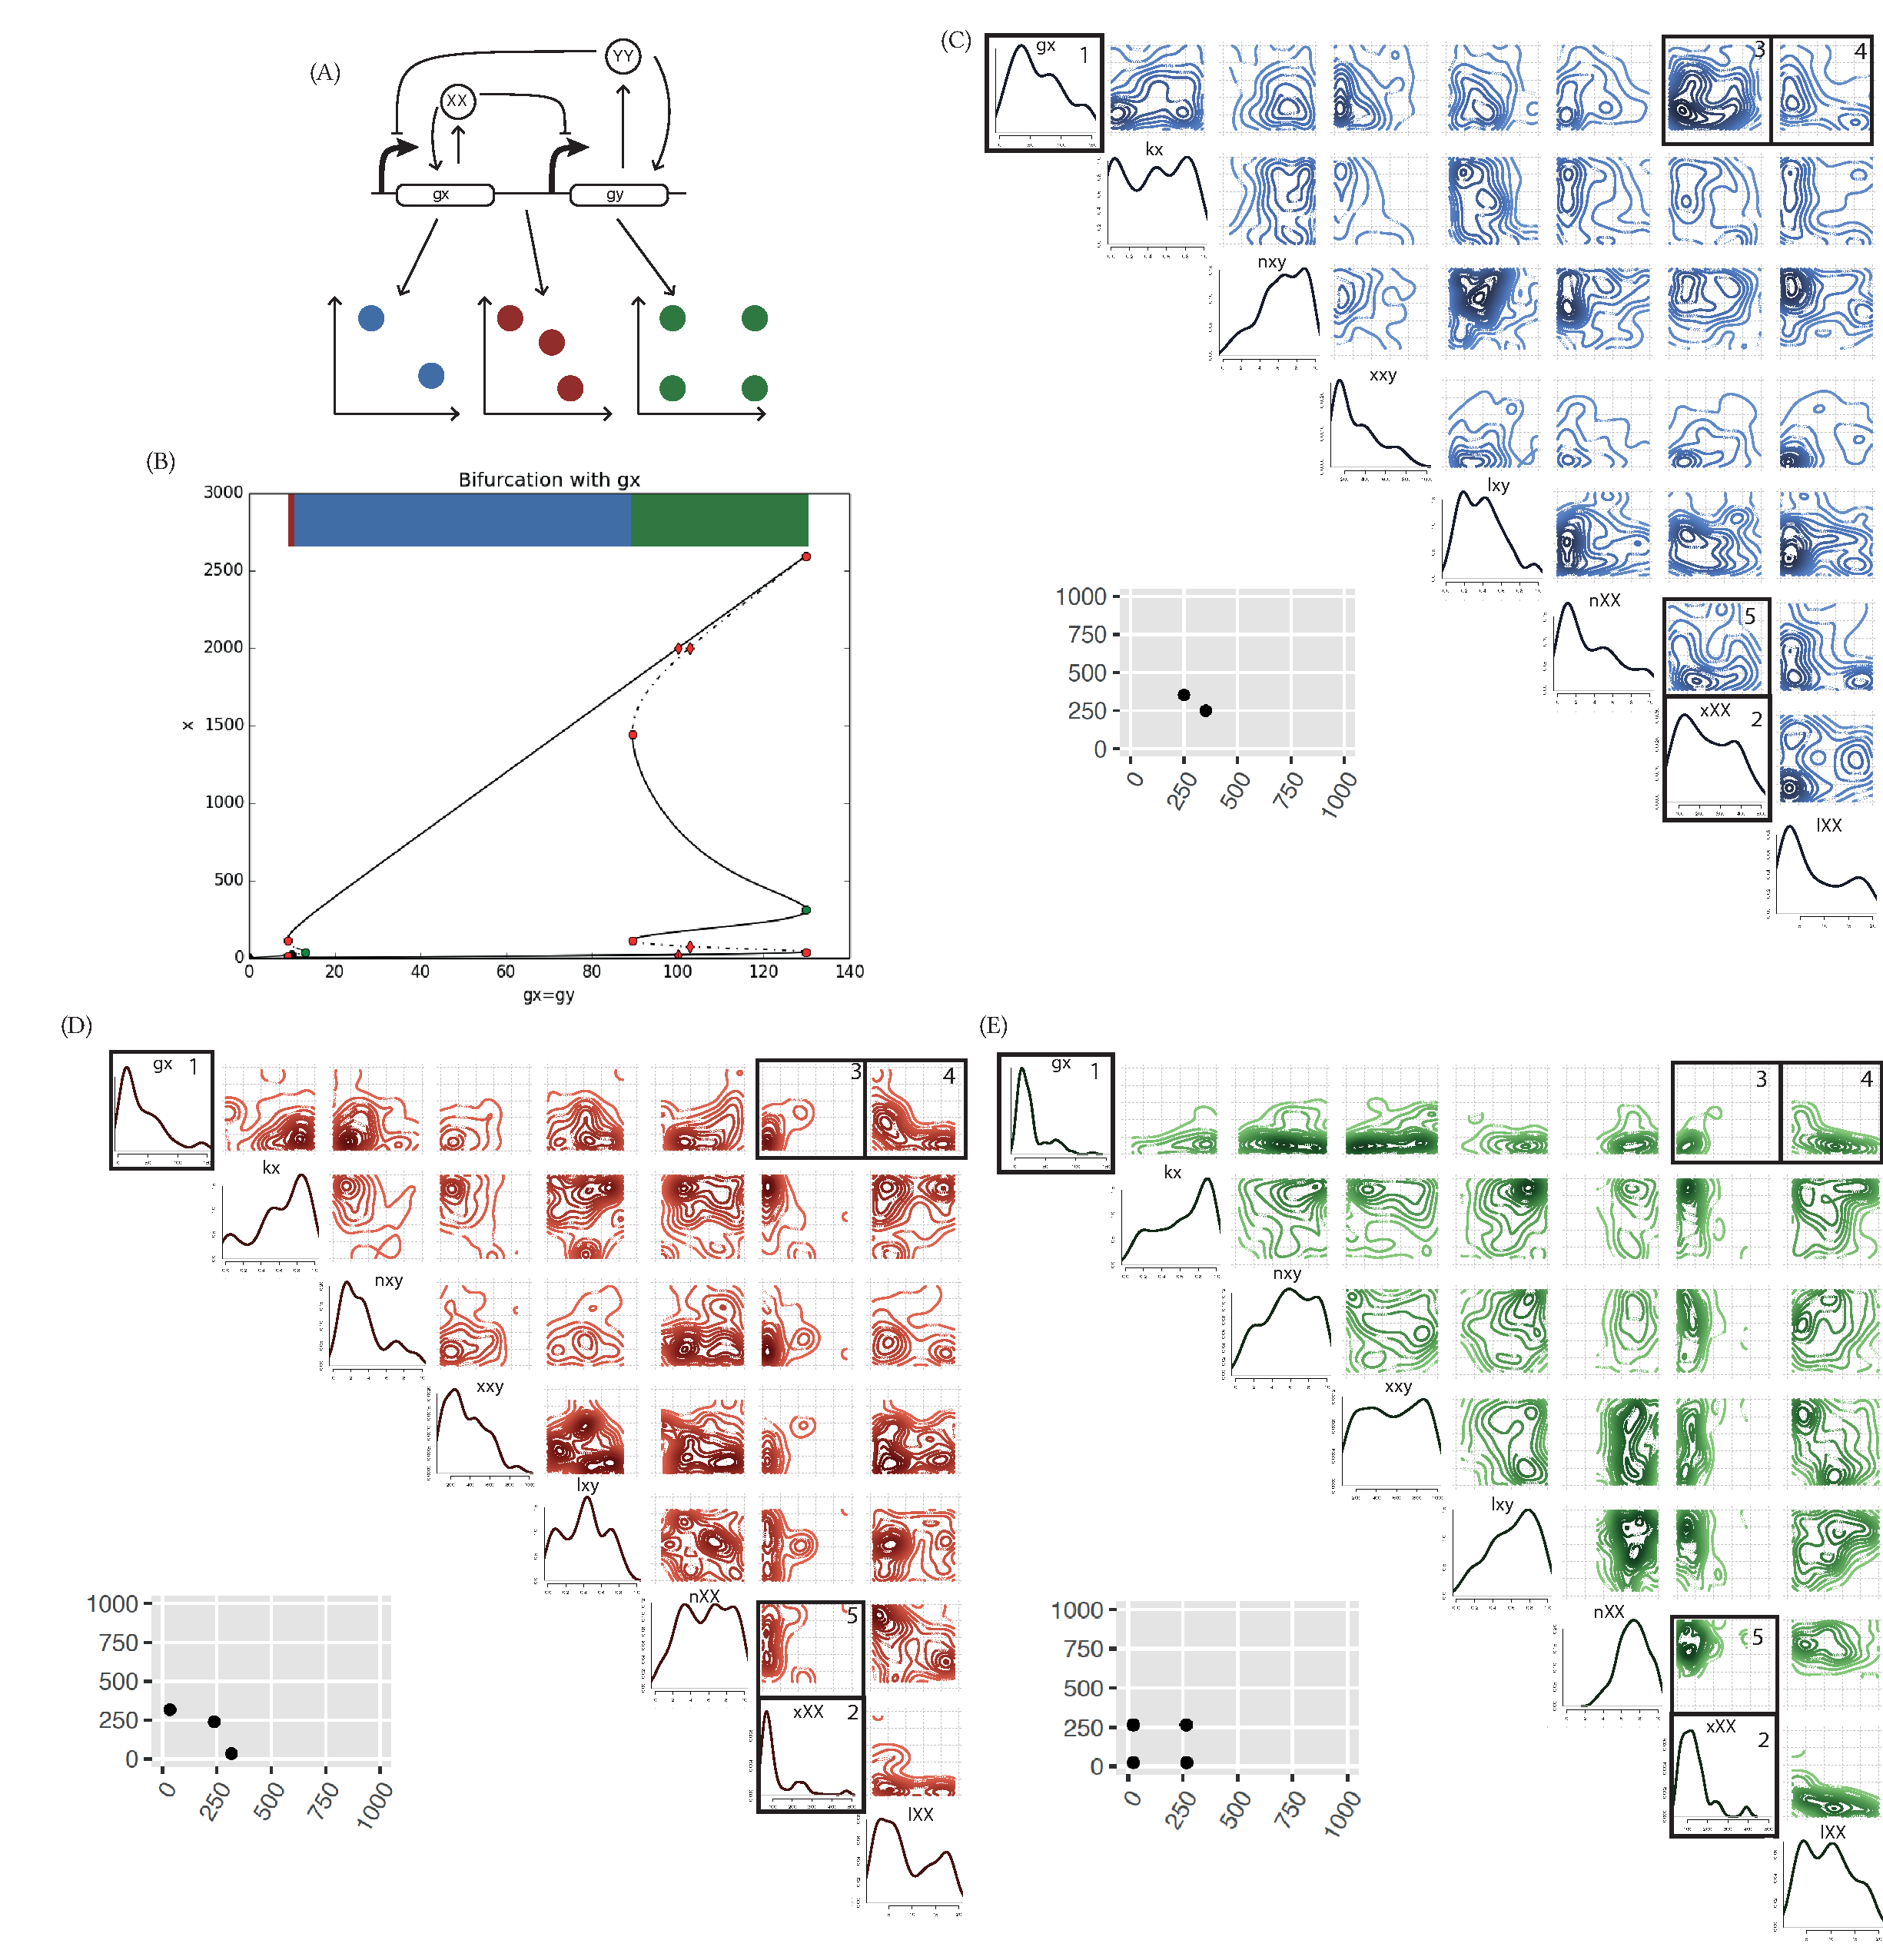
\includegraphics[width=1.2\textwidth]{../../chapters/chapterStabilityFinder/images/Lu_234_w.pdf}
		\caption[ Design principles of multistable switches]{ \label{fig:lu_234}Design principles of multistable switches. (A) Using the Lu model with added positive autoregulation we uncover the design principles dictating if a switch will be bistable, tristable, or will have 4 steady states. (B-D) By considering the bivariate distributions of the parameters we can uncover the differences in the parameters of a bistable switch compared to a tristable switch, compared to a quadristable switch . The posterior distribution of the bistable switch is shown in purple, of the tristable switch in red and of a quadristable in green. The bivariate distributions for which a difference is observed between the stabilities are in black boxes. An example of a phase plot from each behaviour is shown next to the corresponding posterior distribution.}
\end{figure*}

    

 Using StabilityFinder, the posterior distributions for bistable, tristable and quadristable behaviours in the \acrshort{dp-lu} model were obtained and then the posterior parameter distributions compared (Figure~\ref{fig:lu_234}). Upon examination of the posterior distributions for all three switches we observe that a subset of the posterior parameter values is different under the three behaviours. Differences are found in the univariate distribution of the parameters for gene expression, $gx$, as highlighted in Figure~\ref{fig:lu_234}, box 1. This parameter must be small for a quadristable switch to occur but there are no such restraints for a bistable or a tristable switch. Furthermore, parameter $xXX$ must be small for three and four steady states to be achieved but there are no such restraints for a bistable switch, as can be seen in Figure~\ref{fig:lu_234}, box 2. Parameter $xXX$ represents the Hill threshold concentration, and is equivalent to to the Hill constant described in Section~\ref{sec:hill}. This parameter dictates the substrate concentration at which the switch occurs. We find that the Hill constant has to be small in order to observe three or four steady states.

We also find a difference in the bivariate distributions in the posterior. Most notably, we find that parameters $xXX$ and $gX$ are tightly constrained in the tristable and the four steady state cases, where both parameters are required to be small, but less so in the bistable case (Figure~\ref{fig:lu_234}, box 3). Another notable difference is between parameters $xXX$ and $nXX$ shown in Figure~\ref{fig:lu_234}, box 5, where they are constrained in the tristable and quadristable cases but not the bistable case. There parameters represent the Hill constant and the Hill coefficient respectively. The Hill constant dictates the substrate concentration that results in half of the response, i.e. it is substrate concentration at which switching is observed. The Hill coefficient affects the steepness of the switching curve, as a higher Hill coefficient results in a steeper response, as illustrated in Figure~\ref{fig:hill_ex}.

Interestingly, we also find parameter correlations conserved between the three behaviours, as seen in Figure~\ref{fig:lu_234}, box 4, where parameters $lXX$ and $gx$, positive autoregulation and gene expression are negatively correlated in both cases.  This highlights the importance of treating unknown parameters as distributions rather than fixed values when studying the parameter values of a model, as they are capable of uncovering not only the ranges and values needed but also the correlations between parameters that would not have otherwise been detected. 






%Upon examination of the two dimensional marginal distributions we find that the correlation structure of a small subset of the posterior parameter values is in fact different under the two behaviours (Figure~\ref{fig:lu_234}). Most notably, we find differences in the bivariate distribution of the two parameters for gene expression, $gx$ and $gy$. In the tristable case the distribution is more constrained than in the bistable case, as both parameters must be small for tristability to arise. 


%Parameters $xYY$ and $gy$ are tightly constrained in the tristable case and both required to be small, but less so in the bistable case (Figure~\ref{fig:fig6}C, box 3). Another notable difference is between parameters $xXX$ and $lXX$ shown in Figure~\ref{fig:fig6}C, box 4, where they are constrained in the bistable case but not the tristable case. Interestingly, we also find parameter correlations conserved between the bistable and tristable case, as seen in Figure~\ref{fig:fig6}C, box 2, where parameters $lXX$ and $gx$, positive autoregulation and gene expression are negatively correlated in both cases.  This highlights the importance of treating unknown parameters as distributions rather than fixed values when studying the parameter values of a model, as they are capable of uncovering not only the ranges and values needed but also the correlations between parameters that would not have otherwise been detected.

I further analyse these models by studying the phase plots resulting from simulating the particles from the posterior distribution to steady state. The phase plots from 100 particles from each posterior are shown in Figure~\ref{fig:lu_234_phase}. We find that there is a strong conservation on the locations of the steady states between each particle. This indicates that the steady states in a two-node toggle switch tend to be symmetrical. This gives rise to the patterns seen in Figure~\ref{fig:lu_234_phase}. It is important to highlight that this was not set as a requirement for the behaviour of the switch in StabilityFinder, but the behaviour that these models gave rise to. There were no constraints on the level or location of the steady states. 

The symmetrical steady states are especially evident in the quadristable switch.  For every steady state at (0, 0) there is another steady state on its diagonal, at $XX$ = $YY$. All the combinations of these two steady states form the straight line seen in Figure~\ref{fig:lu_234_phase}C. This indicates that two of the four steady states exist where $XX$ = $YY$. The other two exist where one of the two proteins dominates the other.  There are four distinct states of the system: both proteins high, both low, XX high/YY low and XX low/YY high. 


This same principle can be seen in the bistable and the tristable switches. In the bistable switch the two steady states are also symmetrical and one never completely dominates the other. For the tristable case we observe that two of the steady states exist where the levels of one protein is much larger than the other, and a third steady state exists where $XX$ = $YY$. This finding can be exploited in a synthetic biology application. Building a switch whose states are always symmetrical makes it easy to distinguish which state the system is in. By measuring one of the proteins in the system it can be inferred what the levels of the other are. We also observe that the third steady state is not necessarily a 'dead' state, but they can exist over a range of values for $XX$ and $YY$.

\begin{figure*}[bp]
	\begin{center}
		\includegraphics[width=\textwidth]{../../chapters/chapterStabilityFinder/images/LU-234-phase-all.png}
		\caption[Phase plots of multistable switches]{ \label{fig:lu_234_phase}The phase plots from 100 particles from each posterior. (A) The \acrshort{cs-lu} (B) \acrshort{sp-lu} and (C) \acrshort{dp-lu}. Each particle is represented by a different shade of blue. There is a strong conservation on the location of the steady states between particles.  }
	\end{center}
\end{figure*}

%\begin{figure*}[h]
%\begin{center}
%\includegraphics[width=\textwidth]{../../chapters/chapterStabilityFinder/images/Lu_bi_tri_design_princ.png}
%\caption[LoF caption]{ \label{fig:fig6}: Design principles of a tristable switch. (A) Using the Lu model with added positive autoregulation we uncover the design principles dictating if a switch will be bistable or tristable. (B) By considering each parameter separately we cannot find a significant difference in the parameter values acceptable for a bistable versus a tristable switch. (C) By considering the bivariate distributions of the parameters we can uncover the differences in the parameters of a bistable switch compared to a tristable switch. The posterior distribution of the bistable switch is shown in red and of the tristable switch in blue. The bivariate distributions for which a difference is observed between a bistable and a tristable switch are in black boxes. }
%\end{center}
%\end{figure*}


\clearpage
\subsubsection{Extending the Lu switch to three nodes}
To further demonstrate the flexibility of StabilityFinder I investigated a system capable of higher stabilities. Multistability is found in differentiating pathways, like the myeloid differentiation pathway~\autocite{Ghaffarizadeh:2014bt, Cinquin:2005go}. I allow for these more complex dynamics by extending the \acrshort{dp-lu} model by adding another gene, making it a three gene switch.  This new system is depicted in Figure~\ref{fig:fig8}A. This model has symmetric parameters, which means that the parameters for equivalent reactions (e.g. gene expression) are the same. In StabilityFinder I look for six steady states, the output being in nodes $X$ and $Y$ and using the priors shown in Table~\ref{tab:multi_priors}. The system is capable of six steady states, as shown in Figure~\ref{fig:fig8}C. 

\begin{table}[htpb]
\centering
\caption{Priors used in the three-node switch}
\label{tab:multi_priors}
\begin{tabular}{@{}lll@{}}
\toprule
Parameter                           & Symbol & Range   \\ \midrule
Production rate (Proteins/Minute)               & gx        & 3-5    \\
Degradation rate  (Minute\textsuperscript{-1})             & kx        & 0-0.2     \\
Hill coefficient               & nxy       & 0-2    \\
Hill thresholds concentration (Proteins) & xxy       & 140-160 \\
Transcription rate fold change & lxy       & 0-0.2     \\
Hill coefficient               & nxx       & 2-4     \\
Hill thresholds concentration (Proteins) & xxx       & 90-110  \\
Transcription rate fold change & lxx       & 8-12    \\ \bottomrule
\end{tabular}
\end{table}

\begin{figure*}[h]
\begin{center}
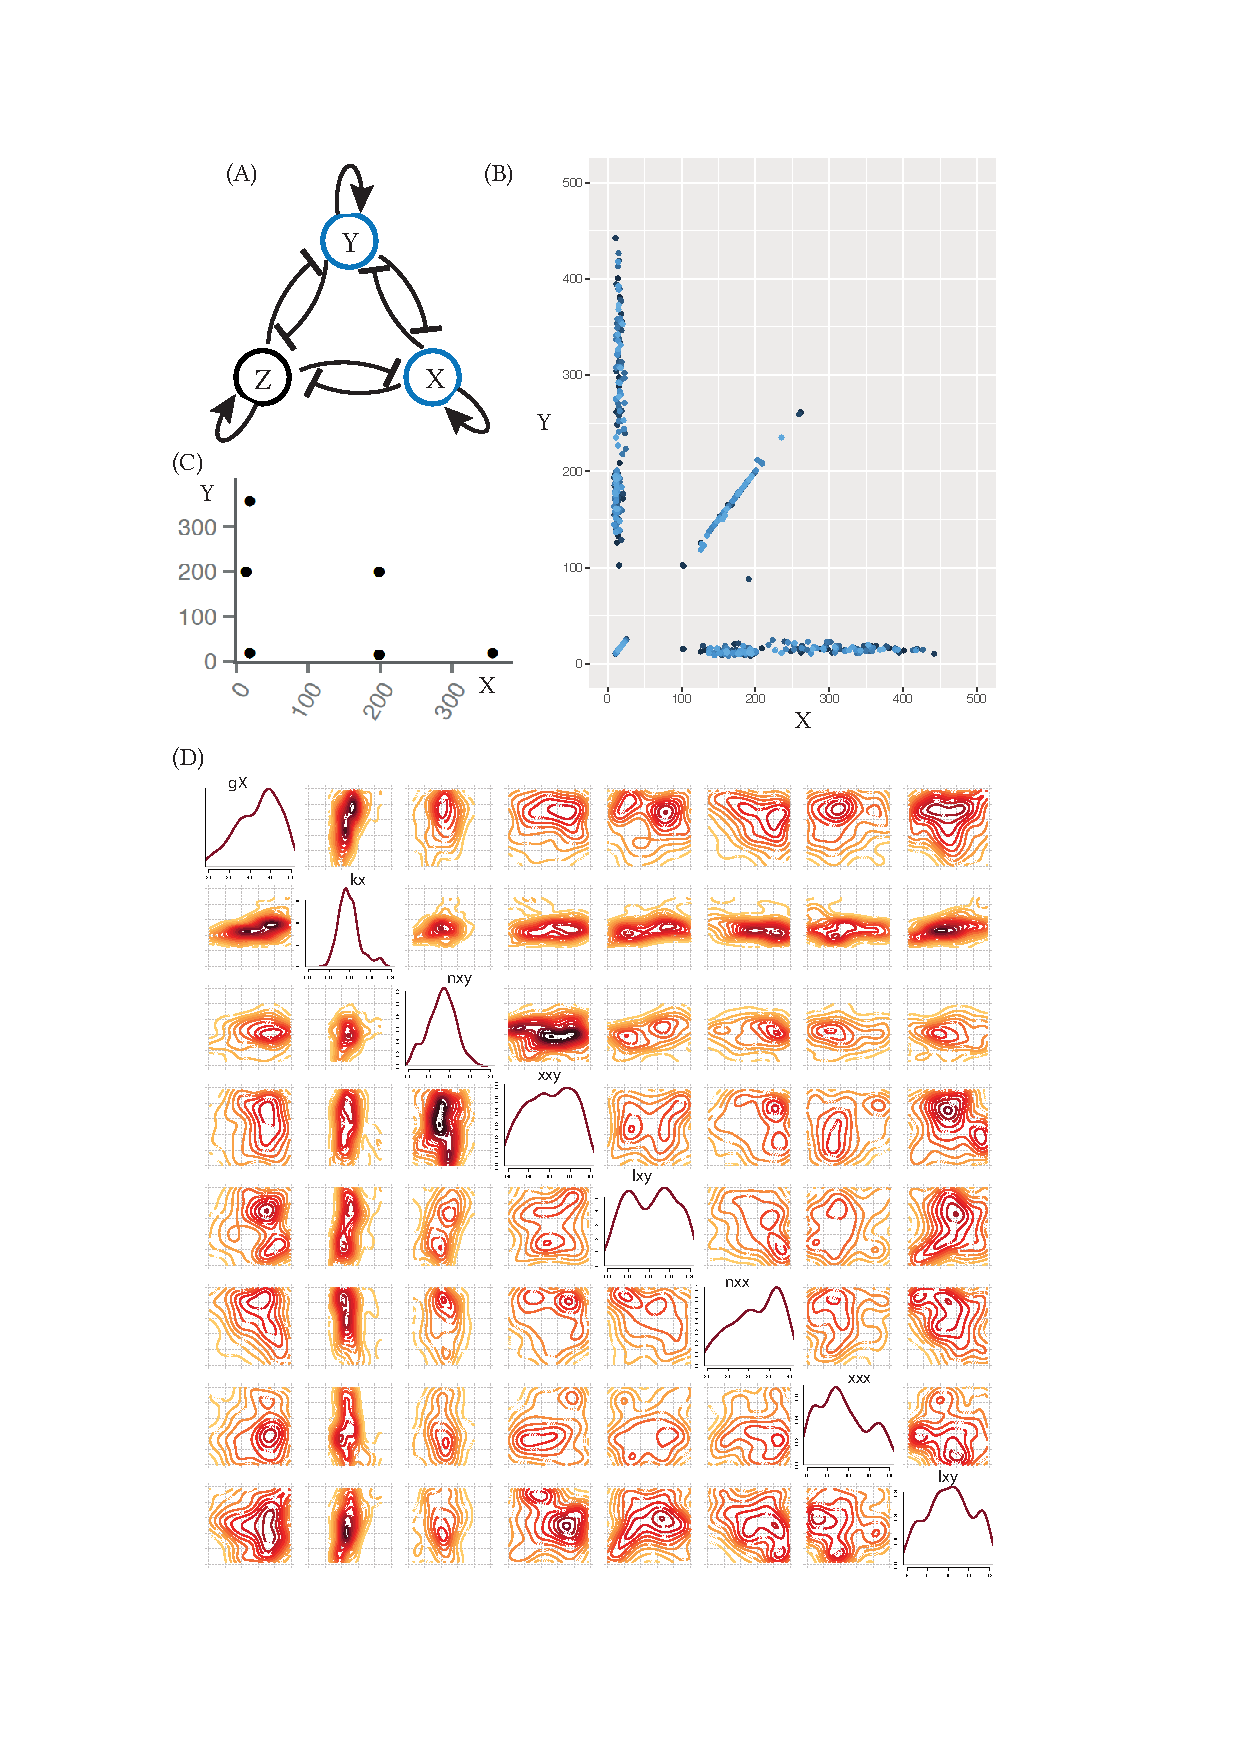
\includegraphics[scale=0.6]{../../chapters/chapterStabilityFinder/images/lu_6ss_w.pdf}
\caption[The three-node mutual repression model, with added positive auto-regulation on each node.]{ \label{fig:fig8}The three-node mutual repression model, with added positive auto-regulation on each node. (A) The model. The model is studied in two dimensions using StabilityFinder, for nodes $X$ and $Y$. (B) The phase plot of 100 particles from the posterior found by StabilityFinder. (C) An example phase plot from one particle. There are 6 steady states. (D) The posterior distribution of the 6-steady state three-node system. Parameters $kx$ and $nxy$ are the most constrained.}
\end{center}
\end{figure*}


We find that the most constrained parameters for this behaviour are again the degradation rate of the proteins, $kx$. If they are too large or too small the system will not exhibit hexa-stability. Additionally we find that the Hill coefficients for the repressors, $nxy$, are constrained to be smaller than 1.5 as seen in Figure~\ref{fig:fig8}D. 

Consistently with the results found in Section~\ref{sec:lu_234}, we find that the steady states are symmetric (Figure~\ref{fig:fig8}B). Each of six steady states exists in symmetry with another one, in tightly constrained regions. This example demonstrates that StabilityFinder can be used to elucidate the dynamics of more complex network architectures, which will be key to the successful design and construction of novel gene networks as synthetic biology advances.


\clearpage
\subsection{StabilityFinder used on the more general mass action switches}
\label{sec:ma_sw}						
%Although the DP switch can achieve tristability, we investigated how the addition of positive autoregulation alters the robustness of the switch for bistable behaviour. Here we define a robust system as a device that can withstand fluctuations in parameter values and still produce the desired behaviour (parametric robustness). Feedback loops are well known key regulatory motifs~\autocite{Brandman:2005ci}. Although negative feedback loops are essential for homeostasis and buffering~\autocite{Thomas:1995id} and can increase robustness to extrinsic noise sources, we focussed on the addition of positive feedback because this has been shown to increase robustness in other systems \autocite{XXX}. We use StabilityFinder to compare the two models, and determine whether its worthwhile building a bistable circuit with added positive feedback.
%StabilityFinder allows us to study more complex systems and to take stochasticity into account. This is relevant in a biological systems in which realistic models tend to involve many species and interactions and where small molecule numbers and external noise are non negligible. 

In order to study the switch system in a more realistic way, I developed an extension to the switches used in Sections~\ref{sec:gard} and~\ref{sec:lu}. This new set of switches does not use the \acrfull{qssa} that is often used in modelling the toggle switch. Using mass action, this changes the two-equation system used in~\textcite{Gardner:2000vha} and~\textcite{Lu:2014kc} into a system of 8 \acrshort{ode}s and 10 parameters in the classical switch case with no autoregulation (model \acrshort{cs-ma}). The equations describing the system are shown below. 
$$
\begin{array}{cccc}
      \textrm{gA}\stackrel{\textrm{geA}}{\longrightarrow}\textrm{gA} + \textrm{A} \\
      \textrm{gB}\stackrel{\textrm{geB}}{\longrightarrow}\textrm{gB} + \textrm{B} \\
      \textrm{A} + \textrm{A} \stackrel{\textrm{dim}}{\longrightarrow}\textrm{A2} \\
      \textrm{A2} \stackrel{\textrm{dim r}}{\longrightarrow}\textrm{A} + \textrm{A} \\
      \textrm{B} + \textrm{B} \stackrel{\textrm{dim}}{\longrightarrow} \textrm{B2} \\
      \textrm{B2} \stackrel{\textrm{dim\_r}}{\longrightarrow}\textrm{B} + \textrm{B} \\
      \textrm{gA} + \textrm{B2} \stackrel{\textrm{repA}}{\longrightarrow}\textrm{B2gA} \\
      \textrm{B2gA} \stackrel{\textrm{rep\_r}}{\longrightarrow}\textrm{B} + \textrm{gA} \\
      \textrm{gB} + \textrm{A2} \stackrel{\textrm{repB}}{\longrightarrow}\textrm{A2gB} \\
      \textrm{A2gB} \stackrel{\textrm{rep\_r}}{\longrightarrow}\textrm{A2} + \textrm{gB} \\
      \textrm{A} \stackrel{\textrm{deg}}{\longrightarrow}\varnothing\\
      \textrm{A2} \stackrel{\textrm{deg\_dim}}{\longrightarrow} \varnothing\\
      \textrm{B2} \stackrel{\textrm{deg\_dim}}{\longrightarrow}\varnothing\\
\end{array}
$$

\noindent For the model with added double positive autoregulation (model \acrshort{dp-ma}) the following equations are added to the system: 

$$
\begin{array}{cccc} 
    \textrm{A2} + \textrm{gA} \stackrel{\textrm{aut\_1}}{\longrightarrow} \textrm{A2gA} \\
    \textrm{A2gA} \stackrel{\textrm{aut\_2}}{\longrightarrow} \textrm{A} + \textrm{A2gA}\\
    \textrm{A2gA} \stackrel{\textrm{aut\_3}}{\longrightarrow} \textrm{A2}+ \textrm{gA}  \\
    \textrm{B2} + \textrm{gB} \stackrel{\textrm{aut\_1}}{\longrightarrow} \textrm{B2gB} \\
    \textrm{B2gB} \stackrel{\textrm{aut\_2}}{\longrightarrow} \textrm{B} + \textrm{B2gB}\\
    \textrm{B2gB} \stackrel{\textrm{aut\_3}}{\longrightarrow} \textrm{B2}+ \textrm{gB}  \\
\end{array}
$$

\noindent The \acrshort{ode}s describing the above switches are shown in Appendix~\ref{ap:ODEs}. These models are too complex to be solved analytically and I use StabilityFinder to fit the models to a bistable behaviour using the prior distributions shown in Table~\ref{tab:MA_priors}. The prior values were chosen using the parameter scan used in Chapter~\ref{ch:abcsysbio}. All priors given assume a uniform distribution. The two models used and the resulting phase plots are shown in Figure~\ref{fig:ma-cs-dp-phase} and the posterior distributions obtained are shown in Figure~\ref{fig:ma-sym-det-post}. 


\begin{table}[htpb]
\centering
\caption{The priors used in the classic (CS) and double positive (DP) mass action deterministic and stochastic models }
\label{tab:MA_priors}
\rotatebox{90}{
\begin{tabular}{@{}llllllll@{}}
\toprule
\multicolumn{1}{c}{\multirow{4}{*}{Description}} & \multicolumn{1}{c}{\multirow{4}{*}{Parameter}} & \multicolumn{6}{c}{Models} \\ \cmidrule(l){3-8} 
\multicolumn{1}{c}{} & \multicolumn{1}{c}{} & \multicolumn{2}{c}{Deterministic} & \multicolumn{4}{c}{Stochastic} \\ \cmidrule(l){3-8} 
\multicolumn{1}{c}{} & \multicolumn{1}{c}{} & \multicolumn{1}{c}{\multirow{2}{*}{CS}} & \multicolumn{1}{c}{\multirow{2}{*}{DP}} & \multicolumn{2}{c}{CS} & \multicolumn{2}{c}{DP} \\ \cmidrule(l){5-8} 
\multicolumn{1}{c}{} & \multicolumn{1}{c}{} & \multicolumn{1}{c}{} & \multicolumn{1}{c}{} & \multicolumn{1}{c}{Bistable} & \multicolumn{1}{c}{Tristable} & \multicolumn{1}{c}{Bistable} & \multicolumn{1}{c}{Tristable} \\ \midrule
Gene expression & geA, B & 5-10 & 1-10 & 0-10 & 0-10 & 0-10 & 0-10 \\
Dimerization & dim & 5-10 & 1-10 & 7-15 & 0-3 & 7-15 & 0-3 \\
Monomerization & dim\_r & 0-5 & 0-5 & 0-10 & 0-10 & 0-10 & 0-10 \\
Repression & repA, B & 2-10 & 1-10 & 0-10 & 0-10 & 0-10 & 0-10 \\
Dissociation of repressor & rep\_r & 0-5 & 1-10 & 0-10 & 0-10 & 0-10 & 0-10 \\
Protein degradation & deg & 1-5 & 0-10 & 0-10 & 0-10 & 0-10 & 0-10 \\
Dimer degradation & deg\_dim & 0-0.1 & 0-0.5 & 0-1 & 0-1 & 0-1 & 0-1 \\
Dimer promoter self-association & aut\_1 &  & 1-10 &  &  & 0-10 & 0-10 \\
Dimer promoter self-activation & aut\_2 &  & 5-10 &  &  & 0-10 & 0-10 \\
Dimer promoter self-dissociation & aut \_3 &  & 1-5 &  &  & 0-10 & 0-10 \\ \bottomrule
\end{tabular}
}
\end{table}

\begin{figure*}[htbp]
\begin{center}
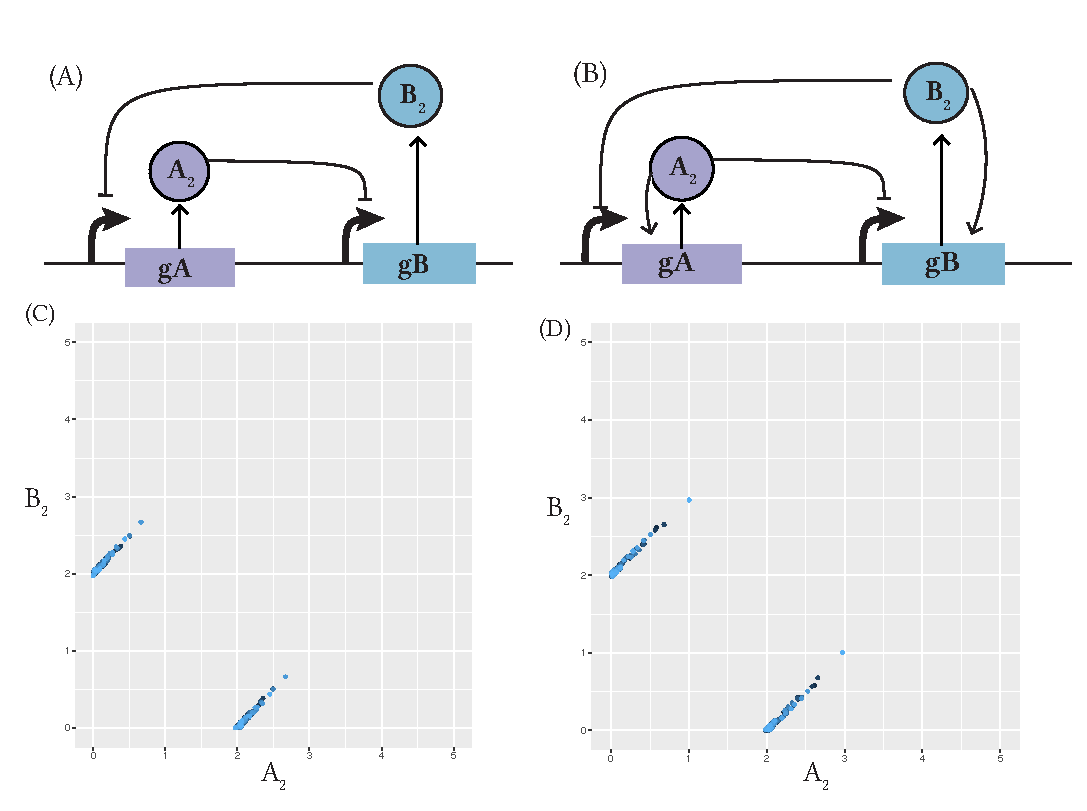
\includegraphics[scale=0.7]{../../chapters/chapterStabilityFinder/images/MA-cs-dp-phase.png}
\caption[The mass action toggle switches and phase plots]{ \label{fig:ma-cs-dp-phase} Illustrations of the two mass action switches I developed. (A) The simple switch \acrshort{cs-ma} (B) The switch with double positive autoregulation \acrshort{dp-ma}. (C, D) The phase plots of 100 particles simulated from the posterior distributions of the bistable mass action switches.}
\end{center}
\end{figure*}


\begin{figure*}[htbp]
\centerfloat
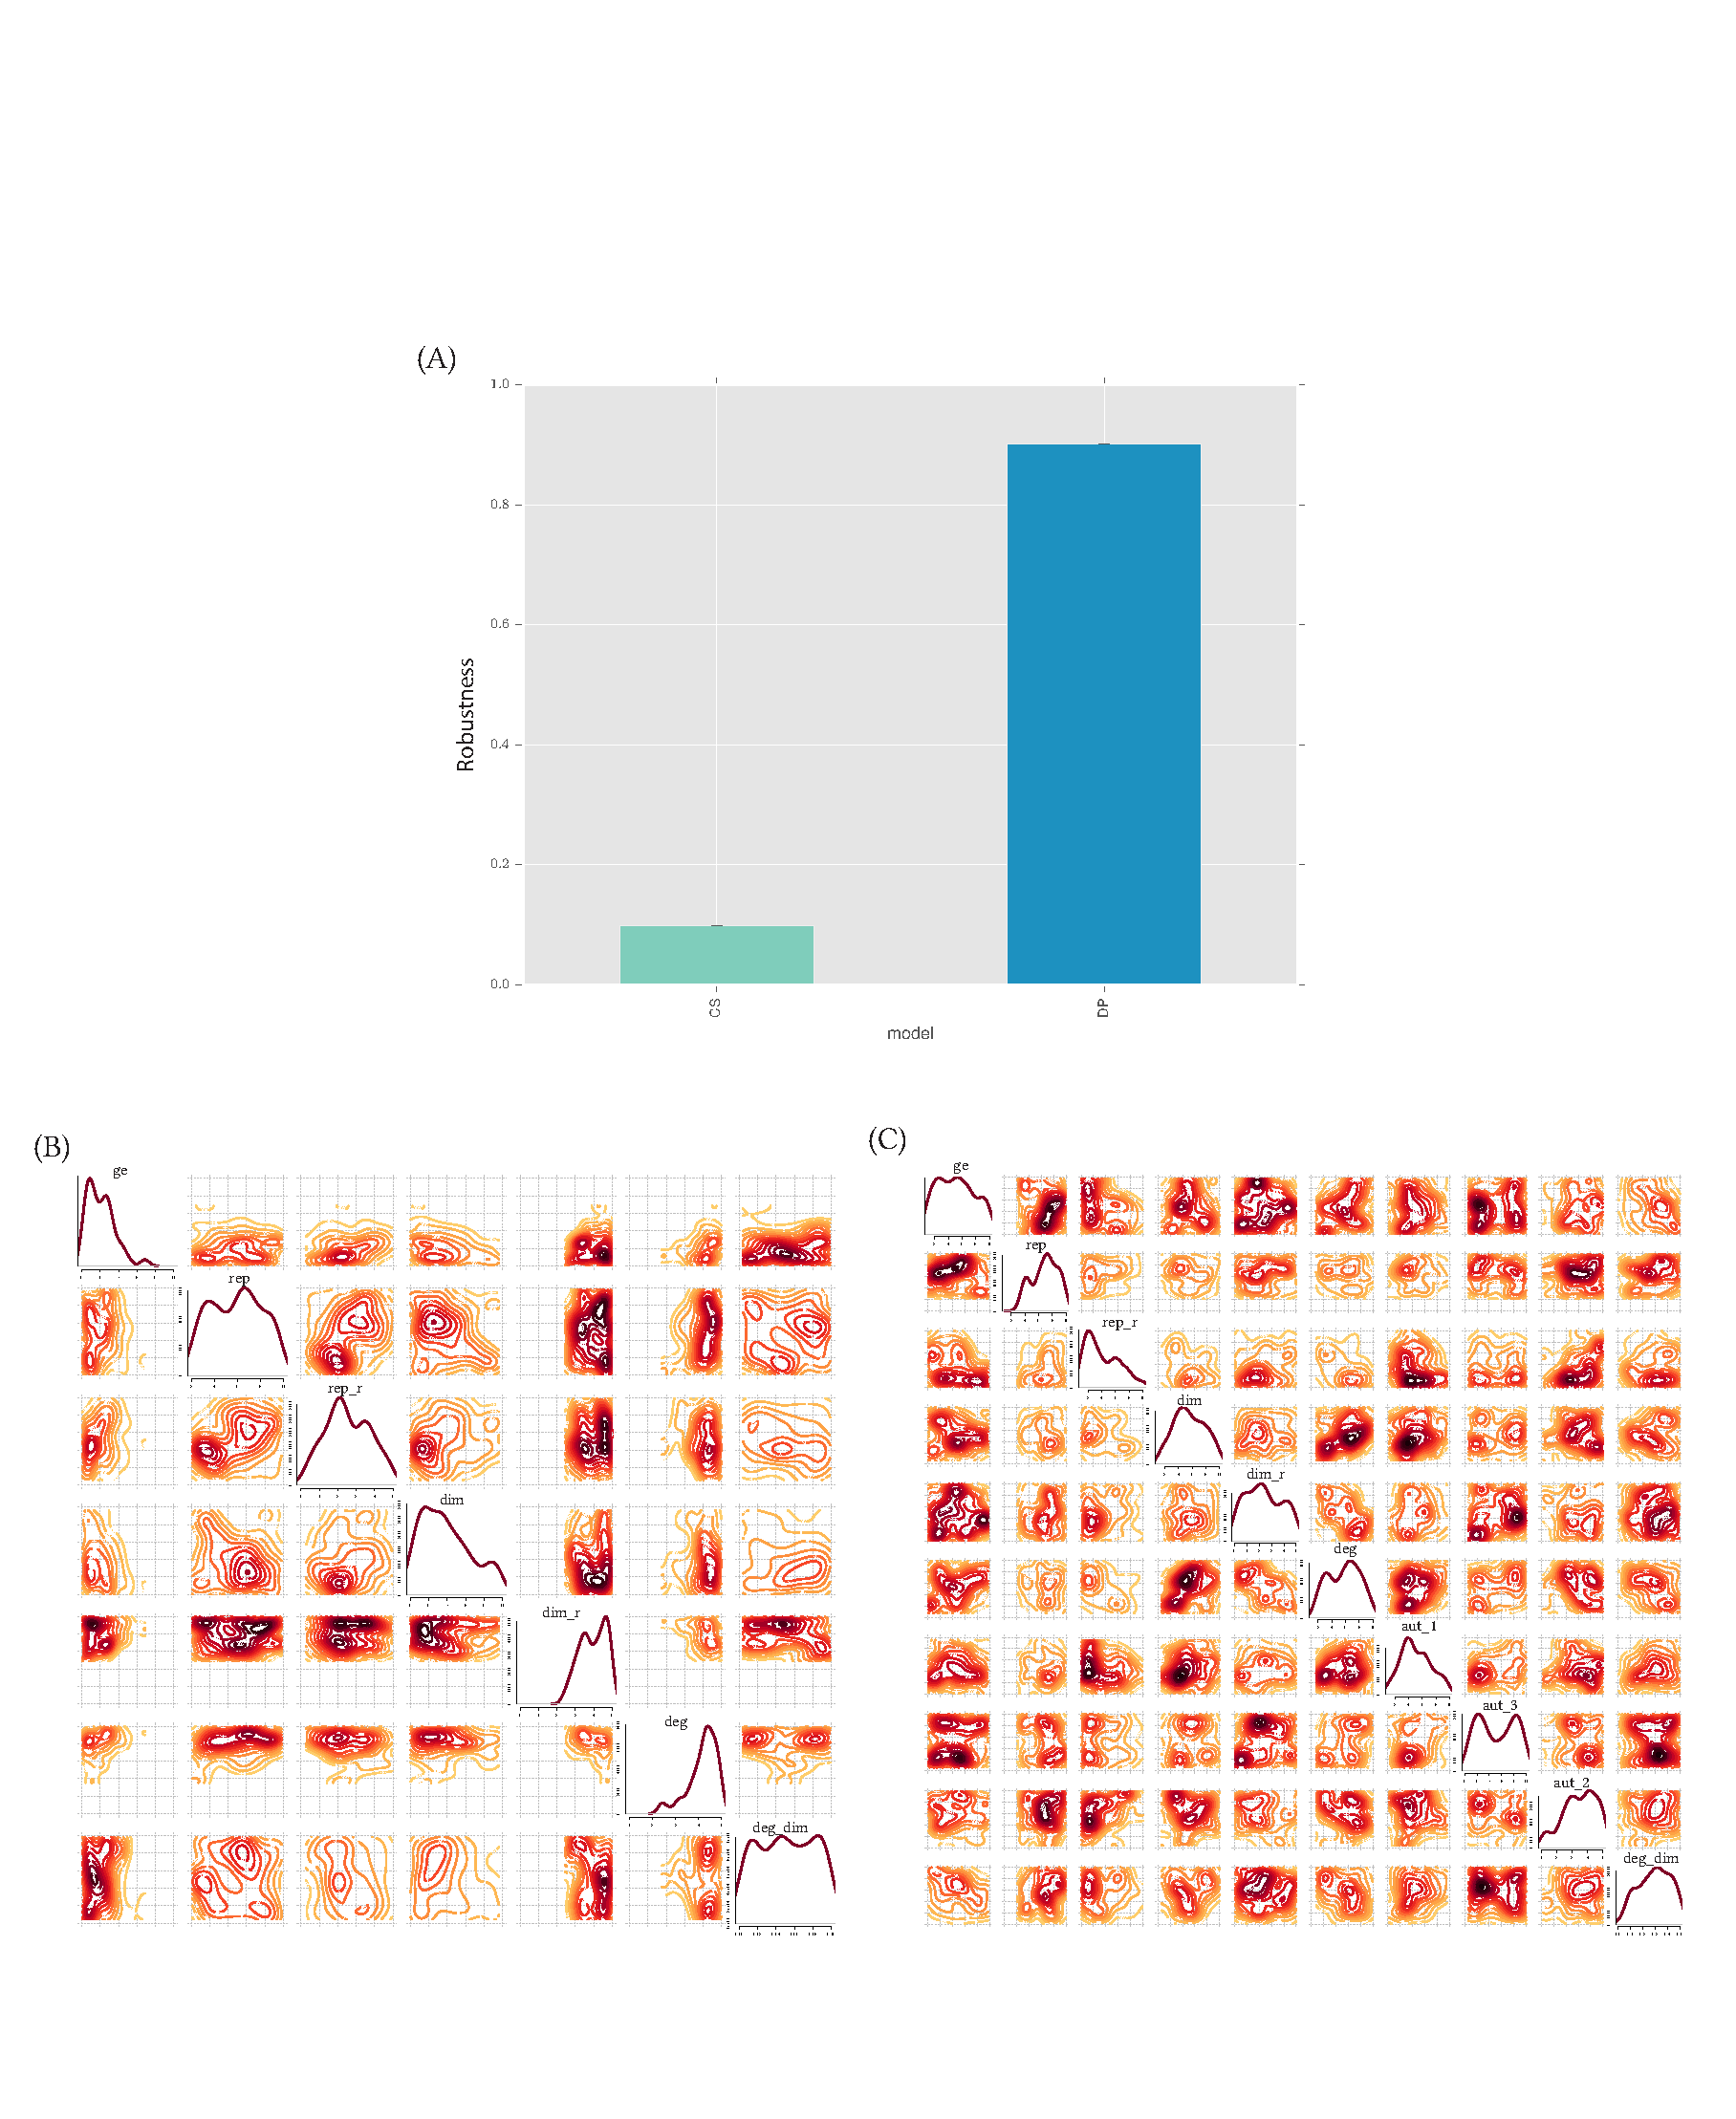
\includegraphics[width=1.1\textwidth]{../../chapters/chapterStabilityFinder/images/MA_sym_post_w.pdf}
\caption[Robustness comparison of the \acrshort{cs-ma} and \acrshort{dp-ma} switches]{ \label{fig:ma-sym-det-post}(A) Robustness comparison of the \acrshort{cs-ma} and \acrshort{dp-ma} switches. The Bayes factor of $\frac{p(B|CS)}{p(B|DP)}$ was found to be 9.14. The posterior distributions of (B) \acrshort{cs-ma} and (C) \acrshort{dp-ma} switches. }
\end{figure*}


By examining the posterior distributions shown in Figure~\ref{fig:ma-sym-det-post} we see that the \acrshort{cs-ma} is much more constrained that the \acrshort{dp-ma} switch. We find that gene expression must be low for bistability to occur in the \acrshort{cs-ma} model but there is no such constraint in the \acrshort{dp-ma} model. We also find that the monomerization rate $dim\_r$ and the monomer degradation rate $deg$ must both be larger than 2. This is not found in the \acrshort{dp-ma} model. 

Next I compare the two models for robustness using the ellipsoid method described in Section~\ref{sec:cal_rob}. We find that the addition of positive feedback loops greatly increases the system's robustness to parameter fluctuations as seen in Figure~\ref{fig:ma-sym-det-post}A, The Bayes factor of $\frac{p(B|CS)}{p(B|DP)}$, where $B$ is bistable behaviour, was found to be 9.14. Adding positive feedback loops to the model allows it to be bistable over a greater range of parameter values. This indicates that small fluctuations in parameters in the cellular environment will not revert it to monostability and thus makes it more suitable for use in synthetic biological applications where inconsistent stability profile of a system could be detrimental. This makes it a better candidate for building new synthetic devices based on the toggle switch design. We identified the parameter region within which these models are bistable, information that is important when building such a device in the lab.

The models used in the above analysis assume the parameters for equivalent reactions are equal. This is a constraint that simplifies the model. When building this model into a synthetic system in the lab, this assumption is not necessarily justified. When choosing promoters to build this synthetic system two promoters can be chosen to have similar strength but their strength will not necessarily be identical.  In order to study how this might affect the results, I further eliminate modelling assumptions made in the toggle switch by making the parameters representing gene expression ($ge$) and repression ($rep$), as well as the protein degradation parameters asymmetric (independent parameters for each protein, versus fixed to be equal). We find that the features of the posterior distributions of the symmetric and the asymmetric models remain the same. The reader is referred to Appendix~\ref{ap:figures} for the posterior distributions of the asymmetric models. 

%The posterior distribution of the asymmetric \acrshort{cs-ma} model was more constrained than the posterior distribution of the asymmetric \acrshort{dp-ma} model. 

I further study the asymmetric mass action models by examining the \acrshort{qssa}. As stated in Section~\ref{sec:qssa}, the \acrshort{qssa} is a common analytical tool for model simplification. By examining the posterior distributions of the \acrshort{cs-ma} we can determine whether the \acrshort{qssa} is justified in these models. As stated in Section~\ref{sec:qssa}, the assumption that has to be made for the \acrshort{qssa} to hold is that the rate of binding and unbinding of the transcription factors to the promoters is very fast. The rates have to be much faster than the rates of their production and decay in the system in order to justify that the reaction take place in separate time scales and can thus be assumed to always be at steady state. The \acrshort{qssa} is also made for the dimerization of the transcription factors. Therefore, for the \acrshort{qssa} to be justified in the toggle switch, the rates for association ($rep$) and dissociation ($rep\_r$) of the transcription factors to the promoters, as well as the rates for dimerization ($dim$) and monomerization ($dim\_r$) of the transcription factors have to be much larger than any other rate.


In order to determine whether this is the case here, I plot the marginal distributions of each of the parameters assumed to be very large ($rep$, $rep\_r$, $dim$, $dim\_r$) against each of the parameters involved in the expression and decay of the proteins. This is shown in Figure~\ref{fig:ma_qssa}. We find that the \acrshort{qssa} can be justified only with respect to the rate of degradation of the transcription factor dimers ($deg\_dim$). All parameters under consideration for the \acrshort{qssa} ($rep$, $rep\_r$, $dim$, $dim\_r$) are found to be much larger than $deg\_dim$. On the other hand, the \acrshort{qssa} cannot be justified with respect to gene expression ($ge$) or protein degradation ($deg$). It is seen in Figure~\ref{fig:ma_qssa} that the rates under consideration for the \acrshort{qssa} are not much larger than the rates of protein production and decay, and thus it cannot be assumed that they are always at steady state. This means that the CS-MA model functions as a switch even when the \acrshort{qssa} does not hold. These assumptions, necessary for the reduction of the model, are therefore not always justified in real systems. 

% If $rep$, $rep_r$, $dim$ and $dim_r$ are much larger than the rates for production and decay of the proteins, the distribution will be  




\begin{figure*}[htbp]
\begin{center}
\includegraphics[width=\textwidth]{../../chapters/chapterStabilityFinder/images/qssa-cs-sym.png}
\caption[Testing the QSSA assumptions on the mass action models]{ \label{fig:ma_qssa}The \acrshort{qssa} cannot be justified for the CS-MA model. The dotted line denotes the line where $x = y$. The posterior distributions of the rates under consideration, $rep$, $rep\_r$, $dim$, $dim\_r$, are all much larger than the rate of degradation of the transcription factor dimer. (A) The rate of binding of the repressors to the promoter is not much larger than the rate of protein expression and degradation. (B) The rate of protein expression and decay are both larger than the rate of dissociation of the dimer to the promoter. (C) The rate of transcription factor dimerization is larger than the rates of protein production and decay, but not by a big amount. (D) The rate of monomerization of the transcription factors is smaller than the rates of protein expression and decay.}
\end{center}
\end{figure*}
\clearpage


%I further investigated modelling assumptions by separating transcription and translation into two separate steps. This makes the models more realistic but also more complex and StabilityFinder is ideal for analysing them.  It is known that transcription in prokaryotes occurs in bursts~\cite{Golding:2005uv} so an interesting question is whether transcriptional bursting has an effect on bistability. To investigate this I added a multiplicative term to the \acrshort{ode}s for mRNA production. Using StabilityFinder on these models we find that transcriptional bursting does not affect a system's ability to be bistable. 

\subsubsection{Multistability in the stochastic mass action switches}

To investigate how the level of abstraction affects switch design principles, I expand the analysis under the assumption of mass action kinetics and stochastic dynamics. The asymmetric \acrshort{cs-ma} and \acrshort{dp-ma} models are simulated using the Gillespie algorithm~\autocite{Gillespie:1977ww}. The priors used are given in Table~\ref{tab:MA_priors}.

\textcite{Ma:2012dt} found that the stochastic fluctuations in a system involving such a small number of molecules, like the toggle switch, uncovers effects that can not be predicted by the fully deterministic case~\autocite{Ma:2012dt}. We find that in the stochastic case, both the simple switch, \acrshort{cs-ma} , and positive autoregulation switch, \acrshort{dp-ma}, are capable of both bistable and tristable behaviour. The fact that tristability can occur in the classical model is consistent with the effect of small molecule numbers; if gene expression remains low, it provides the opportunity for small number effects to be observed, and the third steady state to stabilise \autocite{Ma:2012dt}. In order to ensure that the tristable switches found in the stochastic case are truly tristable, I re-sample the posterior distributions and simulate to steady state. If the resulting phase plots are tristable then we know that the posterior truly represents tristability. 


\begin{table}[tb]
\centering
\caption{Design principles of the stochastic MA bistable and tristable switches}
\label{tab:des_prin}
\begin{tabular}{@{}ccccc@{}}
\toprule
                    & \multicolumn{2}{c}{\textbf{\acrshort{cs-ma}}} & \multicolumn{2}{c}{\textbf{\acrshort{dp-ma}}} \\ \cmidrule(l){2-3}\cmidrule(l){4-5}
                    & \textit{Bistable}    & \textit{Tristable}   & \textit{Bistable}    & \textit{Tristable}   \\\cmidrule(l){2-2}\cmidrule(l){3-3}\cmidrule(l){4-4}\cmidrule(l){5-5}
dimerisation        & High        & Low         & High        & Low         \\
protein degradation & -           & -           & -           & Low         \\
dimer degradation   & Low         & -           & Low         & -           \\\bottomrule
\end{tabular}
\end{table}

As can be seen in Figure~\ref{fig:fig7}, differences in the parameter values are observed between the bistable and tristable switches, in both \acrshort{cs-ma} and \acrshort{dp-ma} models. We find that the simple switch is tristable when dimerisation rate is low and bistable when it is high. The degradation of the dimer proteins must have a low rate for bistability but there are no restraints in the case of the tristable switch. For the case of the DP switch, we find that the rates for dimerisation, degradation and dimer degradation are different for the bistable and tristable behaviours (Figure~\ref{fig:fig7}). The rate of dimerisation must be low for tristability to occur and large for bistability, as observed for the simple switch. The parameter for protein degradation must be low for tristability whereas there are no constraints for the bistable case. Finally, the parameter for dimer degradation must be low for bistability whereas it has no constraints for tristability, as observed in the simple switch. The design principles for both the \acrshort{cs-ma} model and the \acrshort{dp-ma} model are summarised in Table~\ref{tab:des_prin}



\begin{figure*}[htbp]
\centerfloat
\includegraphics[width=1.1\textwidth]{../../chapters/chapterStabilityFinder/images/MA_stoch_design_princ.png}
\caption[Multistability in the stochastic mass action models]{ \label{fig:fig7}: Tristability is possible in the mass action toggle switch models when simulated stochastically. (A) The simple toggle switch with no autoregulation can be both bistable and tristable. The two posteriors are shown, where the posterior distribution of the bistable switch is shown in blue and of the tristable switch in red. From the posterior distribution we can deduce the the dimerization parameter must be small for tristability to occur but large for bistability. The switch with double positive autoregulation and its posterior distributions for the bistable and tristable case are shown in (B). (C) A sample phase plot of a stochastic tristable and bistable mass action switch. }
\end{figure*}
\clearpage


\subsubsection{Bayes factors depend on the choice of priors}

An important aspect of Bayes factors, and thus robustness, that must be investigated is its dependence on the prior distributions. From Equation~\ref{eq:final_bayes} we can expect that the measure for robustness will depend on the size of the prior. The prior distributions for model comparison are ideally chosen by using related data that can inform the choice. But this situation can be rare and priors are selected by using information from the literature in combination with rough guesses~\autocite{Kass:1995vb}. Often simplifications are made and the choice of large prior ranges can seem like like an attractive option, as to impose less bias to the priors. Nevertheless this can have an effect on the Bayes factors calculated. The choice of improper, or very large priors can skew Equation~\ref{eq:final_bayes} to favour one model over the other~\autocite{Kass:1995vb}. In this section I demonstrate that the choice of priors for the toggle switch models has a significant effect on the calculated robustness of the models. This has to be taken under consideration when analysing candidate models for use in synthetic biology applications, as a poor choice of priors can skew the robustness analysis in favour of one model over the other, when no such robustness gain will be observed \textit{in vivo}.    

In order to demonstrate the effect of prior choice on robustness, I use the \acrshort{cs-ma} model. I use StabilityFinder to approximate the posterior distribution that makes this model bistable using two ranges of prior distributions. The two sets of prior distributions used here are denoted as very narrow (VN2) and wide (W) in Table~\ref{tab:prior_study}. The posterior distributions obtained corresponding to the VN priors and W priors are shown in Figure~\ref{fig:priors_matter}A and B respectively. It can be seen that the posterior distribution of the model with VN2 priors is more constrained than the model with W priors. This indicates that if one of the parameters is able to have a larger value, then the constraints on the rest of the parameters are not necessary any more. This results in the unconstrained posterior distribution observed in Figure~\ref{fig:priors_matter}B.

\begin{table}[tb]
\centering
\caption{Priors used for studying the effect of priors to robustness}
\label{tab:prior_study}
\begin{tabular}{@{}cccc@{}}
\toprule
         & VN2 & N1  & W    \\ \midrule
ge       & 5 - 10      & 1 - 10  & 1 - 100 \\
rep      & 2 - 10      & 1 - 10  & 1 - 100 \\
rep\_r   & 0 - 5       & 1 - 10  & 0 - 10  \\
dim      & 5 - 10      & 1 - 10  & 0 - 10  \\
dim\_r   & 0 - 5       & 0 - 5   & 0 - 10  \\
deg      & 1 - 5       & 0 - 10  & 0 - 100 \\
deg\_dim & 0 - 0.1     & 0 - 0.5 & 0 - 1   \\ \bottomrule
\end{tabular}
\end{table}

Furthermore, I test the effect of the prior range to the robustness of the model for each parameter separately. For each test, the prior distributions of all the parameters correspond to the range given in column VN2 in Table~\ref{tab:prior_study} except for the parameter being tested. For each run one parameter is being tested and has a prior range equal to the range given in column W in Table~\ref{tab:prior_study}. StabilityFinder is then used to approximate the posterior distribution of the model, given the priors and bistable behaviour. Therefore, there are 7 posterior distributions of the bistable CS-MA switch, each one corresponding to one parameter having a wide prior range. For each run, the Bayes factor of the model compared to the \acrshort{dp-ma} model used in Figure~\ref{fig:ma-sym-det-post} is calculated, using Algorithm~\ref{alg:robustness}. The posterior distribution for \acrshort{dp-ma} remains the same every time. Figure~\ref{fig:priors_matter}C shows the Bayes factors calculated for the DP-MA model against each run of the \acrshort{cs-ma}. We can see from Figure~\ref{fig:priors_matter}C that when the priors for $ge$ are much larger, the Bayes factor increases. The evidence for choosing DP-MA over CS-MA changes from substantial to strong, as defined in Table~\ref{tab:BAYES_FACTS}, by using a larger prior for parameter $ge$. This change is attributed to the fact the $ge$ is constrained to be low. If the prior range is much larger, it is evident that the ratio of the volumes of the functional region to the prior will be much smaller for CS-MA. %On the other hand, the range of the prior of parameter $deg\_dim$ does not increase the Bayes factor in favour of model DP-MA. This is in agreement with~\textcite{Kass:1995eh}, who 
 

\begin{figure*}[h]
\centerfloat
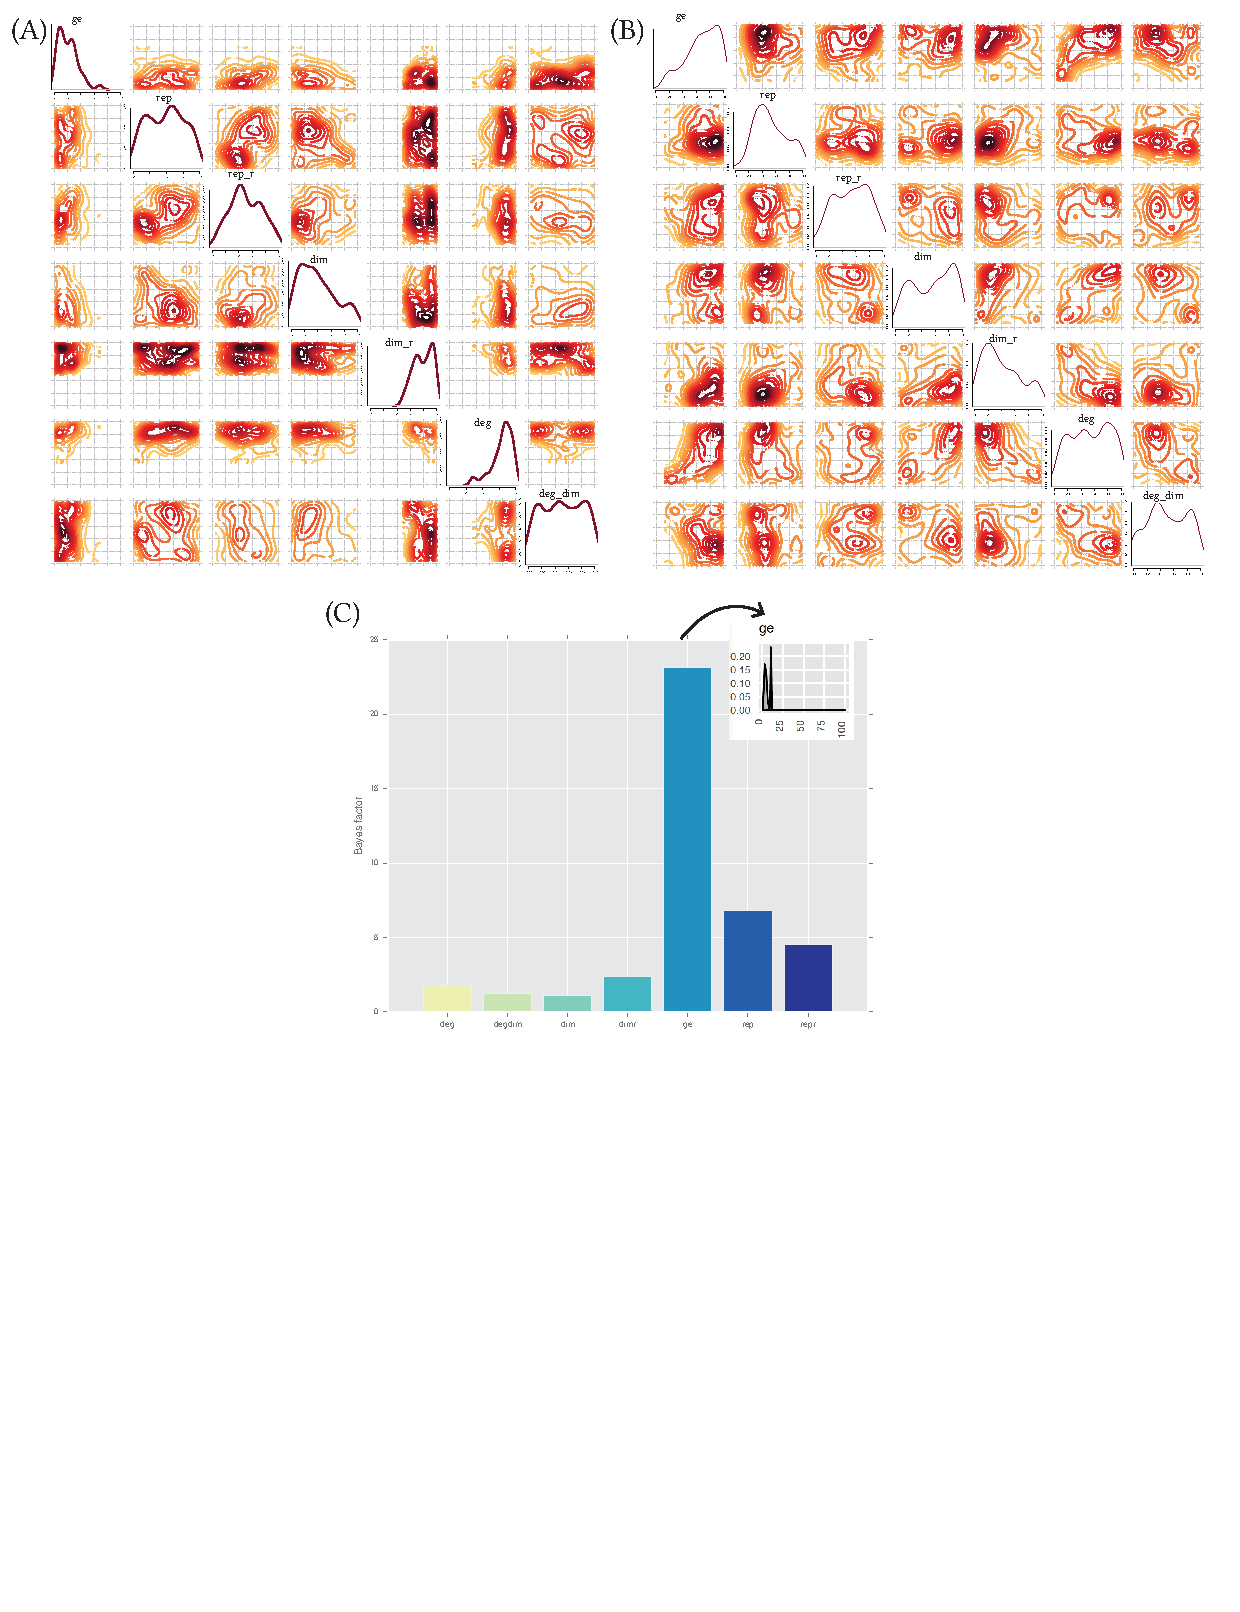
\includegraphics[width=1.2\textwidth]{../../chapters/chapterStabilityFinder/images/priors_matter_w.pdf}
\caption[The volume of the priors has an effect on the posterior distribution obtained.]{ \label{fig:priors_matter}The volume of the priors has an effect on the posterior distribution obtained. (A) The \acrshort{cs-ma} model with VN2 priors and (B) the \acrshort{cs-ma} with W priors. (C) The increase in robustness seen is due to the gene expression parameter prior being wide while the functional region remains constrained.}

\end{figure*}



In Section~\ref{sec:ma_sw} we found that the \acrshort{dp-ma} is more robust than the \acrshort{cs-ma} model. Here I want to test whether this result still remains when the priors of the models are made wider. In order to test that, I change the prior ranges of both models and measure their robustness each time using Algorithm~\ref{alg:robustness}. The classes of priors used are given in Table~\ref{tab:prior_study}. The robustness measures calculated, which corresponds to the fraction of the volume of the functional region over the volume of the prior, are shown in Figure~\ref{fig:priors_matter2}A. 

%The Bayes factors, corresponding to the ratio of the robustness measure of \acrshort{dp-ma} to the robustness measure of \acrshort{cs-ma} is given relative to the difference in the volumes of the priors of the two models in Figure~\ref{fig:priors_matter2}B.

We find that the robustness measure changed as the priors of the models changed. When both models have very narrow or when both models have wide priors then their robustness measures are very similar. When both models have vary narrow priors the Bayes factor is equal to 1.32 and when the priors are wide the Bayes factor is equal to 1.06. In both these cases the Bayes factor is less than 3.2, and therefore is considered not significant~\autocite{Kass:1995vb}. When the priors for both models are narrow, the Bayes factor is equal to 2.25, which is still considered not significant. Most notably, when the priors for the \acrshort{cs-ma} model are very narrow and the priors of the \acrshort{dp-ma} model are narrow, the Bayes' factor is at 9.14. The Bayes factor is now greater than 3.2, but less than 10, and is thus considered substantial~\autocite{Kass:1995vb}.  These results are summarised in Table~\ref{tab:bayes_vols}.

\begin{table}[tb]
\centering
\caption{Bayes factors of the \acrshort{dp-ma} against the \acrshort{cs-ma}  model using different volumes of priors}
\label{tab:bayes_vols}
\begin{tabular}{@{}ccc@{}}
\toprule
\multicolumn{2}{l}{Prior volume} & \multirow{2}{4cm}{Bayes factor  ($\frac{p(B|DP-MA}{p(B|CS-MA)}$)  } \\ \cmidrule(r){1-2}
\acrshort{cs-ma}  & \acrshort{dp-ma} &  \\ \midrule
VN2 & VN2 & 1.32 \\
VN2 & N1 & 9.14 \\
N1 & N1 & 2.25 \\
W & W & 1.06 \\ \bottomrule
\end{tabular}
\end{table}

It is evident that the robustness measure depends on the prior volume. It is therefore useful to think of the Bayes factor in terms of the difference in the volume of the priors of the models that are being compared. I carry out this analysis for the above priors and the results are shown in Figure~\ref{fig:priors_matter2}B. Here we see that even though the prior difference is within the same order of magnitude, the Bayes factor increases significantly. This point corresponds to the case where the priors of \acrshort{cs-ma} are very narrow and the priors of \acrshort{dp-ma} are narrow, and that is where we see the Bayes factor between the two models is maximised. %We can take advantage of this observation to design a switch with double positive autoregulation that is significantly more robust than the Gardner toggle switch. By choosing the parameter values carefully we can maximise the gain of robustness that adding two positive feedback loops gives. 

\begin{figure*}[h]
\begin{center}
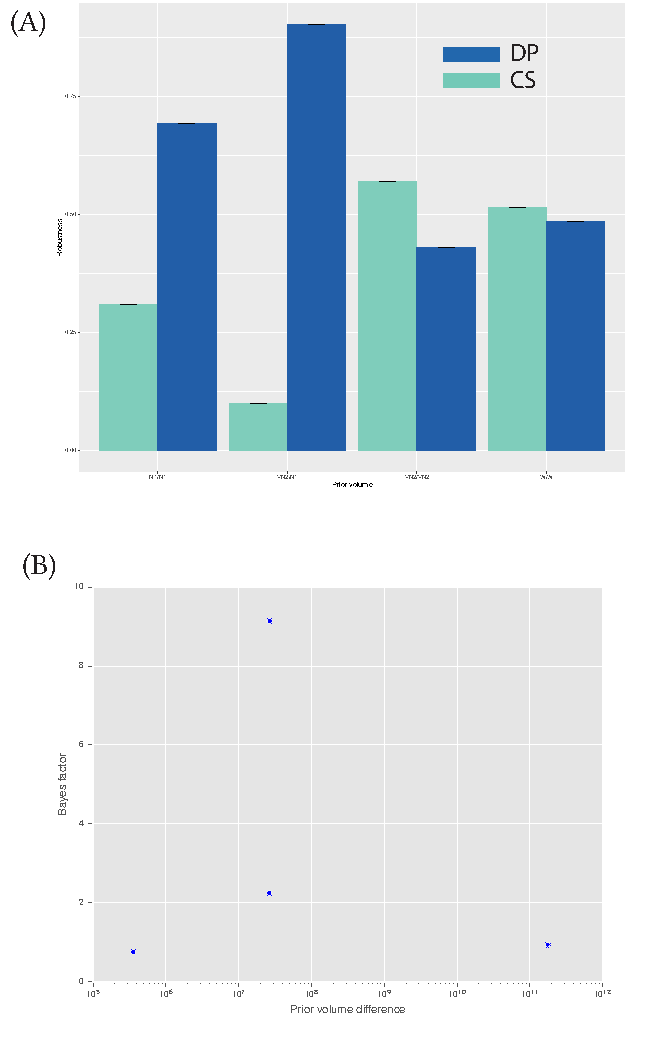
\includegraphics[scale=0.7]{../../chapters/chapterStabilityFinder/images/priors_matter_2.png}
\caption[Changing the priors in both models affects the robustness measure.]{ \label{fig:priors_matter2} Changing the priors in both models affects the robustness measure. (A) Using different prior ranges for the \acrshort{cs-ma} and the \acrshort{dp-ma} models yields different robustness for each. (B) The Bayes factor as a function of the prior volume difference. }
\end{center}
\end{figure*}

These results highlight the importance of choosing the ranges of priors for the models under consideration carefully. A balance has to be struck between restricting the prior ranges too much, where interesting behaviour in the model can be missed, and making the prior range too wide, where it becomes uninformative. 

\clearpage
%This indicates that small fluctuations in parameters in the cellular environment will not affect the system's ability to be bistable, and thus makes it more suitable for use in synthetic biological applications where a very constrained parameter set can be too restrictive.% This makes it a better candidate for building new synthetic devices based on the toggle switch design.

%We identified the parameter region within which these models are bistable, information that is important when building such a device in the lab. In the future, by selecting the system components accordingly, the parameter values can be adjusted \textit{in vivo}. For example, the desired level of gene expression can be accomplished by selecting the appropriate RBS sequence~\autocite{Salis:2009gk}. Another method to modify the parameter values \textit{in vivo} is to select the promoter to have the strength corresponding to the levels of gene expression and repression desired. Activity of each promoter can be measured and standardised~\autocite{Kelly:2009bj} making this process possible. For a system requiring more than one promoter, these can be efficiently selected from a promoter library using a genetic algorithm~\autocite{Wu:2011bq}. These standardised interchangeable components with known sequence and activity~\autocite{Kelly:2009bj,Canton:2008fv} can be selected and used to construct a desired system and replicate the parameter values found using StabilityFinder.

\section{Discussion}
  
 %This is critical to the design of novel synthetic switches, where the stability of a system has to be well defined and predictable.
 
 Here I developed a novel framework, StabilityFinder, that can be used to infer parameter values that can produce a desired system multistable behaviour. The novelty in the framework I developed over existing methodology is that complex models can be analyzed assuming either deterministic or stochastic dynamics. I have used StabilityFinder to uncover the design principles of a bistable, a tristable and a quadristable switch. I found key parameters that are important in determining the number of steady states a system is capable of. This is important in the design of novel synthetic switches, where the genetic parts chosen, with their corresponding reaction rates can have an effect on the stability of the system. A bistable, a tristable or a quadristable switch could each be used for different functions within a synthetic system. 
  
   %This is especially true when multiple such systems are used together, and the success of the whole system depends on all the parts working as expected. 
   
Being able to \textit{in silico} determine the stability a given system will aid in the design of novel synthetic circuits. In the future, by selecting the system components accordingly during sequence design, the parameter values can be selected \textit{in vivo}. For example, the parameter value corresponding to the translation initiation rate can be chosen by selecting the appropriate RBS sequence which given a nucleotide sequence will produce the desired rate~\autocite{Holtz:2010bm}, a method developed by~\textcite{Salis:2009gk}. Another method to tweak the parameter values \textit{in vivo} is to select the promoter to have the strength corresponding to the levels of gene expression and repression desired. Activity of each promoter can be measured and standardised~\autocite{Kelly:2009bj} making this process possible. For a system requiring more than one promoter, these can be efficiently selected from a promoter library using a genetic algorithm created by~\textcite{Wu:2011bq}. These standardised interchangeable components with known sequence and activity constitute the ultimate goal of synthetic biology..

 Nevertheless, it is important to note that StabilityFinder predicts the stability of a system in isolation. Recent body of work has shown that modules like the one studied here are not independent of downstream processes~\autocite{DelVecchio:2008gy, Ventura:2010ew, Jiang:2011ch, Lyons:2014iq}.~\textcite{Lyons:2014iq} showed that adding a downstream load to the genetic toggle switch can render it monostable. In order for multi-module systems to be successful, the effect of downstream loads to the system under study will have to be considered. Therefore extrapolation of the conclusions of StabilityFinder for a given module would not be justified when the module is part of a larger system of modules working in tandem.        
    
 %THIS IS ALL WORD FOR WORD FROM BACKGROUND OF CHAPTER ABC-SYSBIO CHANGE ONE OF THEM ASAP
% Tools that can identify parameter regions that give rise to specific behaviours will be key for the success of synthetic biology. In the future, by selecting the system components accordingly, the parameter values can be adjusted \textit{in vivo}. For example, the desired level of gene expression can be accomplished by selecting the appropriate RBS sequence~\autocite{Salis:2009gk}. Another method to modify the parameter values \textit{in vivo} is to select the promoter to have the strength corresponding to the levels of gene expression and repression desired. Activity of each promoter can be measured and standardised~\autocite{Kelly:2009bj} making this process possible. For a system requiring more than one promoter, these can be efficiently selected from a promoter library using a genetic algorithm~\autocite{Wu:2011bq}. These standardised interchangeable components with known sequence and activity~\autocite{Kelly:2009bj,Canton:2008fv} can be selected and used to construct a desired system and replicate the parameter values found using StabilityFinder.

The methodology used here can only be used to study the presence of a given stability and not its absence. If the algorithm is not converging it cannot be concluded that the given model is not capable of the desired stability under these priors. For example, the mass action switches were found to be both bistable and tristable when stochastic effects were taken into account. Using deterministic dynamics the algorithm did not converge using priors within the ranges used in this work. Nevertheless this does not permit the conclusion of absence of tristability in the deterministic classic or double positive mass action switch models. StabilityFinder only permits the interpretation of models that have converged to a given stability. 




StabilityFinder can also be used to study the topology of more complex multistable switches that exist in natural biological systems such as developmental pathways. I limited this framework to the objective behaviour of a given number of stable steady states. This could be extended to examine systems with a given switching rate or systems robust to a particular set of perturbations, both of which could be of great importance for building more complex genetic circuits.

Importantly I find that the prior distributions used during such an analysis greatly affect the robustness observed. More generally, the assumptions made when building a model can have a significant effect on the predictions made. This is consistent with current understanding~\autocite{Babtie:2014jg} and highlights the importance of the combination of experimental work and systems modelling, in order to understand the rules of thumb for abstraction in model based design of synthetic biological systems.

\section{Summary}

In this chapter I discussed the algorithm I developed and demonstrated how it can identify the parameter regions necessary for a model to achieve a given number of stable steady states. I used it to uncover the underlying principles that govern the stability of a given switch. 

I first tested StabilityFinder on a known switch and then proceeded to apply it to more complex models. I uncovered the design principles that make the Lu switch bistable, tristable or quadristable. I extended the Lu models to a three-node switch and showed how it can achieve 6 steady states. 

Furthermore, I built two novel models of the toggle switch which do not use the \acrshort{qssa} and showed that the \acrshort{qssa} cannot be justified in these models. Using these models I studied the effect positive autoregulation has on the robustness of a model. I also studied the effect the priors have on the posteriors and on the robustness of a model. Finally, using stochastic modelling I showed that these switch models are capable of both bistable and tristable behaviour. In the next chapter I study the genetic toggle switch in the lab and fit the toggle switch models used here to experimental data. 





%\section{Methods}

 
 
\subsection{Calculating robustness}




%\section{Results}
\subsection{Testing StabilityFinder: The Gardner toggle switch}

This toggle switch model was developed by T.~S. Gardner~\autocite{Gardner:2000vha}. This model consists of two mutually repressing transcription factors and is defined by the following ODEs:

\begin{align}
\frac{du}{dt} &= \frac{a_1}{1+v^{\beta}} - u \label{eq:gard_1} \\
\frac{dv}{dt} &= \frac{a_2}{1+u^{\gamma }} - v\label{eq:gard_2}
\end{align}
Where $a_1$ and $a_2$ are the effective rates of synthesis of repressors 1 and 2 respectively. \textit{u} is the concentration of repressor 1 and \textit{v} the concentration of repressor 2. \textit{$\beta$} is the cooperativity of repression of promoter 1 and \textit{$\gamma$} of repressor 2. In their paper,  T.~S. Gardner~\autocite{Gardner:2000vha} state that there are two conditions for bistability of this toggle switch model. That $a_1$ and $a_2$ are balanced and that $\beta$ and $\gamma$ are \textgreater 1. In order to test our methodology, we used StabilityFinder to find the posterior distribution for which this model exhibits bistable behaviour. So setting the desired behaviour to bistable, and using for priors a wide range of values that includes the values used in the Gardner paper, we test StabilityFinder to see if it finds the same conditions as the ones set by T.~S. Gardner. The prior distributions used are shown in Table~\ref{tab:gard}. The posterior distribution calculated by StabilityFinder is shown in Figure~\ref{fig:Gard_post}.

\cleardoublepage
\begin{figure}[t]
\centering
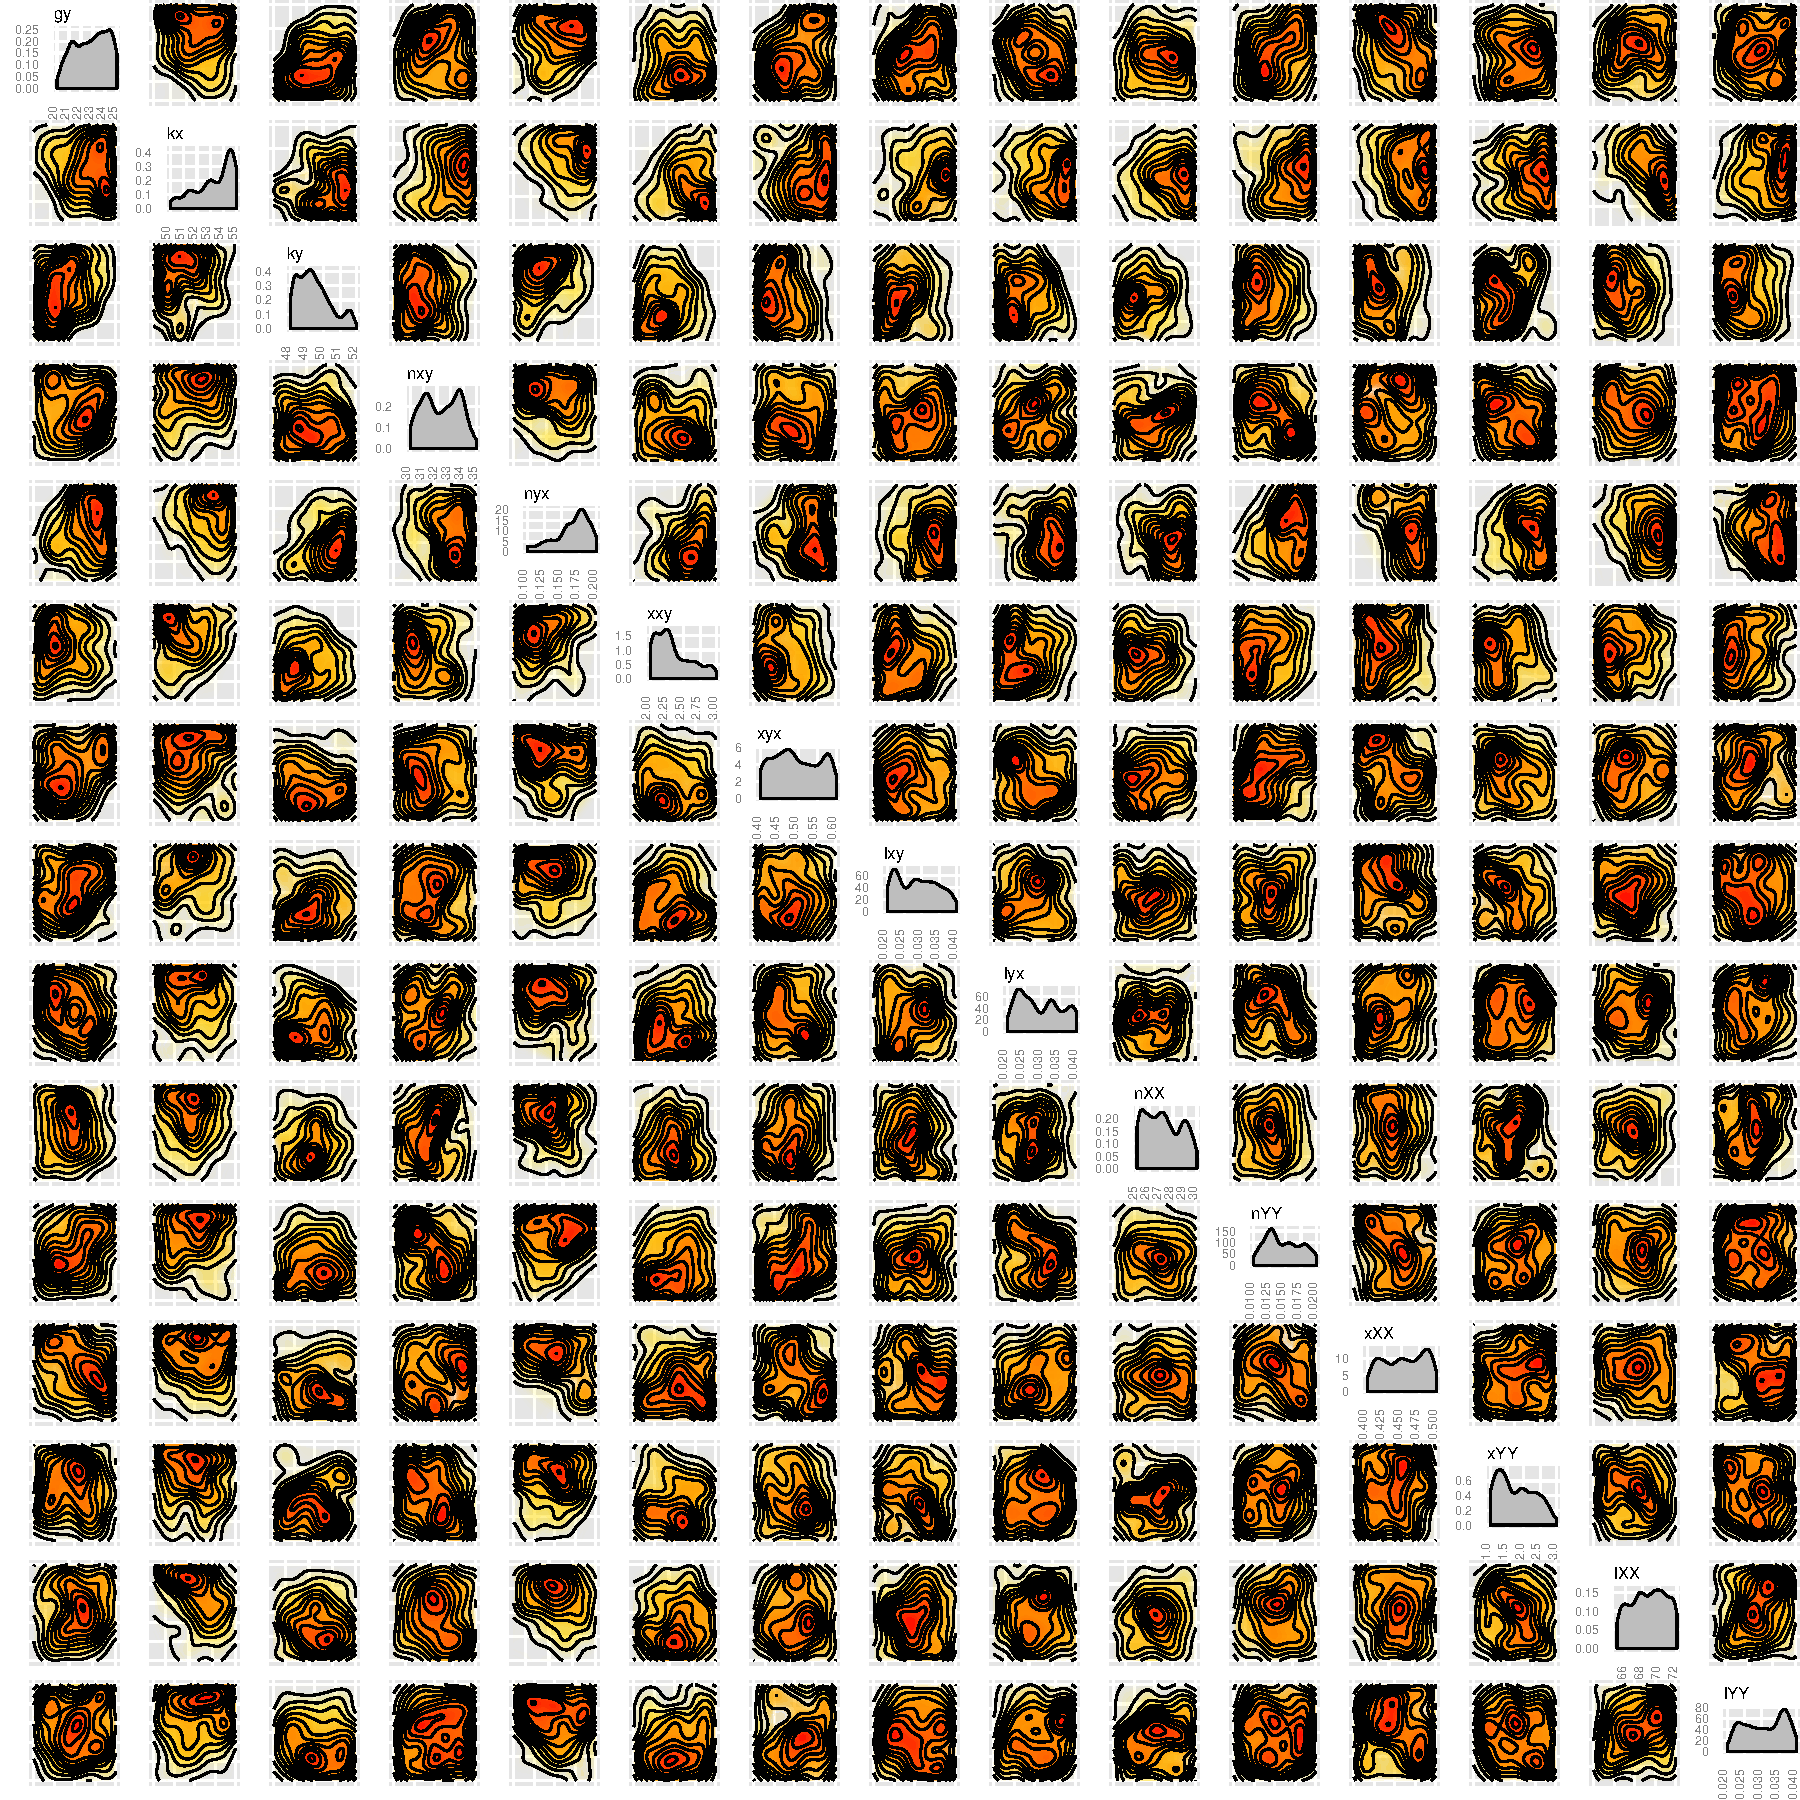
\includegraphics[scale=0.7]{chapterModelling/images/Gardner/posterior.pdf}
\caption[The posterior distribution of the bistable Gardner toggle switch]{The posterior distribution of the bistable Gardner toggle switch. The parameters $a_1$, $a_2$ represent to the effective synthesis rate of repressors 1 and 2 respectively. Parameters $\beta$, $\gamma$ represent the cooperativity on repressors 1 and 2 respectively. The marginal distributions of each parameter are found on the diagonal and pairwise joint distributions along the sides.}
\label{fig:Gard_post}
\end{figure}


\begin{figure}[t]
\centering
\includegraphics[scale=0.3]{chapterModelling/images/Gardner/phase_plots.png}
\caption{A sample of the phase plots produced from the final population of the Gardner switch.}
\label{fig:det_gard_phase}
\end{figure}

\begin{table}[b]
\centering
\caption{Gardner switch priors}
\label{tab:gard}
\begin{tabular}{cccc|cc}
\multicolumn{4}{c|}{Parameters} & \multicolumn{2}{c}{Species} \\ %\hline
$a_1$   & $\beta$   & $a_2$   & $\gamma$  &   $s_1$      &       $s_2$   \\
0-10    & 0-5       & 0-10    &  0-5      &      0-100   &          0-100   
\end{tabular}
\end{table}

These results agree with the results reported by the original paper~\autocite{Gardner:2000vha} . For this switch to be bistable $a_1$ and $a_2$ must be balanced while $\beta$ and $\gamma$ must both be \textgreater 1, as can be seen in the marginal distributions of $\beta$ and $\gamma$ in Figure~\ref{fig:Gard_post}. The conditions set by the original paper for parameters $a_1$ and $a_2$ are met, as the joint distribution shown in Figure~\ref{fig:Gard_post} matches the bifurcation lines calculated in the original paper. 
This successful test demonstrates that StabilityFinder can be used to find the stability a model is capable of as well as the parameter ranges that can produce that. This allows us to confidently apply the methodology to further models.
%-%-%-%-%-%-%%-%-%-%-%-%-%%-%-%-%-%-%-%

\subsubsection{Comparing the deterministic and stochastic cases} 
    
There are two main ways of modelling a system, deterministically and stochastically. Deterministic modelling utilises ordinary differential equations (ODE) and models the concentrations of the species (proteins or other molecules) by time-dependent variables~\autocite{deJong:2002ft}. Rate equations are used to model gene regulation where the rate of production of a species is a function of the concentrations of the other species~\autocite{deJong:2002ft}. When modelling deterministically the model is viewed as a system which, with sufficient knowledge of the system, its behaviour is entirely predictable. Nevertheless we are still a long way away from having complete knowledge of a system of interesting size~\autocite{wilkinson:2006}. Deterministic modelling also assumes a homogenous mixture where species concentrations vary continuously and deterministically, assumptions that often are not met \textit{in vivo}. A cell is spatially and temporally separated, due to small molecule numbers and fluctuations in the timing of processes~\autocite{deJong:2002ft}.  
   
In stochastic modelling, species are measured in discrete amounts rather than concentrations and a joint probability distribution is used to express the probability that at time \textit{t} the cell contains a number of molecules of each species~\autocite{deJong:2002ft}. It takes uncertainty into account and is thus often more appropriate for modelling cellular systems, although more computationally intensive. In stochastic systems the Gillespie algorithm is widely used to simulate the time-evolution of the state of the system~\autocite{Warren:2005kea}.

The toggle switch has been modelled both deterministically and stochastically, with the two methods producing different results. Thus here we use StabilityFinder to compare the stabilities that the model is capable of, under the different simulation types. By using the same framework, and the same prior distributions for the models, one can directly compare the posterior distributions produced by the deterministic and the stochastic case, and uncover the effects that are due to the stochasticity of the system. This is relevant in a a biological model in which small molecule numbers and external noise are not negligible. Using StabilityFinder and using the same priors for the two models (Table~\ref{tab:gard_det_stoch}), we calculated the posterior for each both bistable models. The results are shown in Figure~\ref{fig:Gard_summary}. The prior ranges used are much wider than in the test case in order to allow more flexibility in both models and have a greater range over which to compare the models. 


\begin{table}[h]
\centering
\caption{Gardner switch priors in the deterministic and stochastic cases}
\label{tab:gard_det_stoch}
\begin{tabular}{cccc|cc}
\multicolumn{4}{c|}{Parameters} & \multicolumn{2}{c}{Species} \\ %\hline
$a_1$   & $\beta$   & $a_2$   & $\gamma$  &   $s_1$      &       $s_2$   \\
0-60    & 0-5       & 0-60    &  0-5      &      0-100   &          0-100   
\end{tabular}
\end{table}

\begin{figure}[p]
\centering
\includegraphics[scale=0.45]{chapterModelling/images/Gardner/summary.png}
\caption[The stochastic and deterministic cases of the Gardner toggle switch]{The Gardner toggle switch is modelled stochastically and deterministically. The model is shown graphically and mathematically in (A), The posterior and phase space of the deterministic model is shown in (B) and of the stochastic case in (C).}
\label{fig:Gard_summary}
\end{figure}


%\begin{figure}[p]
%\centering
%\includegraphics[scale=0.5]{chapterModelling/images/Gardner/wide_var/posterior_deter_high_mean.pdf}
%\caption{The posterior distribution of the deterministic model of the Gardner toggle switch.}
%\label{fig:Gard_post_det_high}
%\end{figure}
%
%\begin{figure}[p]
%\centering
%\includegraphics[scale=0.5]{chapterModelling/images/Gardner/wide_var/posterior_stch_high_mean.pdf}
%\caption{The posterior distribution of the stochastic model of the Gardner toggle switch.}
%\label{fig:Gard_post_stch}
%\end{figure}
\clearpage
As can be seen in the above results, stochasticity has a big effect on the posterior. Firstly, a greater parameter range can produce a bistable behaviour when stochastic effects are taken into account. The condition set by T.~S Gardner~\autocite{Gardner:2000vha} for the values of $a_1$ and $a_2$ to be balanced holds in both the deterministic and stochastic cases but in the stochastic case this is met by a wider range of values. The second conditions of $\beta$, $\gamma$ \textgreater 1 also needs to be met in the stochastic case. The posterior of the deterministic model shown in Figure~\ref{fig:Gard_summary}B, parameters $a_1$ and $a_2$ also have an upper limit of values they can take and still create a bistable switch. In order to test this result, we find the roots of the system for large values of  $a_1$ and $a_2$ in order to see if three roots are still found, two stable and one unstable. The results as shown in Figure indicate that the system is still bistable for increasing values of $a_1$ and $a_2$. This suggests that the upper limit found with StabilityFinder is an artefact of the variance limit imposed on the system. In order to find the steady states we impose an accepted distance from a given total variance for each model. When the two clusters of steady state values are too far removed, this increases total variance of the system and would consequently be rejected in StabilityFinder.

\begin{figure}[h]
\centering
\includegraphics[scale=0.6]{chapterModelling/images/Gardner/gardner_solve_roots_a1a2_big.pdf}
\caption[Solving the Gardner toggle switch.]{Solving the Gardner toggle switch. The parameters values used are:  $a_1$, $a_2$ = 100 and $\beta$, $\gamma$ = 2. The system has three roots, of which one was found to be unstable and the other two stable. This result disagrees with that found in StabilityFinder, that $a_1$ and $a_2$ have an upper limit of 30.}
\label{fig:Gard_robst}
\end{figure}

 When stochasticity is taken into account, robustness increases significantly as seen in Figure~\ref{fig:Gard_robst}. This indicates that stochasticity increases the ability of the model to withstand fluctuations in parameter values and still produce the desired bistability. A deterministic model cannot predict this increased robustness.
 
\begin{figure}[h]
\centering
\includegraphics[scale=0.6]{chapterModelling/images/Gardner/wide_var/robustness_comparison.pdf}
\caption{Comparing the robustness of the deterministic and stochastic Gardner switch models}
\label{fig:Gard_robst}
\end{figure}



In order to check if this increase in robustness is caused by the different clustering methods used in the stochastic and deterministic cases, we tested the deterministic case by running the exact same model but using the clustering algorithm used in the stochastic case. Then we compared the robustness using the method outlined above. These results are shown in Figure~\ref{fig:Gard_det_stoch_kmeans}

\begin{figure}[h]
\centering
\includegraphics[scale=0.5]{chapterModelling/images/Gardner/robustness_comparison_gard_stoch_determ_kmeans.pdf}
\caption{The effect of the clustering methods on robustness measurements}
\label{fig:Gard_det_stoch_kmeans}
\end{figure}

This indicates that the clustering methods used have a big effect on the robustness measured. The increase in robustness seen in Figure~\ref{fig:Gard_robst} could be a bias of the clustering algorithms.
\clearpage

%\section{Lu toggle switch models}
 
\subsection{Classical model}
\subsection{Single positive autoregulation}
\subsection{Double positive autoregulation}
\subsection{Extracting the design principles of a tristable switch}

%\section{Mass Action switches}
\subsection{Deterministic case}
\subsubsection{Symmetric switch}
\subsubsection{Asymmetric switch}
\subsubsection{Including transcription and translation}
\subsection{Stochastic case}
\subsubsection{Bistable} 
\subsubsection{Tristable}
\subsubsection{Extracting the design principles of a tristable switch}

%\section{Discussion}

Here we presented a methodology, StabilityChecker, which can identify the region of parameter space that can produce the stability of choice. We demonstrated its use on some known models and extracted stability and robustness information from them. We compared the stability profile of the Gardner toggle switch when modelled deterministically and stochastically in order to uncover the differences that arise from the addition of noise in the modelling. We found that the stochastic model showed increased robustness to noise.

We then applied StabilityChecker to the Lu switches in order to uncover the design principles that make a switch bistable versus tristable. We found that the gene expression parameters were critical for making a tristable switch bistable. This would be in agreement with the dynamics of a tristable switch, in which the third steady state occurs when there is a deadlock situation between the two proteins. When there are small numbers of both proteins involved, one represses the production of the other resulting in both promoters being repressed \autocite{Ma:2012dt}. Given our result we can extrapolate that a higher rate of protein production eliminates the possibility of this deadlock situation happening. Once a promoter is free to produce protein it will produce it in a fast enough rate so that that protein dominates the system and represses the antagonizing promoter before it has the chance to repress it. This dynamic would explain the fact that when all the priors remained the same but gene expression was increased by an order of magnitude, the tristable switch became bistable. 

We also applied StabilityChecker to a synthetic biology design problem. We used two models of the switch, one simple model consisting of two mutually repressive transcription factors and a model with added double positive auto-regulation. Comparing the two models, both capable of bistable behaviour, using StabilityChecker we found that the model with added double positive feedback loops is more robust to parameter fluctuations. This makes it a better candidate for building new synthetic devices based on the toggle switch design. We identified the parameter region within which this models are bistable, information that is important when building such a device in the lab. In the future, by selecting the system components accordingly, the parameter values can be adjusted \textit{in vivo}. For example, the parameter value corresponding to the translation initiation rate can be chosen by selecting the appropriate RBS sequence which given a nucleotide sequence will produce the desired rate \autocite{Holtz:2010bm}, a method developed by Salis \autocite{Salis:2009gk}. Another method to tweak the parameter values \textit{in vivo} is to select the promoter to have the strength corresponding to the levels of gene expression and repression desired. Activity of each promoter can be measured and standardised \autocite{Kelly:2009bj} making this process possible. For a system requiring more than one promoter, these can be efficiently selected from a promoter library using a genetic algorithm created by \textcite{Wu:2011bq}. These standardised interchangeable components with known sequence and activity are what synthetic biology classes as BioBricks \autocite{Kelly:2009bj,Canton:2008fv}. These can be selected and used to construct a desired system and replicate the parameter values found using StabilityChecker.

The methodology we presented here can be applied to a variety of problems as demonstrated. It can be applied to any problem of finding the parameter values that can produce a desired stability between two species. It can be used to design new systems of desired stability and help identify the appropriate parts to use by identifying the rates within which these parts need to operate. It can also be used to examine existing systems and give an insight on the underlying mechanisms that allow for the given stability to occur. 





%%  Characterising the toggle switch -----------------%%
\mainmatter*
\chapter{Bayesian model fitting applied to flow cytometry data}
\label{ch:Flow}
\section{Introduction}
In this chapter, I aim to study the genetic toggle switch experimentally.  This chapter is organised as follows: In the first section I provide an overview of the circuit used and then outline the methods used for the experiments carried out. In the subsequent section I investigate the effect that the switch has on the growth rate of the bacteria. Then I examine the concentrations of the inducers and the time needed to flip the switch. 


\section{Flow cytometry and model fitting}

Flow cytometry detects the fluorescent intensity levels in individual cells. It can also provide physical information about the size and granularity of a cell via the forward and side scattering respectively. An overview of flow cytometry is shown in Figure~\ref{fig:flow_overv}. A laser excites the fluorochrome present in the bacterial cells. The fluorochromes emit a signal that is detected by channels in the optics. The signals are then all collected and analysed. A sample typically consists single cell measurements of $10^4$-$10^5$ cells. %Typically the cell populations are separated from the noise in the experiment via expert manual gating. Advances in flow cytometry technology has increased both the number of the dimensions of the datasets and the number of samples obtained, thus promoting the development for automated methods~\autocite{Johnsson:2016fd, Chen:2015bp, ONeill:2013cs}.



\begin{figure*}[tb]
	\begin{center}
		\includegraphics[scale=0.9]{../../chapters/chapterABCFlow/images/flow-overview.png}
	\caption[LoF caption]{\label{fig:flow_overv}: Flow cytometry. A laser excites the fluorescent proteins present in each cell. The cytometer has up to 4 lasers, violet (V), red (R), yellow (Y) and blue (B). The detectors in the optics, FL1-4 pick up the signals. The cytometer also picks up size and granularity information via the forward scatter (FSC) and side scatter (SSC) detectors. }
	\end{center}
\end{figure*}


Flow cytometry is used in synthetic biology, among others, for BioBrick characterisation~\autocite{Kelly:2009bj}, enzyme screening~\autocite{Choi:2014gb} and industrial  bioprocesses~\autocite{Diaz:2010kw}. Flow cytometry is a powerful tool for synthetic biology as it can measure multiple parameters in single cells, and process up to 35,000 cells sec\textsuperscript{-1}~\autocite{Anonymous:2015tj}. 

A drawback of flow cytometry is that the fluorescence intensity per cell is measured rather than number of proteins. Measuring absolute numbers of protein would be ideal for model fitting, but this type of biological data cannot be directly measured~\autocite{Kelwick:2014iy}. Standardization of experimental methods in flow cytometry has aided the effort to convert relative measurements, like fluorescence intensity, to absolute measurements, like GFP cell\textsuperscript{-1} s\textsuperscript{-1}~\autocite{Kelly:2009bj, Kelwick:2014iy}. 

In this chapter, I developed ABC-Flow, a method to fit computational models to experimental flow cytometry data. ABC-Flow approaches the problem of absolute protein numbers by converting the model output of GFP cell\textsuperscript{-1} s\textsuperscript{-1} to relative fluorescence intensity. ABC-Flow is a python package that uses Bayesian statistics to fit the parameters of a given model to flow cytometry time course data. The algorithm and its usage is described in Section~\ref{sec:abcflow-meth}.

%Progress has been made in the development of computational tools for the automated analysis of flow cytometry data from the field of computational immunology~\autocite{Saeys:2016im}. These tools are used for automated gating~\autocite{Lo:2008it, Aghaeepour:2011fv, Johnsson:2016fd} as well as modelling of cellular processes over time~\autocite{Bendall:2014hs, Bagwell:2015gp}. These methods are used to track different subpopulations over time, in order to follow the underlying developmental trajectory~\autocite{Saeys:2016im} and thus cannot be applied to experiments involving uniform cell populations. 


% is necessary as flow cytometry measures the intensity of the fluorescent proteins of interest in each cell.

 %On the other hand, when simulating a model, the output is measured in number of fluorescent proteins. It is thus essential to convert the simulated signal to the same format as the data, thus convert the number of fluorescent proteins to intensity measures. 
\section{ABC-Flow algorithm development}
\label{sec:abcflow-meth}

The algorithm of ABC-Flow is based on the same ABC algorithm as ABC-SysBio and Stability Finder described in Sections (XXX), adapted to be used for flow cytometry data. The algorithm of ABC-Flow is outlined in Algorithm~\ref{alg:abc-flow}. The modified modules of the ABC algorithm are outlined in the sections that follow.

\begin{figure*}[htbp]
	\begin{center}
		\includegraphics[scale=0.7]{../../chapters/chapterABCFlow/images/abc-flow-overv.png}
		\caption[LoF caption]{\label{fig:abcflow-overv}: Overview of ABC-Flow. (A) ABC-Flow is used to fit models to experimental flow cytometry data. (B) The algorithm can be applied to 1D and 2D flow data. (C) ABC-Flow uses approximate bayesian computation.}
	\end{center}
\end{figure*}

The user provides an SBML model file and an input file to specify the information needed to run ABC-Flow, like the \epsilon schedule and the priors to the parameters. The user must also provide a data file containing the flow cytometry data to which the model will be fitted. The data files used here were generated from .fcs files, which is the standard output of flow cytometers using the R bioconductor packages flowCore~\autocite{flowCore:man}. ABC-Flow simulations are implemented on \acrshort{gpu}s.



\begin{algorithm}[htbp]

\caption{ABC-Flow}
\label{alg:abc-flow}
 \begin{algorithmic}[1]
 	\Statex
% \State Read input file
%	\If{ABC-Rejection}
% 		\State Sample from priors
% 		\State Simulate model
% 		\State Convert signal to intensity
% 		\State Measure distance to data
%		\State Reject particles if d $\textgreater$ $\epsilon$.
% 		\If{number of accepted particles == number of particles}
% 			\State Exit
% 		\Else
% 			\State Return to step 3.
% 		\EndIf
% 	\EndIf
 	
 	%\If{ABC-SMC}
	\State Initialise $\epsilon$ 
	\Let{population p}{1}
	\If{p $= 1$}
		\State Sample particles ($\theta$) from priors
		\Else
			\State Sample particles from previous population
			\State Perturb each particle by $\pm$ half the range of the previous population (j) to obtain new perturbed population (i).
	\EndIf
	\State Simulate model
	\State Convert signal to intensity: 
	\For{each particle}
		\For{each beta}
			\For{each timepoint}
				\For{each fluorescent protein}
					\State Intensity = N\bigg(signal\times$\mu$,  $\sqrt{(signal\times\sigma^2)}$\bigg)
	\EndFor				
	\EndFor	
	\EndFor	
	\EndFor	
	\State Measure distance to data
	\State Reject particles if d $\textgreater$ $\epsilon$.
    \State Calculate weight for each accepted $\theta$
	\State $w_{t}^{(i)} = \begin{cases} 1, & \mbox{if } p = 0 \\\frac{\pi(\theta_{t}^{(i)})}{\sum_{j=1}^N w_{t-1}^{(j)} K_{t}(\theta_{t-1}^{(j)}, \theta_{t}^{(i)})}, & \mbox{if } p \geq  0. \end{cases}$
	\State Normalise weights
	\State Repeat steps 3 - 15 until $\epsilon \leq \epsilon_T$	%EndIf
  \end{algorithmic}
\end{algorithm}

\clearpage
\subsubsection{Distance Calculations}


\begin{algorithm}[htbp]
\label{alg:dist}
\caption{Distance calculation}
 \begin{algorithmic}[1]
    \Statex
	\Let {Grid}{min(data):max(data):ngrid} 
	\State kD = kernel density estimation(data)
	\State kS = kernel density estimation(simulations)
	\State fD = kD(xx)
	\State fS = kS(xx)    
	\State $d = \sum((fD-fS)^2)$
  \end{algorithmic}
\end{algorithm}

Next, by varying the amount of $\mu$ and $\sigma$ by which the two normals differ, we can find out the dynamical range of the epsilons. Whether two distributions are identical or vary by a large amount, we can get an estimate of how much the epsilon will vary from one to the other, both in 1D and 2D. 

\begin{figure}[htbp]
\centering
\includegraphics[scale=0.5]{../../chapters/chapterABCFlow/images/mus_sigmas_diff.png}
\caption[LoF caption]{ (A)The range by which epsilon varies as the difference between the $\mu$ of the distributions increases. (B) The difference between the epsilon distribution medians in the 1D and 2D case is not constant with increasing $\mu$ difference between the data sets. (C)The variance of the epsilon distributions remains relatively constant with increasing $\mu$. (D)The median of the epsilon distributions varies by a small amount with increasing difference in the $\sigma$ of the distributions, but the variance (E) remains relatively constant.}
\label{fig:epsilon_mu_s_diff}
\end{figure}


\begin{figure}[htbp]
\centering
\includegraphics[scale=0.6]{../../chapters/chapterABCFlow/images/multimodal_musd.png}
\caption[LoF caption]{Comparing the 1D and 2D distances between bimodal distributions. (A) and (B) show samples of the bimodal distributions compared in 1D and 2D respectively with a $\mu$ difference of 4 between simulations and data. (C,D) The range by which epsilon median and variance varies as the difference between the $\mu$ of the distributions increases.}
\label{fig:multimodal_musd}
\end{figure}
\clearpage

\begin{figure}[htbp]
\centering
\includegraphics[scale=0.6]{../../chapters/chapterABCFlow/images/multimodal_v_normal.png}
\caption[LoF caption]{Comparing a multimodal to a normal distribution, in 1D and 2D. (A, B) We vary the $mu$ of the normal distribution from equal to the $\mu$ of the first peak of the bimodal distribution to beyond the range of the bimodal distribution. (C) We find that epsilon median and variance are at the lowest when the $\mu$ of the normal distribution is equal to the $\mu$ of one of the peaks of the bimodal distribution. }
\label{fig:multimodal_v_normal}
\end{figure}





The distance in the 1D case was calculated using the Kolmogorov-Smirnov test~\autocite{Kolmogorov:1933}. The Kolmogorov-Smirnov test is a non-parametric statistic test that determines whether the two distribution functions differ. The KS distance between two distributions is equal to the largest distance between the empirical distribution functions of the two samples, as illustrated in Figure~\ref{fig:ks-dist} and Equation~\ref{eq:ks1d}.

\begin{align}
\label{eq:ks1d}
D_{n,n'}=\sup _{x}|F_{1,n}(x)-F_{2,n'}(x)|
\end{align}



\begin{figure*}[htbp]
\begin{center}
	\includegraphics[scale=0.5]{../../chapters/chapterABCFlow/images/ks-1d-overv.png}
			\caption[LoF caption]{\label{fig:ks-dist}:The Kolmogorov-Smirnov distance function used to calculate the distance between distributions in the 1D case.}
	\end{center}
\end{figure*}



%A grid is first defined, from the minimum to the maximum value in the dataset. A gaussian kernel is fit to the experimental and the simulated data, at each timepoint for the given grid. The distance between the two kernels is then defined by:

%\begin{align*}%
%	d = \sum_{i=xmin}^{xmax} (fD_i - fS_i)^2
%\end{align*}


For the 2D case the distance was calculated in a similar way, by using an adaptation of the Kolmogorov-Smirnov distance in higher dimensions~\autocite{Peacock:1983fa}.

%\begin{figure*}[htbp]
%	\begin{center}
%		\includegraphics[scale=0.8]{../../chapters/chapterABCFlow/images/KS-dist.png}
%		\caption[LoF caption]{\label{fig:ks-dist}:The Kolmogorov-Smirnov distance function used to calculate the distance between distributions in the 1D (A) and 2D (B) cases.}
%	\end{center}
%\end{figure*}
%\clearpage
\clearpage
\subsubsection{Intensity calculation}

The units of the result of the stochastic simulations is in the form of number of fluorescent proteins. On the other hand, flow cytometry data units are in the form of fluorescence intensity. For ABC-Flow, the simulation results are converted to intensity in order to be able to compare the data to the simulations. In order to do this two additional parameters are defined, intensity \textmu{} and intensity \textsigma{}, for each fluorescent protein used. To convert the number of fluorescent proteins to intensity, random samples are drawn from a normal distribution:

\begin{align}
	X\sim N\Big(nFP\times\mu, \sqrt{(nFP\times\sigma^2)}\Big), \label{eq:intens}
\end{align}
where nFP is the number of fluorescent proteins. 


These parameters are fitted to the data along with the model parameters.  

\begin{figure*}[htbp]
	\begin{center}
		\includegraphics[scale=0.6]{../../chapters/chapterABCFlow/images/intensity_calc.png}
		\caption[LoF caption]{\label{fig:intensity_calc}:Converting the number of fluorescent proteins to the intensity (iFP) is done by drawing from a normal distribution, as shown in Equation~\ref{eq:intens}.}
	\end{center}
\end{figure*}

\subsection{ABC-Flow model fitting }

In order to characterise the~\textcite{Litcofsky:2012gr} toggle switch, I use the data collected in Section~\ref{sec:ts_time} to fit the~\textcite{Gardner:2000vha} toggle switch model, shown in Section (XXX). In order to do that, I use ABC-Flow as described in the Methods in Section~\ref{sec:abcflow-meth}.

%Prior to using ABC-Flow to fit the experimental data to a toggle switch model, ABC-Flow must be validated. In the following sections I first use randomly generated distributions to set the algorithm metrics and distances. Then I use a simulated data set to which I fit a toggle switch model and finally I use ABC-Flow to fit experimental data.  

In the following sections I first use normal distributions to study the distance functions used in ABC-Flow. Then I use a simulated data set to which I fit a toggle switch model and finally I use ABC-Flow to fit experimental data.  

\subsubsection{Distance study}
%Here I simulate two normal distributions, with identical mu and sigma, and calculate the distance between the two using the distance measure used in ABC-Flow. Doing this 1000 times, we then plot the distribution of epsilon. By doing that we can calculate the variance of the epsilon distribution, and find out the error that can be expected when measuring the distance in ABC-Flow. By doing that in 1D and in 2D we can compare the epsilon variances. 

Here, I simulate two normal distributions, with $\mu=0$ and $\sigma=1$ and measure the distance between them using the Kolmogorov-Smirnov test, as used in ABC-Flow. Doing this multiple times, the expected variation in distance values for identical distributions can be calculated. This is the error that can be expected when measuring distance in ABC-Flow. As can be seen in Figure~\ref{fig:epsilon_boxplt}, there range of distance values obtained in the 1D case is small, as the distance between two data sets drawn from the same distribution ranges from 0.1 to 0.2. For the 2D case, the distance values obtained vary more than in the 1D case. 


\begin{figure}[htbp]
\centering
\includegraphics[scale=0.7]{../../chapters/chapterABCFlow/images/epsilon_same_box.png}
\caption[LoF caption]{\label{fig:epsilon_boxplt} The distance between two data sets drawn form the same distribution are compared using the Kolmogorov-Smirnov two sample test. (A) in 1D and (B) in 2D. (C) The distance is calculated for 1000 data sets. A greater variation of values is found for the 2D distance calculation.  }
\label{fig:normal_example}
\end{figure}
\clearpage


To further study the distance calculation used in ABC-Flow, the data sets are drawn from increasingly different distributions, and the distance between them calculated. As shown in Figure~\ref{fig:epsilon_mud}, the 1D distance is 0 when the difference between the \textmu{} from which the two datasets are drawn is 0.5 or less, and 1 when the difference in the \textmu{} between the two data sets is 7 or larger. In the 2D case the standard deviation of the calculated distance is larger than the 1D case. The distance calculation reaches a plateau at epsilon = 2.3 when the \textmu{} difference is 3 or larger. As shown in Figure~\ref{fig:epsilon_mud}D, as the number of samples drawn from each distribution increases, the standard deviation of the distance calculations decreases in the 1D case. This trend is less obvious in the 2D case.
\begin{figure}[htbp]
\centering
\includegraphics[scale=0.7]{../../chapters/chapterABCFlow/images/mu_diff.png}
\caption[LoF caption]{\label{fig:epsilon_mud} The distance calculation for data sets drawn from increasingly different distributions. Two examples are shown of distributions compared in (A) 1D and (B) 2D. (C) As the difference between the means of the two distributions increases, the distance calculation, epsilon, increases. In the 2D case (shown in green) epsilon plateaus at 2.3 and in the 1D case (shown in blue) epsilon plateaus at 1.}
\label{fig:normal_example}
\end{figure}



%The next parameter to be optimised is the bin size used in the distance calculation. In both 1D and 2D, the space is divided into bins, and the distance between corresponding bins in the data and the simulated data is calculated. The overall distance between to distributions is the sum of the distances between corresponding bins. %If the bin size is too large, small differences between 


%We find that the 2D distance is more sensitive to the bin size than the 1D distance. From Figure~\ref{fig:epsilon_ngrid} we conclude that for a sample size of 100 data points, the optimal bin size for 1D and 2D distance calculation is 10. The above optimizations have been made by using standard normal distributions, of $\mu=0$ and $\sigma=1$. Here we investigate whether the distance calculation depends on the $\mu$ and $sigma$ of the distributions. 

%Next, by varying the amount of $\mu$ and $\sigma$ by which the two normals differ, we can find out the dynamical range of the epsilons. Whether two distributions are identical or vary by a large amount, we can get an estimate of how much the epsilon will vary from one to the other, both in 1D and 2D. 


%From Figure~\ref{fig:epsilon_mu_s_diff} we find that as the difference in $\mu$ increases the epsilon medians reach a plateau. We find that beyond a difference of 4 in $\mu$, the distance calculation cannot further separate the distances. This can be caused by the fact that when first dividing the space into bins, the range of the data is used to define the grid. If all the simulated data is located outside that grid, the algorithm can no longer distinguish between them, and will only allocate them as outside the range. The variance of the epsilon distributions does not vary significantly with increasing difference in $\mu$. As the difference in $\sigma$ increases between the distributions, we find that the median in the 2D distance calculation increases but not in the 1D. Note, that the range of the difference in the epsilon medians is small and thus we conclude that differences in the $\mu$ of a distribution are much better detected than the differences in the $\sigma$. The variance of the epsilon distribution when $\sigma$ is varied does not change significantly with increasing $\sigma$ difference.


%We study the epsilon distribution variance in the uniform distribution, [0, 1].  
%When comparing a normally distributed data set to a uniformly distributed data set, we don't see a great difference between the 1D and 2D epsilons.


%Another type of distribution that is commonly found in Flow cytometry experiments, is a bimodal distribution. Here we test whether the 1D and 2D distances are equivalent when measuring distances in this type of distributions.


%Finally, we study how the distances perform when comparing a bimodal with a normal distribution. We test the distances by using a bimodal distribution and a series of normal distributions with increasing $\mu$, in 1D and 2D. We find that epsilon is the lowest when the $\mu$ of the normal distribution corresponds to the $\mu$ of one of the two peaks in the bimodal distribution and the highest when there is no overlap between the distributions. 



\clearpage
\subsubsection{ABC-Flow validation using simulated data}

In this section I apply ABC-Flow to simulated data, where the parameter values used to produce the data are known. This analysis will serve as a verification test for ABC-Flow. The model used to produce the simulated data is an extension of the~\textcite{Gardner:2000vha} switch. The model consists of two mutually repressing transcription factors. The model used here has additional parameters, representing the repression from the external repressors, \acrshort{iptg} and \acrshort{atc}. 

In order to produce the simulated data set, the extended~\textcite{Gardner:2000vha} switch was simulated stochastically using the Gillespie algorithm~\autocite{Gillespie:1977ww}. The model used is defined by the following hazards:

\begin{align}
h_1 &= u \label{eq:eg1}\\
h_2 &= \frac{p_1 \times p_3	}{1+p_3+v^{p_2}} \label{eq:eg2}\\
h_3 &= (1 + a)\times v \label{eq:eg3}\\
h_4 &= \frac{p_4\times p_6}{1+p_6+u^{p_5}} \label{eq:eg4}
\end{align}


Using the time course data generated for one of the fluorescent proteins in the system, $u$, I use ABC-Flow to fit the model shown above, using priors centered around the parameter values used to produce the data. The resulting fit is shown in Figure~\ref{fig:1d-sim-res}A. In order to determine whether this is a good fit to the data, QQ plots are produced for each timepoint (Figure~\ref{fig:1d-sim-res}B). A QQ-plot is a plot where the quantiles of two distributions are plotted against eachother. If the distributions are similar, the points will lie on the 45\textdegree{} line x = y line~\autocite{Wilk:1968ts}. 


\begin{figure}[htbp]
\centering
	\includegraphics[scale=0.8]{../../chapters/chapterABCFlow/images/1D_sim_res.png}
	\caption[LoF caption]{\label{fig:1d-sim-res} (A) 1D ABC-Flow fit (shown in blue) to data (shown in red) produced by simulating the same model. (B) QQ-plot of each time point fit. The quantile of the two distributions are plotted against eachother. If the ditributions are similar, the points would lie on the 45\textdegree{} line x = y, shown in red. }
\end{figure}
\clearpage

By examining the data and the fitted models shown in Figure~\ref{fig:1d-sim-res}, we see that at \textepsilon = 0.1, there is a good fit of the model to the data using ABC-Flow. The model parameters, as well as the intensity parameters, have been fitted to simulated flow cytometry data. The timecourse of the model after fitting with ABC-Flow is similar to the data time course. 

I further test ABC-Flow by using 2D data to fit two species of the model simultaneously. The same data was used as was used in the 1D case, but this time both species $u$ and $v$ were taken into account. This represents both sides of the switch model used. Using the same priors as in the 1D case, we can compare the two fits and investigate whether using the 1D or 2D data results in a better fit. The 1D data represents one of the marginal distributions of the data sets, as illustrated in Figure~\ref{fig:1d2dsketch}. I use the marginal distribution of $u$ and the bivariate distribution of $u$ and $v$ in order to determine which one produces a better fit to the data. The resulting timecourse of the data as well as the 1D and 2D fit are shown in Figure~\ref{fig:1d2dcomp}.


\begin{figure}[htbp]
\centering
\includegraphics[scale=0.3]{../../chapters/chapterABCFlow/images/normal_sigma_example.png}
\caption[LoF caption]{\label{fig:1d2dsketch} The marginal (1D) versus the bivariate (2D) distribution of the data.}
\end{figure}




\begin{figure}[htbp]
\centering
\includegraphics[scale=0.8]{../../chapters/chapterABCFlow/images/1d2dfit.png}
\caption[LoF caption]{\label{fig:1d2dcomp} Comparing the fits obtained by using the 1D or 2D data. }
\end{figure}
\clearpage


The posterior distributions obtained from each fit are shown in Figure~\ref{fig:1d2d-sim-post}. We find similar posterior ranges for both the 1D and 2D fits.

\begin{figure}[htbp]
\centering
	\includegraphics[scale=0.4]{../../chapters/chapterABCFlow/images/sim_1d_2d_post.pdf}
	\caption[LoF caption]{\label{fig:1d2d-sim-post} 1D (red) 2D (blue) fit. }
\end{figure}

%\begin{figure}[htbp]
%\centering%
%	\includegraphics[scale=0.6]{../../chapters/chapterABCFlow/images/1d_sim_post.png}%
%	\caption[LoF caption]{\label{fig:1d-sim-post}}
%\end{figure}



%\begin{figure}[htbp]
%\centering
%	\includegraphics[scale=0.6]{../../chapters/chapterABCFlow/images/2D_sim_res.png}
%	\caption[LoF caption]{\label{fig:2d-sim-res}}
%\end{figure}


\section{Toggle switch data collection}
\subsection{Circuit overview}

The toggle switch plasmid I used here was provided by ~\textcite{Litcofsky:2012gr}. All the switch components were contained in one plasmid, pKDL071. An overview of the plasmid is shown in Figure~\ref{fig:pKDL071map}A and the sequence given in Appendix (XXX). The circuit consists of two promoters, Ptrc2 and PLtetO-1~\autocite{Lutz:1997ti}. Ptrc2 is a constitutive promoter, repressible by LacI. PLtetO-1 is also a constitutive promoter, repressible by TetR, as shown in Figure~\ref{fig:pKDL071map}B. mCherry~\autocite{Shaner:2004vy} and \acrshort{gfp}~\autocite{SHIMOMURA:1962va} are fluorescent proteins, that were added under the control of the same promoters as the repressors, and thus reflect the levels of TetR and LacI in the system. The plasmid contains kanamycin antibiotic resistance and is high copy (ColE1 origin of replication).

This system is capable of two states, GFP high and mCherry high. When \acrshort{iptg} is added to the system, it represses the repression of TetR and mCherry and thus the cells end up in the mCherry high state. When \acrshort{atc} is added to the system, it represses the repression of LacI and GFP and thus the cells end up in the GFP high state. If no inducer is added to the system it will randomly go to the GFP high or mCherry high states.

\begin{figure*}[tb]
	\begin{center}
		\includegraphics[scale=0.55]{../../chapters/chapterABCFlow/images/pKDL071_overview.png}
	\caption[LoF caption]{\label{fig:pKDL071map}: The genetic toggle switch circuit used in this chapter. (A) The plasmid map of pKDL071, the plasmid containing the genetic toggle switch used in~\textcite{Litcofsky:2012gr} (B) The interactions between each element of the circuit.}
	\end{center}
\end{figure*}
\clearpage


\subsection{Methods}

The toggle switch plasmid was provided by the James J Collins lab in the form of a stab culture in \textit{E. coli} K-12 MG1655.

\subsubsection{\textit{Escherichia coli} culturing conditions}
\label{sec:overnigh_cult}

\acrfull{lb} was made by diluting \acrshort{lb} in deionized water to a concentration of \SI{25}{\gram\per\liter} and subsequently autoclaved. \acrshort{lb} agar plates were made by adding bacteriological agar to the above solution to a concentration of \SI{45}{\milli\gram\per\milli\liter} before autoclaving. The solution was then cooled down to \SI{55}{\celsius} using a water bath. If antibiotic was required it was added to the correct concentration to the cooled solution. The solution was then aliquoted to plates and left to solidify in room temperature. The plates were stored in the fridge for up to 1 month. 


Overnight cultures were made by picking a single colony from a static culture in an agar plate. Each colony was placed in \SI{15}{\milli\liter} Falcon tubes (Fisher Scientific, MA, U.S.A) with \SI{5}{\milli\liter} \acrshort{lb} with kanamycin antibiotic at a concentration of \SI{50}{\micro\gram\per\milli\liter}. The tubes were then screwed loosely and taped securely in order to allow for aeration. The falcon tubes were put in an incubator at \SI{37}{\celsius} with orbital shaking at \SI{200} rpm for 12-16 hours. 

\subsubsection{Glycerol stock preparation}
\label{sec:glycerol_stock}
To preserve the transformed cultures long-term glycerol stocks were made. \SI{5}{\milli\liter} \acrshort{lb} and Kanamycin overnight cultures were made as described in Section~\ref{sec:overnigh_cult}. The cultures were kept on ice and \SI{70}\% glycerol was added to the cultures in a ratio of glycerol to culture of 1:7. These were aliquoted into cryovials and transferred to a \SI{-80}{\celsius} freezer for long-term storage.


\subsubsection{Revival}
For subsequent revival of the frozen cultures, a \SI{1.5}{\milli\liter} eppendorf tube was removed from the \SI{-80}{\celsius} freezer and put on ice. Small amount was streaked onto an agar plate containing \acrshort{lb} and kanamycin. The plates were stored in an incubator at \SI{37}{\celsius} overnight. Then the plates were sealed using parafilm and stored at \SI{4}{\celsius} for up to two weeks. 

\subsubsection{Inducers}

Anhydrotetracycline (ATc) solution was made by diluting \acrshort{atc} from Cayman Chemical Company in \SI{100}\% ethanol to a concentration of \SI{1}{\milli\gram\per\milli\liter}. \acrfull{iptg} solution was made by dissolving \acrshort{iptg} in deionized water to a concentration of \SI{1}{\molar}. The solution was sterilised by passing the solution through a \SI{0.22}{\micro\meter} syringe filter. Both inducers were stored in \SI{1}{\milli\liter} aliquots at \SI{-20}{\celsius}. 


\subsubsection{Growth rate measurement}
\label{sec:growth_meth}
Plate reader analysis was carried out in order to measure the growth of \textit{E.coli} over time. Overnight cultures were made using the method shown in Section~\ref{sec:overnigh_cult}. Overnight cultures were then diluted by a 1:1000 ratio into a \SI{5}{\milli\liter} \acrshort{lb} + kanamycin solution. The diluted cultures were grown at \SI{37}{\celsius} with shaking at 200rpm for 1 hour. These cultures were then further diluted by a 1:100 ratio. \SI{200}{\ul} aliquots of the dilutions were then transferred to a clear bottom, black-walled 96-well plate. Wells with only LB and kanamycin were also added in order to be used as blanks. The plate was then sealed using a gas permeable membrane and placed it in BMG FLUOstat OPTIMA plate reader to measure absorbance. The plate reader was set to a constant \SI{37}{\celsius}, with 30 seconds orbital shaking at \SI{150}rpm and \SI{4}{\milli\metre} shaking width every ten minutes. Absorbance was measured at \SI{540}{\nano\meter}. Data was exported as a CSV file and analysed using Python. 

\subsubsection{Flow cytometry}
Flow cytometry experiments were carried out in order to get fluorescent levels in single cells. Flow cytometry allows us to gather this information for thousands of single cells. Flow cytometry data was exported as FCS files and analysed using the R bioconductor packages flowCore~\autocite{flowCore:man}, flowViz~\autocite{flowViz:man} and Ggplot2~\autocite{ggplot2:bk}. 

\subsubsection{Concentration assays}
\label{sec:flo_conc}
Concentration assays were carried out in order to determine the concentration of each inducer (\acrshort{atc} and \acrshort{iptg}) at which the switch flips.  Separate overnight cultures were prepared as per Section~\ref{sec:overnigh_cult} with added \acrshort{iptg} at a concentration of \SI{1}{\milli\molar} or added \acrshort{atc} at a concentration of \SI{100}{\nano\gram\per\milli\liter}~\autocite{Litcofsky:2012gr}. The cultures were then diluted by 1:1000 into fresh \acrshort{lb} medium with varying concentrations of the opposite inducer than what the cells were grown in overnight. The concentrations used are shown in Table~\ref{tab:flow_conc}. For each concentration. three replicates cultures were made.


\begin{table}[htbp]
\centering
\caption{Concentrations used for flow cytometry assay}
\label{tab:flow_conc}
\begin{tabular}{@{}cc@{}}
\toprule
\acrshort{atc} (ng/ml)  & \acrshort{iptg} (M) \\ \midrule
0.05 & 1e-7 \\
0.06 & 6e-7 \\
0.07 & 1e-6 \\
0.08 & 6e-6 \\
0.09 & 1e-5 \\
0.1  & 1e-3 \\
1.0  & 0.1  \\ \bottomrule
\end{tabular}
\end{table}

The cultures were placed in an incubator at \SI{37}{\celsius}, 200rpm for 5 hours. The cultures were then placed in a centrifuge and spun at 13,000rpm for 5 minutes. The supernatant was discarded and replaced it with \SI{1}{\milli\liter} PBS solution. The BD LSRFortessa\textsuperscript{TM} cell analyzer (Becton, Dickinson and Company) was used at the St. Mary's Flow Cytometry Core Facility at Imperial College London  for flow cytometry analysis. \acrshort{gfp} was excited using the \SI{488}{\nano\meter} laser and detected using the 533/30 filter. mCherry was excited using the \SI{561}{\nano\meter} laser and detected using the 620/10 filter. Data was obtained at n=10000 events per experiment. 

\subsubsection{Time course assays}
\label{sec:flo_time}
Time course assays were carried out to measure the time it takes for the switch to flip to each state. Separate overnight cultures of pKDL071 were prepared as per Section~\ref{sec:overnigh_cult} with added \acrshort{iptg} at a concentration of \SI{1}{\milli\molar} or added \acrshort{atc} at a concentration of \SI{100}{\nano\gram\per\milli\liter}~\autocite{Litcofsky:2012gr}. Overnight cultures of pSEVA281G and pSEVA281C were also made. The cultures were then diluted by a ratio of 1:1000 into fresh LB medium. Separate cultures for each time point were made, in triplicate. For cultures grown overnight in \acrshort{iptg}, \acrshort{atc} was added at a concentration of \SI{100}{\nano\gram\per\milli\liter} and for cultures grown overnight in \acrshort{atc}, \acrshort{iptg} was added at a concentration of \SI{1}{\milli\molar}. All cultures were placed at \SI{37}{\celsius}, 200rpm incubator. At 30 minutes, 1 hour and then every hour up to 6 hours flow cytometry was carried out for the corresponding cultures. Triplicates for each induction were removed from the incubator and placed in a centrifuge at 13, 000rpm for 10 minutes. The supernatant was discarded and replaced with \SI{1}{\milli\liter} PBS solution. These cultures were then analysed in an Attune\textsuperscript{TM} NxT Flow Cytometer (Thermo Fisher Scientific) at University College London. \acrshort{gfp} was excited using the \SI{488}{\nano\meter} laser and detected using the 533/30 filter. mCherry was excited using the \SI{561}{\nano\meter} laser and detected using the 620/10 filter. Data was obtained at n=10000 events per experiment. pSEVA281G and pSEVA281C cultures were used to set the laser voltages and pKDL071 cultures to detect the bacteria population.  


\subsection{Results}
\subsubsection{Growth rate investigation}

I carried out a growth rate analysis to determine whether the \acrshort{atc} or \acrshort{iptg} added to pKDL071 or pSEVA281G \textit{E. coli} cultures affected the growth of the bacteria. Cultures were grown without any inducer overnight as described in Section~\ref{sec:growth_meth}. I ran assays for the cultures with and without added inducers. As can be seen in Figure~\ref{fig:growth_curve}, there is no difference between the conditions. The addition of either \acrshort{atc} or \acrshort{iptg} does not affect the growth rate of \textit{E. coli} K-12 MG1655. Additionally, \acrshort{atc} does not affect the growth rate of \textit{E. coli} Dh5\textalpha. Since the addition of \acrshort{atc} flips the switch to the GFP high state, and \acrshort{iptg} to the mCherry high state, we can also conclude that the growth rate of the chassis is not affected by which side of the switch is in the high state. The growth rate of \textit{E. coli} Dh5\textalpha was consistently lower than that of \textit{E. coli} K-12 MG1655.

\begin{figure*}[htbp]
	\begin{center}
		\includegraphics[scale=0.7]{../../chapters/chapterABCFlow/images/growth_curves.pdf}
		\caption[LoF caption]{\label{fig:growth_curve}: Growth rate analysis of \textit{E. coli} K-12 MG1655 pKDL071 and \textit{E. coli} Dh5\textalpha pSEVA281G cultures with and without inducers. The inducers do not affect the growth of the bacteria. }
	\end{center}
\end{figure*}

\clearpage

\subsubsection{Toggle switch concentration assays}

Here I aim to identify the inducer concentration at which the pKDL071 toggle switch changes state. In order to do that I carry out a concentration assay using flow cytometry, as described in Section~\ref{sec:flo_conc}. As can be seen in Figure~\ref{fig:switch_concent2d1d}A, during \acrshort{atc} induction the switch flips to a GFP high state when \acrshort{atc} concentration is at \SI{0.09}{\nano\gram\per\milli\liter} or higher. We observe a bimodal distribution at concentrations \SI{0.07}{\nano\gram\per\milli\liter} and \SI{0.08}{\nano\gram\per\milli\liter}, which indicates that the switching has begun at these concentrations. Thats why part of the population has switched to the GFP high state but complete switching is not observed until the concentration of \acrshort{atc} is at \SI{0.09}{\nano\gram\per\milli\liter}. In the case of \acrshort{iptg} induction (Figure~\ref{fig:switch_concent2d1d}B) we find that the switch flips to the mCherry high state when the concentration of \acrshort{iptg} is higher or equal to 0.001M. A decrease in GFP fluorescence is also observed. We do not observe a bimodal distribution in this case. 

\begin{figure*}[htbp]
	\begin{center}
\includegraphics[scale=0.7]{../../chapters/chapterABCFlow/images/pKDL071_concentrations_2d1d.png}
\caption[LoF caption]{\label{fig:switch_concent2d1d}: (A) \acrshort{atc} induction at various concentrations (B) \acrshort{iptg} induction at various concentrations. }
\end{center}
\end{figure*}
\clearpage

By taking into account the two induction curves of the switch turning to each high state, we can see the dynamic ranges of pKDL071 in \textit{E.coli}. We can see in Figure~\ref{fig:switch_concentrations_model} there is an approximately 100-fold change in fluorescent units during \acrshort{iptg} and \acrshort{atc} induction. 

 A Hill function was used to model the characterisation curves shown in Figure~\ref{fig:switch_concentrations_model}. The model used is the following:
 \begin{align}
 	F = Pmin + (Pmax - Pmin)\frac{\Big(\frac{[I]}{Kd}\Big)^n}{1+\Big(\frac{[I]}{Kd}\Big)^n},
 \end{align}
 
where F is the median fluorescent unit and [I] is the concentration of inducer. Pmin and Pmax are the minimum and maximum fluorescence respectively, and Kd and n are the dissociation constant, and Hill coefficient. I fit Hill function models using maximum likelihood estimation to the response curves. The values for parameters Pmin, Pmax, Kd, and n are 8, 1600, 0.1, 1.8 respectively for the \acrshort{atc} induction and 8, 700, 0.08, 2.5 for \acrshort{iptg} induction. 

\begin{figure*}[tb]
	\begin{center}
\includegraphics[width=\textwidth]{../../chapters/chapterABCFlow/images/pKDL071_concentrations_model_fit.png}
\caption[LoF caption]{\label{fig:switch_concentrations_model}: (A, B) \acrshort{atc} induction of pKDL071. (C, D) \acrshort{iptg} induction of pKDL071.}
\end{center}
\end{figure*}


For the case of the \acrshort{atc} induction we observe a sharp switch between the GFP low to the GFP high state, as can be seen in the characterisation curve in Figure~\ref{fig:switch_concentrations_model}B. This is a clear indication of the bistability of this switch.

\clearpage





\subsubsection{Toggle switch time course assay}
\label{sec:ts_time}
I further analysed the pKDL071 toggle switch by investigating the time it takes for it to switch from one high state to the other. To do that I used the method outlined in Section~\ref{sec:flo_time}. I obtained separate time courses for the \acrshort{iptg} and \acrshort{atc} inductions. 

As can be seen in Figure~\ref{fig:switch_timecourse_atc} pKDL071 \acrshort{atc}  induction begins switching 1 hour after induction. Complete induction is seen at 6 hours. During the \acrshort{iptg} induction (Figure~\ref{fig:switch_timecourse_iptg}) we see a bimodal distribution at 4 hours, and induction is complete at 6 hours. We observe that during \acrshort{atc} induction there is an increase in \acrshort{gfp} fluorescence and a decrease in mCherry fluorescence, in the case of \acrshort{iptg} induction the increase in mCherry fluorescence is not as prominent. A decrease in GFP fluorescence is observed during \acrshort{iptg} induction. 

\begin{figure*}[tb]
	\begin{center}
\includegraphics[scale=0.7]{../../chapters/chapterABCFlow/images/pKDL071_atc_time.png}
\caption[LoF caption]{\label{fig:switch_timecourse_atc}: \acrshort{atc} induction of pKDL071 over time}
\end{center}
\end{figure*}


\begin{figure*}[tb]
	\begin{center}
\includegraphics[scale=0.7]{../../chapters/chapterABCFlow/images/pKDL071_iptg_time.png}
\caption[LoF caption]{\label{fig:switch_timecourse_iptg}: \acrshort{iptg} induction of pKDL071 over time}
\end{center}
\end{figure*}
\clearpage


%\begin{figure*}[tb]
%	\begin{center}
%\includegraphics[scale=0.5]{../../chapters/chapterABCFlow/images/atc_timecourse.png}
%\caption[LoF caption]{\label{fig:atc_timecourse}: \acrshort{atc} induction of pKDL071 over time}
%\end{center}
%\end{figure*}
%
%\begin{figure*}[tb]
%	\begin{center}
%\includegraphics[scale=0.5]{../../chapters/chapterABCFlow/images/iptg_timcourse.png}
%\caption[LoF caption]{\label{fig:iptg_timecourse}: \acrshort{iptg} induction of pKDL071 over time}
%\end{center}
%\end{figure*}
%\clearpage

\subsubsection{Plasmid construction}

I constructed two plasmids in order to use them for the flow cytometry experiments. The first plasmid, pSEVA281G contains the promoter PLtetO-1 and \acrshort{gfp} and the other, pSEVA281C, contains the promoter Ptrc2 and mCherry from PKDL071, shown in Figure~\ref{fig:psevas}. These two plasmids were used to determine the appropriate voltages for the lasers that excite \acrshort{gfp} and mCherry.

pSEVA281G was constructed by digesting pKDL071 and pSEVA281 using the protocol outlined in Section~\ref{sec:digest}. pSEVA281 is a plasmid backbone containing kanamycin resistance, a high copy origin of replication and a multiple cloning site. The digested fragments were isolated using gel purification (Section~\ref{sec:gel_electr}) and then ligated the isolated fragments (Section~\ref{sec:ligation}). \textit{Escherichia coli} Dh5\textalpha{} was then transformed with each plasmid (Section~\ref{sec:transfection}). pSEVA281C was constructed via \acrshort{pcr} cloning. \acrshort{pcr} was carried out using the pKDL071 plasmid as a template \acrshort{dna} using the protocol outlined in Section~\ref{sec:pcr}. Primers were chosen so that Ptrc2 and mCherry were copied and a Hind\RNum{3} restriction enzyme recognition sequence added to the fragment. The primers are listed in Appendix (XXX). The amplified \acrshort{dna} was purified using the Qiagen PCR cleanup kit (Qiagen, Crawley, U.K) and then carried out the rest of the cloning procedure as per plasmid pSEVA281G.

Following construction, each plasmid was isolated using the QIAprep Spin Miniprep Kit (Qiagen, Crawley, U.K). Plasmid concentration was determined using the Thermo Scientific NanoDrop 1000 Spectrophotometer (Fisher Scientific, MA, U.S.A).

\begin{figure*}[t]
	\begin{center}
		\includegraphics[width=\textwidth]{../../chapters/chapterABCFlow/images/plasmids_constructed.png}
		\caption[LoF caption]{\label{fig:psevas}: The plasmids used to calibrate GFP and mCherry fluorescence. (A) pSEVA281G plasmid map (B) pSEVA281C plasmid map.  }
	\end{center}
\end{figure*}

\subsubsection{Polymerase Chain Reaction}
\label{sec:pcr}
In order to amplify DNA and add the restriction enzyme sites required, a \acrfull{pcr} reaction was carried out with mutagenic primers. A list of primers can be found in Appendix (XXX). Q5\textsuperscript{\textregistered} DNA Polymerase (NEB, MA, U.S.A) was used with its associated buffer, \acrshort{dntp} and Q5\textsuperscript{\textregistered} enhancer, as specified in Table~\ref{tab:pcr_rec}. \acrshort{pcr} reactions were run in a T100\textsuperscript{TM} thermal cycler (Bio-Rad Laboratories, Inc., UK) as per the Q5\textsuperscript{\textregistered} recommendations, and as outlined in Tables~\ref{tab:pcr_rec} and ~\ref{tab:pcr_sched}.

\begin{table}[H]
\centering
\caption{\acrshort{pcr} recipe}
\label{tab:pcr_rec}
\begin{tabular}{@{}ccc@{}}
\toprule
Reagent           & Final concentration & \SI{50}{\micro\liter} reaction \\ \midrule
Q5\textsuperscript{\textregistered} buffer 5X      & 1X                  & \SI{10}{\micro\liter}          \\
\acrshort{dntp}             & \SI{200}{\milli\molar} each          & \SI{1}{\micro\liter}           \\
Forward primer    & \SI{0.5}{\micro\molar}               & \SI{2.5}{\micro\liter}         \\
Reverse primer    & \SI{0.5}{\micro\molar}               & \SI{2.5}{\micro\liter}         \\
Template DNA      & \SI{2}{\micro\gram}/\SI{50}{\micro\liter}                 & -             \\
Q5\textsuperscript{\textregistered} \acrshort{dna} polymerase & \SI{0.02}{\unit\per\micro\liter}            & \SI{0.5}{\micro\liter}         \\
Q5\textsuperscript{\textregistered} enhancer       & 1X                  & \SI{10}{\milli\liter}          \\
\ce{H2O}               & -                   & to \SI{50}{\micro\liter}       \\ \bottomrule
\end{tabular}
\end{table}


\begin{table}[H]
\centering
\caption{Thermocycling conditions}
\label{tab:pcr_sched}
\begin{tabular}{@{}cccc@{}}
\toprule
Step            & Cycles              & Temperature           & Time                 \\ \midrule
Initiation      & 1                   & \SI{98}{\celsius} & \SI{30}{\second} \\
Denaturation    & \multirow{3}{*}{30} & \SI{98}{\celsius} & \SI{10}{\second} \\
Annealing        &                     & \SI{72}{\celsius} & \SI{20}{\second} \\
Extension       &                     & \SI{72}{\celsius} & \SI{2}{\minute}  \\
Final extension & 1                   & \SI{72}{\celsius} & \SI{2}{\minute}  \\
Hold            & 1                   & \SI{4}{\celsius}  & \infty            \\ \bottomrule  
\end{tabular}
\end{table}

\subsubsection{Digestion}
\label{sec:digest}

All enzymes, buffers and \acrfull{bsa} were supplied by NEB. Digestion controls were carried out by adding \ce{H2O} instead of \acrshort{dna} in the digestion reaction. Additionally, during agarose gel electrophoresis uncut plasmid was run alongside the digested plasmid in order to detect the difference. 

\SI{2}{\micro\gram} digests were set up by mixing the plasmid with \SI{0.5}{\micro\liter} of each restriction enzyme, \SI{3}{\micro\liter} 10x buffer and \SI{3}{\micro\liter} 10x \acrshort{bsa}. \ce{H2O} was added to make the reaction to \SI{20}{\micro\liter}. The recipe used is shown in Table~\ref{tab:digestion}. The reactions were placed in an incubator at \SI{37}{\celsius} for 4 hours. Finally, the solutions were analysed using agarose gel electrophoresis (Section~\ref{sec:gel_electr}).


\begin{table}[htbp]
\centering
\caption{Digestion recipe}
\label{tab:digestion}
\begin{tabular}{@{}cccc@{}}
\toprule
Reagent   & Volume  &  &  \\ \midrule
Pst\RNum{1}&                \SI{0.5}{\micro\liter}     &  &  \\
Hind\RNum{3} &                \SI{0.5}{\micro\liter}     &  &  \\
NEB Buffer 2.1        & \SI{2}{\micro\liter}       &  &  \\
BSA            & \SI{0.2}{\micro\liter}     &  &  \\
\acrshort{dna}              & \SI{1}{\micro\gram}       &  &  \\
\ce{H2O}           & to \SI{20}{\micro\liter} &  &  \\ \bottomrule
\end{tabular}
\end{table}


\subsubsection{Agarose gel electrophoresis}
\label{sec:gel_electr}
To make a 0.8\% agarose gel, \SI{0.4}{\gram} agarose were diluted in \SI{50}{\milli\liter} 1X TAE buffer. It was further dissolved by microwaving for 1-3 minutes. The solution was left to cool for 5 minutes and then \SI{1.5}{\micro\liter} gel red were added. Gel trays were prepared by putting the well comb in place and taping the ends shut. The solution wast then poured into the prepared gel trays and left to solidify for 20-30 minutes at room temperature.

Agarose gel electrophoresis was carried out by placing the poured gels into the gel tanks. The tank was then flooded with 1X TAE buffer. The \acrshort{dna} was prepared to be analysed by adding \SI{4}{\micro\liter} loading dye to \SI{20}{\micro\liter} sample. A negative control was used with \ce{H2O} instead of sample. The \acrshort{dna} ladder of choice was prepared by adding \SI{1}{\micro\liter} \ce{H2O} and \SI{1}{\micro\liter} dye to \SI{2}{\micro\liter} ladder. Each sample was added to a well by pipetting. The agarose gel was ran at \SI{90}{\volt} until the dye was 80\% of the way down the gel, approximately 1 hour.

To purify the fragments from the agarose gel, the gel was placed in a UV box. Using a sterile razor blade, the desired fragment was cut out and placed in a clean eppendorf tube. The \acrshort{dna} was isolated from the gel using the QIAquick Gel Extraction Kit.

\subsubsection{Ligation}
\label{sec:ligation}
A ratio of 3:1 of insert to recipient plasmid was used, \SI{1}{\micro\liter} T4\textsuperscript{\textregistered}  DNA ligase (NEB, MA, U.S.A) and \SI{2}{\micro\liter} ligase buffer. \ce{H2O} was added to make the reaction up to \SI{20}{\micro\liter}. The controls used for each ligation reaction, are shown in Table~\ref{tab:lig-contr}. Control 1 is used to detect competent cell viability, control 2 background due to uncut vector, control 3 contamination and control 4 vector re-circularization.  

The ligation reactions were placed at \SI{4}{\celsius} for 12 hours. The reactions were then placed at \SI{65}{\celsius} for 10 minutes to heat inactivate the T4 DNA ligase enzyme. A transformation was then carried out as per Section~\ref{sec:transfection}.

\begin{table}[htbp]
\centering
\caption{Ligation controls}
\label{tab:lig-contr}
\begin{tabular}{@{}ccccc@{}}
\toprule
       & Control 1 & Control 2 & Control 3 & Control 4 \\ \midrule
Vector &  Uncut    & \cmark    & \cmark    & \xmark    \\
Insert &  \xmark    & \xmark    & \xmark    & \cmark    \\
Buffer &  \cmark    & \cmark    & \cmark    & \cmark    \\
\ce{H2O}    & \cmark    & \cmark    & \cmark    & \cmark    \\
Ligase &  \xmark    & \xmark    & \cmark    & \cmark    \\ \bottomrule
\end{tabular}
\end{table}


\subsubsection{Transformation}
\label{sec:transfection}
Thermocompetent \textit{E.coli} Dh5\textalpha was transformed with the constructed plasmids. Each ligation reaction was added to \SI{50}{\micro\liter} of thawed competent cells. The cells were subsequently kept on ice for 30 minutes, then placed at a \SI{42}{\celsius} water bath for \SI{45}{\second}. The cells were then placed back on ice for 15 minutes. Then \SI{500}{\micro\liter} of Super Optimal broth with Catabolite repression (SOC) were added to each ligation and placed in a \SI{37}{\celsius} shaking incubator for 3 hours. \SI{500}{\micro\liter} and \SI{50}{\micro\liter} were subsequently pipetted of each ligation onto petri dishes with LB agar and the appropriate antibiotic. The plates were incubated at \SI{37}{\celsius} for 12-16 hours. Two controls were used for the transfection protocol, a positive control with no antibiotic in the LB agar and non-transfected cells and a negative control of non-transformed cells and LB agar with antibiotic. These ensure that the cells are viable and not contaminated respectively. 

Finally, the number of colonies were counted on each plate. Individual colonies were then selected from each transfection and grew each separately in \SI{5}{\milli\liter} LB medium for 12-16 hours at \SI{37}{\celsius}, 200 rpm. Glycerol stocks were then prepared from each culture, as per Section~\ref{sec:glycerol_stock}.



\subsubsection{Colony \acrshort{pcr}}

In order to determine if the fragment was successfully inserted into the vector \acrshort{dna} plasmid, diagnostic colony \acrshort{pcr} was then carried out. Primers were designed that amplified the multiple cloning site of the vector \acrshort{dna} plasmid. These can be found in Appendix (XXX). A \acrshort{pcr} master mix was made for the number of colonies to be amplified, 32, with an added 10\% to account for pipetting error. GoTaq\textsuperscript{\textregistered} Flexi \acrshort{dna} polymerase (Promega Corp., WI, U.S.A.) was used with its associated buffer, \acrshort{dntp} and \ce{MgCl2}and \ce{H2O}. The recipe for the master mix is shown in Table~\ref{tab:pcr_mastex_mix}.

\begin{table}[htbp]
\centering
\caption{Colony \acrshort{pcr} master mix recipe}
\label{tab:pcr_mastex_mix}
\begin{tabular}{@{}ccc@{}}
\toprule
Reagent           & Final concentration & Master mix \\ \midrule
GoTaq\textsuperscript{\textregistered} green Flexi buffer      & 1X                  & \SI{141}{\micro\liter}          \\
\acrshort{dntp}             & \SI{200}{\milli\molar} each          & \SI{14.1}{\micro\liter}           \\
Forward primer    & \SI{0.5}{\micro\molar}               & \SI{1.4}{\micro\liter}         \\
Reverse primer    & \SI{0.5}{\micro\molar}               & \SI{1.4}{\micro\liter}         \\
GoTaq\textsuperscript{\textregistered} Flexi polymerase & \SI{0.02}{\unit\per\micro\liter}            & \SI{3.5}{\micro\liter}         \\
\ce{MgCl2}       & 1X                  & \SI{42.2}{\micro\liter}          \\
\ce{H2O}               &     -               & \SI{465}{\micro\liter}       \\ \bottomrule
\end{tabular}
\end{table}

\SI{19}{\micro\liter} were then added from the master mix to each \acrshort{pcr} tube. Each of the colonies was then lifted from the transformation from the agar plate using a \SI{20}{\micro\liter} pipette tip and added it to a \acrshort{pcr} mix by mixing. The pipette tip was subsequently used to make a scratch into a clean agar plate, and labelled it. A \acrshort{pcr} was then carried out according to GoTaq\textsuperscript{\textregistered} Flexi polymerase recommendations, and as shown in Table~\ref{tab:pcr_sched_col}.

\begin{table}[H]
\centering
\caption{Thermocycling conditions for colony \acrshort{pcr}}
\label{tab:pcr_sched_col}
\begin{tabular}{@{}cccc@{}}
\toprule
Step            & Cycles              & Temperature           & Time                 \\ \midrule
Cell lysis      & 1                   & \SI{95}{\celsius} & \SI{10} minutes \\

Denaturation    & \multirow{3}{*}{35} & \SI{95}{\celsius} & \SI{30}{\second} \\
Annealing        &                     & \SI{50}{\celsius} & \SI{1} minute \\
Extension       &                     & \SI{72}{\celsius} & \SI{1}{\minute}  \\

Final extension & 1                   & \SI{72}{\celsius} & \SI{5}{\minute}  \\
Hold            & 1                   & \SI{4}{\celsius}  & \infty            \\ \bottomrule  
\end{tabular}
\end{table}

Finally a diagnostic agarose gel electrophoresis was carried out as outlined in Section~\ref{sec:gel_electr}.

\subsubsection{Sequencing}
In order to confirm plasmid identity, all plasmids were sequenced using Source Bioscience, Cambridge UK. \SI{10}{\micro\liter}  of each plasmid DNA were submitted at a minimum of \SI{100}{\nano\gram\per\micro\liter} as per the requirements. Primer sequences were also submitted and manufactured by Source Bioscience. Primers can be found in Appendix (XXX). 




\clearpage
\section{ABC-Flow used on experimental data}
 
Next I applied ABC-Flow to the experimental flow cytometry data collected in Section~\ref{sec:ts_time}. The data set is comprised of time course data of the~\textcite{Litcofsky:2012gr} toggle switch. The two states of the switch are represented by the levels of GFP and mCherry intensity in each bacterial cell. Using \acrshort{atc} inducer, each cell transitions from a mCherry high state to a GFP high state. I used the extension to the~\textcite{Gardner:2000vha} switch described in Equations~\ref{eq:eg1}-\ref{eq:eg4}.

 
\begin{figure}[htbp]
\centering
	\includegraphics[scale=0.6]{../../chapters/chapterABCFlow/images/1D_real_res.png}
	\caption[LoF caption]{\label{fig:1d-real-res}}
\end{figure}




%\subsubsection{\acrshort{atc} induction}
 
 
%\begin{figure}[htbp]
%\centering
%\includegraphics[scale=0.5]{../../chapters/chapterABCFlow/images/real_dat/real_dat_2D.png}
%\caption[LoF caption]{Real data 2D fit}
%\label{fig:real_dat_2d}
%\end{figure}
%\clearpage

%\subsubsection{\acrshort{iptg} induction}
\section{Discussion}

Here I characterised the genetic toggle switch experimentally. First I study the effect of the two inducers \acrshort{atc} and \acrshort{iptg} on the growth rate of the selected chassis \textit{E. coli} K-12 MG1655. I find that there is no detrimental effect to the bacterium by the inducers. I also find that which state the switch is on has no effect on the growth rate of the bacteria. In order for this toggle switch to be used in a synthetic biology application, it is important that both sides of the switch have an equivalent burden onto the chassis. If one of the steady states creates a larger burden and slows down the growth of the bacteria, this can create an imbalance in the population. If the toggle switch-bearing bacterial population exists in an environment with competing bacteria, for example the gut microbiome, and one of the two states creates a larger burden, this would cause the switch-bearing population to become less competitive compared to the non switch-bearing population. It is therefore crucial that the state of the switch does not affect the competitiveness of the chassis.  


I further characterised the switch by determining the minimum inducer concentration necessary to change the state of the switch. I find that for \acrshort{atc} induction, a minimum of \SI{0.09}{\nano\gram\per\milli\liter} is required to cause the switch to go to a GFP high state. For \acrshort{iptg} induction I find that a minimum of \SI{0.001}{M} is required to flip the switch to an mCherry high state. This information is critical for using this switch in other applications. Both sides of the switch are very sensitive to inducer concentrations, as the concentrations required to observe a change in fluorescence are very small. 

Furthermore I find that this toggle switch, pKDL071, is faster to respond to a change in \acrshort{atc} concentration that to a change in \acrshort{iptg} concentration. For \acrshort{iptg} induction we observe a change in fluorescence after 3-4 hours of induction. For \acrshort{atc} induction we can see a difference within an hour of induction. This result is in agreement with~\textcite{Litcofsky:2012gr}. This difference in response times must be taken into account when using the pKDL071 switch for other applications. This difference could be due to maturation times of the fluorescent proteins. \textcite{Macdonald:2012el} found that mCherry half-maturation time is 150 mins, whereas the GFP variant used here, GFPmut3b has been especially mutated for fast action~\autocite{Cormack:1996gv}. ~\textcite{Cormack:1996gv} found that whereas wild type GFP is detectable 1-2 hours after induction, GFPmut3b is detectable 8 minutes after induction. This difference could account for the different response times observed here, but further investigation is required. 


\section{Summary}


In this chapter I summarised the experiments carried out for the analysis of the genetic toggle switch. I used the pKDL071 plasmid and characterised its switching behaviour over various inducer concentrations and over time. I found the concentration of each inducer necessary to flip the switch as well as the time it takes for the change to be observed. Furthermore, I investigated the effect of the inducers on the growth rate of the chassis and found that they have no effect. In the next chapter I use the data collected in the chapter to fit to the more realistic toggle switch models used in Chapter (XXX). 





 
 
%\section{Introduction}
In this chapter, I aim to study the genetic toggle switch experimentally.  This chapter is organised as follows: In the first section I provide an overview of the circuit used and then outline the methods used for the experiments carried out. In the subsequent section I investigate the effect that the switch has on the growth rate of the bacteria. Then I examine the concentrations of the inducers and the time needed to flip the switch. 


\section{Flow cytometry and model fitting}

Flow cytometry detects the fluorescent intensity levels in individual cells. It can also provide physical information about the size and granularity of a cell via the forward and side scattering respectively. An overview of flow cytometry is shown in Figure~\ref{fig:flow_overv}. A laser excites the fluorochrome present in the bacterial cells. The fluorochromes emit a signal that is detected by channels in the optics. The signals are then all collected and analysed. A sample typically consists single cell measurements of $10^4$-$10^5$ cells. %Typically the cell populations are separated from the noise in the experiment via expert manual gating. Advances in flow cytometry technology has increased both the number of the dimensions of the datasets and the number of samples obtained, thus promoting the development for automated methods~\autocite{Johnsson:2016fd, Chen:2015bp, ONeill:2013cs}.



\begin{figure*}[tb]
	\begin{center}
		\includegraphics[scale=0.9]{chapterABCFlow/images/flow-overview.png}
	\caption[LoF caption]{\label{fig:flow_overv}: Flow cytometry. A laser excites the fluorescent proteins present in each cell. The cytometer has up to 4 lasers, violet (V), red (R), yellow (Y) and blue (B). The detectors in the optics, FL1-4 pick up the signals. The cytometer also picks up size and granularity information via the forward scatter (FSC) and side scatter (SSC) detectors. }
	\end{center}
\end{figure*}


Flow cytometry is used in synthetic biology, among others, for BioBrick characterisation~\autocite{Kelly:2009bj}, enzyme screening~\autocite{Choi:2014gb} and industrial  bioprocesses~\autocite{Diaz:2010kw}. Flow cytometry is a powerful tool for synthetic biology as it can measure multiple parameters in single cells, and process up to 35,000 cells sec\textsuperscript{-1}~\autocite{Anonymous:2015tj}. 

A drawback of flow cytometry is that the fluorescence intensity per cell is measured rather than number of proteins. Measuring absolute numbers of protein would be ideal for model fitting, but this type of biological data cannot be directly measured~\autocite{Kelwick:2014iy}. Standardization of experimental methods in flow cytometry has aided the effort to convert relative measurements, like fluorescence intensity, to absolute measurements, like GFP cell\textsuperscript{-1} s\textsuperscript{-1}~\autocite{Kelly:2009bj, Kelwick:2014iy}. 

In this chapter, I developed ABC-Flow, a method to fit computational models to experimental flow cytometry data. ABC-Flow approaches the problem of absolute protein numbers by converting the model output of GFP cell\textsuperscript{-1} s\textsuperscript{-1} to relative fluorescence intensity. ABC-Flow is a python package that uses Bayesian statistics to fit the parameters of a given model to flow cytometry time course data. The algorithm and its usage is described in Section~\ref{sec:abcflow-meth}.

%Progress has been made in the development of computational tools for the automated analysis of flow cytometry data from the field of computational immunology~\autocite{Saeys:2016im}. These tools are used for automated gating~\autocite{Lo:2008it, Aghaeepour:2011fv, Johnsson:2016fd} as well as modelling of cellular processes over time~\autocite{Bendall:2014hs, Bagwell:2015gp}. These methods are used to track different subpopulations over time, in order to follow the underlying developmental trajectory~\autocite{Saeys:2016im} and thus cannot be applied to experiments involving uniform cell populations. 


% is necessary as flow cytometry measures the intensity of the fluorescent proteins of interest in each cell.

 %On the other hand, when simulating a model, the output is measured in number of fluorescent proteins. It is thus essential to convert the simulated signal to the same format as the data, thus convert the number of fluorescent proteins to intensity measures. 

\section{Circuit overview}

The toggle switch plasmid I used here was provided by ~\textcite{Litcofsky:2012gr}. All the switch components were contained in one plasmid, pKDL071. An overview of the plasmid is shown in Figure~\ref{fig:pKDL071map}A and the sequence given in Appendix (XXX). The circuit consists of two promoters, Ptrc2 and PLtetO-1~\autocite{Lutz:1997ti}. Ptrc2 is a constitutive promoter, repressible by LacI. PLtetO-1 is also a constitutive promoter, repressible by TetR, as shown in Figure~\ref{fig:pKDL071map}B. mCherry~\autocite{Shaner:2004vy} and \acrshort{gfp}~\autocite{SHIMOMURA:1962va} are fluorescent proteins, that were added under the control of the same promoters as the repressors, and thus reflect the levels of TetR and LacI in the system. The plasmid contains kanamycin antibiotic resistance and is high copy (ColE1 origin of replication).

This system is capable of two states, GFP high and mCherry high. When \acrshort{iptg} is added to the system, it represses the repression of TetR and mCherry and thus the cells end up in the mCherry high state. When \acrshort{atc} is added to the system, it represses the repression of LacI and GFP and thus the cells end up in the GFP high state. If no inducer is added to the system it will randomly go to the GFP high or mCherry high states.

\begin{figure*}[tb]
	\begin{center}
		\includegraphics[scale=0.55]{chapterCharacterisation/images/pKDL071_overview.png}
	\caption[LoF caption]{\label{fig:pKDL071map}: The genetic toggle switch circuit used in this chapter. (A) The plasmid map of pKDL071, the plasmid containing the genetic toggle switch used in~\textcite{Litcofsky:2012gr} (B) The interactions between each element of the circuit.}
	\end{center}
\end{figure*}
\clearpage


\section{Methods}

The toggle switch plasmid was provided by the James J Collins lab in the form of a stab culture in \textit{E. coli} K-12 MG1655.

\subsection{\textit{Escherichia coli} culturing conditions}
\label{sec:overnigh_cult}

\acrfull{lb} was made by diluting \acrshort{lb} in deionized water to a concentration of \SI{25}{\gram\per\liter} and subsequently autoclaved. \acrshort{lb} agar plates were made by adding bacteriological agar to the above solution to a concentration of \SI{45}{\milli\gram\per\milli\liter} before autoclaving. The solution was then cooled down to \SI{55}{\celsius} using a water bath. If antibiotic was required it was added to the correct concentration to the cooled solution. The solution was then aliquoted to plates and left to solidify in room temperature. The plates were stored in the fridge for up to 1 month. 

Overnight cultures were made by picking a single colony from a static culture in an agar plate. Each colony was placed in \SI{15}{\milli\liter} Falcon tubes (Fisher Scientific, MA, U.S.A) with \SI{5}{\milli\liter} \acrshort{lb} with kanamycin antibiotic at a concentration of \SI{50}{\micro\gram\per\milli\liter}. The tubes were then screwed loosely and taped securely in order to allow for aeration. The falcon tubes were put in an incubator at \SI{37}{\celsius} with orbital shaking at \SI{200} rpm for 12-16 hours. 

\subsection{Inducers}

Anhydrotetracycline (ATc) solution was made by diluting \acrshort{atc} from Cayman Chemical Company in \SI{100}\% ethanol to a concentration of \SI{1}{\milli\gram\per\milli\liter}. \acrfull{iptg} solution was made by dissolving \acrshort{iptg} in deionized water to a concentration of \SI{1}{\molar}. The solution was sterilised by passing the solution through a \SI{0.22}{\micro\meter} syringe filter. Both inducers were stored in \SI{1}{\milli\liter} aliquots at \SI{-20}{\celsius}. 

\subsection{Glycerol stock preparation}
\label{sec:glycerol_stock}
To preserve the transformed cultures long-term glycerol stocks were made. \SI{5}{\milli\liter} \acrshort{lb} and Kanamycin overnight cultures were made as described in Section~\ref{sec:overnigh_cult}. The cultures were kept on ice and \SI{70}\% glycerol was added to the cultures in a ratio of glycerol to culture of 1:7. These were aliquoted into cryovials and transferred to a \SI{-80}{\celsius} freezer for long-term storage.


\subsection{Revival}
For subsequent revival of the frozen cultures, a \SI{1.5}{\milli\liter} eppendorf tube was removed from the \SI{-80}{\celsius} freezer and put on ice. Small amount was streaked onto an agar plate containing \acrshort{lb} and kanamycin. The plates were stored in an incubator at \SI{37}{\celsius} overnight. Then the plates were sealed using parafilm and stored at \SI{4}{\celsius} for up to two weeks. 


\subsection{Plasmid construction}

I constructed two plasmids in order to use them for the flow cytometry experiments. The first plasmid, pSEVA281G contains the promoter PLtetO-1 and \acrshort{gfp} and the other, pSEVA281C, contains the promoter Ptrc2 and mCherry from PKDL071, shown in Figure~\ref{fig:psevas}. These two plasmids were used to determine the appropriate voltages for the lasers that excite \acrshort{gfp} and mCherry.

pSEVA281G was constructed by digesting pKDL071 and pSEVA281 using the protocol outlined in Section~\ref{sec:digest}. pSEVA281 is a plasmid backbone containing kanamycin resistance, a high copy origin of replication and a multiple cloning site. The digested fragments were isolated using gel purification (Section~\ref{sec:gel_electr}) and then ligated the isolated fragments (Section~\ref{sec:ligation}). \textit{Escherichia coli} Dh5\textalpha{} was then transformed with each plasmid (Section~\ref{sec:transfection}). pSEVA281C was constructed via \acrshort{pcr} cloning. \acrshort{pcr} was carried out using the pKDL071 plasmid as a template \acrshort{dna} using the protocol outlined in Section~\ref{sec:pcr}. Primers were chosen so that Ptrc2 and mCherry were copied and a Hind\RNum{3} restriction enzyme recognition sequence added to the fragment. The primers are listed in Appendix (XXX). The amplified \acrshort{dna} was purified using the Qiagen PCR cleanup kit (Qiagen, Crawley, U.K) and then carried out the rest of the cloning procedure as per plasmid pSEVA281G.

Following construction, each plasmid was isolated using the QIAprep Spin Miniprep Kit (Qiagen, Crawley, U.K). Plasmid concentration was determined using the Thermo Scientific NanoDrop 1000 Spectrophotometer (Fisher Scientific, MA, U.S.A).

\begin{figure*}[t]
	\begin{center}
		\includegraphics[width=\textwidth]{chapterCharacterisation/images/plasmids_constructed.png}
		\caption[LoF caption]{\label{fig:psevas}: The plasmids used to calibrate GFP and mCherry fluorescence. (A) pSEVA281G plasmid map (B) pSEVA281C plasmid map.  }
	\end{center}
\end{figure*}

\subsubsection{Polymerase Chain Reaction}
\label{sec:pcr}
In order to amplify DNA and add the restriction enzyme sites required, a \acrfull{pcr} reaction was carried out with mutagenic primers. A list of primers can be found in Appendix (XXX). Q5\textsuperscript{\textregistered} DNA Polymerase (NEB, MA, U.S.A) was used with its associated buffer, \acrshort{dntp} and Q5\textsuperscript{\textregistered} enhancer, as specified in Table~\ref{tab:pcr_rec}. \acrshort{pcr} reactions were run in a T100\textsuperscript{TM} thermal cycler (Bio-Rad Laboratories, Inc., UK) as per the Q5\textsuperscript{\textregistered} recommendations, and as outlined in Tables~\ref{tab:pcr_rec} and ~\ref{tab:pcr_sched}.

\begin{table}[H]
\centering
\caption{\acrshort{pcr} recipe}
\label{tab:pcr_rec}
\begin{tabular}{@{}ccc@{}}
\toprule
Reagent           & Final concentration & \SI{50}{\micro\liter} reaction \\ \midrule
Q5\textsuperscript{\textregistered} buffer 5X      & 1X                  & \SI{10}{\micro\liter}          \\
\acrshort{dntp}             & \SI{200}{\milli\molar} each          & \SI{1}{\micro\liter}           \\
Forward primer    & \SI{0.5}{\micro\molar}               & \SI{2.5}{\micro\liter}         \\
Reverse primer    & \SI{0.5}{\micro\molar}               & \SI{2.5}{\micro\liter}         \\
Template DNA      & \SI{2}{\micro\gram}/\SI{50}{\micro\liter}                 & -             \\
Q5\textsuperscript{\textregistered} \acrshort{dna} polymerase & \SI{0.02}{\unit\per\micro\liter}            & \SI{0.5}{\micro\liter}         \\
Q5\textsuperscript{\textregistered} enhancer       & 1X                  & \SI{10}{\milli\liter}          \\
\ce{H2O}               & -                   & to \SI{50}{\micro\liter}       \\ \bottomrule
\end{tabular}
\end{table}


\begin{table}[H]
\centering
\caption{Thermocycling conditions}
\label{tab:pcr_sched}
\begin{tabular}{@{}cccc@{}}
\toprule
Step            & Cycles              & Temperature           & Time                 \\ \midrule
Initiation      & 1                   & \SI{98}{\celsius} & \SI{30}{\second} \\
Denaturation    & \multirow{3}{*}{30} & \SI{98}{\celsius} & \SI{10}{\second} \\
Annealing        &                     & \SI{72}{\celsius} & \SI{20}{\second} \\
Extension       &                     & \SI{72}{\celsius} & \SI{2}{\minute}  \\
Final extension & 1                   & \SI{72}{\celsius} & \SI{2}{\minute}  \\
Hold            & 1                   & \SI{4}{\celsius}  & \infty            \\ \bottomrule  
\end{tabular}
\end{table}

\subsubsection{Digestion}
\label{sec:digest}

All enzymes, buffers and \acrfull{bsa} were supplied by NEB. Digestion controls were carried out by adding \ce{H2O} instead of \acrshort{dna} in the digestion reaction. Additionally, during agarose gel electrophoresis uncut plasmid was run alongside the digested plasmid in order to detect the difference. 

\SI{2}{\micro\gram} digests were set up by mixing the plasmid with \SI{0.5}{\micro\liter} of each restriction enzyme, \SI{3}{\micro\liter} 10x buffer and \SI{3}{\micro\liter} 10x \acrshort{bsa}. \ce{H2O} was added to make the reaction to \SI{20}{\micro\liter}. The recipe used is shown in Table~\ref{tab:digestion}. The reactions were placed in an incubator at \SI{37}{\celsius} for 4 hours. Finally, the solutions were analysed using agarose gel electrophoresis (Section~\ref{sec:gel_electr}).


\begin{table}[htbp]
\centering
\caption{Digestion recipe}
\label{tab:digestion}
\begin{tabular}{@{}cccc@{}}
\toprule
Reagent   & Volume  &  &  \\ \midrule
Pst\RNum{1}&                \SI{0.5}{\micro\liter}     &  &  \\
Hind\RNum{3} &                \SI{0.5}{\micro\liter}     &  &  \\
NEB Buffer 2.1        & \SI{2}{\micro\liter}       &  &  \\
BSA            & \SI{0.2}{\micro\liter}     &  &  \\
\acrshort{dna}              & \SI{1}{\micro\gram}       &  &  \\
\ce{H2O}           & to \SI{20}{\micro\liter} &  &  \\ \bottomrule
\end{tabular}
\end{table}


\subsubsection{Agarose gel electrophoresis}
\label{sec:gel_electr}
To make a 0.8\% agarose gel, \SI{0.4}{\gram} agarose were diluted in \SI{50}{\milli\liter} 1X TAE buffer. It was further dissolved by microwaving for 1-3 minutes. The solution was left to cool for 5 minutes and then \SI{1.5}{\micro\liter} gel red were added. Gel trays were prepared by putting the well comb in place and taping the ends shut. The solution wast then poured into the prepared gel trays and left to solidify for 20-30 minutes at room temperature.

Agarose gel electrophoresis was carried out by placing the poured gels into the gel tanks. The tank was then flooded with 1X TAE buffer. The \acrshort{dna} was prepared to be analysed by adding \SI{4}{\micro\liter} loading dye to \SI{20}{\micro\liter} sample. A negative control was used with \ce{H2O} instead of sample. The \acrshort{dna} ladder of choice was prepared by adding \SI{1}{\micro\liter} \ce{H2O} and \SI{1}{\micro\liter} dye to \SI{2}{\micro\liter} ladder. Each sample was added to a well by pipetting. The agarose gel was ran at \SI{90}{\volt} until the dye was 80\% of the way down the gel, approximately 1 hour.

To purify the fragments from the agarose gel, the gel was placed in a UV box. Using a sterile razor blade, the desired fragment was cut out and placed in a clean eppendorf tube. The \acrshort{dna} was isolated from the gel using the QIAquick Gel Extraction Kit.

\subsubsection{Ligation}
\label{sec:ligation}
A ratio of 3:1 of insert to recipient plasmid was used, \SI{1}{\micro\liter} T4\textsuperscript{\textregistered}  DNA ligase (NEB, MA, U.S.A) and \SI{2}{\micro\liter} ligase buffer. \ce{H2O} was added to make the reaction up to \SI{20}{\micro\liter}. The controls used for each ligation reaction, are shown in Table~\ref{tab:lig-contr}. Control 1 is used to detect competent cell viability, control 2 background due to uncut vector, control 3 contamination and control 4 vector re-circularization.  

The ligation reactions were placed at \SI{4}{\celsius} for 12 hours. The reactions were then placed at \SI{65}{\celsius} for 10 minutes to heat inactivate the T4 DNA ligase enzyme. A transformation was then carried out as per Section~\ref{sec:transfection}.

\begin{table}[htbp]
\centering
\caption{Ligation controls}
\label{tab:lig-contr}
\begin{tabular}{@{}ccccc@{}}
\toprule
       & Control 1 & Control 2 & Control 3 & Control 4 \\ \midrule
Vector &  Uncut    & \cmark    & \cmark    & \xmark    \\
Insert &  \xmark    & \xmark    & \xmark    & \cmark    \\
Buffer &  \cmark    & \cmark    & \cmark    & \cmark    \\
\ce{H2O}    & \cmark    & \cmark    & \cmark    & \cmark    \\
Ligase &  \xmark    & \xmark    & \cmark    & \cmark    \\ \bottomrule
\end{tabular}
\end{table}
\subsubsection{Transformation}
\label{sec:transfection}
Thermocompetent \textit{E.coli} Dh5\textalpha was transformed with the constructed plasmids. Each ligation reaction was added to \SI{50}{\micro\liter} of thawed competent cells. The cells were subsequently kept on ice for 30 minutes, then placed at a \SI{42}{\celsius} water bath for \SI{45}{\second}. The cells were then placed back on ice for 15 minutes. Then \SI{500}{\micro\liter} of Super Optimal broth with Catabolite repression (SOC) were added to each ligation and placed in a \SI{37}{\celsius} shaking incubator for 3 hours. \SI{500}{\micro\liter} and \SI{50}{\micro\liter} were subsequently pipetted of each ligation onto petri dishes with LB agar and the appropriate antibiotic. The plates were incubated at \SI{37}{\celsius} for 12-16 hours. Two controls were used for the transfection protocol, a positive control with no antibiotic in the LB agar and non-transfected cells and a negative control of non-transformed cells and LB agar with antibiotic. These ensure that the cells are viable and not contaminated respectively. 

Finally, the number of colonies were counted on each plate. Individual colonies were then selected from each transfection and grew each separately in \SI{5}{\milli\liter} LB medium for 12-16 hours at \SI{37}{\celsius}, 200 rpm. Glycerol stocks were then prepared from each culture, as per Section~\ref{sec:glycerol_stock}.



\subsubsection{Colony \acrshort{pcr}}

In order to determine if the fragment was successfully inserted into the vector \acrshort{dna} plasmid, diagnostic colony \acrshort{pcr} was then carried out. Primers were designed that amplified the multiple cloning site of the vector \acrshort{dna} plasmid. These can be found in Appendix (XXX). A \acrshort{pcr} master mix was made for the number of colonies to be amplified, 32, with an added 10\% to account for pipetting error. GoTaq\textsuperscript{\textregistered} Flexi \acrshort{dna} polymerase (Promega Corp., WI, U.S.A.) was used with its associated buffer, \acrshort{dntp} and \ce{MgCl2}and \ce{H2O}. The recipe for the master mix is shown in Table~\ref{tab:pcr_mastex_mix}.

\begin{table}[htbp]
\centering
\caption{Colony \acrshort{pcr} master mix recipe}
\label{tab:pcr_mastex_mix}
\begin{tabular}{@{}ccc@{}}
\toprule
Reagent           & Final concentration & Master mix \\ \midrule
GoTaq\textsuperscript{\textregistered} green Flexi buffer      & 1X                  & \SI{141}{\micro\liter}          \\
\acrshort{dntp}             & \SI{200}{\milli\molar} each          & \SI{14.1}{\micro\liter}           \\
Forward primer    & \SI{0.5}{\micro\molar}               & \SI{1.4}{\micro\liter}         \\
Reverse primer    & \SI{0.5}{\micro\molar}               & \SI{1.4}{\micro\liter}         \\
GoTaq\textsuperscript{\textregistered} Flexi polymerase & \SI{0.02}{\unit\per\micro\liter}            & \SI{3.5}{\micro\liter}         \\
\ce{MgCl2}       & 1X                  & \SI{42.2}{\micro\liter}          \\
\ce{H2O}               &     -               & \SI{465}{\micro\liter}       \\ \bottomrule
\end{tabular}
\end{table}

\SI{19}{\micro\liter} were then added from the master mix to each \acrshort{pcr} tube. Each of the colonies was then lifted from the transformation from the agar plate using a \SI{20}{\micro\liter} pipette tip and added it to a \acrshort{pcr} mix by mixing. The pipette tip was subsequently used to make a scratch into a clean agar plate, and labelled it. A \acrshort{pcr} was then carried out according to GoTaq\textsuperscript{\textregistered} Flexi polymerase recommendations, and as shown in Table~\ref{tab:pcr_sched_col}.

\begin{table}[H]
\centering
\caption{Thermocycling conditions for colony \acrshort{pcr}}
\label{tab:pcr_sched_col}
\begin{tabular}{@{}cccc@{}}
\toprule
Step            & Cycles              & Temperature           & Time                 \\ \midrule
Cell lysis      & 1                   & \SI{95}{\celsius} & \SI{10} minutes \\

Denaturation    & \multirow{3}{*}{35} & \SI{95}{\celsius} & \SI{30}{\second} \\
Annealing        &                     & \SI{50}{\celsius} & \SI{1} minute \\
Extension       &                     & \SI{72}{\celsius} & \SI{1}{\minute}  \\

Final extension & 1                   & \SI{72}{\celsius} & \SI{5}{\minute}  \\
Hold            & 1                   & \SI{4}{\celsius}  & \infty            \\ \bottomrule  
\end{tabular}
\end{table}

Finally a diagnostic agarose gel electrophoresis was carried out as outlined in Section~\ref{sec:gel_electr}.

\subsubsection{Sequencing}
In order to confirm plasmid identity, all plasmids were sequenced using Source Bioscience, Cambridge UK. \SI{10}{\micro\liter}  of each plasmid DNA were submitted at a minimum of \SI{100}{\nano\gram\per\micro\liter} as per the requirements. Primer sequences were also submitted and manufactured by Source Bioscience. Primers can be found in Appendix (XXX). 

\subsection{Growth rate measurement}
\label{sec:growth_meth}
Plate reader analysis was carried out in order to measure the growth of \textit{E.coli} over time. Overnight cultures were made using the method shown in Section~\ref{sec:overnigh_cult}. Overnight cultures were then diluted by a 1:1000 ratio into a \SI{5}{\milli\liter} \acrshort{lb} + kanamycin solution. The diluted cultures were grown at \SI{37}{\celsius} with shaking at 200rpm for 1 hour. These cultures were then further diluted by a 1:100 ratio. \SI{200}{\ul} aliquots of the dilutions were then transferred to a clear bottom, black-walled 96-well plate. Wells with only LB and kanamycin were also added in order to be used as blanks. The plate was then sealed using a gas permeable membrane and placed it in BMG FLUOstat OPTIMA plate reader to measure absorbance. The plate reader was set to a constant \SI{37}{\celsius}, with 30 seconds orbital shaking at \SI{150}rpm and \SI{4}{\milli\metre} shaking width every ten minutes. Absorbance was measured at \SI{540}{\nano\meter}. Data was exported as a CSV file and analysed using Python. 

\subsection{Flow cytometry}
Flow cytometry experiments were carried out in order to get fluorescent levels in single cells. Flow cytometry allows us to gather this information for thousands of single cells. Flow cytometry data was exported as FCS files and analysed using the R bioconductor packages flowCore~\autocite{flowCore:man}, flowViz~\autocite{flowViz:man} and Ggplot2~\autocite{ggplot2:bk}. 

\subsubsection{Concentration assays}
\label{sec:flo_conc}
Concentration assays were carried out in order to determine the concentration of each inducer (\acrshort{atc} and \acrshort{iptg}) at which the switch flips.  Separate overnight cultures were prepared as per Section~\ref{sec:overnigh_cult} with added \acrshort{iptg} at a concentration of \SI{1}{\milli\molar} or added \acrshort{atc} at a concentration of \SI{100}{\nano\gram\per\milli\liter}~\autocite{Litcofsky:2012gr}. The cultures were then diluted by 1:1000 into fresh \acrshort{lb} medium with varying concentrations of the opposite inducer than what the cells were grown in overnight. The concentrations used are shown in Table~\ref{tab:flow_conc}. For each concentration. three replicates cultures were made.


\begin{table}[htbp]
\centering
\caption{Concentrations used for flow cytometry assay}
\label{tab:flow_conc}
\begin{tabular}{@{}cc@{}}
\toprule
\acrshort{atc} (ng/ml)  & \acrshort{iptg} (M) \\ \midrule
0.05 & 1e-7 \\
0.06 & 6e-7 \\
0.07 & 1e-6 \\
0.08 & 6e-6 \\
0.09 & 1e-5 \\
0.1  & 1e-3 \\
1.0  & 0.1  \\ \bottomrule
\end{tabular}
\end{table}

The cultures were placed in an incubator at \SI{37}{\celsius}, 200rpm for 5 hours. The cultures were then placed in a centrifuge and spun at 13,000rpm for 5 minutes. The supernatant was discarded and replaced it with \SI{1}{\milli\liter} PBS solution. The BD LSRFortessa\textsuperscript{TM} cell analyzer (Becton, Dickinson and Company) was used at the St. Mary's Flow Cytometry Core Facility at Imperial College London  for flow cytometry analysis. \acrshort{gfp} was excited using the \SI{488}{\nano\meter} laser and detected using the 533/30 filter. mCherry was excited using the \SI{561}{\nano\meter} laser and detected using the 620/10 filter. Data was obtained at n=10000 events per experiment. 

\subsubsection{Time course assays}
\label{sec:flo_time}
Time course assays were carried out to measure the time it takes for the switch to flip to each state. Separate overnight cultures of pKDL071 were prepared as per Section~\ref{sec:overnigh_cult} with added \acrshort{iptg} at a concentration of \SI{1}{\milli\molar} or added \acrshort{atc} at a concentration of \SI{100}{\nano\gram\per\milli\liter}~\autocite{Litcofsky:2012gr}. Overnight cultures of pSEVA281G and pSEVA281C were also made. The cultures were then diluted by a ratio of 1:1000 into fresh LB medium. Separate cultures for each time point were made, in triplicate. For cultures grown overnight in \acrshort{iptg}, \acrshort{atc} was added at a concentration of \SI{100}{\nano\gram\per\milli\liter} and for cultures grown overnight in \acrshort{atc}, \acrshort{iptg} was added at a concentration of \SI{1}{\milli\molar}. All cultures were placed at \SI{37}{\celsius}, 200rpm incubator. At 30 minutes, 1 hour and then every hour up to 6 hours flow cytometry was carried out for the corresponding cultures. Triplicates for each induction were removed from the incubator and placed in a centrifuge at 13, 000rpm for 10 minutes. The supernatant was discarded and replaced with \SI{1}{\milli\liter} PBS solution. These cultures were then analysed in an Attune\textsuperscript{TM} NxT Flow Cytometer (Thermo Fisher Scientific) at University College London. \acrshort{gfp} was excited using the \SI{488}{\nano\meter} laser and detected using the 533/30 filter. mCherry was excited using the \SI{561}{\nano\meter} laser and detected using the 620/10 filter. Data was obtained at n=10000 events per experiment. pSEVA281G and pSEVA281C cultures were used to set the laser voltages and pKDL071 cultures to detect the bacteria population.  

\subsection{ABC-Flow algorithm}
\label{sec:abcflow-meth}

The algorithm of ABC-Flow is based on the same ABC algorithm as ABC-SysBio and Stability Finder described in Sections (XXX), adapted to be used for flow cytometry data. The algorithm of ABC-Flow is outlined in Algorithm~\ref{alg:abc-flow}. The modified modules of the ABC algorithm are outlined in the sections that follow.

\begin{figure*}[htbp]
	\begin{center}
		\includegraphics[scale=0.7]{chapterABCFlow/images/abc-flow-overv.png}
		\caption[LoF caption]{\label{fig:abcflow-overv}: Overview of ABC-Flow. (A) ABC-Flow is used to fit models to experimental flow cytometry data. (B) The algorithm can be applied to 1D and 2D flow data. (C) ABC-Flow uses approximate bayesian computation.}
	\end{center}
\end{figure*}

The user provides an SBML model file and an input file to specify the information needed to run ABC-Flow, like the \epsilon schedule and the priors to the parameters. The user must also provide a data file containing the flow cytometry data to which the model will be fitted. The data files used here were generated from .fcs files, which is the standard output of flow cytometers using the R bioconductor packages flowCore~\autocite{flowCore:man}. ABC-Flow simulations are implemented on \acrshort{gpu}s.



\begin{algorithm}[htbp]

\caption{ABC-Flow}
\label{alg:abc-flow}
 \begin{algorithmic}[1]
 	\Statex
% \State Read input file
%	\If{ABC-Rejection}
% 		\State Sample from priors
% 		\State Simulate model
% 		\State Convert signal to intensity
% 		\State Measure distance to data
%		\State Reject particles if d $\textgreater$ $\epsilon$.
% 		\If{number of accepted particles == number of particles}
% 			\State Exit
% 		\Else
% 			\State Return to step 3.
% 		\EndIf
% 	\EndIf
 	
 	%\If{ABC-SMC}
	\State Initialise $\epsilon$ 
	\Let{population p}{1}
	\If{p $= 1$}
		\State Sample particles ($\theta$) from priors
		\Else
			\State Sample particles from previous population
			\State Perturb each particle by $\pm$ half the range of the previous population (j) to obtain new perturbed population (i).
	\EndIf
	\State Simulate model
	\State Convert signal to intensity: 
	\For{each particle}
		\For{each beta}
			\For{each timepoint}
				\For{each fluorescent protein}
					\State Intensity = N\bigg(signal\times$\mu$,  $\sqrt{(signal\times\sigma^2)}$\bigg)
	\EndFor				
	\EndFor	
	\EndFor	
	\EndFor	
	\State Measure distance to data
	\State Reject particles if d $\textgreater$ $\epsilon$.
    \State Calculate weight for each accepted $\theta$
	\State $w_{t}^{(i)} = \begin{cases} 1, & \mbox{if } p = 0 \\\frac{\pi(\theta_{t}^{(i)})}{\sum_{j=1}^N w_{t-1}^{(j)} K_{t}(\theta_{t-1}^{(j)}, \theta_{t}^{(i)})}, & \mbox{if } p \geq  0. \end{cases}$
	\State Normalise weights
	\State Repeat steps 3 - 15 until $\epsilon \leq \epsilon_T$	%EndIf
  \end{algorithmic}
\end{algorithm}

\clearpage
\subsubsection{Distance Calculations}

The distance in the 1D case was calculated using the Kolmogorov-Smirnov test~\autocite{Kolmogorov:1933}. The Kolmogorov-Smirnov test is a non-parametric statistic test that determines whether the two distribution functions differ. The KS distance between two distributions is equal to the largest distance between the empirical distribution functions of the two samples, as illustrated in Figure~\ref{fig:ks-dist} and Equation~\ref{eq:ks1d}.

\begin{align}
\label{eq:ks1d}
D_{n,n'}=\sup _{x}|F_{1,n}(x)-F_{2,n'}(x)|
\end{align}



\begin{figure*}[htbp]
\begin{center}
	\includegraphics[scale=0.5]{chapterABCFlow/images/ks-1d-overv.png}
			\caption[LoF caption]{\label{fig:ks-dist}:The Kolmogorov-Smirnov distance function used to calculate the distance between distributions in the 1D case.}
	\end{center}
\end{figure*}



%A grid is first defined, from the minimum to the maximum value in the dataset. A gaussian kernel is fit to the experimental and the simulated data, at each timepoint for the given grid. The distance between the two kernels is then defined by:

%\begin{align*}%
%	d = \sum_{i=xmin}^{xmax} (fD_i - fS_i)^2
%\end{align*}


For the 2D case the distance was calculated in a similar way, by using an adaptation of the Kolmogorov-Smirnov distance in higher dimensions~\autocite{Peacock:1983fa}.

%\begin{figure*}[htbp]
%	\begin{center}
%		\includegraphics[scale=0.8]{chapterABCFlow/images/KS-dist.png}
%		\caption[LoF caption]{\label{fig:ks-dist}:The Kolmogorov-Smirnov distance function used to calculate the distance between distributions in the 1D (A) and 2D (B) cases.}
%	\end{center}
%\end{figure*}
%\clearpage
\clearpage
\subsubsection{Intensity calculation}

The units of the result of the stochastic simulations is in the form of number of fluorescent proteins. On the other hand, flow cytometry data units are in the form of fluorescence intensity. For ABC-Flow, the simulation results are converted to intensity in order to be able to compare the data to the simulations. In order to do this two additional parameters are defined, intensity \textmu{} and intensity \textsigma{}, for each fluorescent protein used. To convert the number of fluorescent proteins to intensity, random samples are drawn from a normal distribution:

\begin{align}
	X\sim N\Big(nFP\times\mu, \sqrt{(nFP\times\sigma^2)}\Big), \label{eq:intens}
\end{align}
where nFP is the number of fluorescent proteins. 


These parameters are fitted to the data along with the model parameters.  

\begin{figure*}[htbp]
	\begin{center}
		\includegraphics[scale=0.6]{chapterABCFlow/images/intensity_calc.png}
		\caption[LoF caption]{\label{fig:intensity_calc}:Converting the number of fluorescent proteins to the intensity (iFP) is done by drawing from a normal distribution, as shown in Equation~\ref{eq:intens}.}
	\end{center}
\end{figure*}

\section{Results}
\subsection{Growth rate investigation}

I carried out a growth rate analysis to determine whether the \acrshort{atc} or \acrshort{iptg} added to pKDL071 or pSEVA281G \textit{E. coli} cultures affected the growth of the bacteria. Cultures were grown without any inducer overnight as described in Section~\ref{sec:growth_meth}. I ran assays for the cultures with and without added inducers. As can be seen in Figure~\ref{fig:growth_curve}, there is no difference between the conditions. The addition of either \acrshort{atc} or \acrshort{iptg} does not affect the growth rate of \textit{E. coli} K-12 MG1655. Additionally, \acrshort{atc} does not affect the growth rate of \textit{E. coli} Dh5\textalpha. Since the addition of \acrshort{atc} flips the switch to the GFP high state, and \acrshort{iptg} to the mCherry high state, we can also conclude that the growth rate of the chassis is not affected by which side of the switch is in the high state. The growth rate of \textit{E. coli} Dh5\textalpha was consistently lower than that of \textit{E. coli} K-12 MG1655.

\begin{figure*}[htbp]
	\begin{center}
		\includegraphics[scale=0.7]{chapterCharacterisation/images/growth_curves.pdf}
		\caption[LoF caption]{\label{fig:growth_curve}: Growth rate analysis of \textit{E. coli} K-12 MG1655 pKDL071 and \textit{E. coli} Dh5\textalpha pSEVA281G cultures with and without inducers. The inducers do not affect the growth of the bacteria. }
	\end{center}
\end{figure*}

\clearpage

\subsection{Toggle switch concentration assays}

Here I aim to identify the inducer concentration at which the pKDL071 toggle switch changes state. In order to do that I carry out a concentration assay using flow cytometry, as described in Section~\ref{sec:flo_conc}. As can be seen in Figure~\ref{fig:switch_concent2d1d}A, during \acrshort{atc} induction the switch flips to a GFP high state when \acrshort{atc} concentration is at \SI{0.09}{\nano\gram\per\milli\liter} or higher. We observe a bimodal distribution at concentrations \SI{0.07}{\nano\gram\per\milli\liter} and \SI{0.08}{\nano\gram\per\milli\liter}, which indicates that the switching has begun at these concentrations. Thats why part of the population has switched to the GFP high state but complete switching is not observed until the concentration of \acrshort{atc} is at \SI{0.09}{\nano\gram\per\milli\liter}. In the case of \acrshort{iptg} induction (Figure~\ref{fig:switch_concent2d1d}B) we find that the switch flips to the mCherry high state when the concentration of \acrshort{iptg} is higher or equal to 0.001M. A decrease in GFP fluorescence is also observed. We do not observe a bimodal distribution in this case. 

\begin{figure*}[htbp]
	\begin{center}
\includegraphics[scale=0.7]{chapterCharacterisation/images/pKDL071_concentrations_2d1d.png}
\caption[LoF caption]{\label{fig:switch_concent2d1d}: (A) \acrshort{atc} induction at various concentrations (B) \acrshort{iptg} induction at various concentrations. }
\end{center}
\end{figure*}
\clearpage

By taking into account the two induction curves of the switch turning to each high state, we can see the dynamic ranges of pKDL071 in \textit{E.coli}. We can see in Figure~\ref{fig:switch_concentrations_model} there is an approximately 100-fold change in fluorescent units during \acrshort{iptg} and \acrshort{atc} induction. 

 A Hill function was used to model the characterisation curves shown in Figure~\ref{fig:switch_concentrations_model}. The model used is the following:
 \begin{align}
 	F = Pmin + (Pmax - Pmin)\frac{\Big(\frac{[I]}{Kd}\Big)^n}{1+\Big(\frac{[I]}{Kd}\Big)^n},
 \end{align}
 
where F is the median fluorescent unit and [I] is the concentration of inducer. Pmin and Pmax are the minimum and maximum fluorescence respectively, and Kd and n are the dissociation constant, and Hill coefficient. I fit Hill function models using maximum likelihood estimation to the response curves. The values for parameters Pmin, Pmax, Kd, and n are 8, 1600, 0.1, 1.8 respectively for the \acrshort{atc} induction and 8, 700, 0.08, 2.5 for \acrshort{iptg} induction. 

\begin{figure*}[tb]
	\begin{center}
\includegraphics[width=\textwidth]{chapterCharacterisation/images/pKDL071_concentrations_model_fit.png}
\caption[LoF caption]{\label{fig:switch_concentrations_model}: (A, B) \acrshort{atc} induction of pKDL071. (C, D) \acrshort{iptg} induction of pKDL071.}
\end{center}
\end{figure*}


For the case of the \acrshort{atc} induction we observe a sharp switch between the GFP low to the GFP high state, as can be seen in the characterisation curve in Figure~\ref{fig:switch_concentrations_model}B. This is a clear indication of the bistability of this switch.

\clearpage





\subsection{Toggle switch time course assay}
\label{sec:ts_time}
I further analysed the pKDL071 toggle switch by investigating the time it takes for it to switch from one high state to the other. To do that I used the method outlined in Section~\ref{sec:flo_time}. I obtained separate time courses for the \acrshort{iptg} and \acrshort{atc} inductions. 

As can be seen in Figure~\ref{fig:switch_timecourse_atc} pKDL071 \acrshort{atc}  induction begins switching 1 hour after induction. Complete induction is seen at 6 hours. During the \acrshort{iptg} induction (Figure~\ref{fig:switch_timecourse_iptg}) we see a bimodal distribution at 4 hours, and induction is complete at 6 hours. We observe that during \acrshort{atc} induction there is an increase in \acrshort{gfp} fluorescence and a decrease in mCherry fluorescence, in the case of \acrshort{iptg} induction the increase in mCherry fluorescence is not as prominent. A decrease in GFP fluorescence is observed during \acrshort{iptg} induction. 

\begin{figure*}[tb]
	\begin{center}
\includegraphics[scale=0.7]{chapterCharacterisation/images/pKDL071_atc_time.png}
\caption[LoF caption]{\label{fig:switch_timecourse_atc}: \acrshort{atc} induction of pKDL071 over time}
\end{center}
\end{figure*}


\begin{figure*}[tb]
	\begin{center}
\includegraphics[scale=0.7]{chapterCharacterisation/images/pKDL071_iptg_time.png}
\caption[LoF caption]{\label{fig:switch_timecourse_iptg}: \acrshort{iptg} induction of pKDL071 over time}
\end{center}
\end{figure*}
\clearpage


%\begin{figure*}[tb]
%	\begin{center}
%\includegraphics[scale=0.5]{chapterCharacterisation/images/atc_timecourse.png}
%\caption[LoF caption]{\label{fig:atc_timecourse}: \acrshort{atc} induction of pKDL071 over time}
%\end{center}
%\end{figure*}
%
%\begin{figure*}[tb]
%	\begin{center}
%\includegraphics[scale=0.5]{chapterCharacterisation/images/iptg_timcourse.png}
%\caption[LoF caption]{\label{fig:iptg_timecourse}: \acrshort{iptg} induction of pKDL071 over time}
%\end{center}
%\end{figure*}
%\clearpage



%
\section{Introduction}
\section{Methods}

\begin{algorithm}[htbp]
\label{alg:abc-flow}
\caption{ABC-Flow}
 \begin{algorithmic}[1]
 	\Statex
 \State Read input file
	\If{ABC-Rejection}
 		\State Sample from priors
 		\State Simulate model
 		\State Convert signal to intensity
 		\State Measure distance to data
		\State Reject particles if d $\textgreater$ $\epsilon$.
 		\If{number of accepted particles == number of particles}
 			\State Exit
 		\Else
 			\State Return to step 3.
 		\EndIf
 	\EndIf
 	
 	\Statex
 	\If{ABC-SMC}
	\State Initialise $\epsilon$ 
	\Let{population p}{1}
	\If{p $= 1$}
		\State Sample particles ($\theta$) from priors
		\Else
			\State Sample particles from previous population
			\State Perturb each particle by $\pm$ half the range of the previous population (j) to obtain new perturbed population (i).
	\EndIf
	\State Simulate model
	\State Convert signal to intensity
	\State Measure distance to data
	\State Reject particles if d $\textgreater$ $\epsilon$.
    \State Calculate weight for each accepted $\theta$
	\State $w_{t}^{(i)} = \begin{cases} 1, & \mbox{if } p = 0 \\\frac{\pi(\theta_{t}^{(i)})}{\sum_{j=1}^N w_{t-1}^{(j)} K_{t}(\theta_{t-1}^{(j)}, \theta_{t}^{(i)})}, & \mbox{if } p \geq  0. \end{cases}$
	\State Normalise weights
	\Repeat{ steps 17 - 29} \Until{$\epsilon \leq \epsilon_T$}
	\EndIf
  \end{algorithmic}
\end{algorithm}
\clearpage

\section{Results}

\subsection{Distance Calculations}

\begin{algorithm}[htbp]
\label{alg:dist}
\caption{Distance calculation}
 \begin{algorithmic}[1]
    \Statex
	\Let {Grid}{min(data):max(data):ngrid} 
	\State kD = kernel density estimation(data)
	\State kS = kernel density estimation(simulations)
	\State fD = kD(xx)
	\State fS = kS(xx)    
	\State $d = \sum((fD-fS)^2)$
  \end{algorithmic}
\end{algorithm}

    
%\begin{algorithm}[htbp]
%\label{alg:2Ddist}
%\caption{2D distance calculation}
% \begin{algorithmic}[1]
%    \Statex
%	\Let {Grid}{xmin(data):xmax(data):ngrid, ymin(data):ymax(data):ngrid} 
%	\State kD = kernel density estimtion(data)
%	\State kS = kernel density estimtion(simulations)
%	\State fD = kD(xx)
%	\State fS = kS(xx)    
%	\State $d = \sum((fD-fS)^2)$
%  \end{algorithmic}
%\end{algorithm}


\subsection{Comparing 1D and 2D distances}
In order to compare the 1D and 2D fitting to the data in ABC-Flow, we must first find out how comparable the distance measures are. Here we  simulate two normal distributions, with identical mu and sigma, and calculate the distance between the two using the distance measure used in ABC-Flow. Doing this 1000 times, we then plot the distribution of epsilon. By doing that we can calculate the variance of the epsilon distribution, and find out the error that can be expected when measuring the distance in ABC-Flow. By doing that in 1D and in 2D we can compare the epsilon variances. 

\begin{figure}[htbp]
\centering
\includegraphics[scale=0.3]{chapterABCFlow/images/normal_sigma_example.png}
\caption{Comparing 1D and 2D distributions.}
\label{fig:normal_example}
\end{figure}



 \subsubsection{Normal distribution}
Here, we simulate two normal distributions, with $\mu=0$ and $\sigma=1$ 1000 times and measure the distance. In the 2D case, we simulate two multivariate normal distributions, with $\mu=0$ and covariance=[0.5 0, 0 0.5]. In the 1D case the median of the epsilon distribution was 0.00196 and the variance 0.0016. In the 2D case the median was 3.41e-14 and the variance 1.97e-07. 

\begin{figure}[H]
\centering
\includegraphics[scale=0.6]{chapterABCFlow/images/epsil_var.png}
\caption{Epsilon distribution for 1D (blue)  and 2D (green) distances.}
\label{fig:epsilon_hist}
\end{figure}

Next we study the effect that the number of data points have on the variance of the epsilons. 

\begin{figure}[htbp]
\centering
\includegraphics[scale=0.5]{chapterABCFlow/images/ns.png}
\caption{Epsilon distribution medians and variance over number of data points.}
\label{fig:epsilon_ns}
\end{figure}

As the number of data points increases, the distance calculation becomes more precise and more accurate. The median distance approaches zero, and the variance of the epsilon distribution decreases to zero. From Figure~\ref{fig:epsilon_ns} we conclude that the minimum number of data points  that need to be used to calculate the distance between the distributions in ABC-Flow is 100.  

The next parameter to be optimised is the bin size used in the distance calculation. In both 1D and 2D, the space is divided into bins, and the distance between corresponding bins in the data and the simulated data is calculated. The overall distance between to distributions is the sum of the distances between corresponding bins. %If the bin size is too large, small differences between 


\begin{figure}[htbp]
\centering
\includegraphics[scale=0.5]{chapterABCFlow/images/ngrid.png}
\caption{Epsilon distribution medians and variance vary with the size of bins used. }
\label{fig:epsilon_ngrid}
\end{figure}


We find that the 2D distance is more sensitive to the bin size than the 1D distance. From Figure~\ref{fig:epsilon_ngrid} we conclude that for a sample size of 100 data points, the optimal bin size for 1D and 2D distance calculation is 10. The above optimizations have been made by using standard normal distributions, of $\mu=0$ and $\sigma=1$. Here we investigate whether the distance calculation depends on the $\mu$ and $sigma$ of the distributions. 

\begin{figure}[htbp]
\centering
\includegraphics[scale=0.5]{chapterABCFlow/images/mus_sigmas_same.png}
\caption[LoF caption]{The distance calculations do not depend on the $\mu$ and $\sigma$ of the distributions. The median (A) and variance (B) of the epsilons remains constant with increasing $\mu$ (C,D) as well as with increasing $\sigma$. }
\label{fig:epsilon_mu_s_same}
\end{figure}
\clearpage
Next, by varying the amount of $\mu$ and $\sigma$ by which the two normals differ, we can find out the dynamical range of the epsilons. Whether two distributions are identical or vary by a large amount, we can get an estimate of how much the epsilon will vary from one to the other, both in 1D and 2D. 

\begin{figure}[htbp]
\centering
\includegraphics[scale=0.5]{chapterABCFlow/images/mus_sigmas_diff.png}
\caption[LoF caption]{ (A)The range by which epsilon varies as the difference between the $\mu$ of the distributions increases. (B) The difference between the epsilon distribution medians in the 1D and 2D case is not constant with increasing $\mu$ difference between the data sets. (C)The variance of the epsilon distributions remains relatively constant with increasing $\mu$. (D)The median of the epsilon distributions varies by a small amount with increasing difference in the $\sigma$ of the distributions, but the variance (E) remains relatively constant.}
\label{fig:epsilon_mu_s_diff}
\end{figure}
\clearpage



From Figure~\ref{fig:epsilon_mu_s_diff} we find that as the difference in $\mu$ increases the epsilon medians reach a plateau. We find that beyond a difference of 4 in $\mu$, the distance calculation cannot further separate the distances. This can be caused by the fact that when first dividing the space into bins, the range of the data is used to define the grid. If all the simulated data is located outside that grid, the algorithm can no longer distinguish between them, and will only allocate them as outside the range. The variance of the epsilon distributions does not vary significantly with increasing difference in $\mu$. As the difference in $\sigma$ increases between the distributions, we find that the median in the 2D distance calculation increases but not in the 1D. Note, that the range of the difference in the epsilon medians is small and thus we conclude that differences in the $\mu$ of a distribution are much better detected than the differences in the $\sigma$. The variance of the epsilon distribution when $\sigma$ is varied does not change significantly with increasing $\sigma$ difference.

\begin{figure}[htbp]
\centering
\includegraphics[scale=0.6]{chapterABCFlow/images/epsilon0-1.png}
\caption{The difference in distributions when epsilon median is smaller than 0.1 in 1D and 2D }
\label{fig:epsilon_0.1}
\end{figure}



\begin{figure}[htbp]
\centering
\includegraphics[scale=0.5]{chapterABCFlow/images/accept_rate_2d_1d.pdf}
\caption{Acceptance rate drops rapidly in the 1D case}
\label{fig:epsilon_acceptance_rate}
\end{figure}




\clearpage
 \subsubsection{Uniform distribution}

We study the epsilon distribution variance in the uniform distribution, [0, 1].  

\begin{figure}[htbp]
\centering
\includegraphics[scale=0.6]{chapterABCFlow/images/epsilon_uniform.png}
\caption[LoF caption]{Comparing the 1D and 2D distances between uniform distributions. (A) and (B) show samples of the uniform distributions compared in 1D and 2D respectively. (C) The epsilon distributions in the 1D and 2D distances are equivalent (D,E) Epsilon medians and variance varies with how dense the grid is in the 2D case.}
\label{fig:epsilon_uniform}
\end{figure}


 \subsubsection{Comparing uniform and normal distributions}
When comparing a normally distributed data set to a uniformly distributed data set, we don't see a great difference between the 1D and 2D epsilons.


\begin{figure}[htbp]
\centering
\includegraphics[scale=0.6]{chapterABCFlow/images/uni_v_normal.png}
\caption{Comparing normally distributed data to uniformly distributed simulations.}
\label{fig:epsilon_uni_v_normal}
\end{figure}
\clearpage


 \subsubsection{Bimodal distributions}
Another type of distribution that is commonly found in Flow cytometry experiments, is a bimodal distribution. Here we test whether the 1D and 2D distances are equivalent when measuring distances in this type of distributions.

\begin{figure}[htbp]
\centering
\includegraphics[scale=0.6]{chapterABCFlow/images/multimodal.png}
\caption{Comparing the 1D and 2D distances between bimodal distributions. }
\label{fig:multimodal}
\end{figure}
 We find that the two distances are comparable when dealing with this kind of distibution. Next, we examine how the distance between bimodal distributions with different $\mu$ varies in the 1D and 2D cases. We find a similar behaviour like the one observed when comparing normal distributions with increasinglt different $\mu$ (Figure~\ref{fig:epsilon_mu_s_diff}). 
\begin{figure}[htbp]
\centering
\includegraphics[scale=0.6]{chapterABCFlow/images/multimodal_musd.png}
\caption[LoF caption]{Comparing the 1D and 2D distances between bimodal distributions. (A) and (B) show samples of the bimodal distributions compared in 1D and 2D respectively with a $\mu$ difference of 4 between simulations and data. (C,D) The range by which epsilon median and variance varies as the difference between the $\mu$ of the distributions increases.}
\label{fig:multimodal_musd}
\end{figure}
\clearpage


 \subsubsection{Comparing bimodal and normal distributions}
Finally, we study how the distances perform when comparing a bimodal with a normal distribution. We test the distances by using a bimodal distribution and a series of normal distributions with increasing $\mu$, in 1D and 2D. We find that epsilon is the lowest when the $\mu$ of the normal distribution corresponds to the $\mu$ of one of the two peaks in the bimodal distribution and the highest when there is no overlap between the distributions. 


\begin{figure}[htbp]
\centering
\includegraphics[scale=0.6]{chapterABCFlow/images/multimodal_v_normal.png}
\caption[LoF caption]{Comparing a multimodal to a normal distribution, in 1D and 2D. (A, B) We vary the $mu$ of the normal distribution from equal to the $\mu$ of the first peak of the bimodal distribution to beyond the range of the bimodal distribution. (C) We find that epsilon median and variance are at the lowest when the $\mu$ of the normal distribution is equal to the $\mu$ of one of the peaks of the bimodal distribution. }
\label{fig:multimodal_v_normal}
\end{figure}



\subsection{Applying ABC-Flow to simulated Gardner data}

\begin{figure}[htbp]
\centering
\includegraphics[scale=0.6]{chapterABCFlow/images/posterior_comparison_1D_2D.pdf}
\caption{Comparing the fit in 1D (red) Vs 2D (blue) in ABC-Flow, when $\epsilon$=0.1. }
\label{fig:1d-v-2d}
\end{figure}
\clearpage
In order to improve the identifiability of the parameters in the 2D case, we lower the final $\epsilon$:
\begin{figure}[htbp]
\centering
\includegraphics[scale=0.6]{chapterABCFlow/images/posterior_2d_4.pdf}
\caption[LoF caption]{$\epsilon$=0.00001.}
\label{fig:2d-e-0-00001}
\end{figure}
We find increased identifiability for parameters 2 and 5. Next we will use this epsilon in the 1D case.

\clearpage


\subsection{Applying ABC-Flow to experimental toggle switch data}
 
 
  \subsubsection{\acrshort{atc} induction}
 
 
 \begin{figure}[htbp]
\centering
\includegraphics[scale=0.5]{chapterABCFlow/images/real_dat/real_dat_2D.png}
\caption[LoF caption]{Real data 2D fit}
\label{fig:real_dat_2d}
\end{figure}
\clearpage
\subsubsection{\acrshort{iptg} induction}
\subsection{Conclusions}

 
 

%% Designing new switches ---------------------------%%
\mainmatter*
\chapter{Designing new switches}
\label{ch:desSw}

\section{Introduction}

In the previous Chapters I studied the effect that adding positive feedback loops to the genetic toggle switch has on the robustness of the system. In this Chapter I provide the experimental design for the construction of the genetic toggle switch with single and double positive autoregulation in the lab. 

Structurally, this Chapter is organised as follows: First I provide an overview of the cloning plan, by listing the relevant BioBrick parts used and their interactions. Then I outline the methods that are used during the cloning procedure and finally I provide the experimental design for producing these switches.


\section{Cloning overview}


\begin{figure*}[t]
	\begin{center}
		\includegraphics[scale=0.7]{../../chapters/chapterDesignSwitches/images/switches_cloning_big.png}
		\caption[LoF caption]{\label{fig:plan}}
	\end{center}
\end{figure*}
\clearpage

\section{Experimental design}



\begin{figure*}[t]
	\begin{center}
		\includegraphics[scale=0.7]{../../chapters/chapterDesignSwitches/images/final-plasmids.png}
		\caption[LoF caption]{\label{fig:finalpl}}
	\end{center}
\end{figure*}


%% Chapter-6 Conclusions --------------------------------------%%
\mainmatter*
\chapter{Conclusions}
\label{ch:Conc}
Synthetic biology aims at using engineering principles for the construction of new biological systems. A parallel is drawn between the design and construction process in engineering and synthetic biology. Emphasis is put on modularity and standardisation of the parts in play as well as on the separation of design and construction~\autocite{Agapakis:2009bt}. Ideally, synthetic biology would have a toolkit of interchangeable parts that can be chosen for each application. Like nuts and bolts whose functions and features are well known and characterised, the synthetic biologist aims to have an equivalent toolkit of fully characterised promoters and genes that can be selected to produce the system of choice. Nevertheless, biology does not conform with this idealised scenario. The cell is a noisy environment with a large number of unknowns and biological parts exhibit crosstalk, making the system unpredictable. This only highlights the need for the use of better computational tools for the understanding of a given biological system. Better tools are needed not only for the design of new synthetic systems but also for the better understanding of existing systems.     

Here I have addressed both of these issues by applying Bayesian statistics to synthetic biology problems. An existing package for Bayesian model selection was used, as well as two new computational tools developed. The first tool that was constructed, StabilityFinder, is used for the design of synthetic systems and the second, ABC-Flow, is used for the inference of the parameters of existing biological systems. I applied the above tools to the understanding of a commonly found motif, the genetic toggle switch. The genetic toggle switch is an essential part of the synthetic biology toolkit and understanding its features is of great importance for the success of future applications of this motif. The methods developed for this simple system can be expanded to larger and more complex systems.

The first synthetic system design problem that was approached here was the design of a robust toggle switch. Bayesian model selection was used to determine that the addition of feedback loops to the classic design of the toggle switch can increase its parametric robustness and improve the system's ability to realise the set of predefined design objectives. This finding can be used for the construction of a reliable synthetic toggle switch, and aid in moving this motif from the lab onto a real word application.   

The first tool developed here, StabilityFinder, uses Bayesian statistics to identify the parameter values that give rise to the desired stability for a given model and can be used to design novel synthetic switches. StabilityFinder was used to gain further insights into the stability the genetic toggle switch is capable of. It was shown that the genetic toggle switch is capable of multistable behaviour, and the design principles behind each behaviour were uncovered. This insight can be used to construct new synthetic switches that can behave in the desired way. The successful construction of switches with more than two possible steady states can extend the number of applications the switch can be used for. StabilityFinder was also used to study the genetic toggle switch under different modelling abstractions. It was shown that the \acrshort{qssa} cannot always be justified in the study of system behaviour. More general mass action models were used to study the switch model using deterministic and stochastic dynamics and it was found that it is capable of multistationarity. 

Robustness of the bistable toggle switch was examined using StabilityFinder and it was found that the addition of double positive feedback loops  increases the parametric robustness of the system. This result complements the first conclusion drawn in this thesis. Both methods look at the ability of this model to behave like a switch, but define the behaviour in different ways. Using ABC-SysBio a switch-like behaviour was defined as three design objectives that needed to be fulfilled, with a predefined time to reach each state and level of protein. The models were ranked for their ability to fit this very specific behaviour. StabilityFinder defined a switch-like behaviour as two clusters of steady state values of the two proteins in the system within a predefined time frame. It does not automatically rank the models under consideration, and the robustness analysis is applied after-the-fact. The two methods agree that the addition of positive feedback loops increases the parametric robustness of the switch, thus strengthening the argument.  

The toggle switch was also studied experimentally. The sensitivity of the switch to both inducers was investigated. The switch was also observed switching states over time for both sides of the switch. The problem of parameter inference for flow cytometry data was addressed by developing ABC-Flow.  ABC-Flow is used to fit stochastic computational models to data obtained from flow cytometry. It was shown that it can be used to infer the parameter values that give rise to the observed experimental data collected here. A computational model of the toggle switch was fit to one and two dimensional data. This enables the parameterisation of quantitative models using 2D flow cytometry data. This can provide further insights into the system under study that could not be otherwise obtained. The behavioural properties owed to different sub-parts can be untangled and further our understanding of the underlying effects at play in a given system.

The next step will be to move towards the testing of the predictions made here experimentally. The realisation of the switches with added positive feedback - using the construction strategy described here - would enable the testing of system robustness. Further, using the design principles of multistable switches predicted here, a switch with three or four states could be constructed in the lab. This will expand the toolkit of modules that can be used for synthetic biology applications. 

Another important step from here would be to move towards the integration of multiple devices. For synthetic biology to move into real clinical and industrial applications, the systems we can design and build will have to become more complex and reliable. This will require the successful interplay between multiple devices like the one studied here. In the future multiple switch modules can be combined to create more complex system behaviours. Switches can be combined to work in tandem with other kinds of modules like actuators and oscillators to perform complex functions in the cell. This will not be a trivial process due to retroactivity and crosstalk between devices~\autocite{DelVecchio:2008gy} and thus further testing will be required.

In this thesis I studied the genetic toggle switch computationally and experimentally. I developed two computational tools that can be used for the study of genetic systems in systems and synthetic biology. I used them to uncover important aspects of the toggle switch system, a known regulatory motif in natural and synthetic systems. The work presented here advances our understanding of the design of novel switches as well as of an existing synthetic genetic toggle switch. These approaches are a necessary first step in transforming synthetic biology into a a true engineering discipline.



%Also, the construction of the novel synthetic switch designs will enable the experimental verification of system robustness. The new switches can be characterized using ABC-Flow to compare the parameter values that produce a bistable switch. This will allow the creation of a parts library that can be used for the switch, and each design can be used for the appropriate application.
%Flow cytometry is an experimental method used to detect the levels of fluorescence in individual cells.
%The parameter values necessary to achieve a desired stability can be used as a guide for the selection of appropriate parts when building a new system. 
%The genetic toggle switch can be used for a variety of applications as it can be used as a memory device while only
% The genetic toggle switch can be used as a memory device, as once it has flipped to one side, it will remain there until perturbed again and can be used for a number of useful applications in synthetic biology.
%The work carried out here could be extended in the future to real-world applications of the genetic toggle switch. One such application is in the field of microbiome engineering. The mico


\printbibliography

%% --------------------------------------------------------------
%% APPENDIX
%% --------------------------------------------------------------
\appendix*
\addcontentsline{toc}{chapter}{Appendices}
\chapter{Biochemical kinetic models}
\label{ap:ODEs}
\section{\acrlong{ode}s}


\subsection{Standard toggle switch with inducers}

$$
\begin{array}{ccl}
\frac {\mathrm{d}\left( {{\mathrm{[A]}} \, \cdot \, {V}_{\mathrm{cell}} } \right) }  {\mathrm{d}{t} }  \; &=& \;  { \, + \, {V}_{\mathrm{cell}} \, \cdot \, \left( {{\mathrm{ge}} \, \cdot \, {\mathrm{[gA]}} } \right) } { \, - \, {V}_{\mathrm{cell}} \, \cdot \, \left( {{\mathrm{deg}} \, \cdot \, {\mathrm{[A]}} } \right) } { \, - \, {2} \, \cdot \, {V}_{\mathrm{cell}} \, \cdot \, \left( {{\mathrm{dim}} \, \cdot \, {\mathrm{[A]}} \, \cdot \, {\mathrm{[A]}} } \right) } \\ 
 && \\ 
 \; && \;  { \, + \, {2} \, \cdot \, {V}_{\mathrm{cell}} \, \cdot \, \left( {{\mathrm{dim\_r}} \, \cdot \, {\mathrm{[A2]}} } \right) } \\ 
 && \\ 
 
 
\frac {\mathrm{d}\left( {{\mathrm{[gA]}} \, \cdot \, {V}_{\mathrm{cell}} } \right) }  {\mathrm{d}{t} }  \; &=& \;  { \, - \, {V}_{\mathrm{cell}} \, \cdot \, \left( {{\mathrm{rep}} \, \cdot \, {\mathrm{[gA]}} \, \cdot \, {\mathrm{[B2]}} } \right) }{ \, + \, {V}_{\mathrm{cell}} \, \cdot \, \left( {{\mathrm{rep\_r}} \, \cdot \, {\mathrm{[B2gA]}} } \right) } \\ 
 && \\ 
 
 
\frac {\mathrm{d}\left( {{\mathrm{[B]}} \, \cdot \, {V}_{\mathrm{cell}} } \right) }  {\mathrm{d}{t} }  \; &=& \;  { \, + \, {V}_{\mathrm{cell}} \, \cdot \, \left( {{\mathrm{ge}} \, \cdot \, {\mathrm{[gB]}} } \right) }  { \, - \, {V}_{\mathrm{cell}} \, \cdot \, \left( {{\mathrm{deg}} \, \cdot \, {\mathrm{[B]}} } \right) }  { \, - \, {2} \, \cdot \, {V}_{\mathrm{cell}} \, \cdot \, \left( {{\mathrm{dim}} \, \cdot \, {\mathrm{[B]}} \, \cdot \, {\mathrm{[B]}} } \right) } \\ 
 && \\ 
 \; && \;  { \, + \, {2} \, \cdot \, {V}_{\mathrm{cell}} \, \cdot \, \left( {{\mathrm{dim\_r}} \, \cdot \, {\mathrm{[B2]}} } \right) } \\ 
 && \\ 
 
 
\frac {\mathrm{d}\left( {{\mathrm{[gB]}} \, \cdot \, {V}_{\mathrm{cell}} } \right) }  {\mathrm{d}{t} }  \; &=& \;  { \, - \, {V}_{\mathrm{cell}} \, \cdot \, \left( {{\mathrm{rep}} \, \cdot \, {\mathrm{[gB]}} \, \cdot \, {\mathrm{[A2]}} } \right) } { \, + \, {V}_{\mathrm{cell}} \, \cdot \, \left( {{\mathrm{rep\_r}} \, \cdot \, {\mathrm{[A2gB]}} } \right) } \\ 
 && \\ 
 
 
\frac {\mathrm{d}\left( {{\mathrm{[A2]}} \, \cdot \, {V}_{\mathrm{cell}} } \right) }  {\mathrm{d}{t} }  \; &=& \;  { \, - \, {V}_{\mathrm{cell}} \, \cdot \, \left( {{\mathrm{rep\_dim}} \, \cdot \, {\mathrm{[S]}} \, \cdot \, {\mathrm{[A2]}} } \right) } { \, + \, {V}_{\mathrm{cell}} \, \cdot \, \left( {{\mathrm{rep\_dim\_r}} \, \cdot \, {\mathrm{[SA2]}} } \right) } { \, + \, {V}_{\mathrm{cell}} \, \cdot \, \left( {{\mathrm{dim}} \, \cdot \, {\mathrm{[A]}} \, \cdot \, {\mathrm{[A]}} } \right) } \\ 
 && \\ 
 \; && \;  { \, - \, {V}_{\mathrm{cell}} \, \cdot \, \left( {{\mathrm{dim\_r}} \, \cdot \, {\mathrm{[A2]}} } \right) } { \, - \, {V}_{\mathrm{cell}} \, \cdot \, \left( {{\mathrm{rep}} \, \cdot \, {\mathrm{[gB]}} \, \cdot \, {\mathrm{[A2]}} } \right) }{ \, + \, {V}_{\mathrm{cell}} \, \cdot \, \left( {{\mathrm{rep\_r}} \, \cdot \, {\mathrm{[A2gB]}} } \right) } \\ 
 && \\ 
 
 
\frac {\mathrm{d}\left( {{\mathrm{[B2]}} \, \cdot \, {V}_{\mathrm{cell}} } \right) }  {\mathrm{d}{t} }  \; &=& \;  { \, - \, {V}_{\mathrm{cell}} \, \cdot \, \left( {{\mathrm{rep\_dim}} \, \cdot \, {\mathrm{[R]}} \, \cdot \, {\mathrm{[B2]}} } \right) } { \, + \, {V}_{\mathrm{cell}} \, \cdot \, \left( {{\mathrm{rep\_dim\_r}} \, \cdot \, {\mathrm{[RB2]}} } \right) } { \, + \, {V}_{\mathrm{cell}} \, \cdot \, \left( {{\mathrm{dim}} \, \cdot \, {\mathrm{[B]}} \, \cdot \, {\mathrm{[B]}} } \right) } \\ 
 && \\ 
 \; && \;  { \, - \, {V}_{\mathrm{cell}} \, \cdot \, \left( {{\mathrm{dim\_r}} \, \cdot \, {\mathrm{[B2]}} } \right) }{ \, - \, {V}_{\mathrm{cell}} \, \cdot \, \left( {{\mathrm{rep}} \, \cdot \, {\mathrm{[gA]}} \, \cdot \, {\mathrm{[B2]}} } \right) }  { \, + \, {V}_{\mathrm{cell}} \, \cdot \, \left( {{\mathrm{rep\_r}} \, \cdot \, {\mathrm{[B2gA]}} } \right) } \\ 
 && \\ 
 
 
\frac {\mathrm{d}\left( {{\mathrm{[A2gB]}} \, \cdot \, {V}_{\mathrm{cell}} } \right) }  {\mathrm{d}{t} }  \; &=& \;  { \, + \, {V}_{\mathrm{cell}} \, \cdot \, \left( {{\mathrm{rep}} \, \cdot \, {\mathrm{[gB]}} \, \cdot \, {\mathrm{[A2]}} } \right) } { \, - \, {V}_{\mathrm{cell}} \, \cdot \, \left( {{\mathrm{rep\_r}} \, \cdot \, {\mathrm{[A2gB]}} } \right) } \\ 
 && \\ 
 
 
\frac {\mathrm{d}\left( {{\mathrm{[B2gA]}} \, \cdot \, {V}_{\mathrm{cell}} } \right) }  {\mathrm{d}{t} }  \; &=& \;  { \, + \, {V}_{\mathrm{cell}} \, \cdot \, \left( {{\mathrm{rep}} \, \cdot \, {\mathrm{[gA]}} \, \cdot \, {\mathrm{[B2]}} } \right) } { \, - \, {V}_{\mathrm{cell}} \, \cdot \, \left( {{\mathrm{rep\_r}} \, \cdot \, {\mathrm{[B2gA]}} } \right) } \\ 
 && \\ 
\end{array}
 $$

 $$ 
  \begin{array}{ccl}
\frac {\mathrm{d}\left( {{\mathrm{[S]}} \, \cdot \, {V}_{\mathrm{cell}} } \right) }  {\mathrm{d}{t} }  \; &=& \;  { \, - \, {V}_{\mathrm{cell}} \, \cdot \, \left( {{\mathrm{rep\_dim}} \, \cdot \, {\mathrm{[S]}} \, \cdot \, {\mathrm{[A2]}} } \right) }{ \, + \, {V}_{\mathrm{cell}} \, \cdot \, \left( {{\mathrm{rep\_dim\_r}} \, \cdot \, {\mathrm{[SA2]}} } \right) } { \, - \, {V}_{\mathrm{cell}} \, \cdot \, \left( {{\mathrm{deg\_sr}} \, \cdot \, {\mathrm{[S]}} } \right) } \\ 
 && \\ 
 
 
\frac {\mathrm{d}\left( {{\mathrm{[SA2]}} \, \cdot \, {V}_{\mathrm{cell}} } \right) }  {\mathrm{d}{t} }  \; &=& \;  { \, + \, {V}_{\mathrm{cell}} \, \cdot \, \left( {{\mathrm{rep\_dim}} \, \cdot \, {\mathrm{[S]}} \, \cdot \, {\mathrm{[A2]}} } \right) } { \, - \, {V}_{\mathrm{cell}} \, \cdot \, \left( {{\mathrm{rep\_dim\_r}} \, \cdot \, {\mathrm{[SA2]}} } \right) } \\ 
 && \\ 
 

\frac {\mathrm{d}\left( {{\mathrm{[R]}} \, \cdot \, {V}_{\mathrm{cell}} } \right) }  {\mathrm{d}{t} }  \; &=& \;  { \, - \, {V}_{\mathrm{cell}} \, \cdot \, \left( {{\mathrm{rep\_dim}} \, \cdot \, {\mathrm{[R]}} \, \cdot \, {\mathrm{[B2]}} } \right) }{ \, + \, {V}_{\mathrm{cell}} \, \cdot \, \left( {{\mathrm{rep\_dim\_r}} \, \cdot \, {\mathrm{[RB2]}} } \right) }  { \, - \, {V}_{\mathrm{cell}} \, \cdot \, \left( {{\mathrm{deg\_sr}} \, \cdot \, {\mathrm{[R]}} } \right) } \\ 
 && \\ 
 
 
\frac {\mathrm{d}\left( {{\mathrm{[RB2]}} \, \cdot \, {V}_{\mathrm{cell}} } \right) }  {\mathrm{d}{t} }  \; &=& \;  { \, + \, {V}_{\mathrm{cell}} \, \cdot \, \left( {{\mathrm{rep\_dim}} \, \cdot \, {\mathrm{[R]}} \, \cdot \, {\mathrm{[B2]}} } \right) }  { \, - \, {V}_{\mathrm{cell}} \, \cdot \, \left( {{\mathrm{rep\_dim\_r}} \, \cdot \, {\mathrm{[RB2]}} } \right) } \\ 
 && \\ 
\end{array}
$$

\subsection*{Positive autoregulation on B with inducers}
$$
\begin{array}{ccl}
\frac {\mathrm{d}\left( {{\mathrm{[A]}} \, \cdot \, {V}_{\mathrm{cell}} } \right) }  {\mathrm{d}{t} }  \; &=& \;  { \, + \, {V}_{\mathrm{cell}} \, \cdot \, \left( {{\mathrm{ge}} \, \cdot \, {\mathrm{[gA]}} } \right) }{ \, - \, {2} \, \cdot \, {V}_{\mathrm{cell}} \, \cdot \, \left( {{\mathrm{dim}} \, \cdot \, {\mathrm{[A]}} \, \cdot \, {\mathrm{[A]}} } \right) }{ \, + \, {2} \, \cdot \, {V}_{\mathrm{cell}} \, \cdot \, \left( {{\mathrm{dim\_r}} \, \cdot \, {\mathrm{[A2]}} } \right) }\\ 
 && \\ 
 \; && \; { \, - \, {V}_{\mathrm{cell}} \, \cdot \, \left( {{\mathrm{deg}} \, \cdot \, {\mathrm{[A]}} } \right) } \\ 
 && \\ 
\frac {\mathrm{d}\left( {{\mathrm{[gA]}} \, \cdot \, {V}_{\mathrm{cell}} } \right) }  {\mathrm{d}{t} }  \; &=& \;  { \, - \, {V}_{\mathrm{cell}} \, \cdot \, \left( {{\mathrm{rep}} \, \cdot \, {\mathrm{[gA]}} \, \cdot \, {\mathrm{[B2]}} } \right) } { \, + \, {V}_{\mathrm{cell}} \, \cdot \, \left( {{\mathrm{rep\_r}} \, \cdot \, {\mathrm{[B2gA]}} } \right) } \\ 
 && \\ 
\frac {\mathrm{d}\left( {{\mathrm{[B]}} \, \cdot \, {V}_{\mathrm{cell}} } \right) }  {\mathrm{d}{t} }  \; &=& \;  { \, + \, {V}_{\mathrm{cell}} \, \cdot \, \left( {{\mathrm{ge}} \, \cdot \, {\mathrm{[gB]}} } \right) } { \, - \, {2} \, \cdot \, {V}_{\mathrm{cell}} \, \cdot \, \left( {{\mathrm{dim}} \, \cdot \, {\mathrm{[B]}} \, \cdot \, {\mathrm{[B]}} } \right) } { \, + \, {2} \, \cdot \, {V}_{\mathrm{cell}} \, \cdot \, \left( {{\mathrm{dim\_r}} \, \cdot \, {\mathrm{[B2]}} } \right) } \\ 
 && \\ 
 \; && \; { \, - \, {V}_{\mathrm{cell}} \, \cdot \, \left( {{\mathrm{deg}} \, \cdot \, {\mathrm{[B]}} } \right) } { \, + \, {V}_{\mathrm{cell}} \, \cdot \, \left( {{\mathrm{aut\_2}} \, \cdot \, {\mathrm{[B2gB]}} } \right) } \\ 
 && \\ 
\frac {\mathrm{d}\left( {{\mathrm{[gB]}} \, \cdot \, {V}_{\mathrm{cell}} } \right) }  {\mathrm{d}{t} }  \; &=& \;  { \, - \, {V}_{\mathrm{cell}} \, \cdot \, \left( {{\mathrm{rep}} \, \cdot \, {\mathrm{[gB]}} \, \cdot \, {\mathrm{[A2]}} } \right) }{ \, + \, {V}_{\mathrm{cell}} \, \cdot \, \left( {{\mathrm{rep\_r}} \, \cdot \, {\mathrm{[A2gB]}} } \right) }  { \, - \, {V}_{\mathrm{cell}} \, \cdot \, \left( {{\mathrm{aut\_1}} \, \cdot \, {\mathrm{[B2]}} \, \cdot \, {\mathrm{[gB]}} } \right) } \\ 
 && \\ 
 \; && \;  { \, + \, {V}_{\mathrm{cell}} \, \cdot \, \left( {{\mathrm{aut\_3}} \, \cdot \, {\mathrm{[B2gB]}} } \right) } \\ 
 && \\ 
 
 
\frac {\mathrm{d}\left( {{\mathrm{[A2]}} \, \cdot \, {V}_{\mathrm{cell}} } \right) }  {\mathrm{d}{t} }  \; &=& \;  { \, + \, {V}_{\mathrm{cell}} \, \cdot \, \left( {{\mathrm{dim}} \, \cdot \, {\mathrm{[A]}} \, \cdot \, {\mathrm{[A]}} } \right) } { \, - \, {V}_{\mathrm{cell}} \, \cdot \, \left( {{\mathrm{dim\_r}} \, \cdot \, {\mathrm{[A2]}} } \right) }{ \, - \, {V}_{\mathrm{cell}} \, \cdot \, \left( {{\mathrm{rep}} \, \cdot \, {\mathrm{[gB]}} \, \cdot \, {\mathrm{[A2]}} } \right) } \\ 
 && \\ 
 \; && \; { \, + \, {V}_{\mathrm{cell}} \, \cdot \, \left( {{\mathrm{rep\_r}} \, \cdot \, {\mathrm{[A2gB]}} } \right) } { \, - \, {V}_{\mathrm{cell}} \, \cdot \, \left( {{\mathrm{rep\_dim}} \, \cdot \, {\mathrm{[S]}} \, \cdot \, {\mathrm{[A2]}} } \right) } { \, + \, {V}_{\mathrm{cell}} \, \cdot \, \left( {{\mathrm{rep\_dim\_r}} \, \cdot \, {\mathrm{[SA2]}} } \right) } \\ 
 && \\ 
 
 
\frac {\mathrm{d}\left( {{\mathrm{[B2]}} \, \cdot \, {V}_{\mathrm{cell}} } \right) }  {\mathrm{d}{t} }  \; &=& \;  { \, + \, {V}_{\mathrm{cell}} \, \cdot \, \left( {{\mathrm{dim}} \, \cdot \, {\mathrm{[B]}} \, \cdot \, {\mathrm{[B]}} } \right) } { \, - \, {V}_{\mathrm{cell}} \, \cdot \, \left( {{\mathrm{dim\_r}} \, \cdot \, {\mathrm{[B2]}} } \right) } { \, - \, {V}_{\mathrm{cell}} \, \cdot \, \left( {{\mathrm{rep}} \, \cdot \, {\mathrm{[gA]}} \, \cdot \, {\mathrm{[B2]}} } \right) }\\ 
 && \\ 
 \; && \; { \, + \, {V}_{\mathrm{cell}} \, \cdot \, \left( {{\mathrm{rep\_r}} \, \cdot \, {\mathrm{[B2gA]}} } \right) }  { \, - \, {V}_{\mathrm{cell}} \, \cdot \, \left( {{\mathrm{aut\_1}} \, \cdot \, {\mathrm{[B2]}} \, \cdot \, {\mathrm{[gB]}} } \right) } { \, + \, {V}_{\mathrm{cell}} \, \cdot \, \left( {{\mathrm{aut\_3}} \, \cdot \, {\mathrm{[B2gB]}} } \right) } \\ 
 && \\ 
 \; && \; { \, - \, {V}_{\mathrm{cell}} \, \cdot \, \left( {{\mathrm{rep\_dim}} \, \cdot \, {\mathrm{[R]}} \, \cdot \, {\mathrm{[B2]}} } \right) } { \, + \, {V}_{\mathrm{cell}} \, \cdot \, \left( {{\mathrm{rep\_dim\_r}} \, \cdot \, {\mathrm{[RB2]}} } \right) } \\ 
 && \\ 
 
 
\frac {\mathrm{d}\left( {{\mathrm{[B2gA]}} \, \cdot \, {V}_{\mathrm{cell}} } \right) }  {\mathrm{d}{t} }  \; &=& \;  { \, + \, {V}_{\mathrm{cell}} \, \cdot \, \left( {{\mathrm{rep}} \, \cdot \, {\mathrm{[gA]}} \, \cdot \, {\mathrm{[B2]}} } \right) } { \, - \, {V}_{\mathrm{cell}} \, \cdot \, \left( {{\mathrm{rep\_r}} \, \cdot \, {\mathrm{[B2gA]}} } \right) } \\ 
 && \\ 
 
 
\frac {\mathrm{d}\left( {{\mathrm{[A2gB]}} \, \cdot \, {V}_{\mathrm{cell}} } \right) }  {\mathrm{d}{t} }  \; &=& \;  { \, + \, {V}_{\mathrm{cell}} \, \cdot \, \left( {{\mathrm{rep}} \, \cdot \, {\mathrm{[gB]}} \, \cdot \, {\mathrm{[A2]}} } \right) }{ \, - \, {V}_{\mathrm{cell}} \, \cdot \, \left( {{\mathrm{rep\_r}} \, \cdot \, {\mathrm{[A2gB]}} } \right) } \\ 
 && \\ 
 
 
\frac {\mathrm{d}\left( {{\mathrm{[B2gB]}} \, \cdot \, {V}_{\mathrm{cell}} } \right) }  {\mathrm{d}{t} }  \; &=& \;  { \, + \, {V}_{\mathrm{cell}} \, \cdot \, \left( {{\mathrm{aut\_1}} \, \cdot \, {\mathrm{[B2]}} \, \cdot \, {\mathrm{[gB]}} } \right) } { \, - \, {V}_{\mathrm{cell}} \, \cdot \, \left( {{\mathrm{aut\_3}} \, \cdot \, {\mathrm{[B2gB]}} } \right) } \\ 
 && \\ 
  \end{array}
 $$

 $$
 \begin{array}{ccl}
 \frac {\mathrm{d}\left( {{\mathrm{[S]}} \, \cdot \, {V}_{\mathrm{cell}} } \right) }  {\mathrm{d}{t} }  \; &=& \;  { \, - \, {V}_{\mathrm{cell}} \, \cdot \, \left( {{\mathrm{rep\_dim}} \, \cdot \, {\mathrm{[S]}} \, \cdot \, {\mathrm{[A2]}} } \right) }{ \, + \, {V}_{\mathrm{cell}} \, \cdot \, \left( {{\mathrm{rep\_dim\_r}} \, \cdot \, {\mathrm{[SA2]}} } \right) }{ \, - \, {V}_{\mathrm{cell}} \, \cdot \, \left( {{\mathrm{deg\_sr}} \, \cdot \, {\mathrm{[S]}} } \right) } \\ 
 && \\ 
 
 
\frac {\mathrm{d}\left( {{\mathrm{[SA2]}} \, \cdot \, {V}_{\mathrm{cell}} } \right) }  {\mathrm{d}{t} }  \; &=& \;  { \, + \, {V}_{\mathrm{cell}} \, \cdot \, \left( {{\mathrm{rep\_dim}} \, \cdot \, {\mathrm{[S]}} \, \cdot \, {\mathrm{[A2]}} } \right) }{ \, - \, {V}_{\mathrm{cell}} \, \cdot \, \left( {{\mathrm{rep\_dim\_r}} \, \cdot \, {\mathrm{[SA2]}} } \right) } \\ 
 && \\ 
 
 
\frac {\mathrm{d}\left( {{\mathrm{[R]}} \, \cdot \, {V}_{\mathrm{cell}} } \right) }  {\mathrm{d}{t} }  \; &=& \;  { \, - \, {V}_{\mathrm{cell}} \, \cdot \, \left( {{\mathrm{rep\_dim}} \, \cdot \, {\mathrm{[R]}} \, \cdot \, {\mathrm{[B2]}} } \right) }{ \, + \, {V}_{\mathrm{cell}} \, \cdot \, \left( {{\mathrm{rep\_dim\_r}} \, \cdot \, {\mathrm{[RB2]}} } \right) }{ \, - \, {V}_{\mathrm{cell}} \, \cdot \, \left( {{\mathrm{deg\_sr}} \, \cdot \, {\mathrm{[R]}} } \right) } \\ 
 && \\ 
 
 
\frac {\mathrm{d}\left( {{\mathrm{[RB2]}} \, \cdot \, {V}_{\mathrm{cell}} } \right) }  {\mathrm{d}{t} }  \; &=& \;  { \, + \, {V}_{\mathrm{cell}} \, \cdot \, \left( {{\mathrm{rep\_dim}} \, \cdot \, {\mathrm{[R]}} \, \cdot \, {\mathrm{[B2]}} } \right) } { \, - \, {V}_{\mathrm{cell}} \, \cdot \, \left( {{\mathrm{rep\_dim\_r}} \, \cdot \, {\mathrm{[RB2]}} } \right) } \\ 
 && \\ 
\end{array}
$$
\subsection*{Positive autoregulation on A with inducers}

$$
\begin{array}{ccl}
\frac {\mathrm{d}\left( {{\mathrm{[A]}} \, \cdot \, {V}_{\mathrm{cell}} } \right) }  {\mathrm{d}{t} }  \; &=& \;  { \, + \, {V}_{\mathrm{cell}} \, \cdot \, \left( {{\mathrm{aut\_2}} \, \cdot \, {\mathrm{[A2gA]}} } \right) }{ \, - \, {V}_{\mathrm{cell}} \, \cdot \, \left( {{\mathrm{deg}} \, \cdot \, {\mathrm{[A]}} } \right) }  { \, + \, {2} \, \cdot \, {V}_{\mathrm{cell}} \, \cdot \, \left( {{\mathrm{dim\_r}} \, \cdot \, {\mathrm{[A2]}} } \right) } \\ 
 && \\ 
 \; && \;  { \, - \, {2} \, \cdot \, {V}_{\mathrm{cell}} \, \cdot \, \left( {{\mathrm{dim}} \, \cdot \, {\mathrm{[A]}} \, \cdot \, {\mathrm{[A]}} } \right) }  { \, + \, {V}_{\mathrm{cell}} \, \cdot \, \left( {{\mathrm{ge}} \, \cdot \, {\mathrm{[gA]}} } \right) } \\ 
 && \\ 
 
 
\frac {\mathrm{d}\left( {{\mathrm{[gA]}} \, \cdot \, {V}_{\mathrm{cell}} } \right) }  {\mathrm{d}{t} }  \; &=& \;  { \, + \, {V}_{\mathrm{cell}} \, \cdot \, \left( {{\mathrm{aut\_3}} \, \cdot \, {\mathrm{[A2gA]}} } \right) }  { \, - \, {V}_{\mathrm{cell}} \, \cdot \, \left( {{\mathrm{aut\_1}} \, \cdot \, {\mathrm{[A2]}} \, \cdot \, {\mathrm{[gA]}} } \right) }{ \, + \, {V}_{\mathrm{cell}} \, \cdot \, \left( {{\mathrm{rep\_r}} \, \cdot \, {\mathrm{[B2gA]}} } \right) } \\ 
 && \\ 
 \; && \;  { \, - \, {V}_{\mathrm{cell}} \, \cdot \, \left( {{\mathrm{rep}} \, \cdot \, {\mathrm{[gA]}} \, \cdot \, {\mathrm{[B2]}} } \right) } \\ 
 && \\ 
 
 
\frac {\mathrm{d}\left( {{\mathrm{[B]}} \, \cdot \, {V}_{\mathrm{cell}} } \right) }  {\mathrm{d}{t} }  \; &=& \;  { \, - \, {V}_{\mathrm{cell}} \, \cdot \, \left( {{\mathrm{deg}} \, \cdot \, {\mathrm{[B]}} } \right) } { \, + \, {2} \, \cdot \, {V}_{\mathrm{cell}} \, \cdot \, \left( {{\mathrm{dim\_r}} \, \cdot \, {\mathrm{[B2]}} } \right) } { \, - \, {2} \, \cdot \, {V}_{\mathrm{cell}} \, \cdot \, \left( {{\mathrm{dim}} \, \cdot \, {\mathrm{[B]}} \, \cdot \, {\mathrm{[B]}} } \right) } \\ 
 && \\ 
 \; && \;  { \, + \, {V}_{\mathrm{cell}} \, \cdot \, \left( {{\mathrm{ge}} \, \cdot \, {\mathrm{[gB]}} } \right) } \\ 
 && \\ 
 
 
\frac {\mathrm{d}\left( {{\mathrm{[gB]}} \, \cdot \, {V}_{\mathrm{cell}} } \right) }  {\mathrm{d}{t} }  \; &=& \;  { \, + \, {V}_{\mathrm{cell}} \, \cdot \, \left( {{\mathrm{rep\_r}} \, \cdot \, {\mathrm{[A2gB]}} } \right) }{ \, - \, {V}_{\mathrm{cell}} \, \cdot \, \left( {{\mathrm{rep}} \, \cdot \, {\mathrm{[gB]}} \, \cdot \, {\mathrm{[A2]}} } \right) } \\ 
 && \\ 
 
 
\frac {\mathrm{d}\left( {{\mathrm{[A2]}} \, \cdot \, {V}_{\mathrm{cell}} } \right) }  {\mathrm{d}{t} }  \; &=& \;  { \, + \, {V}_{\mathrm{cell}} \, \cdot \, \left( {{\mathrm{rep\_dim\_r}} \, \cdot \, {\mathrm{[SA2]}} } \right) } { \, - \, {V}_{\mathrm{cell}} \, \cdot \, \left( {{\mathrm{rep\_dim}} \, \cdot \, {\mathrm{[S]}} \, \cdot \, {\mathrm{[A2]}} } \right) } { \, + \, {V}_{\mathrm{cell}} \, \cdot \, \left( {{\mathrm{aut\_3}} \, \cdot \, {\mathrm{[A2gA]}} } \right) } \\ 
 && \\ 
 \; && \;  { \, - \, {V}_{\mathrm{cell}} \, \cdot \, \left( {{\mathrm{aut\_1}} \, \cdot \, {\mathrm{[A2]}} \, \cdot \, {\mathrm{[gA]}} } \right) } { \, + \, {V}_{\mathrm{cell}} \, \cdot \, \left( {{\mathrm{rep\_r}} \, \cdot \, {\mathrm{[A2gB]}} } \right) }  { \, - \, {V}_{\mathrm{cell}} \, \cdot \, \left( {{\mathrm{rep}} \, \cdot \, {\mathrm{[gB]}} \, \cdot \, {\mathrm{[A2]}} } \right) } \\ 
 && \\ 
 \; && \;  { \, - \, {V}_{\mathrm{cell}} \, \cdot \, \left( {{\mathrm{dim\_r}} \, \cdot \, {\mathrm{[A2]}} } \right) }  { \, + \, {V}_{\mathrm{cell}} \, \cdot \, \left( {{\mathrm{dim}} \, \cdot \, {\mathrm{[A]}} \, \cdot \, {\mathrm{[A]}} } \right) } \\ 
 && \\ 
 
 
\frac {\mathrm{d}\left( {{\mathrm{[B2]}} \, \cdot \, {V}_{\mathrm{cell}} } \right) }  {\mathrm{d}{t} }  \; &=& \;  { \, + \, {V}_{\mathrm{cell}} \, \cdot \, \left( {{\mathrm{rep\_dim\_r}} \, \cdot \, {\mathrm{[RB2]}} } \right) }  { \, - \, {V}_{\mathrm{cell}} \, \cdot \, \left( {{\mathrm{rep\_dim}} \, \cdot \, {\mathrm{[R]}} \, \cdot \, {\mathrm{[B2]}} } \right) } { \, + \, {V}_{\mathrm{cell}} \, \cdot \, \left( {{\mathrm{rep\_r}} \, \cdot \, {\mathrm{[B2gA]}} } \right) } \\ 
 && \\ 
 \; && \;  { \, - \, {V}_{\mathrm{cell}} \, \cdot \, \left( {{\mathrm{rep}} \, \cdot \, {\mathrm{[gA]}} \, \cdot \, {\mathrm{[B2]}} } \right) }{ \, - \, {V}_{\mathrm{cell}} \, \cdot \, \left( {{\mathrm{dim\_r}} \, \cdot \, {\mathrm{[B2]}} } \right) }{ \, + \, {V}_{\mathrm{cell}} \, \cdot \, \left( {{\mathrm{dim}} \, \cdot \, {\mathrm{[B]}} \, \cdot \, {\mathrm{[B]}} } \right) } \\ 
 && \\ 
 
 
\frac {\mathrm{d}\left( {{\mathrm{[B2gA]}} \, \cdot \, {V}_{\mathrm{cell}} } \right) }  {\mathrm{d}{t} }  \; &=& \;  { \, - \, {V}_{\mathrm{cell}} \, \cdot \, \left( {{\mathrm{rep\_r}} \, \cdot \, {\mathrm{[B2gA]}} } \right) }{ \, + \, {V}_{\mathrm{cell}} \, \cdot \, \left( {{\mathrm{rep}} \, \cdot \, {\mathrm{[gA]}} \, \cdot \, {\mathrm{[B2]}} } \right) } \\ 
 && \\ 
 
 
\frac {\mathrm{d}\left( {{\mathrm{[A2gB]}} \, \cdot \, {V}_{\mathrm{cell}} } \right) }  {\mathrm{d}{t} }  \; &=& \;  { \, - \, {V}_{\mathrm{cell}} \, \cdot \, \left( {{\mathrm{rep\_r}} \, \cdot \, {\mathrm{[A2gB]}} } \right) } { \, + \, {V}_{\mathrm{cell}} \, \cdot \, \left( {{\mathrm{rep}} \, \cdot \, {\mathrm{[gB]}} \, \cdot \, {\mathrm{[A2]}} } \right) } \\ 
 && \\ 
 
 
\frac {\mathrm{d}\left( {{\mathrm{[A2gA]}} \, \cdot \, {V}_{\mathrm{cell}} } \right) }  {\mathrm{d}{t} }  \; &=& \;  { \, - \, {V}_{\mathrm{cell}} \, \cdot \, \left( {{\mathrm{aut\_3}} \, \cdot \, {\mathrm{[A2gA]}} } \right) }  { \, + \, {V}_{\mathrm{cell}} \, \cdot \, \left( {{\mathrm{aut\_1}} \, \cdot \, {\mathrm{[A2]}} \, \cdot \, {\mathrm{[gA]}} } \right) } \\ 
 && \\ 
 
 \end{array}
 $$

 $$
 \begin{array}{ccl} 
\frac {\mathrm{d}\left( {{\mathrm{[S]}} \, \cdot \, {V}_{\mathrm{cell}} } \right) }  {\mathrm{d}{t} }  \; &=& \;  { \, - \, {V}_{\mathrm{cell}} \, \cdot \, \left( {{\mathrm{deg\_sr}} \, \cdot \, {\mathrm{[S]}} } \right) } { \, + \, {V}_{\mathrm{cell}} \, \cdot \, \left( {{\mathrm{rep\_dim\_r}} \, \cdot \, {\mathrm{[SA2]}} } \right) }{ \, - \, {V}_{\mathrm{cell}} \, \cdot \, \left( {{\mathrm{rep\_dim}} \, \cdot \, {\mathrm{[S]}} \, \cdot \, {\mathrm{[A2]}} } \right) } \\ 
 && \\ 
 
 
\frac {\mathrm{d}\left( {{\mathrm{[SA2]}} \, \cdot \, {V}_{\mathrm{cell}} } \right) }  {\mathrm{d}{t} }  \; &=& \;  { \, - \, {V}_{\mathrm{cell}} \, \cdot \, \left( {{\mathrm{rep\_dim\_r}} \, \cdot \, {\mathrm{[SA2]}} } \right) } { \, + \, {V}_{\mathrm{cell}} \, \cdot \, \left( {{\mathrm{rep\_dim}} \, \cdot \, {\mathrm{[S]}} \, \cdot \, {\mathrm{[A2]}} } \right) } \\ 
 && \\ 
 
 
\frac {\mathrm{d}\left( {{\mathrm{[R]}} \, \cdot \, {V}_{\mathrm{cell}} } \right) }  {\mathrm{d}{t} }  \; &=& \;  { \, - \, {V}_{\mathrm{cell}} \, \cdot \, \left( {{\mathrm{deg\_sr}} \, \cdot \, {\mathrm{[R]}} } \right) } { \, + \, {V}_{\mathrm{cell}} \, \cdot \, \left( {{\mathrm{rep\_dim\_r}} \, \cdot \, {\mathrm{[RB2]}} } \right) }{ \, - \, {V}_{\mathrm{cell}} \, \cdot \, \left( {{\mathrm{rep\_dim}} \, \cdot \, {\mathrm{[R]}} \, \cdot \, {\mathrm{[B2]}} } \right) } \\ 
 && \\ 
 
 
\frac {\mathrm{d}\left( {{\mathrm{[RB2]}} \, \cdot \, {V}_{\mathrm{cell}} } \right) }  {\mathrm{d}{t} }  \; &=& \;  { \, - \, {V}_{\mathrm{cell}} \, \cdot \, \left( {{\mathrm{rep\_dim\_r}} \, \cdot \, {\mathrm{[RB2]}} } \right) } { \, + \, {V}_{\mathrm{cell}} \, \cdot \, \left( {{\mathrm{rep\_dim}} \, \cdot \, {\mathrm{[R]}} \, \cdot \, {\mathrm{[B2]}} } \right) } \\ 
 && \\ 
\end{array}
$$
\subsection{Positive autoregulation on A and B with inducers}

$$
\begin{array}{ccl}

\frac {\mathrm{d}\left( {{\mathrm{[A]}} \, \cdot \, {V}_{\mathrm{cell}} } \right) }  {\mathrm{d}{t} }  \; &=& \;  { \, + \, {2} \, \cdot \, {V}_{\mathrm{cell}} \, \cdot \, \left( {{\mathrm{dim\_r}} \, \cdot \, {\mathrm{[A2]}} } \right) } { \, - \, {2} \, \cdot \, {V}_{\mathrm{cell}} \, \cdot \, \left( {{\mathrm{dim}} \, \cdot \, {\mathrm{[A]}} \, \cdot \, {\mathrm{[A]}} } \right) } { \, + \, {V}_{\mathrm{cell}} \, \cdot \, \left( {{\mathrm{ge}} \, \cdot \, {\mathrm{[gA]}} } \right) } \\ 
 && \\ 
 \; && \;  { \, + \, {V}_{\mathrm{cell}} \, \cdot \, \left( {{\mathrm{aut\_2}} \, \cdot \, {\mathrm{[A2gA]}} } \right) } { \, - \, {V}_{\mathrm{cell}} \, \cdot \, \left( {{\mathrm{deg}} \, \cdot \, {\mathrm{[A]}} } \right) } \\ 
 && \\ 
 
 
\frac {\mathrm{d}\left( {{\mathrm{[gA]}} \, \cdot \, {V}_{\mathrm{cell}} } \right) }  {\mathrm{d}{t} }  \; &=& \;  { \, + \, {V}_{\mathrm{cell}} \, \cdot \, \left( {{\mathrm{aut\_3}} \, \cdot \, {\mathrm{[A2gA]}} } \right) } { \, + \, {V}_{\mathrm{cell}} \, \cdot \, \left( {{\mathrm{rep\_r}} \, \cdot \, {\mathrm{[B2gA]}} } \right) } { \, - \, {V}_{\mathrm{cell}} \, \cdot \, \left( {{\mathrm{rep}} \, \cdot \, {\mathrm{[gA]}} \, \cdot \, {\mathrm{[B2]}} } \right) } \\ 
 && \\ 
 \; && \;  { \, - \, {V}_{\mathrm{cell}} \, \cdot \, \left( {{\mathrm{aut\_1}} \, \cdot \, {\mathrm{[A2]}} \, \cdot \, {\mathrm{[gA]}} } \right) } \\ 
 && \\ 
 
 
\frac {\mathrm{d}\left( {{\mathrm{[B]}} \, \cdot \, {V}_{\mathrm{cell}} } \right) }  {\mathrm{d}{t} }  \; &=& \;  { \, + \, {2} \, \cdot \, {V}_{\mathrm{cell}} \, \cdot \, \left( {{\mathrm{dim\_r}} \, \cdot \, {\mathrm{[B2]}} } \right) }  { \, - \, {2} \, \cdot \, {V}_{\mathrm{cell}} \, \cdot \, \left( {{\mathrm{dim}} \, \cdot \, {\mathrm{[B]}} \, \cdot \, {\mathrm{[B]}} } \right) } { \, + \, {V}_{\mathrm{cell}} \, \cdot \, \left( {{\mathrm{ge}} \, \cdot \, {\mathrm{[gB]}} } \right) } \\ 
 && \\ 
 \; && \;  { \, + \, {V}_{\mathrm{cell}} \, \cdot \, \left( {{\mathrm{aut\_2}} \, \cdot \, {\mathrm{[B2gB]}} } \right) }  { \, - \, {V}_{\mathrm{cell}} \, \cdot \, \left( {{\mathrm{deg}} \, \cdot \, {\mathrm{[B]}} } \right) } \\ 
 && \\ 
 
 
\frac {\mathrm{d}\left( {{\mathrm{[gB]}} \, \cdot \, {V}_{\mathrm{cell}} } \right) }  {\mathrm{d}{t} }  \; &=& \;  { \, - \, {V}_{\mathrm{cell}} \, \cdot \, \left( {{\mathrm{rep}} \, \cdot \, {\mathrm{[gB]}} \, \cdot \, {\mathrm{[A2]}} } \right) }{ \, + \, {V}_{\mathrm{cell}} \, \cdot \, \left( {{\mathrm{aut\_3}} \, \cdot \, {\mathrm{[B2gB]}} } \right) } { \, - \, {V}_{\mathrm{cell}} \, \cdot \, \left( {{\mathrm{aut\_1}} \, \cdot \, {\mathrm{[B2]}} \, \cdot \, {\mathrm{[gB]}} } \right) } \\ 
 && \\ 
 \; && \;  { \, + \, {V}_{\mathrm{cell}} \, \cdot \, \left( {{\mathrm{rep\_r}} \, \cdot \, {\mathrm{[A2gB]}} } \right) } \\ 
 && \\ 
 
 
\frac {\mathrm{d}\left( {{\mathrm{[A2]}} \, \cdot \, {V}_{\mathrm{cell}} } \right) }  {\mathrm{d}{t} }  \; &=& \;  { \, + \, {V}_{\mathrm{cell}} \, \cdot \, \left( {{\mathrm{aut\_3}} \, \cdot \, {\mathrm{[A2gA]}} } \right) }  { \, - \, {V}_{\mathrm{cell}} \, \cdot \, \left( {{\mathrm{rep}} \, \cdot \, {\mathrm{[gB]}} \, \cdot \, {\mathrm{[A2]}} } \right) } { \, - \, {V}_{\mathrm{cell}} \, \cdot \, \left( {{\mathrm{dim\_r}} \, \cdot \, {\mathrm{[A2]}} } \right) } \\ 
 && \\ 
 \; && \;  { \, + \, {V}_{\mathrm{cell}} \, \cdot \, \left( {{\mathrm{dim}} \, \cdot \, {\mathrm{[A]}} \, \cdot \, {\mathrm{[A]}} } \right) } { \, - \, {V}_{\mathrm{cell}} \, \cdot \, \left( {{\mathrm{aut\_1}} \, \cdot \, {\mathrm{[A2]}} \, \cdot \, {\mathrm{[gA]}} } \right) } { \, - \, {V}_{\mathrm{cell}} \, \cdot \, \left( {{\mathrm{rep\_dim}} \, \cdot \, {\mathrm{[S]}} \, \cdot \, {\mathrm{[A2]}} } \right) } \\ 
 && \\ 
 \; && \;  { \, + \, {V}_{\mathrm{cell}} \, \cdot \, \left( {{\mathrm{rep\_dim\_r}} \, \cdot \, {\mathrm{[SA2]}} } \right) } { \, + \, {V}_{\mathrm{cell}} \, \cdot \, \left( {{\mathrm{rep\_r}} \, \cdot \, {\mathrm{[A2gB]}} } \right) } \\ 
 && \\ 
 
 
\frac {\mathrm{d}\left( {{\mathrm{[B2]}} \, \cdot \, {V}_{\mathrm{cell}} } \right) }  {\mathrm{d}{t} }  \; &=& \;  { \, + \, {V}_{\mathrm{cell}} \, \cdot \, \left( {{\mathrm{rep\_r}} \, \cdot \, {\mathrm{[B2gA]}} } \right) }{ \, - \, {V}_{\mathrm{cell}} \, \cdot \, \left( {{\mathrm{rep}} \, \cdot \, {\mathrm{[gA]}} \, \cdot \, {\mathrm{[B2]}} } \right) }{ \, - \, {V}_{\mathrm{cell}} \, \cdot \, \left( {{\mathrm{dim\_r}} \, \cdot \, {\mathrm{[B2]}} } \right) } \\ 
 && \\ 
 \; && \;  { \, + \, {V}_{\mathrm{cell}} \, \cdot \, \left( {{\mathrm{dim}} \, \cdot \, {\mathrm{[B]}} \, \cdot \, {\mathrm{[B]}} } \right) }{ \, + \, {V}_{\mathrm{cell}} \, \cdot \, \left( {{\mathrm{aut\_3}} \, \cdot \, {\mathrm{[B2gB]}} } \right) } { \, - \, {V}_{\mathrm{cell}} \, \cdot \, \left( {{\mathrm{rep\_dim}} \, \cdot \, {\mathrm{[R]}} \, \cdot \, {\mathrm{[B2]}} } \right) } \\ 
 && \\ 
 \; && \;  { \, + \, {V}_{\mathrm{cell}} \, \cdot \, \left( {{\mathrm{rep\_dim\_r}} \, \cdot \, {\mathrm{[RB2]}} } \right) }{ \, - \, {V}_{\mathrm{cell}} \, \cdot \, \left( {{\mathrm{aut\_1}} \, \cdot \, {\mathrm{[B2]}} \, \cdot \, {\mathrm{[gB]}} } \right) } \\ 
 && \\ 
 
 
\frac {\mathrm{d}\left( {{\mathrm{[B2gA]}} \, \cdot \, {V}_{\mathrm{cell}} } \right) }  {\mathrm{d}{t} }  \; &=& \;  { \, - \, {V}_{\mathrm{cell}} \, \cdot \, \left( {{\mathrm{rep\_r}} \, \cdot \, {\mathrm{[B2gA]}} } \right) } { \, + \, {V}_{\mathrm{cell}} \, \cdot \, \left( {{\mathrm{rep}} \, \cdot \, {\mathrm{[gA]}} \, \cdot \, {\mathrm{[B2]}} } \right) } \\ 
 && \\ 
 
 \end{array}
 $$

 $$
 \begin{array}{ccl} 
\frac {\mathrm{d}\left( {{\mathrm{[A2gB]}} \, \cdot \, {V}_{\mathrm{cell}} } \right) }  {\mathrm{d}{t} }  \; &=& \;  { \, + \, {V}_{\mathrm{cell}} \, \cdot \, \left( {{\mathrm{rep}} \, \cdot \, {\mathrm{[gB]}} \, \cdot \, {\mathrm{[A2]}} } \right) } { \, - \, {V}_{\mathrm{cell}} \, \cdot \, \left( {{\mathrm{rep\_r}} \, \cdot \, {\mathrm{[A2gB]}} } \right) } \\ 
 && \\ 
 
 
\frac {\mathrm{d}\left( {{\mathrm{[B2gB]}} \, \cdot \, {V}_{\mathrm{cell}} } \right) }  {\mathrm{d}{t} }  \; &=& \;  { \, - \, {V}_{\mathrm{cell}} \, \cdot \, \left( {{\mathrm{aut\_3}} \, \cdot \, {\mathrm{[B2gB]}} } \right) } { \, + \, {V}_{\mathrm{cell}} \, \cdot \, \left( {{\mathrm{aut\_1}} \, \cdot \, {\mathrm{[B2]}} \, \cdot \, {\mathrm{[gB]}} } \right) } \\ 
 && \\ 
 
 
\frac {\mathrm{d}\left( {{\mathrm{[A2gA]}} \, \cdot \, {V}_{\mathrm{cell}} } \right) }  {\mathrm{d}{t} }  \; &=& \;  { \, - \, {V}_{\mathrm{cell}} \, \cdot \, \left( {{\mathrm{aut\_3}} \, \cdot \, {\mathrm{[A2gA]}} } \right) }{ \, + \, {V}_{\mathrm{cell}} \, \cdot \, \left( {{\mathrm{aut\_1}} \, \cdot \, {\mathrm{[A2]}} \, \cdot \, {\mathrm{[gA]}} } \right) } \\ 
 && \\ 
 
 
\frac {\mathrm{d}\left( {{\mathrm{[S]}} \, \cdot \, {V}_{\mathrm{cell}} } \right) }  {\mathrm{d}{t} }  \; &=& \;  { \, - \, {V}_{\mathrm{cell}} \, \cdot \, \left( {{\mathrm{rep\_dim}} \, \cdot \, {\mathrm{[S]}} \, \cdot \, {\mathrm{[A2]}} } \right) } { \, + \, {V}_{\mathrm{cell}} \, \cdot \, \left( {{\mathrm{rep\_dim\_r}} \, \cdot \, {\mathrm{[SA2]}} } \right) } { \, - \, {V}_{\mathrm{cell}} \, \cdot \, \left( {{\mathrm{deg\_sr}} \, \cdot \, {\mathrm{[S]}} } \right) } \\ 
 && \\ 
 
 
\frac {\mathrm{d}\left( {{\mathrm{[SA2]}} \, \cdot \, {V}_{\mathrm{cell}} } \right) }  {\mathrm{d}{t} }  \; &=& \;  { \, + \, {V}_{\mathrm{cell}} \, \cdot \, \left( {{\mathrm{rep\_dim}} \, \cdot \, {\mathrm{[S]}} \, \cdot \, {\mathrm{[A2]}} } \right) }{ \, - \, {V}_{\mathrm{cell}} \, \cdot \, \left( {{\mathrm{rep\_dim\_r}} \, \cdot \, {\mathrm{[SA2]}} } \right) } \\ 
 && \\ 
 
 
\frac {\mathrm{d}\left( {{\mathrm{[R]}} \, \cdot \, {V}_{\mathrm{cell}} } \right) }  {\mathrm{d}{t} }  \; &=& \;  { \, - \, {V}_{\mathrm{cell}} \, \cdot \, \left( {{\mathrm{rep\_dim}} \, \cdot \, {\mathrm{[R]}} \, \cdot \, {\mathrm{[B2]}} } \right) }{ \, + \, {V}_{\mathrm{cell}} \, \cdot \, \left( {{\mathrm{rep\_dim\_r}} \, \cdot \, {\mathrm{[RB2]}} } \right) }  { \, - \, {V}_{\mathrm{cell}} \, \cdot \, \left( {{\mathrm{deg\_sr}} \, \cdot \, {\mathrm{[R]}} } \right) } \\ 
 && \\ 
 
 
\frac {\mathrm{d}\left( {{\mathrm{[RB2]}} \, \cdot \, {V}_{\mathrm{cell}} } \right) }  {\mathrm{d}{t} }  \; &=& \;  { \, + \, {V}_{\mathrm{cell}} \, \cdot \, \left( {{\mathrm{rep\_dim}} \, \cdot \, {\mathrm{[R]}} \, \cdot \, {\mathrm{[B2]}} } \right) }{ \, - \, {V}_{\mathrm{cell}} \, \cdot \, \left( {{\mathrm{rep\_dim\_r}} \, \cdot \, {\mathrm{[RB2]}} } \right) } \\ 
 && \\ 
\end{array}
$$


\subsection{\acrshort{cs-ma}}
$$
\begin{array}{ccl}
\frac {\mathrm{d}\left( {{\mathrm{[A]}} \, \cdot \, {V}_{\mathrm{cell}} } \right) }  {\mathrm{d}{t} }  \; &=& \;  { \, + \, {2} \, \cdot \, {V}_{\mathrm{cell}} \, \cdot \, \left( {{\mathrm{dim\_r}} \, \cdot \, {\mathrm{[A2]}} } \right) } { \, - \, {2} \, \cdot \, {V}_{\mathrm{cell}} \, \cdot \, \left( {{\mathrm{dim}} \, \cdot \, {\mathrm{[A]}} \, \cdot \, {\mathrm{[A]}} } \right) } { \, + \, {V}_{\mathrm{cell}} \, \cdot \, \left( {{\mathrm{geA}} \, \cdot \, {\mathrm{[gA]}} } \right) } \\ 
 && \\ 
 \; && \;  { \, - \, {V}_{\mathrm{cell}} \, \cdot \, \left( {{\mathrm{deg}} \, \cdot \, {\mathrm{[A]}} } \right) } \\ 
 && \\ 
 
\frac {\mathrm{d}\left( {{\mathrm{[gA]}} \, \cdot \, {V}_{\mathrm{cell}} } \right) }  {\mathrm{d}{t} }  \; &=& \;  { \, + \, {V}_{\mathrm{cell}} \, \cdot \, \left( {{\mathrm{rep\_r}} \, \cdot \, {\mathrm{[B2gA]}} } \right) } \\ 
 && \\ 
 \; && \;  { \, - \, {V}_{\mathrm{cell}} \, \cdot \, \left( {{\mathrm{repA}} \, \cdot \, {\mathrm{[gA]}} \, \cdot \, {\mathrm{[B2]}} } \right) } \\ 
 && \\ 
 
\frac {\mathrm{d}\left( {{\mathrm{[B]}} \, \cdot \, {V}_{\mathrm{cell}} } \right) }  {\mathrm{d}{t} }  \; &=& \;  { \, + \, {2} \, \cdot \, {V}_{\mathrm{cell}} \, \cdot \, \left( {{\mathrm{dim\_r}} \, \cdot \, {\mathrm{[B2]}} } \right) } { \, - \, {2} \, \cdot \, {V}_{\mathrm{cell}} \, \cdot \, \left( {{\mathrm{dim}} \, \cdot \, {\mathrm{[B]}} \, \cdot \, {\mathrm{[B]}} } \right) }  \\ 
 && \\ 
 \; && \;  { \, + \, {V}_{\mathrm{cell}} \, \cdot \, \left( {{\mathrm{geB}} \, \cdot \, {\mathrm{[gB]}} } \right) }{ \, - \, {V}_{\mathrm{cell}} \, \cdot \, \left( {{\mathrm{deg}} \, \cdot \, {\mathrm{[B]}} } \right) } \\ 
 && \\ 
 
\frac {\mathrm{d}\left( {{\mathrm{[gB]}} \, \cdot \, {V}_{\mathrm{cell}} } \right) }  {\mathrm{d}{t} }  \; &=& \;  { \, + \, {V}_{\mathrm{cell}} \, \cdot \, \left( {{\mathrm{rep\_r}} \, \cdot \, {\mathrm{[A2gB]}} } \right) }{ \, - \, {V}_{\mathrm{cell}} \, \cdot \, \left( {{\mathrm{repB}} \, \cdot \, {\mathrm{[gB]}} \, \cdot \, {\mathrm{[A2]}} } \right) } \\ 
 && \\ 
 
\frac {\mathrm{d}\left( {{\mathrm{[A2]}} \, \cdot \, {V}_{\mathrm{cell}} } \right) }  {\mathrm{d}{t} }  \; &=& \;  { \, - \, {V}_{\mathrm{cell}} \, \cdot \, \left( {{\mathrm{dim\_r}} \, \cdot \, {\mathrm{[A2]}} } \right) } { \, + \, {V}_{\mathrm{cell}} \, \cdot \, \left( {{\mathrm{dim}} \, \cdot \, {\mathrm{[A]}} \, \cdot \, {\mathrm{[A]}} } \right) }{ \, - \, {V}_{\mathrm{cell}} \, \cdot \, \left( {{\mathrm{deg\_dim}} \, \cdot \, {\mathrm{[A2]}} } \right) } \\ 
 && \\ 
 \; && \;  { \, + \, {V}_{\mathrm{cell}} \, \cdot \, \left( {{\mathrm{rep\_r}} \, \cdot \, {\mathrm{[A2gB]}} } \right) } { \, - \, {V}_{\mathrm{cell}} \, \cdot \, \left( {{\mathrm{repB}} \, \cdot \, {\mathrm{[gB]}} \, \cdot \, {\mathrm{[A2]}} } \right) } \\ 
 && \\ 
 
\frac {\mathrm{d}\left( {{\mathrm{[B2]}} \, \cdot \, {V}_{\mathrm{cell}} } \right) }  {\mathrm{d}{t} }  \; &=& \;  { \, - \, {V}_{\mathrm{cell}} \, \cdot \, \left( {{\mathrm{dim\_r}} \, \cdot \, {\mathrm{[B2]}} } \right) }{ \, + \, {V}_{\mathrm{cell}} \, \cdot \, \left( {{\mathrm{dim}} \, \cdot \, {\mathrm{[B]}} \, \cdot \, {\mathrm{[B]}} } \right) }{ \, - \, {V}_{\mathrm{cell}} \, \cdot \, \left( {{\mathrm{deg\_dim}} \, \cdot \, {\mathrm{[B2]}} } \right) }  \\ 
 && \\ 
 \; && \;  { \, + \, {V}_{\mathrm{cell}} \, \cdot \, \left( {{\mathrm{rep\_r}} \, \cdot \, {\mathrm{[B2gA]}} } \right) }{ \, - \, {V}_{\mathrm{cell}} \, \cdot \, \left( {{\mathrm{repA}} \, \cdot \, {\mathrm{[gA]}} \, \cdot \, {\mathrm{[B2]}} } \right) } \\ 
 && \\ 
 
\frac {\mathrm{d}\left( {{\mathrm{[A2gB]}} \, \cdot \, {V}_{\mathrm{cell}} } \right) }  {\mathrm{d}{t} }  \; &=& \;  { \, - \, {V}_{\mathrm{cell}} \, \cdot \, \left( {{\mathrm{rep\_r}} \, \cdot \, {\mathrm{[A2gB]}} } \right) }{ \, + \, {V}_{\mathrm{cell}} \, \cdot \, \left( {{\mathrm{repB}} \, \cdot \, {\mathrm{[gB]}} \, \cdot \, {\mathrm{[A2]}} } \right) } \\ 
 && \\ 
 
\frac {\mathrm{d}\left( {{\mathrm{[B2gA]}} \, \cdot \, {V}_{\mathrm{cell}} } \right) }  {\mathrm{d}{t} }  \; &=& \;  { \, - \, {V}_{\mathrm{cell}} \, \cdot \, \left( {{\mathrm{rep\_r}} \, \cdot \, {\mathrm{[B2gA]}} } \right) }{ \, + \, {V}_{\mathrm{cell}} \, \cdot \, \left( {{\mathrm{repA}} \, \cdot \, {\mathrm{[gA]}} \, \cdot \, {\mathrm{[B2]}} } \right) } \\ 
 && \\ 
\end{array}
$$
The CS-MA switch was simulated using stochastic dynamics. The stoichimetry matrix and hazards defining the model are shown below:

\begin{table}[htbp]
\centering
\caption{CS-MA stoichiometry matrix}
\begin{tabular}{@{}llllllll@{}}

    1.0  &  0.0&    0.0&    0.0&    0.0&    0.0&    0.0&    0.0 \\ 
    0.0   & 0.0 &   1.0 &   0.0 &   0.0 &   0.0 &   0.0 &   0.0\\
    -2.0   & 0.0 &   0.0 &   0.0 &   1.0 &   0.0 &   0.0 &   0.0\\
    0.0    &0.0   & -2.0  &  0.0  &  0.0  &  1.0  &  0.0  &  0.0\\
    0.0    &0.0    &2.0    &0.0    &0.0    &-1.0   & 0.0   & 0.0\\
    2.0    &0.0&    0.0&    0.0&    -1.0    &0.0    &0.0    &0.0\\
    0.0    &-1.0&    0.0&    0.0&    0.0&    -1.0    &0.0    &1.0\\
    0.0    &1.0  &  0.0 &  0.0  &  0.0  &  1.0 &   0.0&    -1.0\\
    0.0    &0.0   & 0.0   & -1.0  &  -1.0 &   0.0&    1.0&    0.0\\
    0.0    &0.0    &0.0    &1.0    &1.0    &0.0   & -1.0  &  0.0\\
    -1.0   & 0.0&    0.0&    0.0&    0.0    &0.0   & 0.0   & 0.0\\
    0.0    &0.0  &  -1.0 &   0.0 &   0.0&    0.0    &0.0    &0.0\\
    0.0    &0.0   & 0.0   & 0.0   & -1.0 &   0.0&    0.0 &   0.0\\
    0.0    &0.0    &0.0    &0.0    &0.0   & -1.0 &   0.0  &  0.0\\ 

\end{tabular}
\end{table}


%CS-MA hazards
\begin{align*}
    h[1] &= geA\times gA\\
    h[2] &= geB\times gB\\
    h[3] &= dim\times A^2\\
    h[4] &= dim\times B^2\\
    h[5] &= dim\_r\times B2\\
    h[6] &= dim\_r\times A2\\
    h[7] &= geA\times gA\times B2\\
    h[8] &= rep\_r\times B2gA\\
    h[9] &= repB\times gB\times A2\\
    h[10] &= rep\_r\times A2gB\\
    h[11] &= deg\times A\\
    h[12] &= deg\times B\\
    h[13] &= deg\_dim\times A2\\
    h[14] &= deg\_dim\times B2
\end{align*}




\subsection{\acrshort{dp-ma}}
$$
\begin{array}{ccl}
\frac {\mathrm{d}\left( {{\mathrm{[A]}} \, \cdot \, {V}_{\mathrm{cell}} } \right) }  {\mathrm{d}{t} }  \; &=& \;  { \, - \, {V}_{\mathrm{cell}} \, \cdot \, \left( {{\mathrm{deg}} \, \cdot \, {\mathrm{[A]}} } \right) }{ \, + \, {2} \, \cdot \, {V}_{\mathrm{cell}} \, \cdot \, \left( {{\mathrm{dim\_r}} \, \cdot \, {\mathrm{[A2]}} } \right) }{ \, - \, {2} \, \cdot \, {V}_{\mathrm{cell}} \, \cdot \, \left( {{\mathrm{dim}} \, \cdot \, {\mathrm{[A]}} \, \cdot \, {\mathrm{[A]}} } \right) } \\ 
 && \\ 
 \; && \;  { \, + \, {V}_{\mathrm{cell}} \, \cdot \, \left( {{\mathrm{geA}} \, \cdot \, {\mathrm{[gA]}} } \right) } { \, + \, {V}_{\mathrm{cell}} \, \cdot \, \left( {{\mathrm{aut\_2}} \, \cdot \, {\mathrm{[A2gA]}} } \right) } \\ 
 && \\ 
 
\frac {\mathrm{d}\left( {{\mathrm{[gA]}} \, \cdot \, {V}_{\mathrm{cell}} } \right) }  {\mathrm{d}{t} }  \; &=& \;  { \, - \, {V}_{\mathrm{cell}} \, \cdot \, \left( {{\mathrm{aut\_1}} \, \cdot \, {\mathrm{[A2]}} \, \cdot \, {\mathrm{[gA]}} } \right) }{ \, + \, {V}_{\mathrm{cell}} \, \cdot \, \left( {{\mathrm{rep\_r}} \, \cdot \, {\mathrm{[B2gA]}} } \right) }{ \, - \, {V}_{\mathrm{cell}} \, \cdot \, \left( {{\mathrm{repA}} \, \cdot \, {\mathrm{[gA]}} \, \cdot \, {\mathrm{[B2]}} } \right) } \\ 
 && \\ 
 \; && \;  { \, + \, {V}_{\mathrm{cell}} \, \cdot \, \left( {{\mathrm{aut\_3}} \, \cdot \, {\mathrm{[A2gA]}} } \right) } \\ 
 && \\ 
 
\frac {\mathrm{d}\left( {{\mathrm{[B]}} \, \cdot \, {V}_{\mathrm{cell}} } \right) }  {\mathrm{d}{t} }  \; &=& \;  { \, + \, {V}_{\mathrm{cell}} \, \cdot \, \left( {{\mathrm{aut\_2}} \, \cdot \, {\mathrm{[B2gB]}} } \right) }{ \, - \, {V}_{\mathrm{cell}} \, \cdot \, \left( {{\mathrm{deg}} \, \cdot \, {\mathrm{[B]}} } \right) }{ \, + \, {2} \, \cdot \, {V}_{\mathrm{cell}} \, \cdot \, \left( {{\mathrm{dim\_r}} \, \cdot \, {\mathrm{[B2]}} } \right) } \\ 
 && \\ 
 \; && \;  { \, - \, {2} \, \cdot \, {V}_{\mathrm{cell}} \, \cdot \, \left( {{\mathrm{dim}} \, \cdot \, {\mathrm{[B]}} \, \cdot \, {\mathrm{[B]}} } \right) } { \, + \, {V}_{\mathrm{cell}} \, \cdot \, \left( {{\mathrm{geB}} \, \cdot \, {\mathrm{[gB]}} } \right) } \\ 
 && \\ 
 
\frac {\mathrm{d}\left( {{\mathrm{[gB]}} \, \cdot \, {V}_{\mathrm{cell}} } \right) }  {\mathrm{d}{t} }  \; &=& \;  { \, + \, {V}_{\mathrm{cell}} \, \cdot \, \left( {{\mathrm{aut\_3}} \, \cdot \, {\mathrm{[B2gB]}} } \right) }{ \, - \, {V}_{\mathrm{cell}} \, \cdot \, \left( {{\mathrm{aut\_1}} \, \cdot \, {\mathrm{[B2]}} \, \cdot \, {\mathrm{[gB]}} } \right) }{ \, + \, {V}_{\mathrm{cell}} \, \cdot \, \left( {{\mathrm{rep\_r}} \, \cdot \, {\mathrm{[A2gB]}} } \right) } \\ 
 && \\ 
 \; && \;  { \, - \, {V}_{\mathrm{cell}} \, \cdot \, \left( {{\mathrm{repB}} \, \cdot \, {\mathrm{[gB]}} \, \cdot \, {\mathrm{[A2]}} } \right) } \\ 
 && \\ 
 
\frac {\mathrm{d}\left( {{\mathrm{[A2]}} \, \cdot \, {V}_{\mathrm{cell}} } \right) }  {\mathrm{d}{t} }  \; &=& \;  { \, - \, {V}_{\mathrm{cell}} \, \cdot \, \left( {{\mathrm{aut\_1}} \, \cdot \, {\mathrm{[A2]}} \, \cdot \, {\mathrm{[gA]}} } \right) }{ \, + \, {V}_{\mathrm{cell}} \, \cdot \, \left( {{\mathrm{rep\_r}} \, \cdot \, {\mathrm{[A2gB]}} } \right) }{ \, - \, {V}_{\mathrm{cell}} \, \cdot \, \left( {{\mathrm{repB}} \, \cdot \, {\mathrm{[gB]}} \, \cdot \, {\mathrm{[A2]}} } \right) } \\ 
 && \\ 
 \; && \;   { \, - \, {V}_{\mathrm{cell}} \, \cdot \, \left( {{\mathrm{dim\_r}} \, \cdot \, {\mathrm{[A2]}} } \right) }  { \, + \, {V}_{\mathrm{cell}} \, \cdot \, \left( {{\mathrm{dim}} \, \cdot \, {\mathrm{[A]}} \, \cdot \, {\mathrm{[A]}} } \right) }{ \, + \, {V}_{\mathrm{cell}} \, \cdot \, \left( {{\mathrm{aut\_3}} \, \cdot \, {\mathrm{[A2gA]}} } \right) } \\ 
 && \\ 
 \; && \;  { \, - \, {V}_{\mathrm{cell}} \, \cdot \, \left( {{\mathrm{deg\_dim}} \, \cdot \, {\mathrm{[A2]}} } \right) } \\ 
 && \\ 
 
\frac {\mathrm{d}\left( {{\mathrm{[B2]}} \, \cdot \, {V}_{\mathrm{cell}} } \right) }  {\mathrm{d}{t} }  \; &=& \;  { \, + \, {V}_{\mathrm{cell}} \, \cdot \, \left( {{\mathrm{aut\_3}} \, \cdot \, {\mathrm{[B2gB]}} } \right) }{ \, - \, {V}_{\mathrm{cell}} \, \cdot \, \left( {{\mathrm{aut\_1}} \, \cdot \, {\mathrm{[B2]}} \, \cdot \, {\mathrm{[gB]}} } \right) }{ \, + \, {V}_{\mathrm{cell}} \, \cdot \, \left( {{\mathrm{rep\_r}} \, \cdot \, {\mathrm{[B2gA]}} } \right) } \\ 
 && \\ 
 \; && \;  { \, - \, {V}_{\mathrm{cell}} \, \cdot \, \left( {{\mathrm{repA}} \, \cdot \, {\mathrm{[gA]}} \, \cdot \, {\mathrm{[B2]}} } \right) }{ \, - \, {V}_{\mathrm{cell}} \, \cdot \, \left( {{\mathrm{dim\_r}} \, \cdot \, {\mathrm{[B2]}} } \right) }  \\ 
 && \\ 
 \; && \;  { \, + \, {V}_{\mathrm{cell}} \, \cdot \, \left( {{\mathrm{dim}} \, \cdot \, {\mathrm{[B]}} \, \cdot \, {\mathrm{[B]}} } \right) } { \, - \, {V}_{\mathrm{cell}} \, \cdot \, \left( {{\mathrm{deg\_dim}} \, \cdot \, {\mathrm{[B2]}} } \right) } \\ 
 && \\ 
 
\frac {\mathrm{d}\left( {{\mathrm{[B2gA]}} \, \cdot \, {V}_{\mathrm{cell}} } \right) }  {\mathrm{d}{t} }  \; &=& \;  { \, - \, {V}_{\mathrm{cell}} \, \cdot \, \left( {{\mathrm{rep\_r}} \, \cdot \, {\mathrm{[B2gA]}} } \right) }{ \, + \, {V}_{\mathrm{cell}} \, \cdot \, \left( {{\mathrm{repA}} \, \cdot \, {\mathrm{[gA]}} \, \cdot \, {\mathrm{[B2]}} } \right) } \\ 
 && \\ 
 
\frac {\mathrm{d}\left( {{\mathrm{[A2gB]}} \, \cdot \, {V}_{\mathrm{cell}} } \right) }  {\mathrm{d}{t} }  \; &=& \;  { \, - \, {V}_{\mathrm{cell}} \, \cdot \, \left( {{\mathrm{rep\_r}} \, \cdot \, {\mathrm{[A2gB]}} } \right) } { \, + \, {V}_{\mathrm{cell}} \, \cdot \, \left( {{\mathrm{repB}} \, \cdot \, {\mathrm{[gB]}} \, \cdot \, {\mathrm{[A2]}} } \right) } \\ 
 && \\ 
 
\frac {\mathrm{d}\left( {{\mathrm{[B2gB]}} \, \cdot \, {V}_{\mathrm{cell}} } \right) }  {\mathrm{d}{t} }  \; &=& \;  { \, - \, {V}_{\mathrm{cell}} \, \cdot \, \left( {{\mathrm{aut\_3}} \, \cdot \, {\mathrm{[B2gB]}} } \right) } { \, + \, {V}_{\mathrm{cell}} \, \cdot \, \left( {{\mathrm{aut\_1}} \, \cdot \, {\mathrm{[B2]}} \, \cdot \, {\mathrm{[gB]}} } \right) } \\ 
 && \\ 
 
\frac {\mathrm{d}\left( {{\mathrm{[A2gA]}} \, \cdot \, {V}_{\mathrm{cell}} } \right) }  {\mathrm{d}{t} }  \; &=& \;  { \, + \, {V}_{\mathrm{cell}} \, \cdot \, \left( {{\mathrm{aut\_1}} \, \cdot \, {\mathrm{[A2]}} \, \cdot \, {\mathrm{[gA]}} } \right) }{ \, - \, {V}_{\mathrm{cell}} \, \cdot \, \left( {{\mathrm{aut\_3}} \, \cdot \, {\mathrm{[A2gA]}} } \right) } \\ 
 && \\ 
\end{array}
$$

The stoichiometry matrix and hazards defining the DP-MA model are given below.

\begin{table}[htbp]
\centering
\caption{DP-MA stoichiometry matrix}
\begin{tabular}{@{}llllllllll@{}}
    1.0&    0.0 &   0.0&    0.0&    0.0 &    0.0 &    0.0 &    0.0 &    0.0 &    0.0 \\
    0.0 &   0.0  &  1.0 &   0.0 &   0.0  &   0.0  &   0.0  &   0.0  &   0.0  &   0.0 \\
    -2.0 &   0.0  &  0.0 &   0.0 &   1.0  &   0.0  &   0.0  &   0.0  &   0.0  &   0.0 \\
    0.0   & 0.0    &-2.0  &  0.0  &  0.0   &  1.0   &  0.0   &  0.0   &  0.0   &  0.0 \\
    0.0    &0.0&    2.0    &0.0    &0.0     &-1.0    & 0.0    & 0.0    & 0.0    & 0.0 \\
    2.0&    0.0 &   0.0&    0.0&    -1.0     &0.0     &0.0     &0.0     &0.0     &0.0 \\
    0.0 &   -1.0 &   0.0&    0.0&    0.0 &    -1.0     &1.0     &0.0     &0.0     &0.0 \\
    0.0  &  1.0   & 0.0  &  0.0 &  0.0   &  1.0 &    -1.0 &    0.0 &    0.0 &    0.0 \\
    0.0   & 0.0    &0.0   & -1.0  &  -1.0  &   0.0 &    0.0 &    1.0 &    0.0 &    0.0 \\
    0.0    &0.0&    0.0    &1.0    &1.0     &0.0    & 0.0    & -1.0   &  0.0   &  0.0 \\
    -1.0&    0.0&    0.0&    0.0&    0.0     &0.0    & 0.0    & 0.0    & 0.0    & 0.0 \\
    0.0 &  0.0  &  -1.0 &   0.0 &   0.0 &    0.0     &0.0     &0.0     &0.0     &0.0 \\
    0.0   & 0.0   & 0.0   & -1.0  &  0.0  &   -1.0     &0.0     &0.0     &1.0     &0.0 \\
    0.0    &0.0    &1.0    &0.0    &0.0    & 0.0 &    0.0 &    0.0 &    0.0 &    0.0 \\
    0.0&    0.0&    0.0    &1.0     &0.0     &1.0  &   0.0  &   0.0  &   -1.0 &    0.0 \\
    0.0 &   -1.0&    0.0&    0.0 &    -1.0    & 0.0 &    0.0 &    0.0 &    0.0 &    1.0 \\
    1.0  &  0.0  &  0.0  &  0.0   &  0.0 &    0.0    & 0.0    & 0.0    & 0.0    & 0.0 \\
    0.0   & 1.0   & 0.0   & 0.0    & 1.0  &   0.0     &0.0     &0.0     &0.0     &-1.0 \\
    0.0    &0.0    &0.0    &0.0     &-1.0  &   0.0     &0.0     &0.0     &0.0     &0.0 \\
    0.0   & 0.0    &0.0    &0.0     &0.0    & -1.0     &0.0     &0.0     &0.0     &0.0 \\

\end{tabular}
\end{table}


\begin{align*}
    h[1] &= repA \times gA\\
    h[2] &= repB \times gB\\
    h[3] &= dim \times A^2\\
    h[4] &= dim\_r \times B^2\\
    h[5] &= dim\_r \times B2\\
    h[6] &= deg \times A2\\
    h[7] &= rep\_r \times gA \times B2\\
    h[8] &= rep\_r \times B2gA\\
    h[9] &= repB \times gB \times A2\\
    h[10] &= dim \times A2gB\\
    h[11] &= deg \times A\\
    h[12] &= deg \times B\\
    h[13] &= aut\_1 \times B2 \times gB\\
    h[14] &= aut\_2 \times B2gB\\
    h[15] &= aut\_3 \times B2gB\\
    h[16] &= aut\_1 \times A2 \times gA\\
    h[17] &= aut\_2 \times A2gA\\
    h[18] &= aut\_3 \times A2gA\\   
    h[19] &= deg\_dim \times A2\\
    h[20] &= deg\_dim \times B2
\end{align*}




\chapter{Primers}
\label{ap:Prim}
\section{Primers used during \acrshort{pcr} and sequencing}

%This appendix lists all primers used in the PCR amplification processes in preparation for standard,
%three-fragment, non-directional and Gibson ligations, with mutagenic nucleotides in bold
%and overhangs underlined. In addition, the primer length, direction and a brief description of the
%primers is included. These have been referred to in Chapter 4. All primers were ordered from
%Eurofins MWG Operon (Ebersberg, Germany).

\begin{table}[htbp]
\caption{List of primers used for PCR amplification}
\label{tab:listprimersPCR}
\centerline{
\begin{tabular}{llll}
\hline
Direction & Amplifies        & Added site & Sequence                                \\ \hline
Forward   & Plac/ara-1       & NcoI       & TAAGCACCATGGCTCGAGCATAGCATTTTTATCCAT    \\
Reverse   & Plac/ara-1       & SalI       & AAGCAGGTCGACTTCTGTGTGAAATTGTTATCCGC     \\
Forward   & Plac/ara-1       & XmaI       & TAAGCACCCGGGCTCGAGCATAGCATTTTTATCCAT    \\
Reverse   & Plac/ara-1       & KasI       & AAGCAGGGCGCCCTTTCTCCTCTTTAATGAATTCTGTGT \\
Forward   & Plac/ara-1, AraC & EagI       & TAAGCACGGCCGCTCGAGCATAGCATTTTTATC       \\
Reverse   & Plac/ara-1, AraC & SalI       & AAGCAGGTCGACCTAATTAAGCTTTCACGCTG        \\
Forward   & LuxR             & BsGI       & TAAGCATGTACAAGGCCCTTTCGTCTTCAC          \\
Reverse   & LuxR             & BsGI       & AAGCAGTGTACAAGCGATACAATAGTGTGACAA       \\
Forward   & mCherry          & XmaI       & CTCCATATGCTCGTTCCCGGGC                  \\
Reverse   & mCherry          & PstI       & CGCTGTCTGCAGCTGCGTTATCCCCTGATTCTGTGGATA \\
Forward   & YFP              & EcoRV      & ATAGGGAGGCGCCGATGCGTAAAGGGAG            \\
Reverse   & YFP              & KasI       & GCCATAGATATCTTATTATTTGTATAGTTCATCC      \\ \hline
\end{tabular}}
\end{table}

\chapter{Algorithms}
\label{ap:Alg}

%\section{Algorithms}
\section{Clustering algorithms}
\subsection{Deterministic case}
\begin{algorithm}
\label{alg:DetClustering}
  \caption{Clustering the steady state deterministic simulation results}
 \begin{algorithmic}[1]
    \Statex
      \For{each data point}
      	\If{first point}
      		\State Make first cluster
      		\State cluster counter = 1
      	\Else
      		\For{each cluster}
      			\If{cluster within cluster means $\pm$ delta}      			
      					\State Add to existing cluster
      					\State Update means of clusters
      			\EndIf
      			\If{reached\_end and not assigned to cluster}
      				\State cluster counter +=  1
      				\State Add new cluster
      			\EndIf
      		\EndFor
      	\EndIf
      \EndFor
  \end{algorithmic}
\end{algorithm}


\subsection{Stochastic case}
\paragraph{Gap statistic}
\begin{algorithm}
\label{alg:GapStatistic}
\caption{Choosing the optimal number of clusters}
 \begin{algorithmic}[1]
    \Statex
    \Function{Wk}{clusters, cluster\_centres}
    	\For{each cluster}
    		\For{each point in cluster}
    			\State a = matrix norm (cluster\_centre $-$ point)
    		\EndFor
    		\State $dk = \sum((a)^2 )\times (2 \times $ number of points in cluster)
    	\EndFor
    	\State $wk = \frac{ \sum(dk)}{2 \times (number of points in cluster)}$
    	\State \Return wk
    \EndFunction
    %\Statex  
    %\Function{bounding\_box}{data}
    %	\State $xmin, xmax = $ min and max of x axis in data
    %	\State $ymin, ymax = $ min and max of y axis in data
    %	\State \Return $((xmin, xmax), (ymin, ymax)) $
    %\EndFunction
    
    \Statex
    \Function{Gap\_statistic}{data, cutoff}
    	%\State $(xmin, xmax), (ymin, ymax)$ = \Call{bounding\_box}{data}
    	 	\State ks = [1,2,3,4]
    	\For{k in ks}
   			\State cluster\_centres, clusters = \Call{Kmeans}{data, k, cutoff}
   			\State $Wk = \log$(\Call{Wk}{clusters, cluster\_centres})   			
   			\State Create references datasets
   			\For{each references dataset}
			\State cluster\_centres, clusters =  \Call{Kmeans}{data, k, cutoff}
  			\State $BWk = \log$(\Call{Wk}{clusters, cluster\_centres})
   			\EndFor   
   			\State $Wkb = \frac{\sum(BWk)}{10} $	
   			\State $sk = \sqrt{\sum(\frac{(BWk - Wkb)^2}{10})}$	
    	\EndFor
    \State $sk = sk \times \sqrt{1+\frac{1}{B}}$
    \State \Return ks, Wk, Wkb, sk, data\_centres, clusters
    \EndFunction
    \Statex
	\Function{Distance}{data, cutoff}
		    \State ks, logWks, logWkbs, sk, clusters\_means, clusts = \Call{gap\_statistic}{data, cutoff}
		    \State gaps = logWks $-$ logWkbs
		    \State optimum number of clusters = $gaps[i] \geq (gaps[i+1]-sk[i+1])$
	\State \Return cluster\_counter, clusters\_means
	\EndFunction
  \end{algorithmic}
\end{algorithm}
\clearpage



\section{K-means clustering}
\begin{algorithm}
\label{alg:KMeans}
\caption{Clustering stochastic case}
 \begin{algorithmic}[1]
    \Statex
    
    
    \Function{K\-means clustering}{data, k, cutoff}
    	\Statex
    	\Function{Update\_centres}{old\_centres, values}
    		\State centre\_coords =  mean for each dimension
    		\State shift = \Call{getDistance}{centre\_coords, old\_centres}
    		\State \Return shift, centre\_coords
    	\EndFunction
    
    	\Statex
    	\Function{getDistance}{$a, b$}
    		\State $dist = \sqrt{(a[x] - b[x])^2+(a[y] - b[y])^2}$
    		\State \Return $dist$
    	\EndFunction
      
      	\Statex
      	\While{True}
      		\For{each point in data}
      			\For{each cluster}
      				\State $dist = $\Call{getDistance}{point, cluster centre}
      			\EndFor
      			\State Find cluster with minimum distance
      			\State Repopulate clusters
      		\EndFor
      		
      		\Let{biggest\_shift}{0}
      		\For{as many times as there are clusters}
      			\State shift, cluster centres $=$ \Call{Update\_centres}{old\_centres, clusters}
      			\State biggest\_shift =  max between shift, biggest\_shift
      			
      		\EndFor
      		\If{biggest\_shift $\leq$ cutoff}
      			\State break
      		\EndIf
      	\EndWhile
      \State \Return cluster\_centres, clusters
    \EndFunction

  \end{algorithmic}
\end{algorithm}

\section{Two sample Kolmogorov-Smirnov test in 2D}
The following code is adapted from~\autocite{Syrtis2016}. 

\begin{lstlisting}
from __future__ import division
import numpy as np
from numpy import random
from scipy.spatial.distance import pdist, cdist
from scipy.stats import kstwobign, pearsonr
from scipy.stats import genextreme

__all__ = ['ks2d2s', 'estat']

def ks2d2s(x1, y1, x2, y2, nboot=None, extra=False):


    '''Two-dimensional Kolmogorov-Smirnov test on two samples.
    Parameters
    ----------
    x1, y1 : ndarray, shape (n1, )
        Data of sample 1.
    x2, y2 : ndarray, shape (n2, )
        Data of sample 2. Size of two samples can be different.
    extra: bool, optional
        If True, KS statistic is also returned. Default is False.
    Returns
    -------
    D : float, optional
        KS statistic. Returned if keyword `extra` is True.
	"""

    assert (len(x1) == len(y1)) and (len(x2) == len(y2))
    n1, n2 = len(x1), len(x2)
    sqen = np.sqrt(n1*n2/(n1+n2))

    D1 = maxdist(x1, y1, x2, y2)
    D2 = maxdist(x2, y2, x1, y1)
    D = (D1 + D2)/2

    r1 = pearsonr(x1, y1)[0]
    r2 = pearsonr(x2, y2)[0]

    if np.isfinite(r2) == False:
        r2 = 0
    r = np.sqrt(1 - (r1**2 + r2**2)/2)

    if nboot is None:
        D = D * sqen/(1 + r*(0.25 - 0.75/sqen))
        #p = kstwobign.sf(D)
        p = 0
    else:
        raise NotImplementedError
    if extra:
        return p, D
    else:
        return p


def maxdist(x1, y1, x2, y2):
    n1 = len(x1)
    D1 = np.zeros((n1, 4))
    for i in range(n1):
        a1, b1, c1, d1 = quadct(x1[i], y1[i], x1, y1)
        a2, b2, c2, d2 = quadct(x1[i], y1[i], x2, y2)
        D1[i] = [a1-a2, b1-b2, c1-c2, d1-d2]
    D1[:,0] -= 1/n1         # re-assign the point to maximize difference, the
    #D1[D1 >= 0] += 1/n1     # discrepancy is significant for N < ~50
    #D1 = np.abs(D1).max()
    ix = np.unravel_index(np.argmax(np.abs(D1)), D1.shape)
    D1 = D1[ix]
    if D1 >=0:
        D1 += 1/n1
    return D1


def quadct(x, y, xx, yy):
    n = len(xx)
    ix1, ix2 = xx <= x, yy <= y
    a = np.sum( ix1 &  ix2)/n
    b = np.sum( ix1 & ~ix2)/n
    c = np.sum(~ix1 &  ix2)/n
    d = 1 - a - b -c
    return a, b, c, d

\end{lstlisting}




\end{document}





